\documentclass[a4paper,12pt, twoside]{memoir}   	% use "amsart" instead of "article" for AMSLaTeX format

\pagestyle{ruled} %ruled, companion, headings
%also: empty, plain, headings, myheadings, simple, ruled, Ruled,
%also: companion, book, chapter, cleared, part, title, titlepage
\chapterstyle{madsen} % madsen
%also: default, section, hangnum, companion, article, reparticle
%also: bianchi, brighthurst, brotherton, chappell, crosshead, culver,
%also: dash, demo2, demo3,  dowdingell, ell, ger, komalke, lyhne, madsen
%also: ntglike, pederson,  southall, book, thatcher, veelo, verville,
%also: wilsondob


%% \usepackage[switch, modulo]{lineno}
%% \linenumbers


\usepackage{geometry}                		% See geometry.pdf to learn the layout options. There are lots.
%% \geometry{letterpaper}                   		% ... or a4paper or a5paper or ...
\geometry{vmargin=3cm}%% hmargin=2cm
\usepackage{graphicx}
\usepackage{color}
\usepackage[dvipsnames]{xcolor}
\usepackage{enumerate}
\usepackage{amssymb}
\usepackage{footnote}
\usepackage{enumerate}
\usepackage{eucal}
\usepackage{amsmath}
\usepackage{braket}
\usepackage[utf8]{inputenc}
\usepackage[english]{babel}
\usepackage{hyperref}
\usepackage{xspace}
\usepackage{pdfpages}
\usepackage{subcaption}
\usepackage[margin=2cm]{caption}
\usepackage{float}
\usepackage{arydshln}
\usepackage{slashed}

%% pour empêcher la cesure des mots
\pretolerance=10000
\tolerance=1000
\emergencystretch=10pt

%% to change margin
\newenvironment{changemargin}[2]{%
\begin{list}{}{%
\setlength{\topsep}{0pt}%
\setlength{\leftmargin}{#1}%
\setlength{\rightmargin}{#2}%
\setlength{\listparindent}{\parindent}%
\setlength{\itemindent}{\parindent}%
\setlength{\parsep}{\parskip}%
}%
\item[]}{\end{list}}
%%%%

\captionsetup[figure]{font=footnotesize}
\captionsetup[subfigure]{font=footnotesize}
\captionsetup[table]{font=footnotesize}
\captionsetup[subtable]{font=footnotesize}
\captionsetup[tabular]{font=footnotesize}

\hypersetup{
  colorlinks,
  citecolor=red,
  filecolor=red,
  linkcolor=red,
  urlcolor=red
}

\setcounter{tocdepth}{2}
\setcounter{secnumdepth}{3}



\newcommand{\zeronu}{0\nu\beta\beta}
\newcommand{\twonu}{2\nu\beta\beta}
\newcommand{\Se}{$^{82}$Se}
\newcommand{\Nd}{$^{150}$Nd}
\newcommand{\Mo}{$^{100}$Mo}
\newcommand{\U}{$^{238}$U}
\newcommand{\Th}{$^{232}$Th}
\newcommand{\K}{$^{40}$K}
\newcommand{\Tl}{$^{208}$Tl}
\newcommand{\Co}{$^{60}$Co}
\newcommand{\Pb}{$^{208}$Pb}
\newcommand{\Bi}{$^{214}$Bi}
\newcommand{\Rn}{$^{222}$Rn}
\newcommand{\Qbb}{Q_{\beta\beta}}
\newcommand{\Bckunit}{\text{counts.keV}^{-1}\text{.kg}^{-1}\text{.y}^{-1}}
\newcommand{\Tbeta}{T_{1/2}^{0\nu}}
\newcommand{\Ttwonu}{T_{1/2}^{2\nu}}
\newcommand{\mbb}{m_{\beta\beta}}
\newcommand{\Pint}{P$_{int}$}
\newcommand{\Var}{\mathrm{Var}}

\newcommand\myshade{85}
\colorlet{mylinkcolor}{violet}
\colorlet{mycitecolor}{YellowOrange}
\colorlet{myurlcolor}{Aquamarine}
\usepackage{hyperref} %backref
\hypersetup{
  linkcolor  = mylinkcolor!\myshade!black,
  citecolor  = mycitecolor!\myshade!black,
  urlcolor   = myurlcolor!\myshade!black,
  colorlinks = true,
}

\newenvironment{itemize*}%
               {\begin{itemize}%
                   \setlength{\itemsep}{0pt}%
                   %\setlength{\parskip}{0pt}
               }%
               {\end{itemize}}


               %\title{}

               \includeonly{neutrinophysics/neutrinophysics}

               %% \includeonly{CobaltStudy/CobaltStudy}
               %% \includeonly{Sensitivity/Sensitivity}
               %%\includeonly{commissioning/commissioning}
               %% \includeonly{timedifference/timedifference}
               %% \includeonly{timedifference/timedifference,Sensitivity/Sensitivity}
               %% \includeonly{SNdemonstrator/SNdemonstrator,CobaltStudy/CobaltStudy}
               %% \includeonly{introduction/introduction}
               %% \includeonly{conclusion/conclusion}

               %% \includeonly{remerciements/remerciements,introduction/introduction,SNdemonstrator/SNdemonstrator,Sensitivity/Sensitivity,timedifference/timedifference,commissioning/commissioning,CobaltStudy/CobaltStudy,conclusion/conclusion,resume/resume}


               \begin{document}
               %\maketitle
               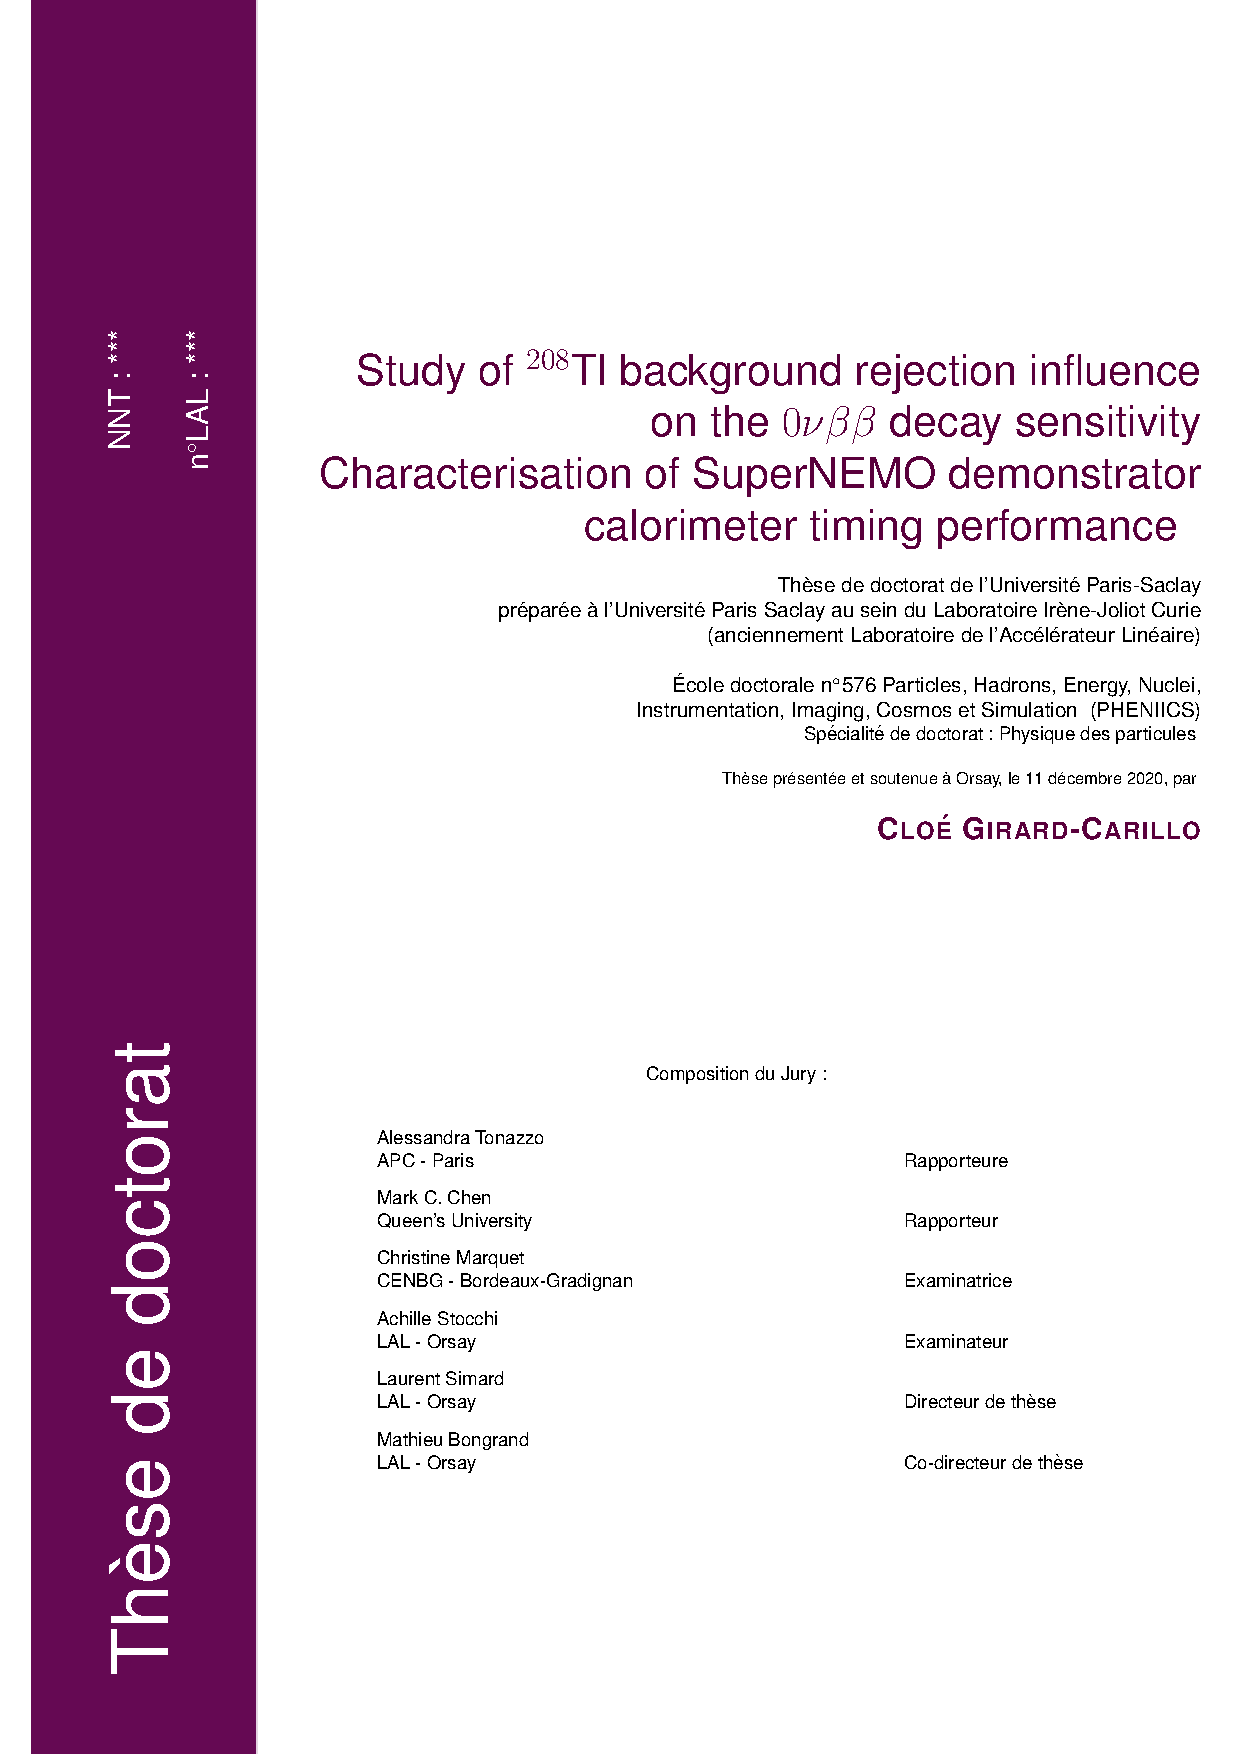
\includepdf{1couverture}
               \clearpage
               \chapter*{Acknowledgement}
\addcontentsline{toc}{chapter}{Acknowledgement}

Thanks.

               \cleardoublepage
               \tableofcontents


               \begingroup
               \setlength{\beforechapskip}{-35pt} % or any other dimension
               \chapter*{Introduction}
\label{ch:intro}
\addcontentsline{toc}{chapter}{Introduction}

It is always interesting to take a historical approach when talking about a scientific discovery. This allows us to put into perspective knowledge that is now considered to have been acquired.

The Standard Model of Elementary Particle Physics attempts to describe the world around us on scales that were inconceivable two centuries ago.
A little over a hundred years ago, Henri Becquerel discovered what we today call radioactivity, with the observation of $\beta$ decay.
This historical discovery was nevertheless accompanied by profound questioning, since the $\beta$ particle emitted during this decay, which turned out to be an electron, only carries away part of the available energy for the reaction.
This observation was contrary to the first principle of thermodynamics on the energy conservation, and some scientists postulated that this fundamental law was being violated.
It took 35 years for an eminent scientist by the name of Wolfgang Pauli to propose as a ``desperate remedy'' the existence of the \emph{neutrino} ($\nu$) - for small neutron in Italian - to explain the problem of missing energy.
Three years later Enrico Fermi laid the foundations for the first mathematical formulation of what is today the Lagrangian of weak interaction.
It was another 25 years, 60 years after the discovery of $\beta$ radioactivity, before the neutrino was experimentally observed by Clyde Cowan and Frederick Reines.
The neutrino adventure had only just begun.

Why is this particle, although abundantly produced in the sun in the atmosphere and in the earth, so difficult to detect?
It is because of its very low interacting rate with the matter - electrons and quarks - that constitutes us, being sensitive only to the weak interaction (of short range), and to the gravitational force (very weakly since the mass of the neutrino is extremely low, so much that it was believed massless for a long time).

In the current model of particle physics, neutrinos are actually described as massless.
It was Bruno Pontecorvo who proposed in 1957 that neutrinos could oscillate between their different mass states, based on the already known model of oscillation of neutral kaons.
To be valid, this model then presupposed that neutrinos had a non-zero mass.
It was the SuperKamiokande experiment that first observed this phenomenon in 1998, demonstrating that at least two of the three neutrino mass eigenstates have a non-zero mass.
The Standard Model of particle physics is then no longer sufficient to account for this particle properties, opening the way to physics beyond the Standard Model.

It now remains to be discovered how this particle acquires its mass.
Indeed, having a neutral charge under the three fundamental interactions described by the Standard Model, two mass generation mechanisms are foreseeable.
The first is to assume that, like all other fermions, the neutrino obtains its mass through the Higgs mechanism, leading irremediably to the assumption of the existence of a sterile neutrino.
The second, proposed by Ettore Majorana, assumes that the neutrino is its own antiparticle, giving the neutrino its mass with the addition in the Lagrangian of the Majorana mass term.
If this assertion is the one that applies to neutrinos, then a disintegration, prohibited in the Standard Model, is possible.
It is called \emph{neutrinoless double beta decay} ($\zeronu$), to contrast with the \emph{two neutrinos double beta decay} ($\twonu$) allowed by the Standard Model and already observed for several isotopes.
In the former disintegration, two simple $\beta$ decays take place simultaneously in the same nucleus, in which the two neutrinos are absorbed, allowing the total energy of the reaction to be distributed between the two exiting electrons.
For reasons that are detailed in the first chapter of this manuscript, which deals with the phenomenology of the neutrino, this disintegration is only possible if the neutrino is a Majorana particle.

Several experiments, also described in the first chapter, are dedicated to the search for this disintegration which, if it exists, is expected to be extremely rare.
%%Its observation would prove the neutrino is a Majorana particle.
The SuperNEMO experiment, on which I conducted my PhD, is one of them.
Successor of the NEMO experiments, it uses a unique combination of technologies, described in detail in the second chapter, allowing to trace the path of the electrons resulting from double $\beta$ disintegrations -with a wire chamber-, and also to measure their energies - with a segmented electromagnetic calorimeter.

These experiments differ from one another in the technology they use, and also in the sensitivity they can achieve in the search for this decay.
Within the framework of this PhD, I carried out a sensitivity study of this experiment presented in the third chapter, determining the influence that several characteristics of the detector can have on it.

All these experiments are designed to observe, should this process exist, an extremely rare physical event.
They are thus constrained to focus on the background which may disturb the measurement and have a non-negligible impact on their sensitivity to this disintegration.
In this perspective, the fourth chapter presents a new technique to identify the events resulting from one of the main background for this experiment, which is the natural disintegration of an isotope from the thorium 232 decay chain, found in the detector's sources.
To effectively reject this background, I am also studying the impact of the accuracy of the arrival time measurement in the calorimeter on sensitivity.
To complete this analysis based on detector simulations, the fifth chapter gives an overview of the data taken at Modane with the SuperNEMO calorimeter and of the analysis aiming to characterise the time resolution for a large part of the optical modules.

When I joined the LAL team at Orsay (now IJCLab) as a PhD student, SuperNEMO was already largely built in the Modane underground laboratory.
I had the opportunity to actively participate in the completion of its assembly, as well as in the analyses of the first commissioning data described in the last chapter, thus completing the experimental knowledge acquired during this PhD.

               \endgroup

               \chapter{Phenomenology of particle physics}
\section{The Standard Model of particle physics}
\subsection{Bosons}
\subsection{Fermions}
\subsection{$\twonu$ decay}
\subsection{Where the Standard Model ends}
\section{Going beyond the Standard Model with neutrinos}
\subsection{Neutrino flavors and oscillations}
\subsection{Neutrino masses and nature}
\label{subsec:nu_mass_nature}
\subsection{Other searches beyond the Standard Model with neutrinos}


               \begingroup
               \setlength{\beforechapskip}{-0.1pt} % or any other dimension
               \chapter{The SuperNemo demonstrator}
\label{ch:detector}

\section{The SuperNemo demonstrator}
\subsection{Comparison with Nemo$3$ experiment}
\subsection{Expermimental design}
\subsection{Sources}
\subsection{Tracker}
\subsection{Calorimeter}
\label{subsec:SN_calo}



\subsubsection{Scintillator}





\subsubsection{Photomultiplier}
\label{sec:calorimeter}
\subsection{Calibration systems}
\subsection{Control Monitoring system}
\subsection{Electronics}

\section{The backgroung of SuperNEMO}
\label{sec:SNbkg}
\subsection{Internal background}
\label{subsec:SNbkg_internal}

Trace quantities of naturally-occurring radioactive isotopes can occasionally produce two-electron events and thus can mimic $\beta\beta$-decay events.
The largest contributions come from isotopes of decay chains of $^{238}$U, $^{232}$Th and $^{40}$K, which disintegration occur inside the source foils, as well as inside the tracking volume.

Décire la contamination mesurée des sources, et du radon dans la partie suivante

\subsection{External background}
Radon:\\
Radon is a noble gas which occurs as an indirect decay product of uranium and thorium.
Due to its chemical properties, radon has a long diffusion length in solids, making it difficult to remove.
Radon contaminations inside the tracker volume is a major background to the rare event experiments such as SuperNEMO.
Simulations show that, to achieve the designed sensitivity, the level of radon must not exceed $0.15$ mBq/m$^{3}$ since its decay daughter \Bi, $\Qbb= 3.2$ MeV can mimic a $\zeronu$ event.
Radon concentration measurements inside the demonstrator tracker have been performed by the SuperNEMO collaboration, revealing an activity of $0.15\pm0.02$ mBq/m$^{3}$, through the combination of an anti-radon tent and an air-flushing method.

%%Repris d'un article -> a changer:
They are outgased in the air from the rock walls of the experimental hall and can enter the detector either through tiny gaps between sectors or through gas pipe joints.
The progeny of radon and thoron produces $\gamma$-rays and $\beta$ decays accompanied by internal conversion (IC), Møller or Compton scattering.
\subsection{Background specifications}
\subsection{Measured demonstrator background levels}

\section{Magnetic field}
\label{sec:magnetic_field}

It is, however, not high enough to impact significantly neither the few muons nor the $\alpha$ particles expected to be detected by the tracker.
Due to their much higher momenta, they will instead leave straight tracks in the wire chamber.

\section{The SuperNemo software}
\label{sec:SNsoftware}
\subsection{Simulation}

As described in Sec.~\ref{sec:SNsoftware} of Chapter~\ref{ch:detector}, the SuperNEMO collaboration developed its own simulation, reconstruction and analysis environment.
The Falaise software, specifically designed by and for the SuperNEMO collaboration, holds the \verb!C++! library for the event reconstruction and analysis of simulated and real data.
Especially, it contains the geometry, the detector material, the event data model, the reconstruction algorithms and the data analysis.
Finally, the SNFee software is a tool package for the configuration, control and monitoring of the SuperNEMO front-end electronics.

\subsection{Reconstruction}

               \endgroup

               \chapter{Sensitivity of the SuperNEMO demonstrator to the $\zeronu$}
\label{ch:sensitivity}

A study aiming to evaluate the SuperNEMO sensitivity to the $\zeronu$ decay, and the corresponding effective neutrino mass is presented.
From previous studies, the final detector is expected to exclude half-lives up to $1\times 10^{26}$~y ($90\%$ CL), with an exposure of $500$~kg.y with \Se\ sources\footnote{Supposing the $\zeronu$ decay of \Se\ occurs through the exchange of a light Majorana neutrino.}~\cite{art:SuperNEMO2010}.
The SuperNEMO demonstrator was designed in order to assess the technical feasibility of such a large-scale detector and to show that background specifications can be achieved.
With a reduced exposure of $17.5$~kg.y, this demonstrator is expected to reach a sensitivity on the $\zeronu$ process of $5.3\times~10^{24}$~y ($90\%$ CL)~\cite{CalvezThesis}.

As it was the case with its predecessor, a copper coil was designed to deliver a magnetic field inside the wire chamber, to bend the charged particles trajectories, hence making it possible to discriminate between electrons and positrons.
However, studies led by the collaboration determined that the intensity of this field could be modified by the photomultiplier magnetic shields.
Photomultipliers energy resolution could also be impacted by the presence of this magnetic field~\cite{CalvezThesis,internal:magnetic_field}.
We aim to explore the impact, on both the demonstrator and final detector sensitivity, of the presence of this magnetic field.
The findings of this study participate in better understanding the detector performances.
In a context of investigating the demonstrator and final detector's capabilities, different internal source contamination levels are considered to estimate the sensitivity.
The topology of interest is that of two electrons, and we use the total energy sum to discriminate the signal from the background events.
Thanks to SuperNEMO tracking capabilities, extra topological informations are exploited to improve the final sensitivity.
To go further, we also explore the possibility of studying the $\zeronu$ decay of other $\beta\beta$ isotopes.

\section{The $\zeronu$ signal and background model}
\label{sec:sensitivity_simus}

A full GEANT$4$ simulation of the demonstrator was performed to determine the lower limit on the $\zeronu$ half-life that can be probed with SuperNEMO in case of the non-observation of the signal.
Due to the time it would take to simulate every background contribution, we choose a simplified model where only the most harmful backgrounds to the $\zeronu$ decay search are simulated.
In addition, $\zeronu$ signal decays inside the detector are simulated, to better understand all the aspects of this analysis.

\subsection{The $\zeronu$ signal}

The SuperNEMO detector was designed to search for the yet never-observed $\zeronu$ decay.
In the following, we assume the underlying mechanism for this decay is the exchange of a light Majorana neutrino, the so-called mass mechanism (MM), as it is the most widespread.
The hypothetical $\zeronu$ signal would be detected as an excess of events at the end point of the $\twonu$ spectrum, with respect to the predicted background contamination levels.

\subsection{Inside detector backgrounds}

Numerous types of backgrounds that could mimic and hinder the search for the $\zeronu$ signal were simulated.

\subsubsection{Internal backgrounds}

As explained is Chapter~\ref{ch:detector}, internal backgrounds stand for decays occurring inside the source foils, presenting the same signature as the $\zeronu$ signal.
These backgrounds are mainly the $\twonu$ decay undergone by the source isotope, disintegrations of \Tl\ and \Bi\ contaminations inside the source foils, as well as \Bi\ disintegrations due to Radon deposited on the surface of the source foils.

\subsubsection*{The $\twonu$ process}

In the full energy range, the allowed $\twonu$ decay of \Se\ stands as the dominant internal background type.
The corresponding two-electrons energy sum spectrum is a continuum, whose ending point should stands at $\Qbb = 2.99$~MeV, but is subtly shifted by the detector's energy resolution due to energy losses inside the source foils and gaseous detector.
A total of $10^{7}$ events of this decay were simulated inside the source foils, in the full energy window.
However, above a certain energy value, the number of $\twonu$ events decreases strongly, which can lead to a lack of statistics in a energy region favourable for the search for $\zeronu$ signal.
To offset this effect, additional $10^{7}$ of this decay were simulated on a slightly reduced energy range, that is to say above $2$~MeV.
The second set of simulations is normalised with the first one.
In this way, the lack of $\twonu$ simulated events in the high-energy tail is avoided, without requiring too high computational resources.

\subsubsection*{Source foils contamination by natural isotopes}

As described in Sec.~\ref{subsec:SNbkg_internal}, after sources purification, residual natural isotopes such as \Tl\ or \Bi\ can still be present inside the foils, constituting the principal internal source of background, with the $\twonu$ decay.

\subsubsection{Tracker contamination by natural isotopes}

Radon, a descendant of \U, is present as a gas in the tracker.
Its daughter isotopes, when deposited on the tracker wires, can produce events similar to internal ones.
In fact, one of the progeny of \Rn, the \Bi, can decay on (or near) a foil, and appear with a two-electron topology, becoming hard to distinguish from a double beta decay candidate.
As this isotope is distributed throughout the whole tracking detection volume, a large quantity of this decay were simulated on the tracker wires.
%This way, we maximise the amount of \Bi\ events, coming from \Rn\ decays, in the region of interest.


\subsection{External backgrounds}
\label{subsec:ext_bkg}

This background category was described in detail in Sec.~\ref{subsec:SNexternal_bkg}.
As a reminder, it is populated by the external $\gamma$-ray flux produced by radioactive isotope decays (mostly \K, \Bi\ and \Tl) in detector components or surrounding laboratory rocks, as well as neutron interactions in the external iron shield.
As simulating external backgrounds would be very consuming in terms of computing resources due to their very low probability to produce two electrons ($2e$) topologies, they were not simulated in the framework of this analysis.
Nevertheless, a future study would consider their contribution, especially to evaluate the impact of the magnetic field on the sensitivity.

\subsection{Expected number of decays}

The number of natural isotope decay events expected in the $2e$ topology depends on their activities inside the source foils (for \Tl\ and \Bi), or on the tracker's wires (for \Rn\ decaying in \Bi).
The amount of expected double $\beta$ decays is driven by its half-life value: the higher the half-life, the lower its contribution in the total number of expected background.
For this analysis, we consider the $\twonu$ half-life of \Se\ measured by NEMO-$3$, $\Ttwonu~=~9.39~\pm~0.17$~(stat)~$\pm~0.58$~(syst)~$\times~10^{19}$~years~\cite{art:NEMO2018}.
For the $\zeronu$ process, we also take the best limit set by the NEMO-$3$ detector, $\Tbeta > 2.5\times 10^{23}$~y~\cite{art:NEMO2018}.
This value is given for illustration purposes only, as it is not used to estimate the sensitivity of the detector.

Tab.~\ref{tab:sensitivity_simulations} gives the expected number of background events, for the demonstrator and final detector exposures, assuming target background activities are reached: $\mathcal{A}^{\text{Tl}}=10~\mu$Bq/kg, $\mathcal{A}^{\text{Bi}}=2~\mu$Bq/kg and $\mathcal{A}^{\text{Rn}}=0.15$~mBq/m$^{3}$.
The expected number of disintegrations do not take into account any technique to reject background, and are given for the full energy range of the two measured electrons.
\begin{table}[h!]
  \centering
  \begin{tabular}{|c|l|cc|}
    \hline
    Process & Half-life/Activity &\multicolumn{2}{c|}{Expected decays} \\
    && Demonstrator & Final detector \\
    \hline\hline
    $\twonu$ & $\Ttwonu = 9.39\times 10^{19}$ y & $9.5\times 10^{5}$ & $2.7\times 10^{7}$  \\
    \Tl\ & $\mathcal{A}^{\text{Tl}} = 2~\mu$Bq/kg  & $1.1\times 10^{3}$ & $3.1\times 10^{4}$  \\
    \Bi\ & $\mathcal{A}^{\text{Bi}} = 10~\mu$Bq/kg & $5.5\times 10^{3}$ & $1.6\times 10^{5}$ \\
    \Rn\ & $\mathcal{A}^{\text{Rn}} = 0.15$ mBq/m$^{3}$ & $1.8\times 10^{5}$ & $7.2\times 10^{6}$ \\
    \hline
  \end{tabular}
  \caption{Expected number of background events, for the demonstrator ($17.5$ kg.y) and for the final detector ($500$ kg.y).
    We assume target background activities are reached: $\mathcal{A}^{\text{Tl}}~=~10\,\mu$Bq/kg, $\mathcal{A}^{\text{Bi}}~=~2\,\mu$Bq/kg, $\mathcal{A}^{\text{Rn}}~=~0.15$ mBq/m$^{3}$.
    The measured half-life $\Ttwonu~=~9.39\times~10^{19}$ y for \Se\ is considered~\cite{art:NEMO2018}.
    \label{tab:sensitivity_simulations}}
\end{table}

However, they are expected to be extremely reduced, notably by the application of event selections aimed at maximising the sensitivity to the $\zeronu$ half-life.
Especially, in the following, we focus on an optimised narrow energy window, called \emph{region of interest}, whose usefulness is described in detail in the next section.
This is also one of the reasons why it was necessary to simulate a large number of events, so that the signal and backgrounds are correctly represented in the region of interest.


\section{Event selection}
\label{sec:sensitivity_ev_selection}

For SuperNEMO, the $\zeronu$ signature is two-electrons events, emitted simultaneously from the same vertex on the source foils, with an energy sum compatible with $\Qbb = 2.99$~MeV for \Se\ sources.
Therefore, we conducted this analysis selecting only events matching the $2e$ topology.

\subsection{Electron definition}

A reconstructed particle is tagged as an electron if it has:
\begin{itemize}
\item a vertex on the source foil,
\item a reconstructed track inside the wire chamber,
\item an associated calorimeter hit,
\item and a final criterion applied only if the magnetic field is simulated inside the tracker.
\end{itemize}
About the last point, as announced, we aim at studying the influence of the magnetic field on the final sensitivity results.
To this end, we are led to consider two separate cases, one where the magnetic field is switched on, aligned with the $Z$ (vertical) axis of the detector, with a uniform value of $25$ Gauss, and one where it is switched off.
In the first case, particles such as electrons and positrons of a few~MeV have a curved trajectory in the tracker.
In the second case, the tracks of the particles may be similar to straight lines (not to mention the possible multiple scattering on the tracker wires).
It is then necessary to adapt the selection of events to each case.
When the magnetic field is on, we consider a fourth criterion: a particle is identified as an electron if its track has a negative curvature\footnote{A trajectory is said by convention to be negative if it has the same curvature as that of an electron moving from the source to the calorimeter, in a magnetic field oriented according to $+Z$.}.
In the following, we present results where the magnetic field is turned on.
The off-field study is addressed in Sec.~\ref{subsec:field}.

A two-electron ($2e$) topology is then defined as two reconstructed tracks with negative curvatures, each one associated with a vertex on the source foils and a calorimeter hit.
These selections represent the so-called \emph{first-order} cut-offs.
The $2e$ topologies have been selected using the Particle Identification module at the end of the Falaise reconstruction pipeline~\cite{CalvezThesis}.
I wrote my own module and added it to the collaboration software in order to store the selected events in a data format matching my off-line analysis chain.
Second order selections taking into account topological information (time of flight, location of vertices on the source foils) are presented in Sec.~\ref{sec:demonstrator_sensitivity}.

\subsection{Total energy spectrum}

In Fig.~\ref{fig:energy_spectra}, we present the total energy spectra for each simulated process in the $2e$ topology, after application of the first-order cut-offs.
The distributions are given for the demonstrator (\Se\ sources, $17.5$~kg.y exposure), considering the specified activities are reached.
Once again, the $\zeronu$ spectrum is given only for illustrative purposes.
If this decay is detected, its two-electrons energy sum distribution would be a peak, located at the end-point of the $\twonu$ energy distribution, that is to say at the total available energy, $\Qbb = 2.99$~MeV.
As the two electrons of this decay would share the total available energy, this peak should be infinitely thin.
However, a widening of this distribution is expected, mainly due to the calorimeter energy resolution as well as energy losses inside the dense source material.
Indeed, the path of an electron in the source is more or less long, depending on the disintegration location and on the emission angle, leading to a degradation of the measured energy.
\begin{figure}[h!]
\centering
\begin{subfigure}[t]{0.9\textwidth}
  \centering
  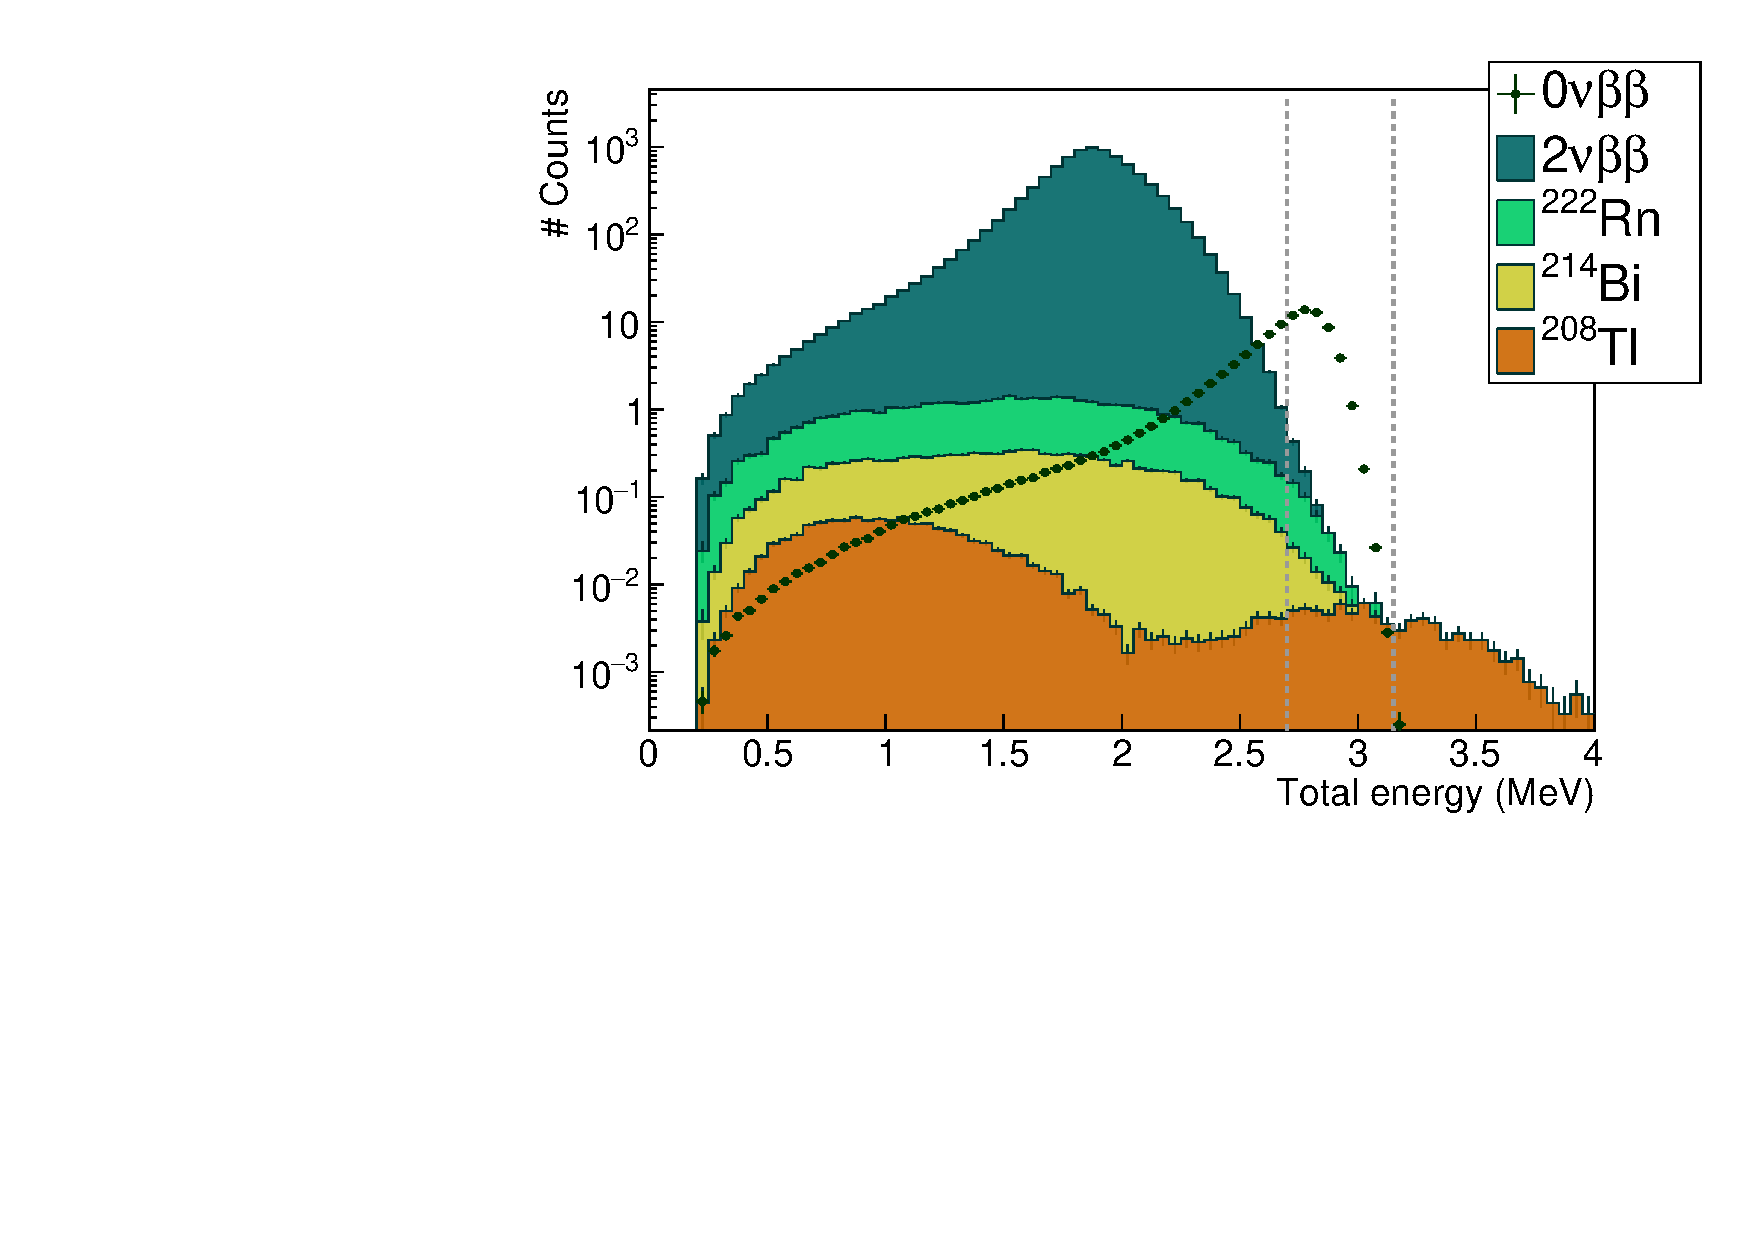
\includegraphics[width=0.95\textwidth]{Sensitivity/fig_sensitivity/energy_spectrum_with_B_82Se.pdf}
  \captionsetup{justification=centering}
  \caption{Full energy range.
    \label{subfig:energy_spectra_full}}
\end{subfigure}
\vskip\baselineskip
\vskip\baselineskip
\begin{subfigure}[t]{0.9\textwidth}
  \centering
  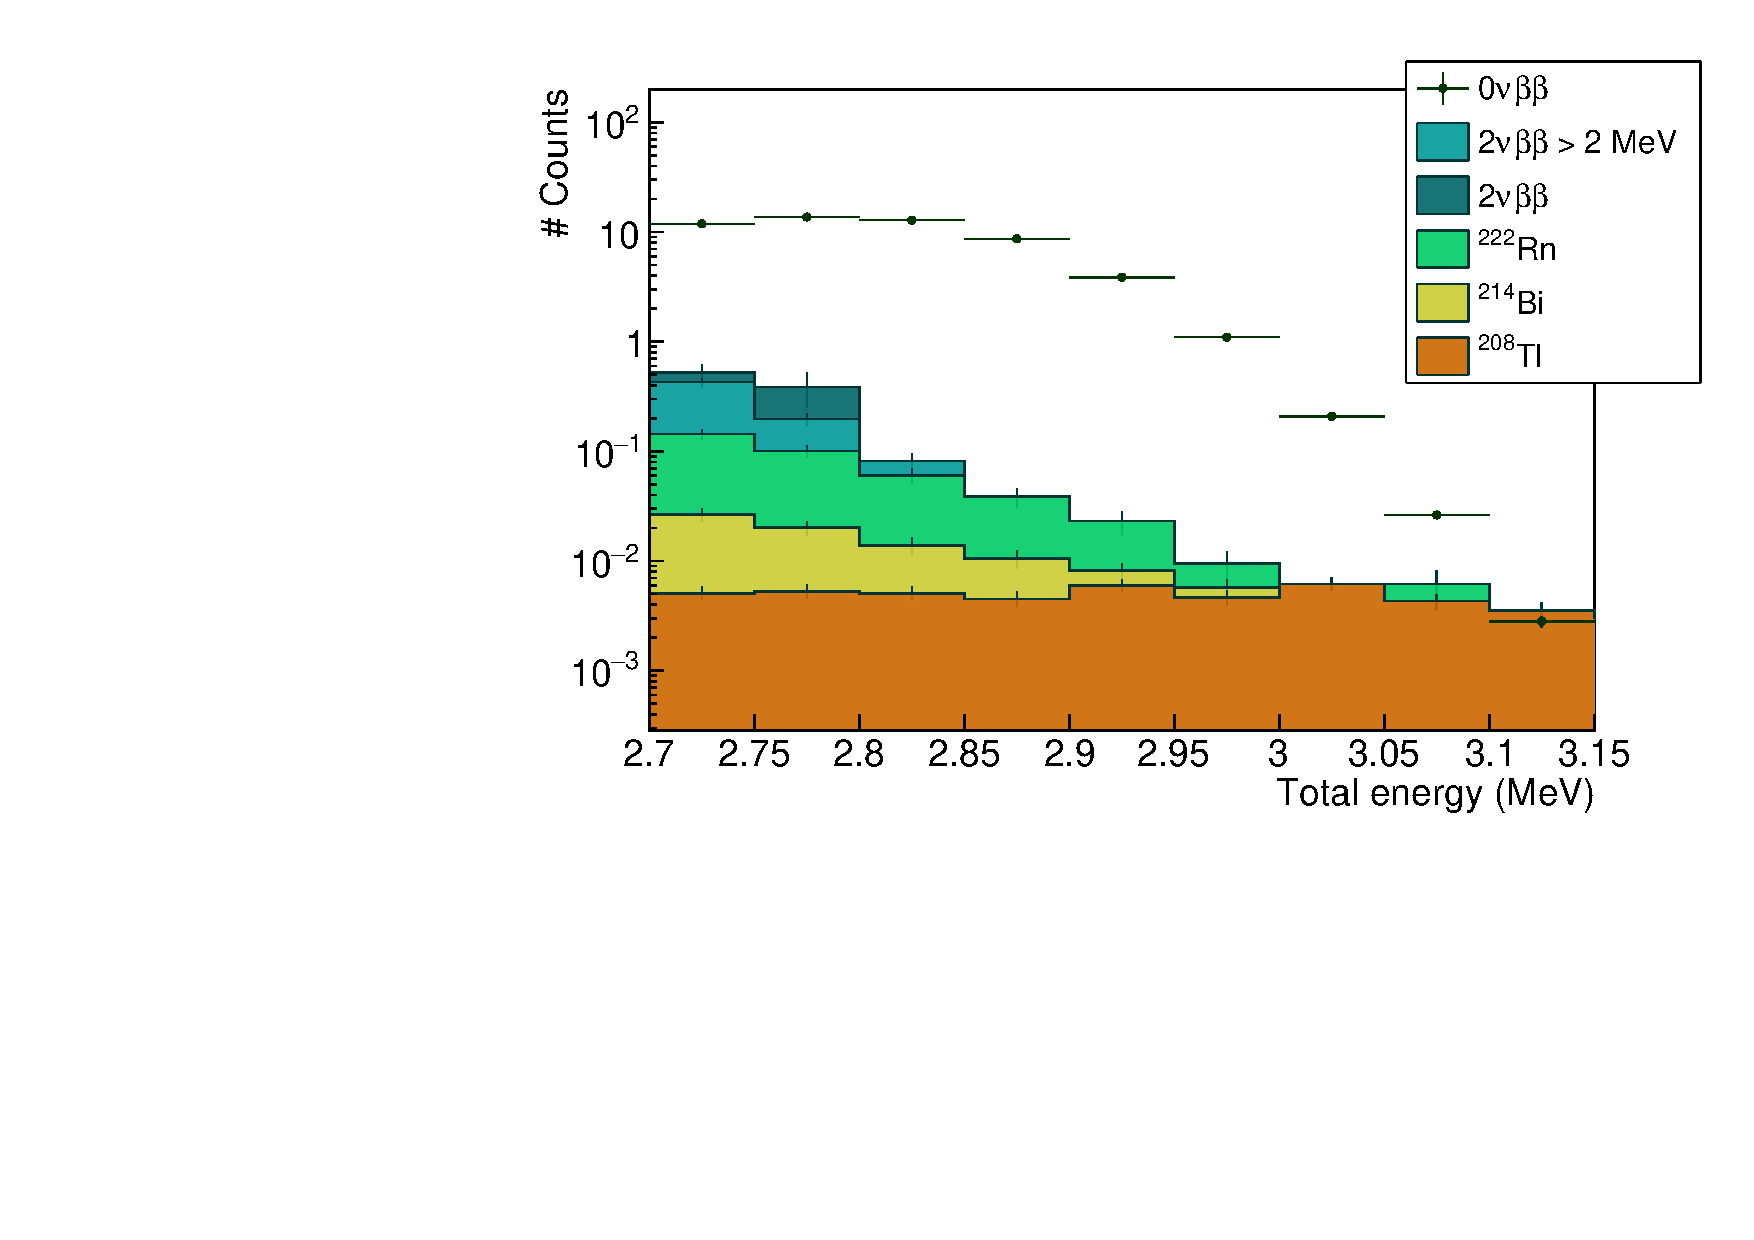
\includegraphics[width=0.95\textwidth]{Sensitivity/fig_sensitivity/energy_spectrum_with_B_82Se_zoom.pdf}
  \captionsetup{justification=centering}
  \caption{Zoom on ROI.
    \label{subfig:energy_spectra_zoom}}
\end{subfigure}
\caption{Total energy spectra for the $\zeronu$ signal and main backgrounds, for (a) the full energy range, and (b) for the [$2.7$;$3.15$]~MeV energy range, whose optimisation is discussed in Sec.~\ref{sec:Nbkg_ROI}.
  The $\twonu$ spectrum is normalised to $\Ttwonu~=~9.39\times~10^{19}$~y, and the specified activities are considered for \Tl,\Bi\ and \Rn.
  The amplitude of the $\zeronu$ is arbitrarily set at the limit obtained with NEMO-$3$.
  \label{fig:energy_spectra}}
\end{figure}

As explained in Sec.~\ref{sec:sensitivity_simus}, two sets of $\twonu$ events were simulated: one on the full energy range, and one for which the two-electrons energy sum is greater than $2$~MeV.
After the normalisation of these two sets, we get the complete $\twonu$ energy spectrum displayed in the figure.
These energy spectra confirm the $\twonu$ background is dominant in the total energy range.

The \Tl\ total energy spectrum extends up to high energies.
  It reveals two distinct peaks, one corresponding to a low-energy $\beta$ particle, the other to the internal conversion of the $2.614$~MeV gamma, emitted after \Tl\ $\beta^{-}$ disintegrations (Sec.~\ref{subsec:SNbkg_internal}).
Whatever their origin, either \Rn\ contaminations inside the tracker gas, or internal contaminations of the source foils, the two \Bi\ energy distributions have nearly the same shapes.

% The progeny of \Rn\ produces $\gamma$-rays and $\beta$ decays accompanied by internal conversion (IC), Møller or Compton scattering, the dominant mechanism being the first one.
%%Therefore, given the activities of \Rn\ in the tracker and \Bi\ inside the source foils, theses two background types both contribute at the same level in the full energy range.
A widespread technique consists in constraining the $\zeronu$ decay searches to a narrow energy range, the so-called \emph{region of interest} (ROI).
It allows to reduce the expected number background decays, while improving the chances to observe the signal decay, then maximising the limit set on $\Tbeta$.
A typical ROI is materialised in the figure by two vertical dashed lines, revealing \Tl, \Bi\ and \Rn\ could be harmful for the search for the $\zeronu$ decay.
The influence of the sources contamination by these natural isotopes, as well as optimised background rejection techniques are presented in Sec.~\ref{sec:demonstrator_sensitivity}.

In the following, we expose general principles leading to the determination of the best limit on $\Tbeta$, in the appropriate region of interest.
We illustrate the reasoning by applying it on the demonstrator case, with specified activities, and on-magnetic field condition.
However, the technique presented remain valid for all exposures, internal contamination levels and field conditions.


\section{Demonstrator sensitivity to the $\zeronu$ decay of \Se}
\label{sec:Nbkg_ROI}

The SuperNEMO demonstrator is designed to measure $\beta\beta$ decays of radioactive emitters.
In case a the non-observation of the $\zeronu$ process, the collaboration would set a lower-limit on the half-life $\Tbeta$, and an upper-limit on the effective neutrino mass $\mbb$.

\subsection{Sensitivity to the $\zeronu$ half-life}

In case of the non-observation of a $\zeronu$ signal, the expected lower limit on the half-life is provided for a given energy range [$E_{\text{min}}$;$E_{\text{max}}$] on the two electrons energy sum, and depends on the characteristics of the detector.
Firstly, it depends on the signal detection efficiency, $\epsilon_{0\nu}$ in this energy window, which corresponds to the ratio of the number of selected signal events to the number of simulated ones.
It also depends on the source isotope nature, as well as on the detector exposure $m\times t$, with $m$ the mass of source material in the foils and $t$ the data acquisition time period.
It follows
\begin{equation}
  \Tbeta > \frac{\mathcal{N}_{\text{A}}\ln{2}}{M}\times \frac{\epsilon_{0\nu}\times m\times t}{N_{0\nu}^{\text{excl.}}}\,,
  \label{eq:tbeta_limit}
\end{equation}
with $\mathcal{N}_{\text{A}}$ the Avogadro number and $M$ the $\beta\beta$ emitter molar mass.
$N_{0\nu}^{\text{excl.}}$ is the number of signal events excluded at a given confidence level (usually $90$\%), calculated with the Feldman-Cousins statistics from the total expected number of background events.
The Feldman-Cousins statistics~\cite{art:feld-cous} is a wide-used method in rare events search experiments, providing confidence intervals for upper limits in the case of background events following a Poissonian probability law.
We use this method in the framework of this analysis to provide a limit, at $90\%$ CL, on the number of excluded signal events $N_{0\nu}^{\text{excl.}}$, on the basis of the expected number of background events, given below.
\begin{itemize}
\item The $\twonu$ background\\
  Eq.~\eqref{eq:tbeta_limit} defines the lower limit on $\Tbeta$ from the number of excluded signal events, and the signal selection efficiency $\epsilon_{0\nu}$.
  In a similar manner, we can define the number of expected $\twonu$ events, $N_{2\nu}$, from the half-life $\Ttwonu$ and the $\twonu$ selection efficiency, $\epsilon_{2\nu}$, as
  \begin{equation}
    N_{2\nu} = \frac{\mathcal{N}_{\text{A}}\ln{2}}{M}\times\frac{\epsilon_{2\nu}\times m\times t}{\Ttwonu}\,.
    \label{eq:N_2nu}
  \end{equation}
\item Natural radioactive backgrounds\\
  We consider the background selection efficiencies $\epsilon_{\text{rad.}}$ in a given energy window.
  The number of background events is therefore given, for the \Tl\ and \Bi\ internal contaminations, as
  \begin{equation}
    N_{\text{rad.}}^{m} = A_{\text{rad.}}^{m}\epsilon_{\text{rad.}}\times m\times t\,,
  \end{equation}
  where $A_{\text{rad.}}^{m}$ is the activity given in Bq/kg.
  Similarly, for the \Rn\ background,
  \begin{equation}
    N_{\text{rad.}}^{V} = A_{\text{rad.}}^{V}\epsilon_{\text{rad.}}\times V\times t\,,
    \label{eq:N_Rn}
  \end{equation}
  with $V = 15.3$ m$^{3}$ the total tracker volume, and $A_{\text{rad.}}^{V}$ represents here a volumic activity, given in Bq/m$^{3}$.
\end{itemize}

As we said, all equations from Eq.~\eqref{eq:tbeta_limit}~to~\eqref{eq:N_Rn} are valid for a given energy range [$E_{\text{min}}$;$E_{\text{max}}$].
To find the optimal energy interval for the search for the $\zeronu$ decay, that is to say the one maximising the limit on $\Tbeta$, we must study the influence of the variations of E$_{\text{min}}$ and E$_{\text{max}}$ bounds on the final sensitivity.
On Fig.~\ref{fig:energy_spectra}, we observe that beyond the energy sum of $3$~MeV, the total number of background events is highly reduced, and the \Tl\ background dominates, with $0.03$ count expected for E$>3.2$~MeV.
This is why the upper limit E$_{\text{max}}$ of the energy interval has only a limited impact on the search for the best ROI.
It is then natural to study mainly the influence of the lower limit E$_{\text{min}}$.
%% In that purpose, the selection efficiencies, entering in the calculation of the $\Tbeta$ lower
%% limit, are presented in Fig.~\ref{fig:efficiency_spectra}, as a function of the lower bound
%% $\text{E}_{\text{min}}$.

In Fig.~\ref{fig:sensitivity_cont} is presented the variations of sensitivity with the ROI upper and lower bounds.
We found that, for the demonstrator exposure, with \Se\ sources and a $25$ Gauss magnetic field, and for the specified background activities, the best ROI is [$2.7$;$3.15$]~MeV.
As expected, as long as the upper bound is larger than $3.15$~MeV, the sensitivity on the search for $\zeronu$ is not affected.
Therefore, this value is kept in order to enter into a future more general study, taking into account the neutron background of the experiment, which extends at high energies.
In the optimised [$2.7$;$3.15$]~MeV energy range, the sensitivity expected for the SuperNEMO demonstrator stands at
\begin{equation}
\Tbeta > 5.7\times 10^{24}\,\text{y}\qquad (90\% \text{CL})\,.
\end{equation}
This result is compatible with the previous SuperNEMO analysis led by Steven Calvez~\cite{CalvezThesis}.
\begin{figure}[h!]
  \centering
  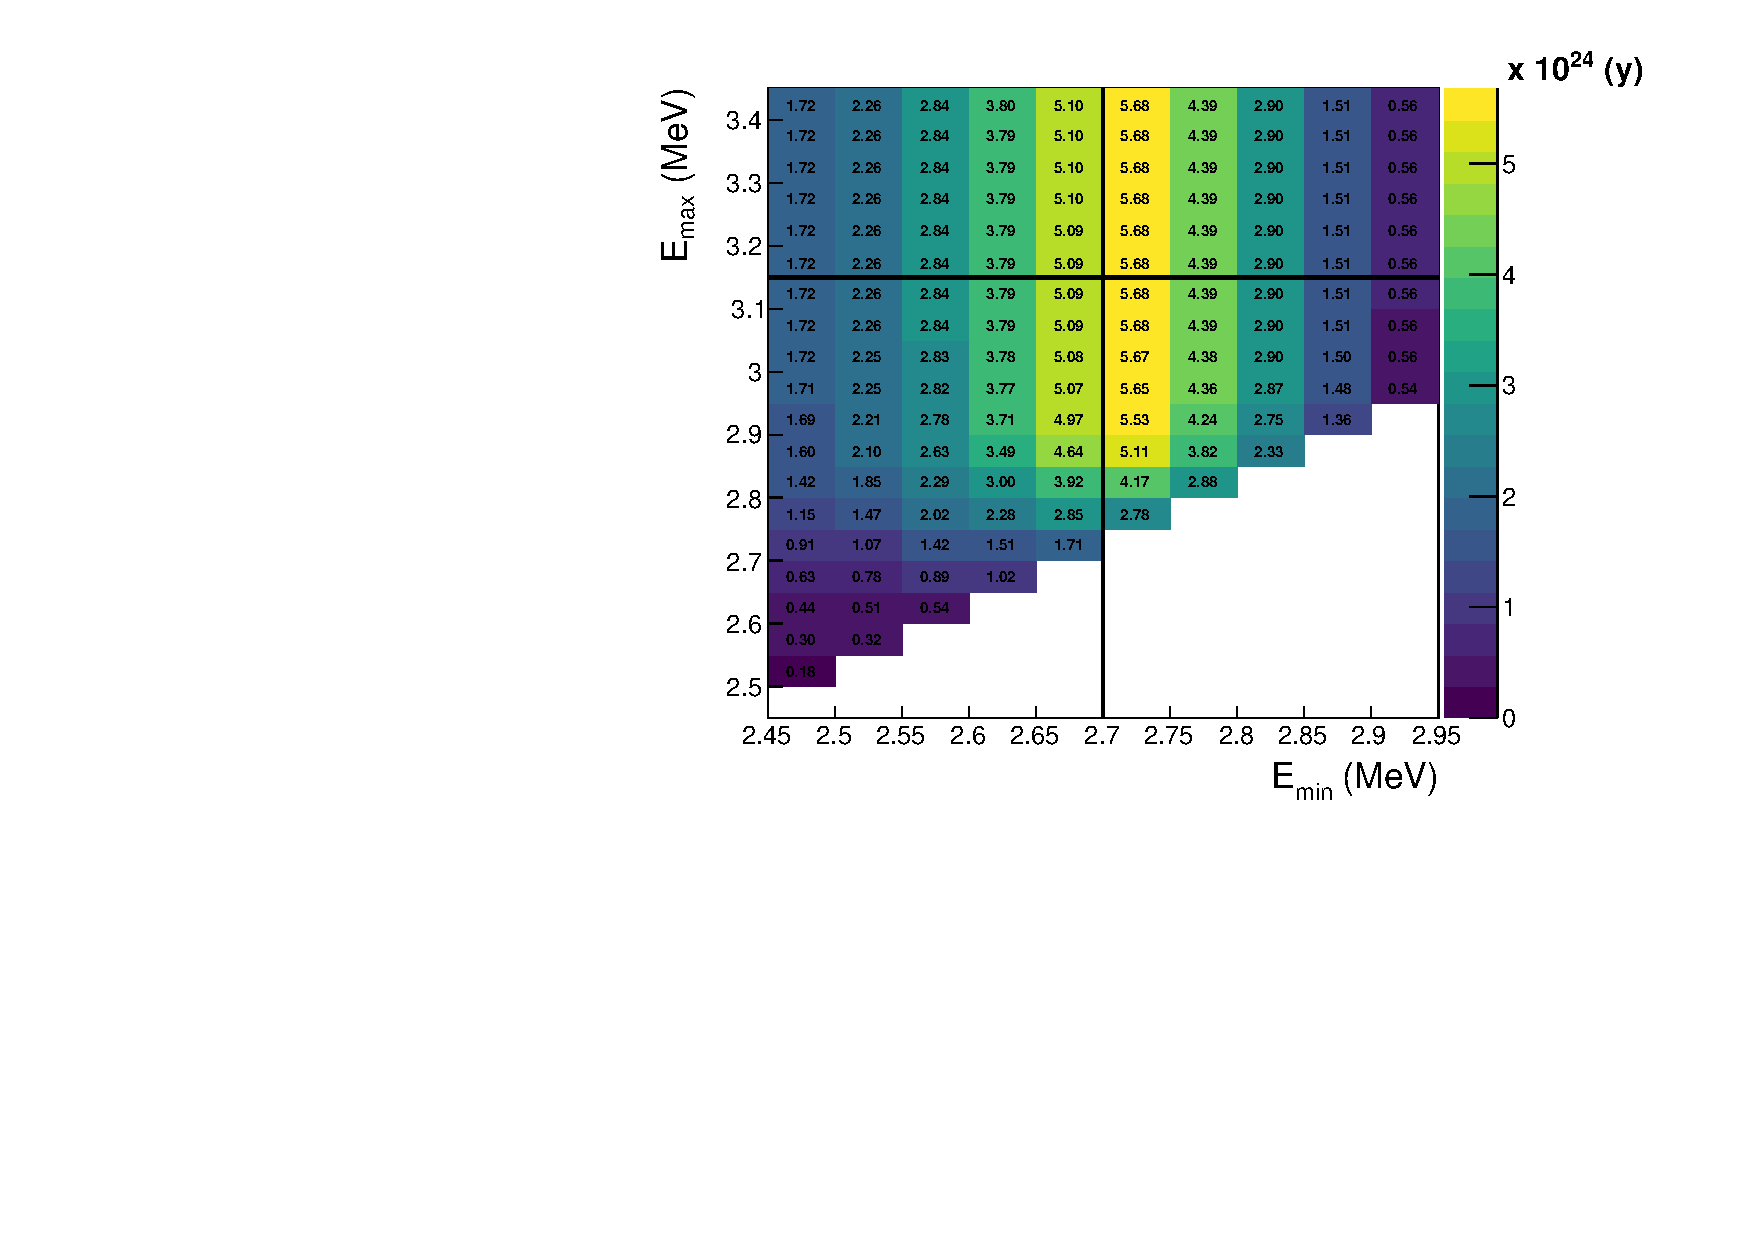
\includegraphics[width=1.1\textwidth]{Sensitivity/fig_sensitivity/sensitivity_spectrum_with_B_82Se.pdf}
  \caption{Two-dimensional histogram showing the evolution of the $\Tbeta$ $90$\% limit as a function of the ROI lower and upper energy bounds.
    The maximal lower limit of $\Tbeta~>~5.7\times~10^{24}$~y (90\%~CL) is retained, in the [$2.7$;$3.15$]~MeV region of interest.
    \label{fig:sensitivity_cont}}
\end{figure}

Tab.~\ref{tab:eff_nominal_ROI} summarises the expected number of background events.
%% \begin{figure}[h!]
%%   \centering
%%   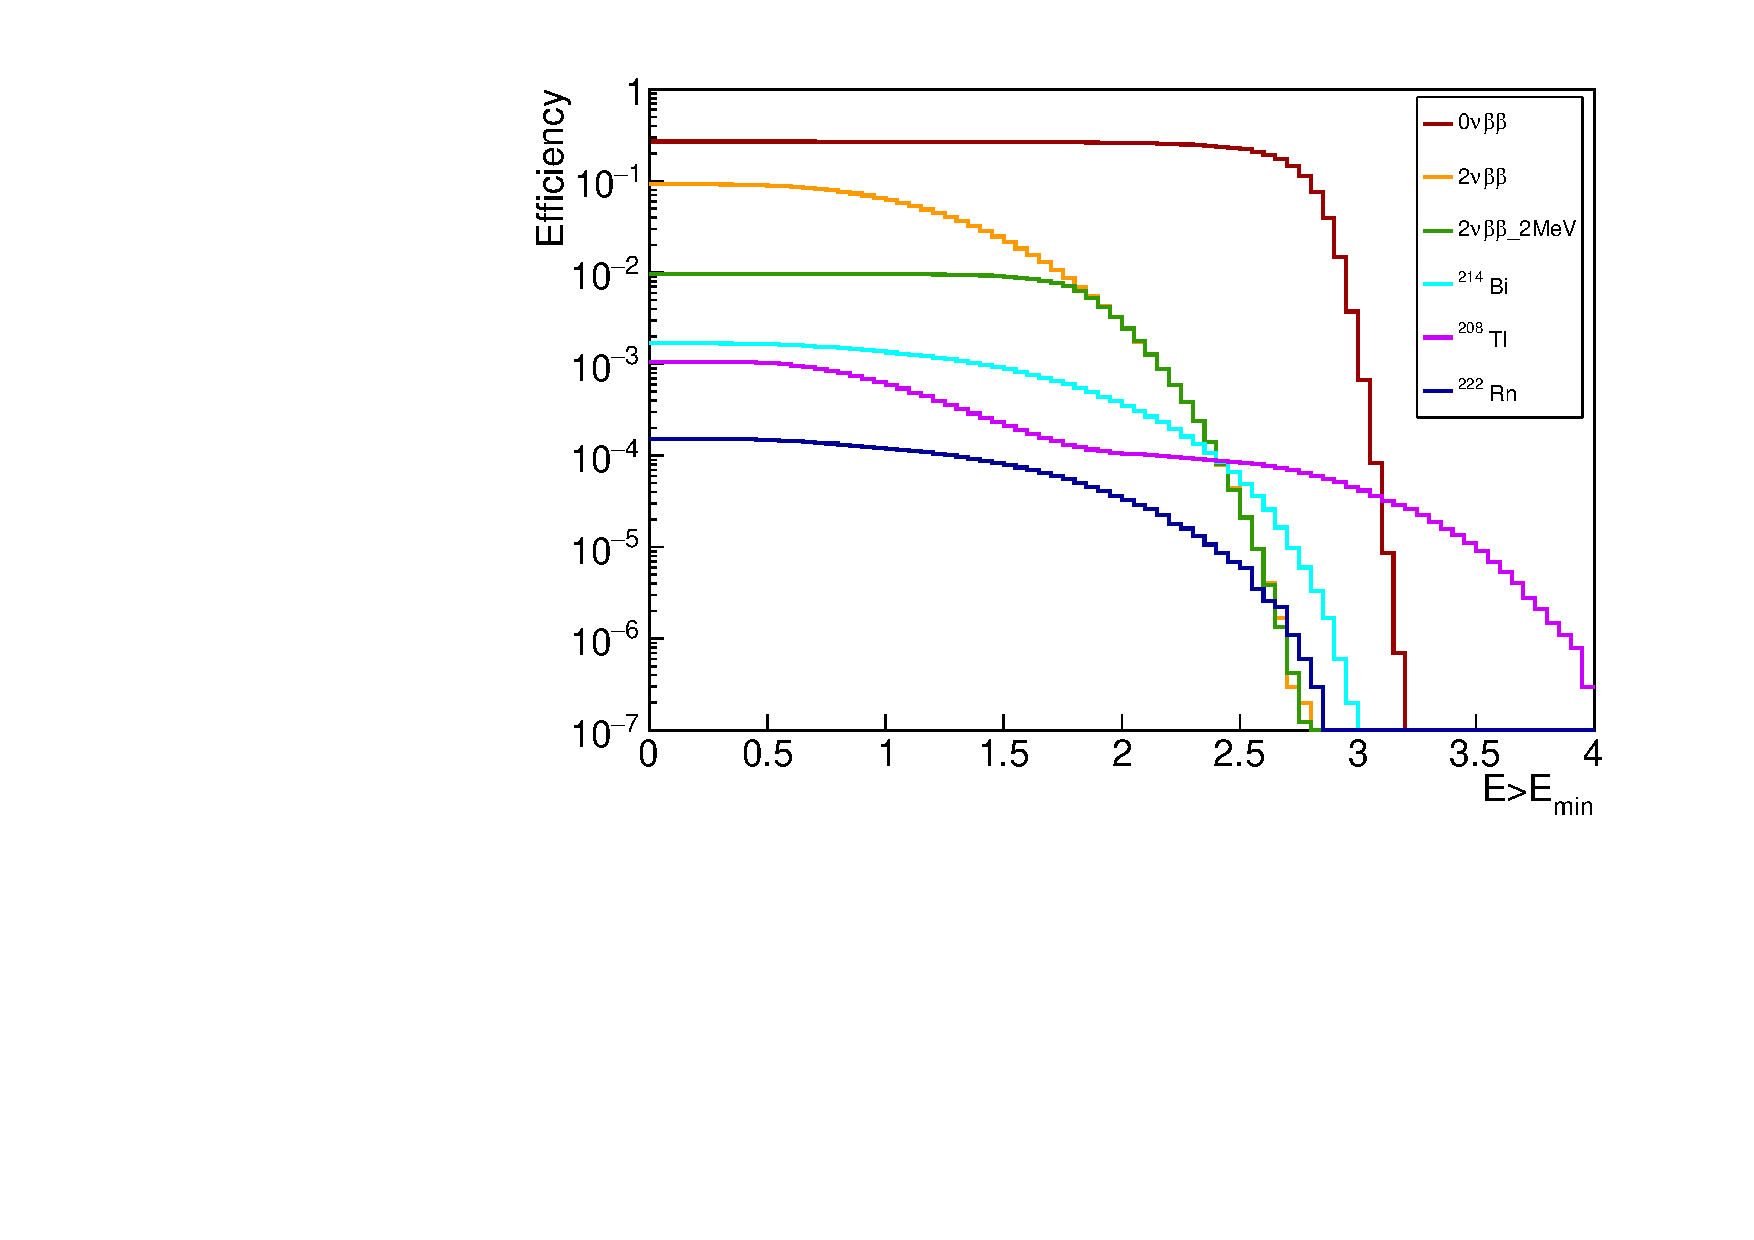
\includegraphics[width=0.8\textwidth]{Sensitivity/fig_sensitivity/efficiency_spectrum_with_B_82Se.pdf}
%%   \caption{Efficiency spectra as a function of $\text{E}>\text{E}_{\text{min}}$, for the $\zeronu$ signal (dashed black line) and for the main backgrounds (plain lines).
%%     The two vertical grey lines depict the final ROI optimised for the case of the demonstrator, taken the specified isotope activities.
%%     \label{fig:efficiency_spectra}}
%% \end{figure}
As a matter of fact, the ROI would correspond to an energy range where background selection efficiencies are low, in order to maximise the $\Tbeta$.
The dominating background in this range remains the $\twonu$ decay.
\begin{table}[h!]
  \centering
  \begin{tabular}{|c|c|}
    \hline
    Process & Event selection \\
    \hline\hline
    $\epsilon_{0\nu}$ & $14.7$\% \\
    \hdashline
    $\twonu$  & $0.418$ \\
    \Tl  & $0.0475$  \\
    \Bi  & $0.0546$   \\
    \Rn  & $0.292$  \\
    Total & $0.394$ \\
    \hline
  \end{tabular}
  \caption{Selection efficiency of $\zeronu$ events and expected number of backgrounds events in the optimised ROI [$2.7$;$3.15$]~MeV, for the exposure of the SuperNEMO demonstrator (17.5 kg.y).
    The specified levels of contamination are considered.
    \label{tab:eff_nominal_ROI}}
\end{table}



\subsection{Limit on the effective neutrino mass}

The decay rate for the light Majorana exchange mechanism is given by:
\begin{equation}
  (T_{1/2}^{0\nu})^{-1} = g_{A}^{4}G^{0\nu}|M^{0\nu}|^{2}\left\lvert\dfrac{m_{\beta\beta}}{m_{e}}\right\rvert^{2}\,.
\end{equation}
where $G^{0\nu}$ is the two particles phase space factors, depending on $\Qbb$ and Z the number of protons, $M^{0\nu}$ is the nuclear matrix elements for the $\zeronu$ process, and $\mbb$ is the effective Majorana neutrino mass, defined as
\begin{equation}
  \langle \mbb \rangle = \left\vert \Sigma_{i}m_{i}U^{2}_{ei} \right\vert \,,
\end{equation}
where $m_{i}$ are the neutrino masses, and $U^{2}_{ei}$ is the mixing matrix.
Therefore, the effective mass takes into account the neutrino mixing.
Consequently, observing the $\zeronu$ decay would not only prove the Majorana nature of neutrinos but, assuming the mass mechanism, could also help constraining the absolute neutrino masses.
Given $g_{A}$, $G^{0\nu}$ and $M^{0\nu}$~\cite{PhysRevC.85.034316,PhysRevC.83.034320}, we find the SuperNEMO demonstrator could reach a limit on the effective neutrino mass of
\begin{equation}
\langle\mbb\rangle < [0.24-0.47]~\text{eV}\qquad (90\% \text{CL})\,.
\end{equation}
Although this limit is not competitive with other current $\zeronu$ experiments, this is an improvement compared to NEMO-$3$, demonstrating that SuperNEMO's technology would benefit from being adapted to larger scales.

In this section, we presented the general procedure leading to an optimised result on the $\Tbeta$ limit, and provided it for the SuperNEMO demonstrator, showing it is compatible with the previous studies led by the collaboration.
Thereafter, we discuss the results obtained for different detector exposures (demonstrator and final detector), and different internal background activities.
Also, and this is the main purpose of this study, we discuss the influence of the presence of the magnetic field on the final detector's sensitivity.
%%


\section{Impact of sources contamination levels on the sensitivity}
\label{sec:demonstrator_sensitivity}

We study the impact of the isotope contamination levels (inside the source foils, as well as on the tracker's wires) on the $\zeronu$ sensitivity.
We also optimise additional event selections aimed at improving it.


\subsection{Contamination levels}
\label{subsec:Influence_cont}

Strict specifications have been defined for source foil contamination in order to achieve the target sensitivity for the final SuperNEMO detector ($500$~kg.y).
BiPo detector and SuperNEMO collaboration measurements (Sec.~\ref{subsec:SNbkg_internal}) have shown that the \Tl\ level is not reached for the demonstrator source foils, being almost $27$ times higher than expected, with $\mathcal{A}^{\text{Tl}}~=~54~\mu$Bq/kg [$26$~-~$102$].
Also, the \Bi\ contamination is not greater than $290\,\mu$Bq/kg at $90$\% CL.
If this upper limit was reached we would expect $1.6\times~10^{5}$ internal Bismuth events in the total energy range.
Fortunately, the Radon contamination does not exceed the specifications supposing a gas flow  rate of $2$~m$^{3}$/h inside the chamber.
In the previous section we developed the general procedure allowing to set a $90\%$ confidence interval limit on $\Tbeta$.
The sensitivity limit computed for the SuperNEMO demonstrator, taking into account the specified internal activities, could be affected by the higher-than-specified levels provided by BiPo.

%% For each level, we oppose two distinct magnetic field cases: a $25$~G magnetic field, or no field.
%% In the current sub-section, we focus on the comparison between different contamination levels.
%% The conclusions about the presence of the magnetic field we will be discussed in the next sub-section.
In Fig.~\ref{fig:real_target_act}, $\Tbeta$ limits at $90$~\%~CL and optimised ROI are compared for four distinct levels of internal contaminations, which are:
\begin{itemize}
\item the \emph{zero activities} case, a hypothetical case where the source foils and the tracker are non contaminated at all by natural isotopes,
\item the \emph{specified activities} case, where the targeted level of contaminations would have been reached,
\item and two \emph{measured} cases.
  As the \Bi\ activity is provided by BiPo measurements as an upper limit, we choose to present the results either for sources that would not be contaminated by this isotope (the \emph{without \Bi} case), or considering that the activity reached is $290\,\mu$Bq/kg (\emph{with \Bi}).
  The \Tl\ activity considered for these two measured cases is the limit at $90$\% CL.
\end{itemize}
Globally the sensitivity limit decreases with increasing background activities.
However, no difference is observed in terms of half-life limits, or ROI, between the zero and specified activity cases.
This is explained by an important phenomenon about the Feldman-Cousins statistics which is employed to determine the number of excluded signal events, $N_{0\nu}^{\text{excl.}}$, given the number of observed background events.

\paragraph{Clarifications on Feldman-Cousins statistics}
When the expected number of background events is negligible (which is the case for the zero and specified levels), the probability $p$ to observe $n_{s}$ signal events, expecting $s$ events, is given by the Poisson distribution
\begin{equation}
p = \frac{e^{-s}s^{n_{s}}}{n_{s}!}\,.
\end{equation}
Let's now put ourselves in the situation where no signal event is observed - that is what we assume to put a lower limit on the $\zeronu$ half-life.
Then $n_{s}\rightarrow~0$, and $p\rightarrow~e^{-s}$.
If zero signal event is \emph{observed}, it is incorrect to assume that zero signal events were \emph{produced} during the experiment.
We only can say that no signal event has been observed \emph{a priori}.
To account for this particular case, the quantity $s$ should no longer be viewed as the number of expected signal events, but as the number of excluded signal events, $N_{0\nu}^{\text{excl.}}$.
In the end, for a negligible expected number of background events, and no signal event observed, we can set a lower limit on the number of excluded signal events, excluding values for which $p < \alpha$.
Taking a $90\%$ confidence interval, that is to say $\alpha~=~10\%$, we obtain $s \leq 2.303$.

\paragraph{}
Therefore, no difference is observed between the two first activity cases presented because in both cases, the number of expected background events is too low compared with the $2.303$ limit.
For the two last activity cases, the number of background events in the ROI is no more negligible, and influences significantly the value of $\Tbeta$, decreasing the experiment's sensitivity by $23\%$ (without \Bi) and $37\%$ (with \Bi).
\begin{figure}[h!]
  \centering
  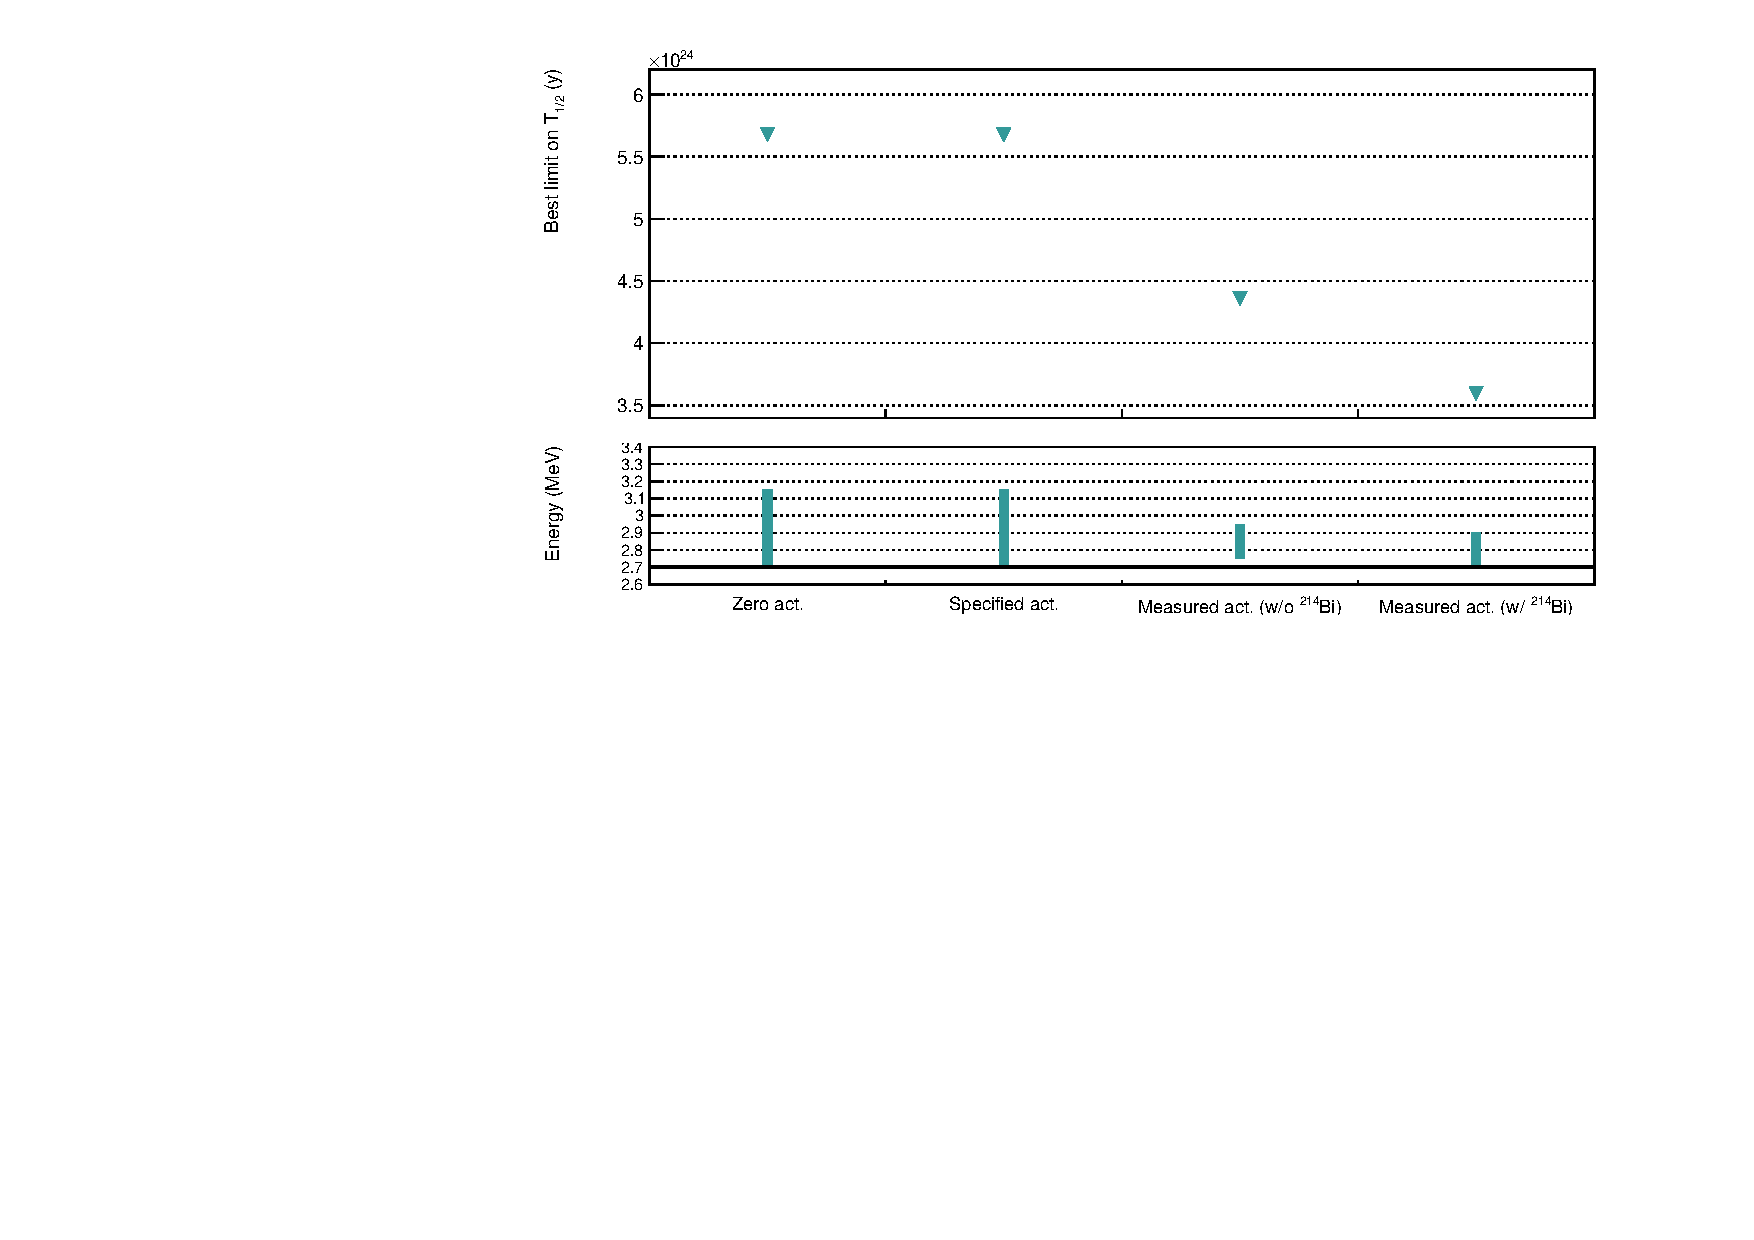
\includegraphics[width=1.1\textwidth]{Sensitivity/fig_sensitivity/contamination_level_Se_B.pdf}
  \caption{The $90\%$ CL limit on the $\zeronu$ half-life (top pad), and the corresponding ROI (bottom pad), as a function of the contamination level considered.
    For the \emph{zero activities} case, we consider hypothetical contamination levels where $\mathcal{A}^{\text{Bi}}~=~\mathcal{A}^{\text{Tl}}~=~0~$Bq/kg.
    The \emph{specified activities} are presented in Tab.~\ref{tab:real_target_act}.
    The \emph{measured activities}, provided by the BiPo detector~\cite{internal:bipo}, are presented in the same table.
    We consider successively a null \Bi\ contamination (\emph{measured act. w/o \Bi}), or equals to the $290\mu\,$Bq/kg upper limit (\emph{measured act. w/ \Bi}).
    \label{fig:real_target_act}}
\end{figure}
%% To help visualise the situation, we show in Fig.~\ref{} the distribution of $N_{0\nu}^{\text{excl.}}$, for the demonstrator case, for the two first contamination cases.
%% \begin{figure}[h!]
%%   \centering
%%   \includegraphics[width=1.1\textwidth]{Sensitivity/fig_sensitivity/}
%%   \caption{
%%     \label{fig:}}
%% \end{figure}

Tab.~\ref{tab:eff_first_order_contamination} summarises the expected number of background events for the three non-zero contamination cases presented in Fig.~\ref{fig:real_target_act}.
Regions of interest, optimised for each activity, are reminded.
For the two measured cases, both optimised regions of interest are highly reduced, especially for the case without \Bi, where the lower bound is increased from $2.7$ to $2.75$~MeV.
As this $50$~keV wide energy region is populated with a non-negligible number of background events, this change in $\text{E}_{\text{min}}$ usefully reduces the $\twonu$ background contribution, thereby limiting the increase of total expected number of background.
\begin{table}[h!]
  \centering
  \begin{tabular}{|c|c|c|c|}
    \hline
    Activity & Specified & Measured (w/o \Bi) & Measured (w/ \Bi) \\
    ROI & [$2.7$;$3.15$]~MeV & [$2.75$;$2.95$]~MeV & [$2.7$;$2.9$]~MeV \\
    \hline\hline
    $\epsilon_{0\nu}$ & $14.7$\% & $11.3$\% & $14.3$\% \\
    \hdashline
    $\twonu$  & $0.418$ & $0.122$ & $0.418$ \\
    \Tl  & $0.0475$ & $0.688$ & $0.699$ \\
    \Bi  & $0.0546$ & $0$ & $1.55$ \\
    \Rn  & $0.292$ & $0.173$ & $0.287$ \\
    Total & $0.812$ & $0.983$ & $2.95$ \\
    \hline
  \end{tabular}
  \caption{Selection efficiency of $\zeronu$ events and expected number of backgrounds events in the optimised ROI, for the exposure of the SuperNEMO demonstrator (17.5 kg.y).
    Three levels of contamination are considered.
    \label{tab:eff_first_order_contamination}}
\end{table}

The degradation of the limit on the $\zeronu$ half-life with the level of contamination remains acceptable.
However, we can try improving the situation by exploring new background rejection techniques.
This would be especially useful for the final detector case, where a slight increase in internal contaminations could be highly harmful, all the more so as the upper limit given for \Bi\ turns out to be the true contamination level.

\subsection{Optimisation of event selection}
\label{subsec:opti_ev_selection}

%% The measured level of \Tl\ isotope inside the source foils is greater than the specifications.
%% Moreover, an upper limit, higher than the specified level for SuperNEMO, has been set by the BiPo detector, regarding the internal \Bi\ level.
Following the BiPo radiopurity measurements, we wish to implement additional event selections, to reject a higher quantity of background.
Most of the double beta experiments are only sensitive to the total electron energy sum.
The unique SuperNEMO tracko-calo technology confers the experiment the ability to characterise single particles (individual energies, emission angles...).
Based on previous studies~\cite{CalvezThesis,ChaponThesis}, \emph{topological cuts}, relying on these additional observables, can be set up.
They are especially designed to reject events where the two electrons are not emitted simultaneously, or from the same location on the source foils.

\subsubsection{The internal probability}
Based on time-of-flight (TOF) computation, the internal probability (\Pint) is derived from the internal $\chi^{2}_{int}$ (see details in Sec.~\ref{subsec:analysis_tools}).
In Fig.~\ref{fig:Pint} are presented the internal probability spectra for the $\zeronu$ signal and all background processes, after the first-order selections.
These distributions are normalised to the double beta half-lives, and the nominal activities.
Equivalent distributions, but with different \Bi\ and \Tl\ contamination levels, can be derived for the case of measured activities.
The internal probability distributions for the $\zeronu$ and $\twonu$ processes follow the expected flat distribution for electrons emitted simultaneously from the source.
As internal Bismuth disintegration actually takes place inside the sources, the \Bi\ distribution is also flat.
The same could have been assumed for Thallium, however, the distribution is distorted at low internal probabilities.
This might be explained by the existence of a metastable excited state ($\tau_{1/2} = 294 ps$) of the daughter nuclei, which would slightly delay the second electron emitted via internal conversion.
This feature is addressed in detail in Chap.~\ref{ch:timediff}.
The Radon, being a non-internal background, presents a large peak at low internal probabilities.
\begin{figure}[h!]
  \centering
  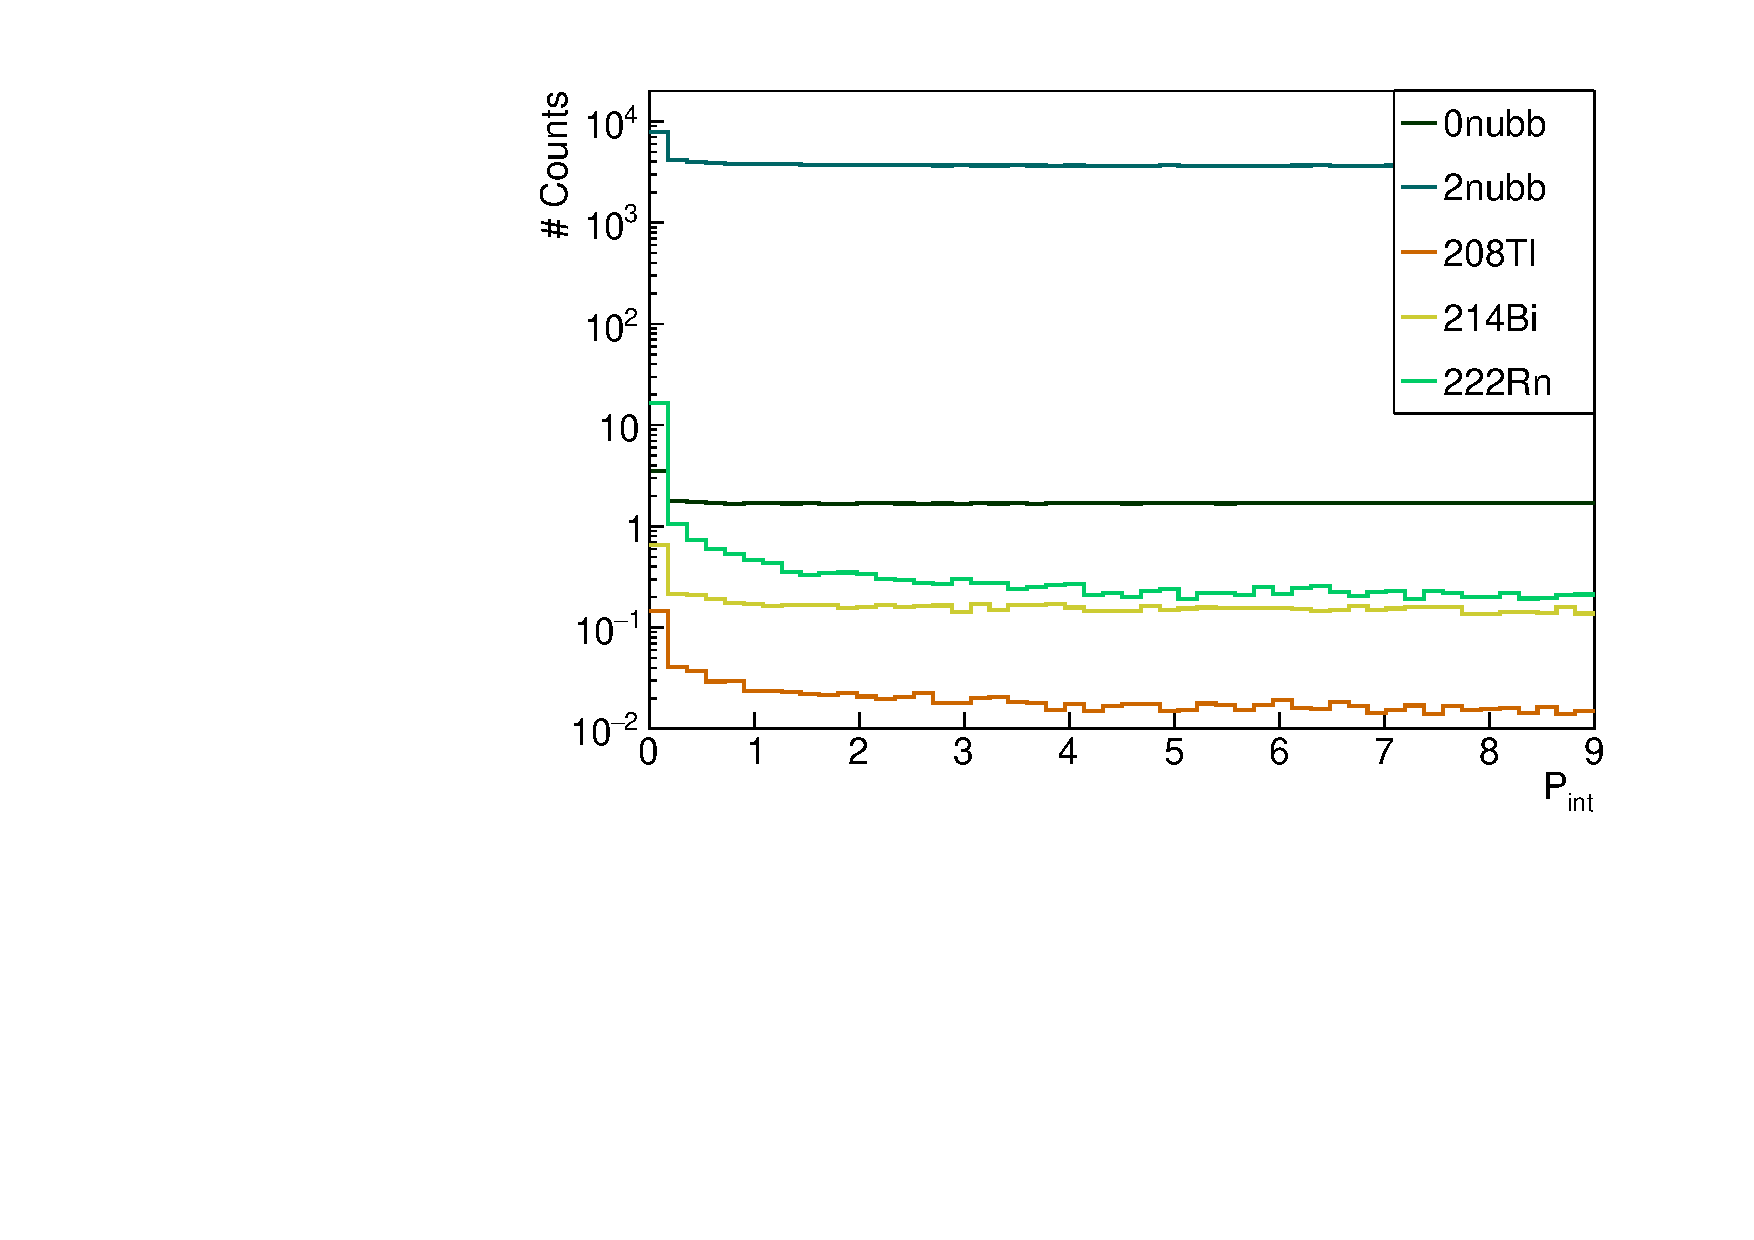
\includegraphics[width=0.85\textwidth]{Sensitivity/fig_sensitivity/InternalProbability.pdf}
  \caption{Internal probabilities for all processes.
    First-order cuts have been applied.
    $\beta\beta$ distributions are normalised to the half-lives, and background processes are normalised to the specified activities.
    \label{fig:Pint}}
\end{figure}

We want to evaluate the influence of a cut-off on the simulations using internal probability as a rejection criterion: simulated events are selected only if their \Pint\ value is upper than a given limit.
The standard value applied in NEMO-$3$ analyses was \Pint~$>~4~\%$.
We wish to establish the most adequate \Pint\ selection level for the SuperNEMO demonstrator.
To do so, we vary the \Pint\ minimal value applied on simulations, and for each we evaluate the limit reached on $\Tbeta$ (at a $90$~\% confidence interval), as well as the optimised ROI.
The best internal probability cut-off value to be applied is the one maximising this sensitivity, and is specific for each contamination level.

We depict in Fig.~\ref{fig:cont_Pint} a set of four figures that help to better understand this optimisation.
We consider two levels of contamination, the specified and measured contamination levels (taking the upper limit for \Bi).
We first detail these figures for the case of the specified activities and then explain what we observe for the measured activities.
\begin{figure}[!h]
\centering
\begin{subfigure}[t]{0.49\textwidth}
  \centering
  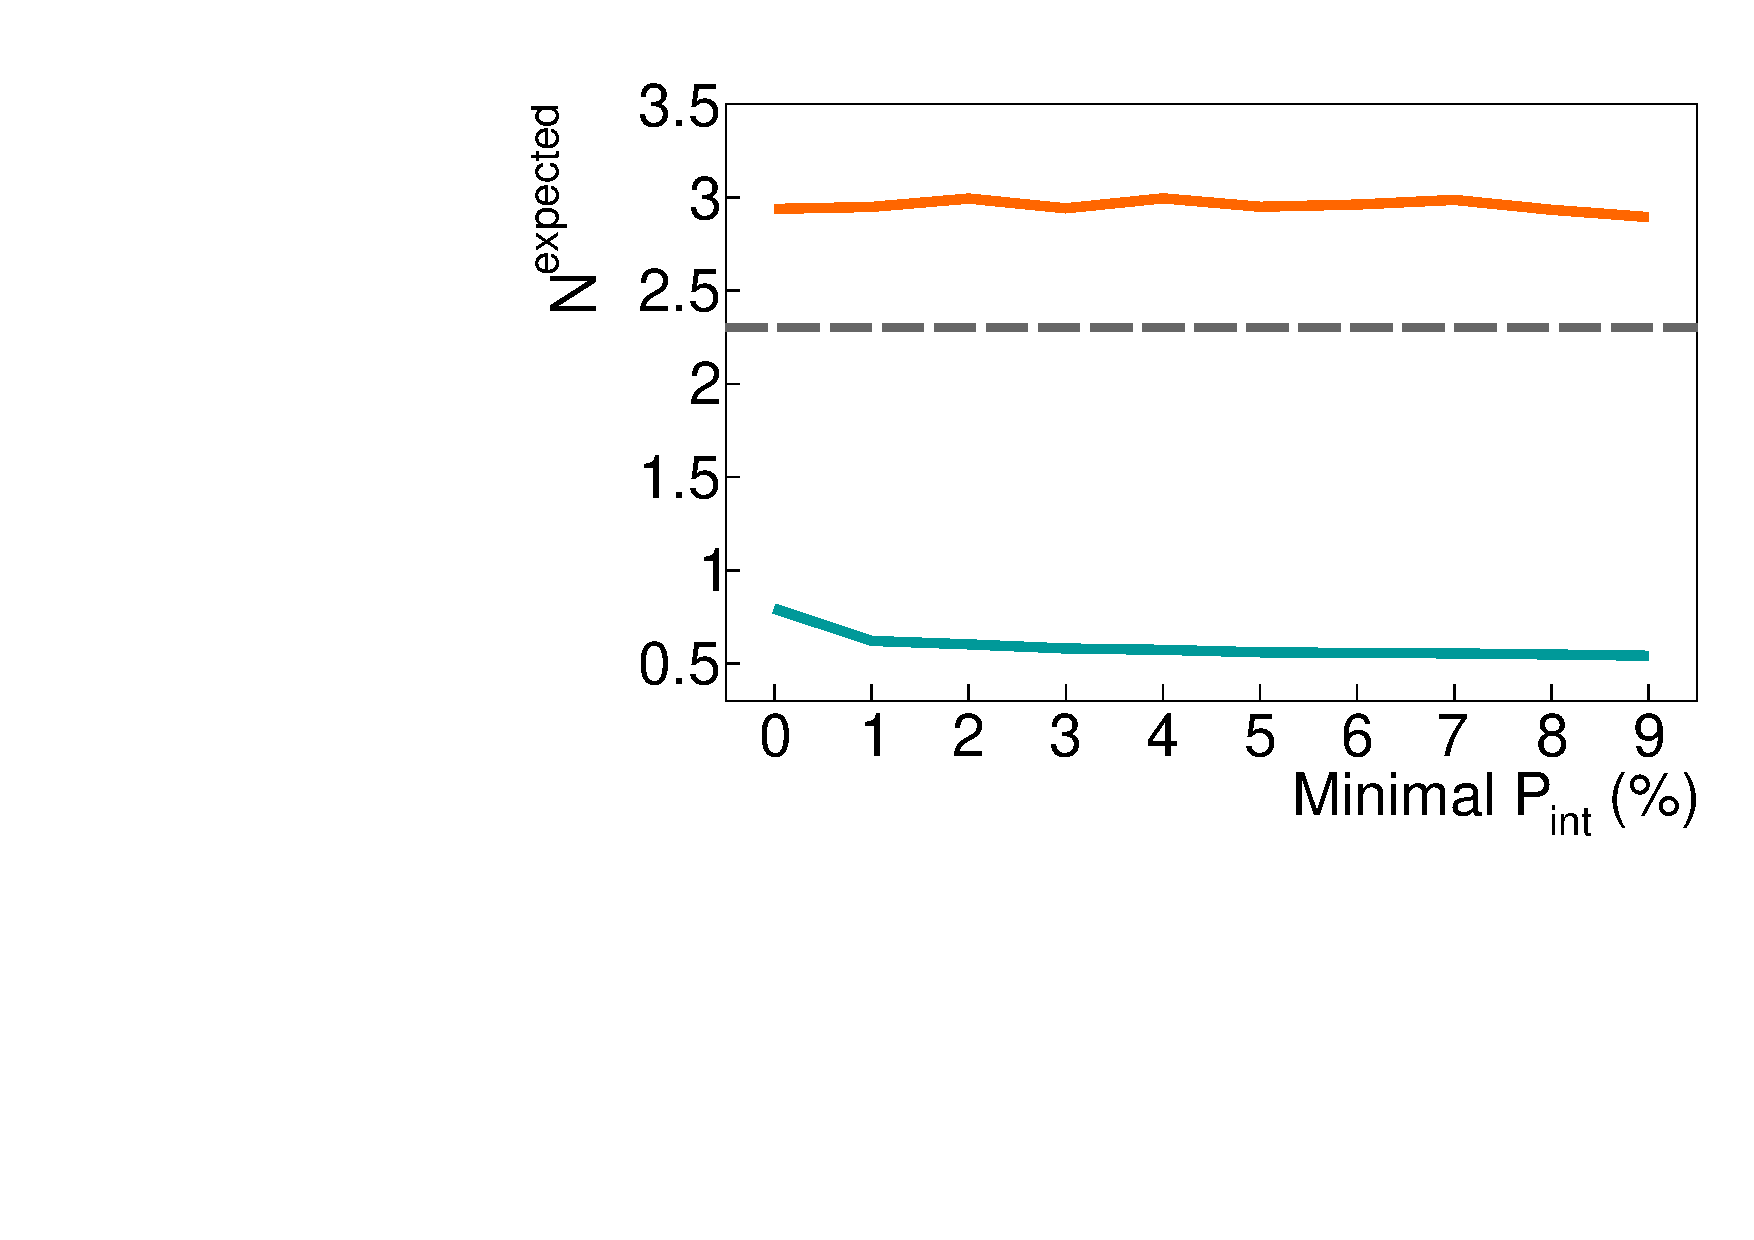
\includegraphics[width=0.9\textwidth]{Sensitivity/fig_sensitivity/82Se_cont_cut_nexcl_B.pdf}
  \captionsetup{justification=centering}
  \caption{Total expected number of background in ROI.
    \label{subfig:cont_Pint_Nexp}}
\end{subfigure}
\hfill
\begin{subfigure}[t]{0.49\textwidth}
  \centering
  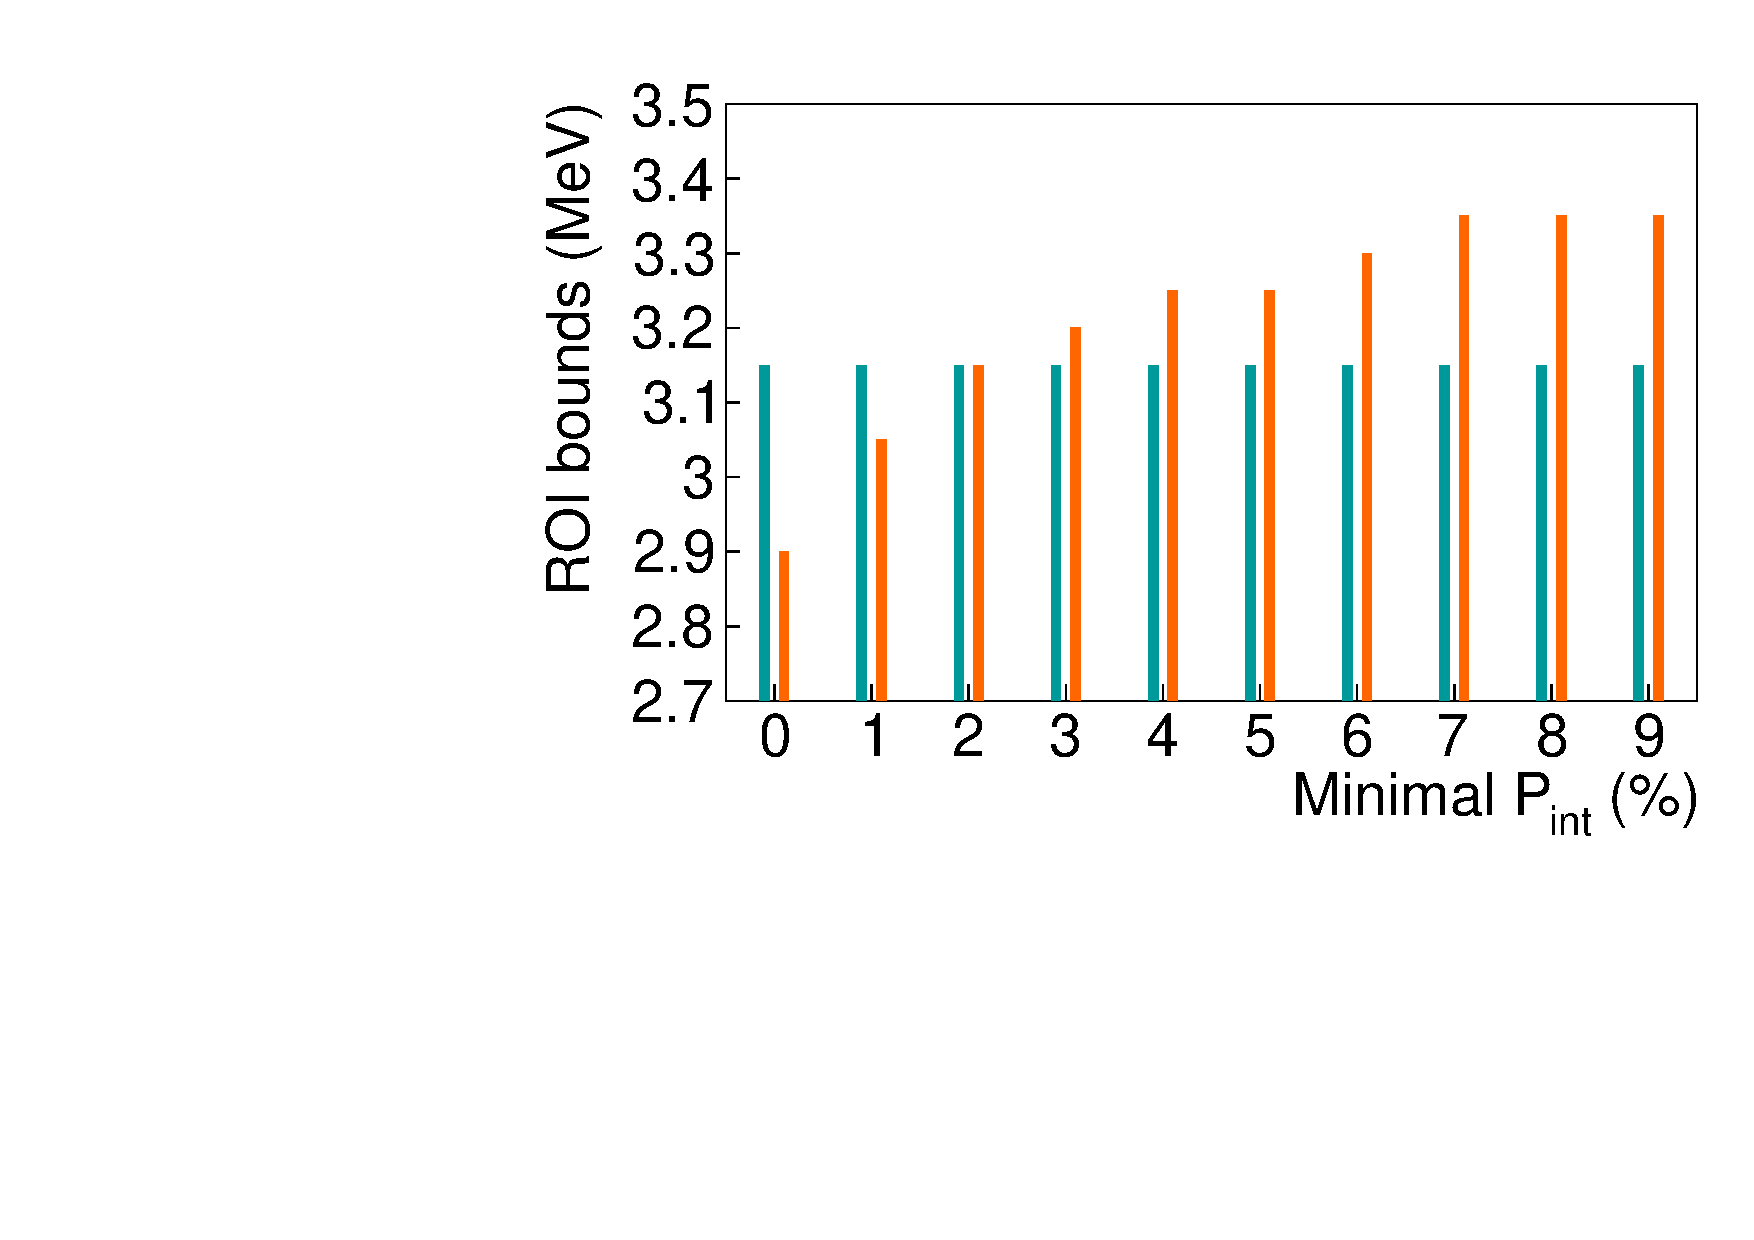
\includegraphics[width=0.9\textwidth]{Sensitivity/fig_sensitivity/ROI_cut_Pint_B.pdf}
  \captionsetup{justification=centering}
  \caption{ROI optimisation.
    \label{subfig:cont_Pint_ROI}}
\end{subfigure}
\vskip\baselineskip
\begin{subfigure}[t]{0.49\textwidth}
  \centering
  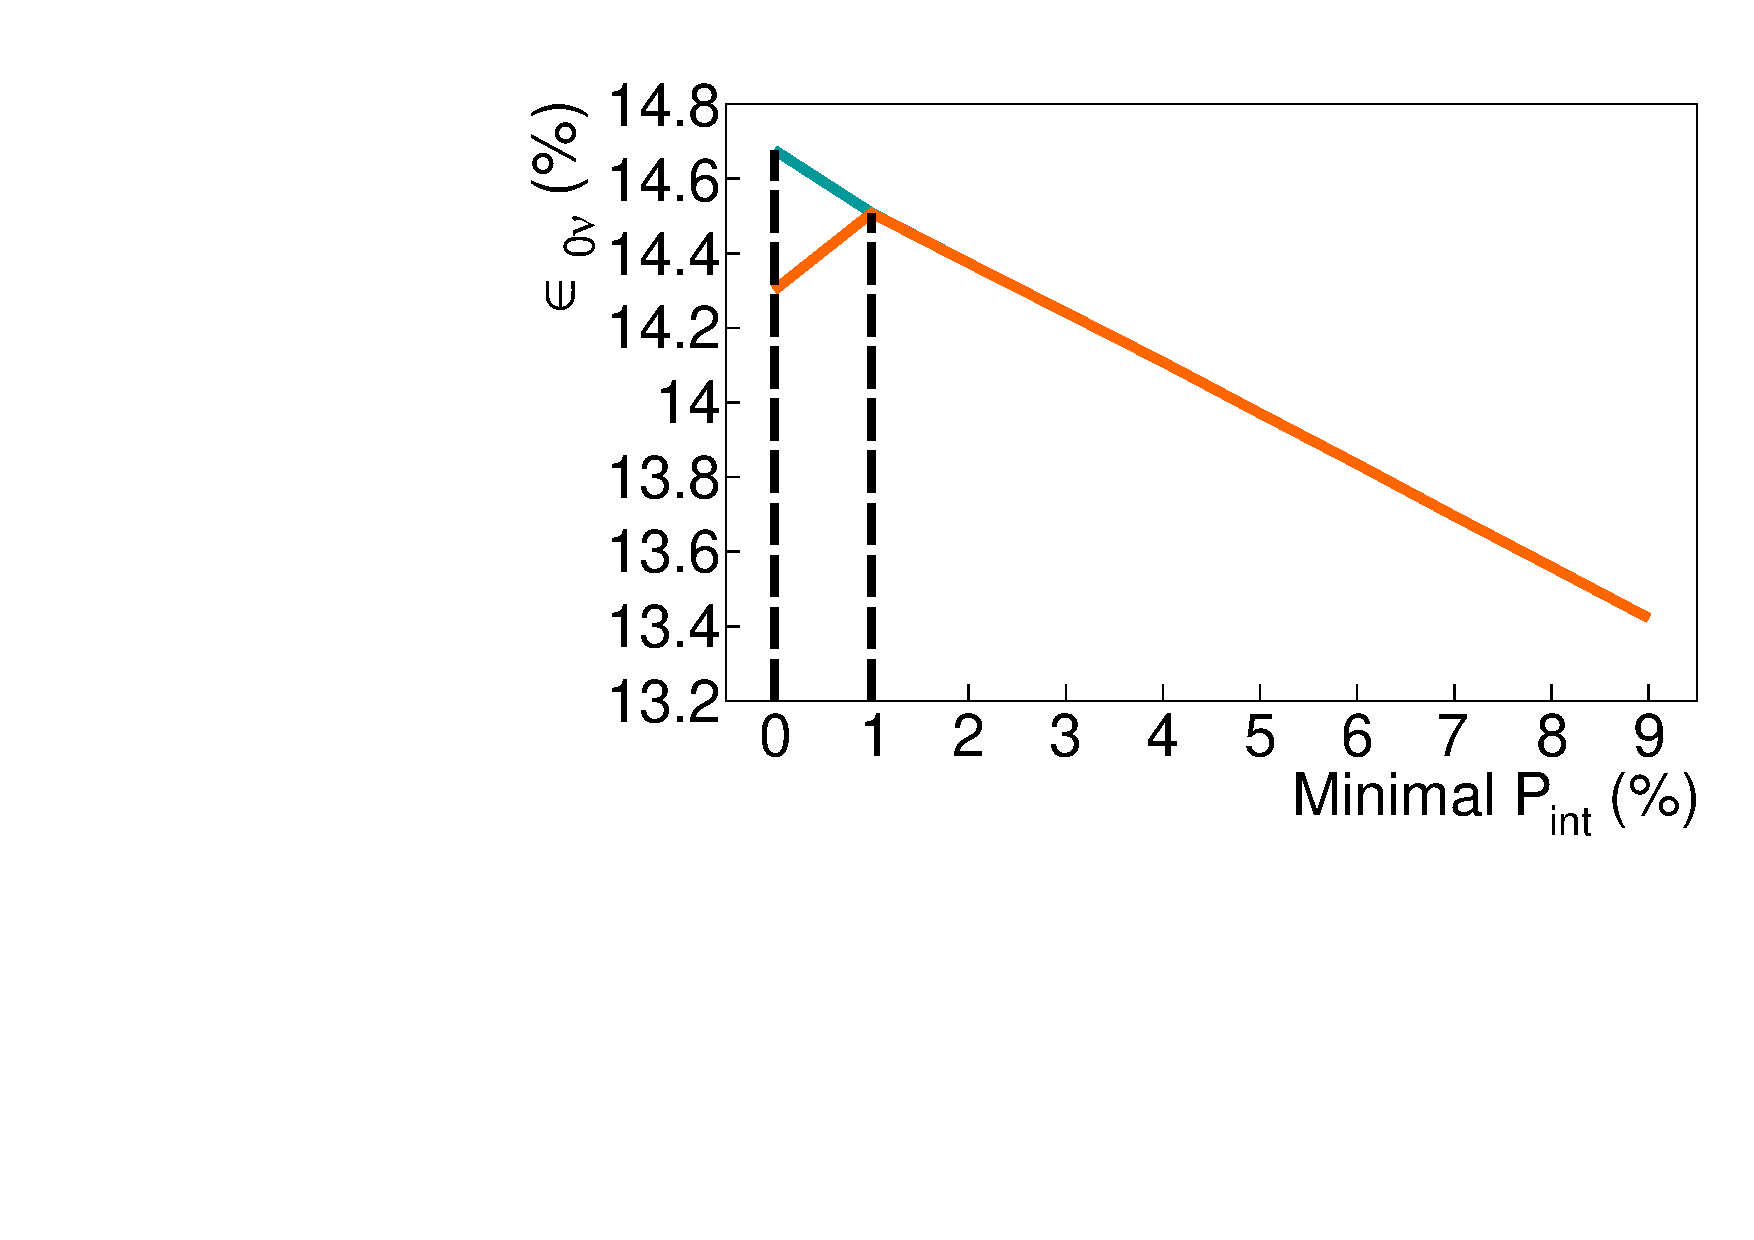
\includegraphics[width=0.9\textwidth]{Sensitivity/fig_sensitivity/cont_cut_eff_B.pdf}
  \captionsetup{justification=centering}
  \caption{$\zeronu$ selection efficiency in ROI.
    \label{subfig:cont_Pint_eff}}
\end{subfigure}
\hfill
\begin{subfigure}[t]{0.49\textwidth}
  \centering
  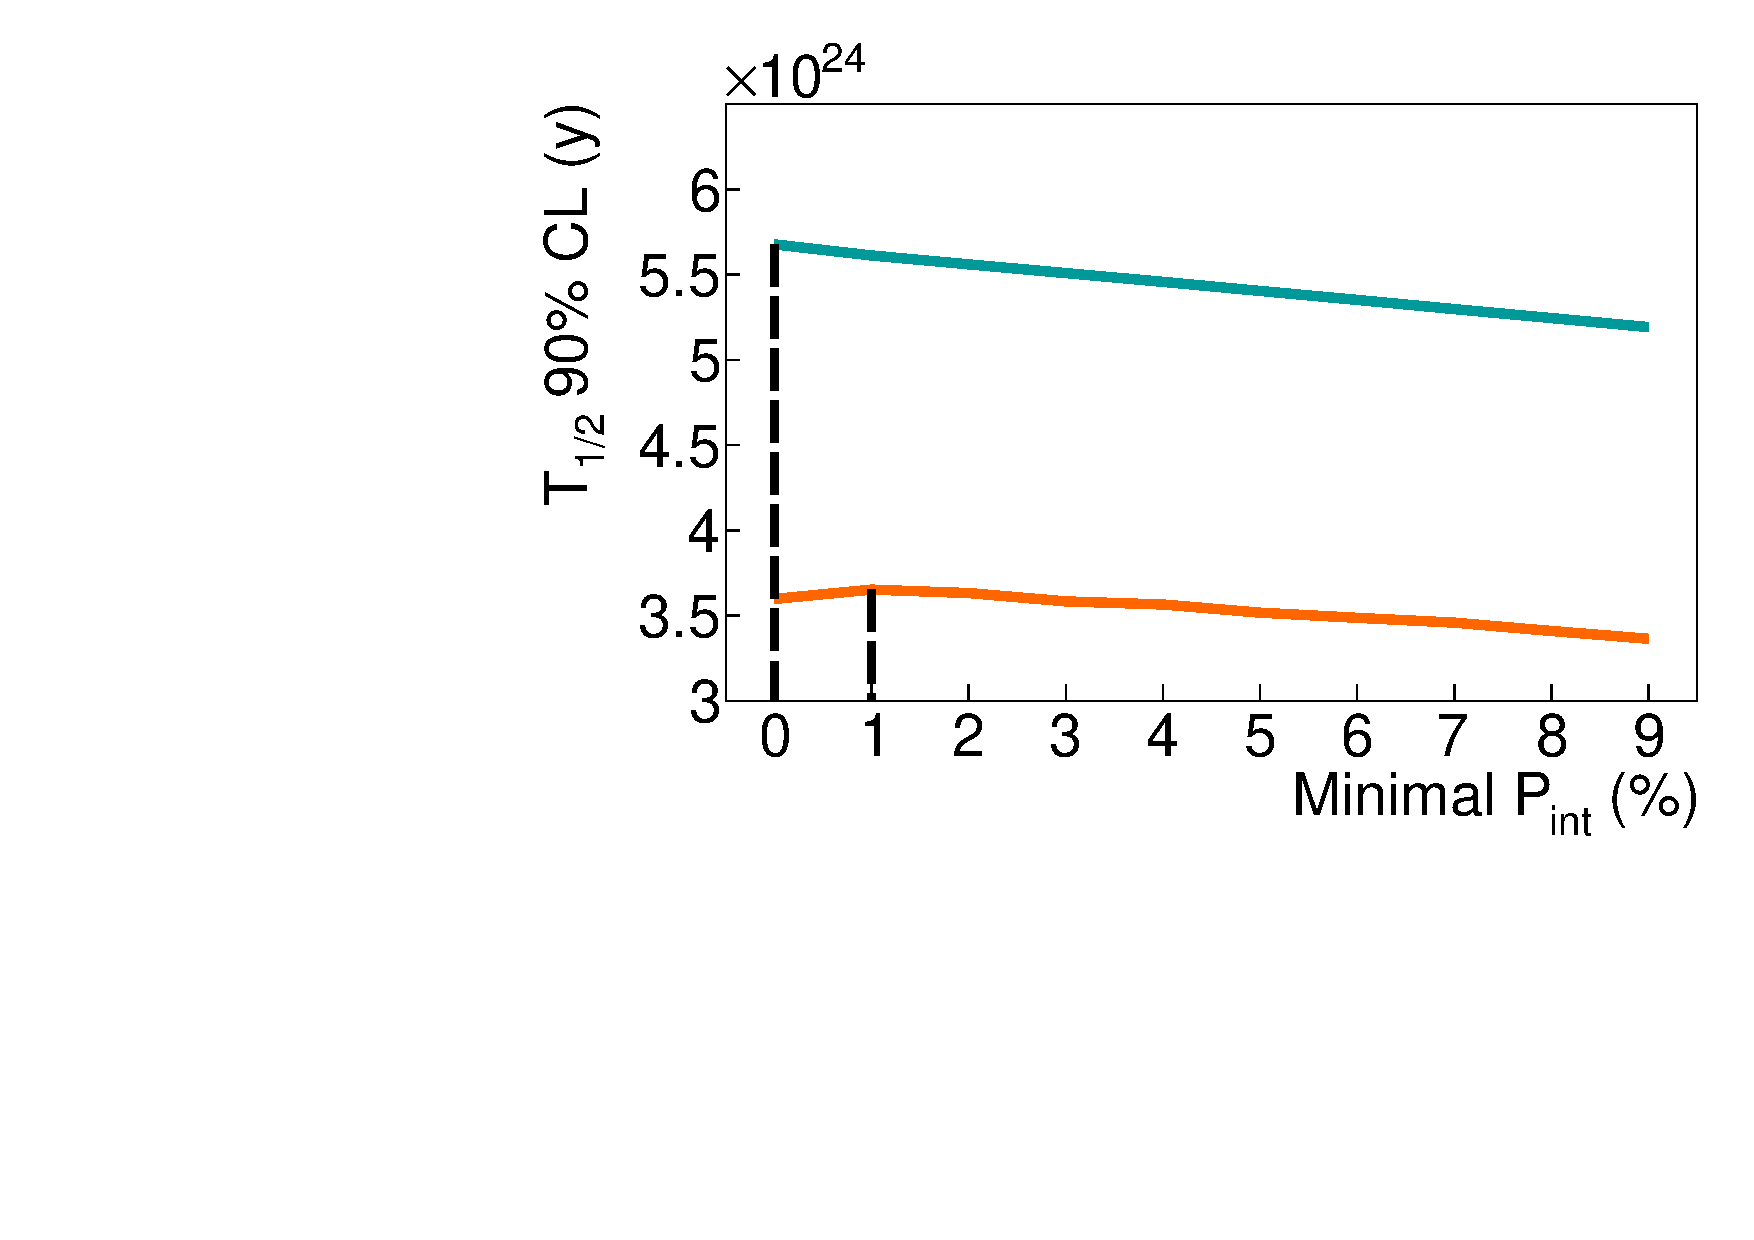
\includegraphics[width=0.9\textwidth]{Sensitivity/fig_sensitivity/cont_cut_T12_B.pdf}
  \captionsetup{justification=centering}
  \caption{Limit on $\Tbeta$.
    \label{subfig:cont_Pint_T12}}
\end{subfigure}
\vskip\baselineskip
\begin{subfigure}[t]{0.49\textwidth}
  \centering
  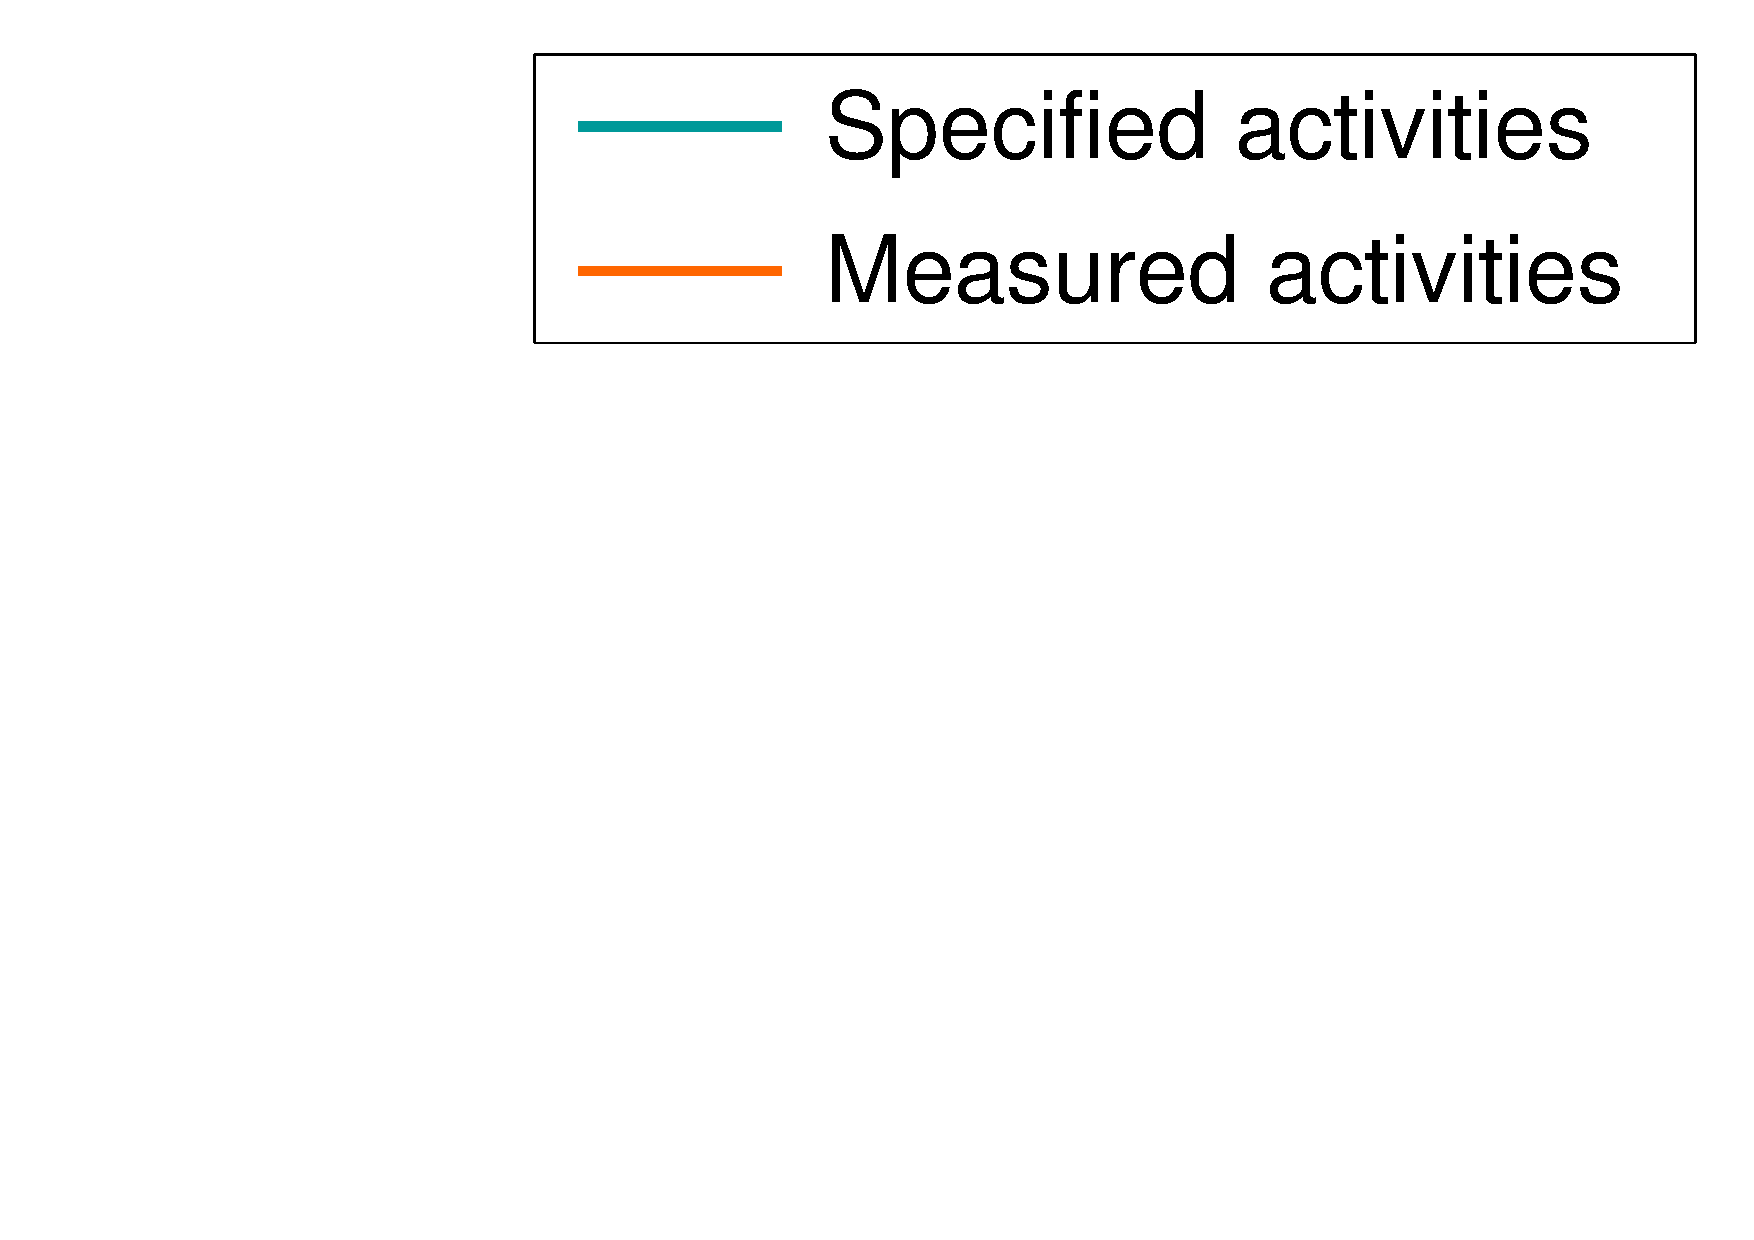
\includegraphics[width=0.5\textwidth]{Sensitivity/fig_sensitivity/legend_cut_Pint.pdf}
  \end{subfigure}
\caption{Total number of expected background in ROI (a),
  evolution of the regions of interest (b),
  $\zeronu$ selection efficiency in ROI (c),
  and limit set on $\Tbeta$ at $90\%$ CL (d),
  as a function of the cut-off applied on internal probability, \Pint.
  The ROI is optimised for each \Pint\ value.
  Results are displayed for two contamination levels: the specified (blue) and the measured (orange) activities (taking into account the upper limit provided for \Bi).
  An exposure of $17.5$~kg.y is considered.
  Two vertical dashed lines in (c) and (d) display the best \Pint\ selections to be applied in order to improve the $\Tbeta$ sensitivity of the experiment.
  \label{fig:cont_Pint}}
\end{figure}

\paragraph{Specified activities}
The total expected number of background in the ROI (Fig.~\ref{subfig:cont_Pint_Nexp}) is very low compared to one: it is smaller than $0.8$ for \Pint$>0$\%, and slightly decreases when the minimal cut on \Pint\ increases.
Therefore, the number of excluded signal events, $N_{0\nu}^{\text{excl.}}$, is set to its minimal value of $2.303$, regardless of the \Pint\ level.
As a consequence, the ROI bounds are stable (Fig.~\ref{subfig:cont_Pint_ROI}) and thus $\epsilon_{0\nu}$ is only impacted by the \Pint\ level applied which makes it decrease (Fig.~\ref{subfig:cont_Pint_eff}).
All these observations allow to understand the evolution of $\Tbeta$ (Fig.~\ref{subfig:cont_Pint_T12}), decreasing with the \Pint\ level applied on simulations.
The sensitivities displayed for a $0\%$ cut-off on P$_{\text{int}}$ of course correspond to the results given in Fig.~\ref{fig:real_target_act}.

\paragraph{Measured activities}

The total number of expected background event in the ROI is higher than for the specifications.
Nevertheless, this level is too low for the \Pint\ cut-off to have an impact on it, and the number of expected background remains globally constant.
When the minimal acceptable \Pint\ is changed from $0$ to $1$~\%, the ROI upper bound increases from $2.9$ to $3.05$~MeV.
Usually, the variation of this bound does not have such a great impact on the event selection.
Nevertheless, in the measured activities case, for a \Pint~$>~0~\%$ level, the ROI is optimised at the narrow [$2.7$;$2.9$]~MeV interval, where the upper bound is located in an energy region still populated by signal.
Therefore, even small variations of this upper bound has a great impact on the $\zeronu$ selection efficiency, explaining its local increase for \Pint\ cut-off between $0$ and $1$\%.
For \Pint\ selections greater than $1~\%$, we come back in cases where the upper bound of the ROI no longer has an impact on $\epsilon_{0\nu}$.
At this level, only variations of the total number of background events have an impact.
As the limit set on $\Tbeta$ depends directly on $\epsilon_{0\nu}$, the variations presented in Fig.~\ref{subfig:cont_Pint_eff} fully explain the results displayed in Fig.~\ref{subfig:cont_Pint_T12}, presenting the evolution of $\Tbeta$ with the internal probability selection level.

The optimisation work we have just presented is of interest in the case of measured activities, where the cut-off on \Pint\ is set at $1$\%.
We will see in the following sections that this optimisation is also be useful, especially when studying the influence of the magnetic field.
However, this rejection criterion has only a limited impact on the improvement of $\Tbeta$ sensitivity for the specified activities, because of the very low contamination levels considered.
Indeed, paradoxically, the selection on internal probability worth it only if there is enough background events to be rejected, as we can start observing for the measured activities case.
Nevertheless, in that case, we recommend to keep at least a loose cut-off at \Pint$>4~\%$.
Indeed, this only slightly degrades the sensitivity (around $4$\%) while insuring the rejection of potential harmful external backgrounds for a more general study.



\subsubsection{Vertices distance}

NEMO-$3$ analyses also used the distance between the reconstructed vertices on the source foils as a background rejection criterion.
As we have shown that the additional \Pint\ cut-off is poorly adapted for the low activities of SuperNEMO sources, it is interesting to know if we can improve the results by using this second selection.
Thanks to the trajectory fitting algorithm, we have access to the ($Y,Z$) coordinates of the latter, and by extension, to the distance between them.
In the previous studies, the choice was made to look at the effect of this selection, separately on the $Y$ (perpendicular to the wires) and $Z$ (parallel to the wires) directions.
We choose to follow the same approach, and we give the results for a cut along the $Z$ axis, but the conclusions remain valid for the $Y$ direction.
Fig.~\ref{fig:vertex_dist} shows the distributions of the absolute value of the distance between foil vertices for each process studied.
We would use this information in order to maximise the double $\beta$ decays to be selected, while rejecting natural isotope disintegrations.
\begin{figure}[h!]
  \centering
  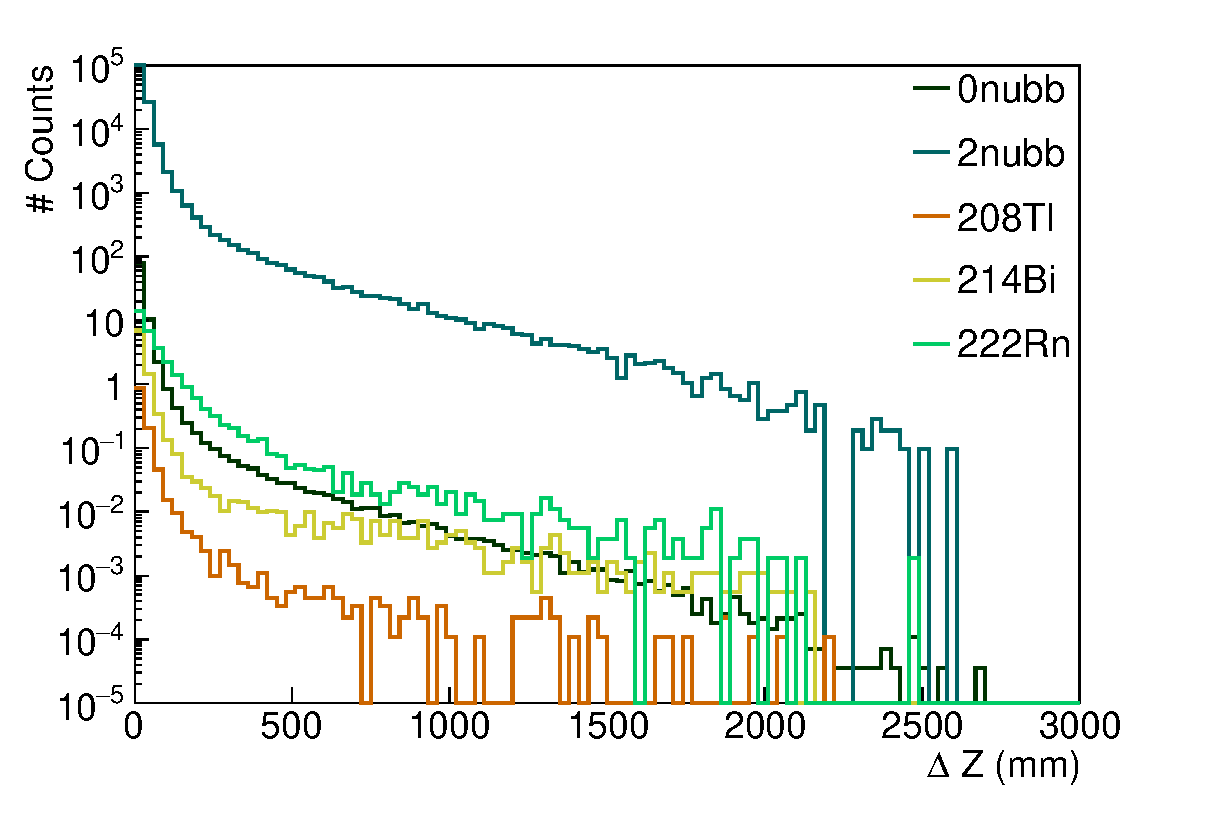
\includegraphics[width=0.8\textwidth]{Sensitivity/fig_sensitivity/Vertex_distance.eps}
  \caption{Distance along the $Z$ direction between the vertices of the $2$ reconstructed electrons, for each process considered.
    The $\twonu$ spectrum is normalised to $\Ttwonu~=~9.39\times~10^{19}$~y, and \Tl, \Bi\ and \Rn\ backgrounds are normalised to the nominal activities.
    The amplitude of the $\zeronu$ is arbitrarily set at the $90$\% limit obtained with NEMO-$3$.
    No energy cut is applied.
    \label{fig:vertex_dist}}
\end{figure}

In the same way as the previous paragraph, Fig.~\ref{fig:cont_vertex} displays all informations leading to the maximisation of $\Tbeta$, allowing to study the impact of the vertices distance cut-off on the final sensitivity.
Overall, these figures show us that too strict cut-off on the distance between vertices would lead to a decrease in sensitivity.
Because of the variations of the $\zeronu$ selection efficiency and the total number of background events, the $\Tbeta$ distributions reaches a plateau, corresponding to the sensitivities achieved with the first-order cuts and optimised \Pint.
In practice, as it is done for \Pint, a selection on vertex distance will always be applied, even if it is very loose, as such a cut-off could be useful for rejecting unexpected background (coincidence between independent events, for instance).
We recommend to apply a loose cut-off level at $|~\Delta Z~|~<~80$~mm, which does not degrade significantly the sensitivity.
The same conclusions apply to the $|~\Delta Y~|$ cut-off.
\begin{figure}[!h]
\centering
\begin{subfigure}[t]{0.49\textwidth}
  \centering
  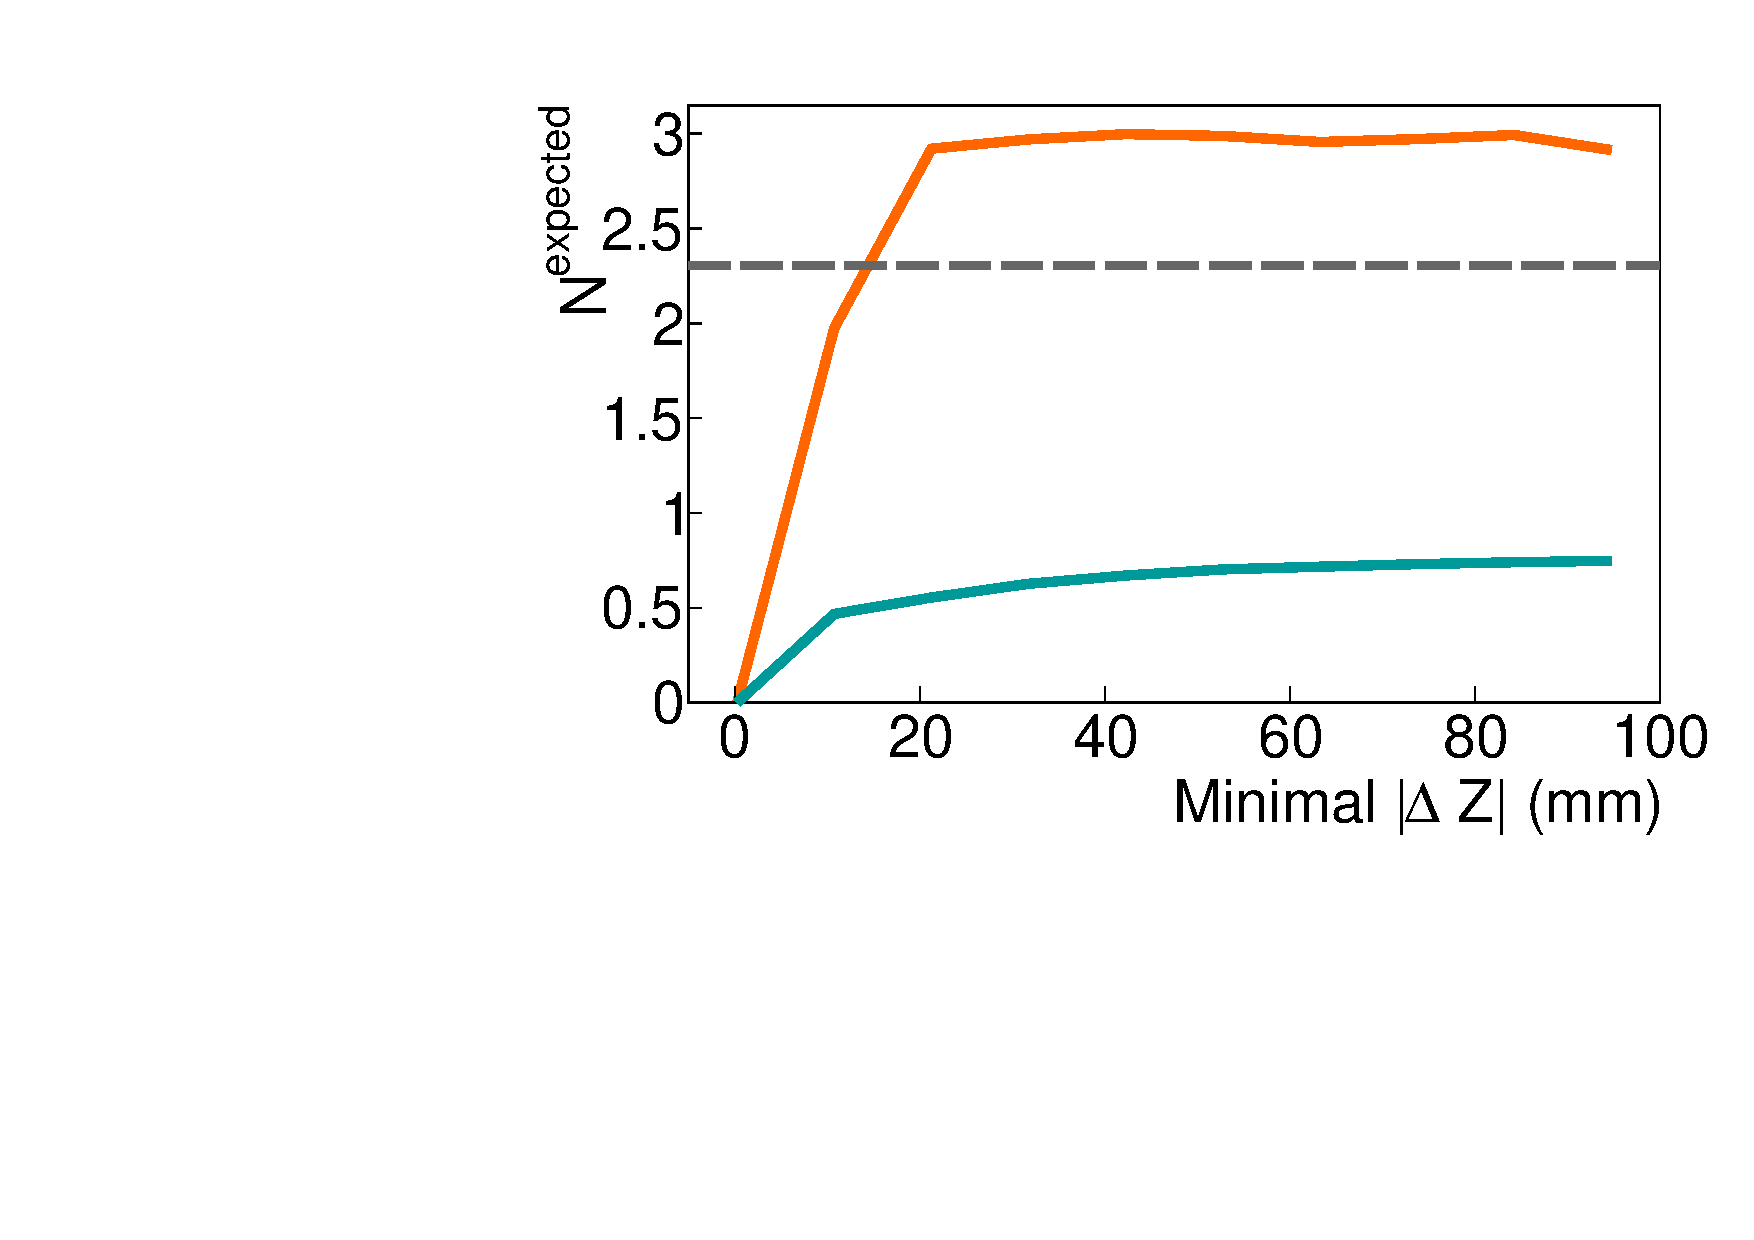
\includegraphics[width=0.9\textwidth]{Sensitivity/fig_sensitivity/82Se_cont_cut_vertex_nexcl_B.pdf}
  \captionsetup{justification=centering}
  \caption{Total expected number of background.
    \label{subfig:cont_vertex_Nexp}}
\end{subfigure}
\hfill
\begin{subfigure}[t]{0.49\textwidth}
  \centering
  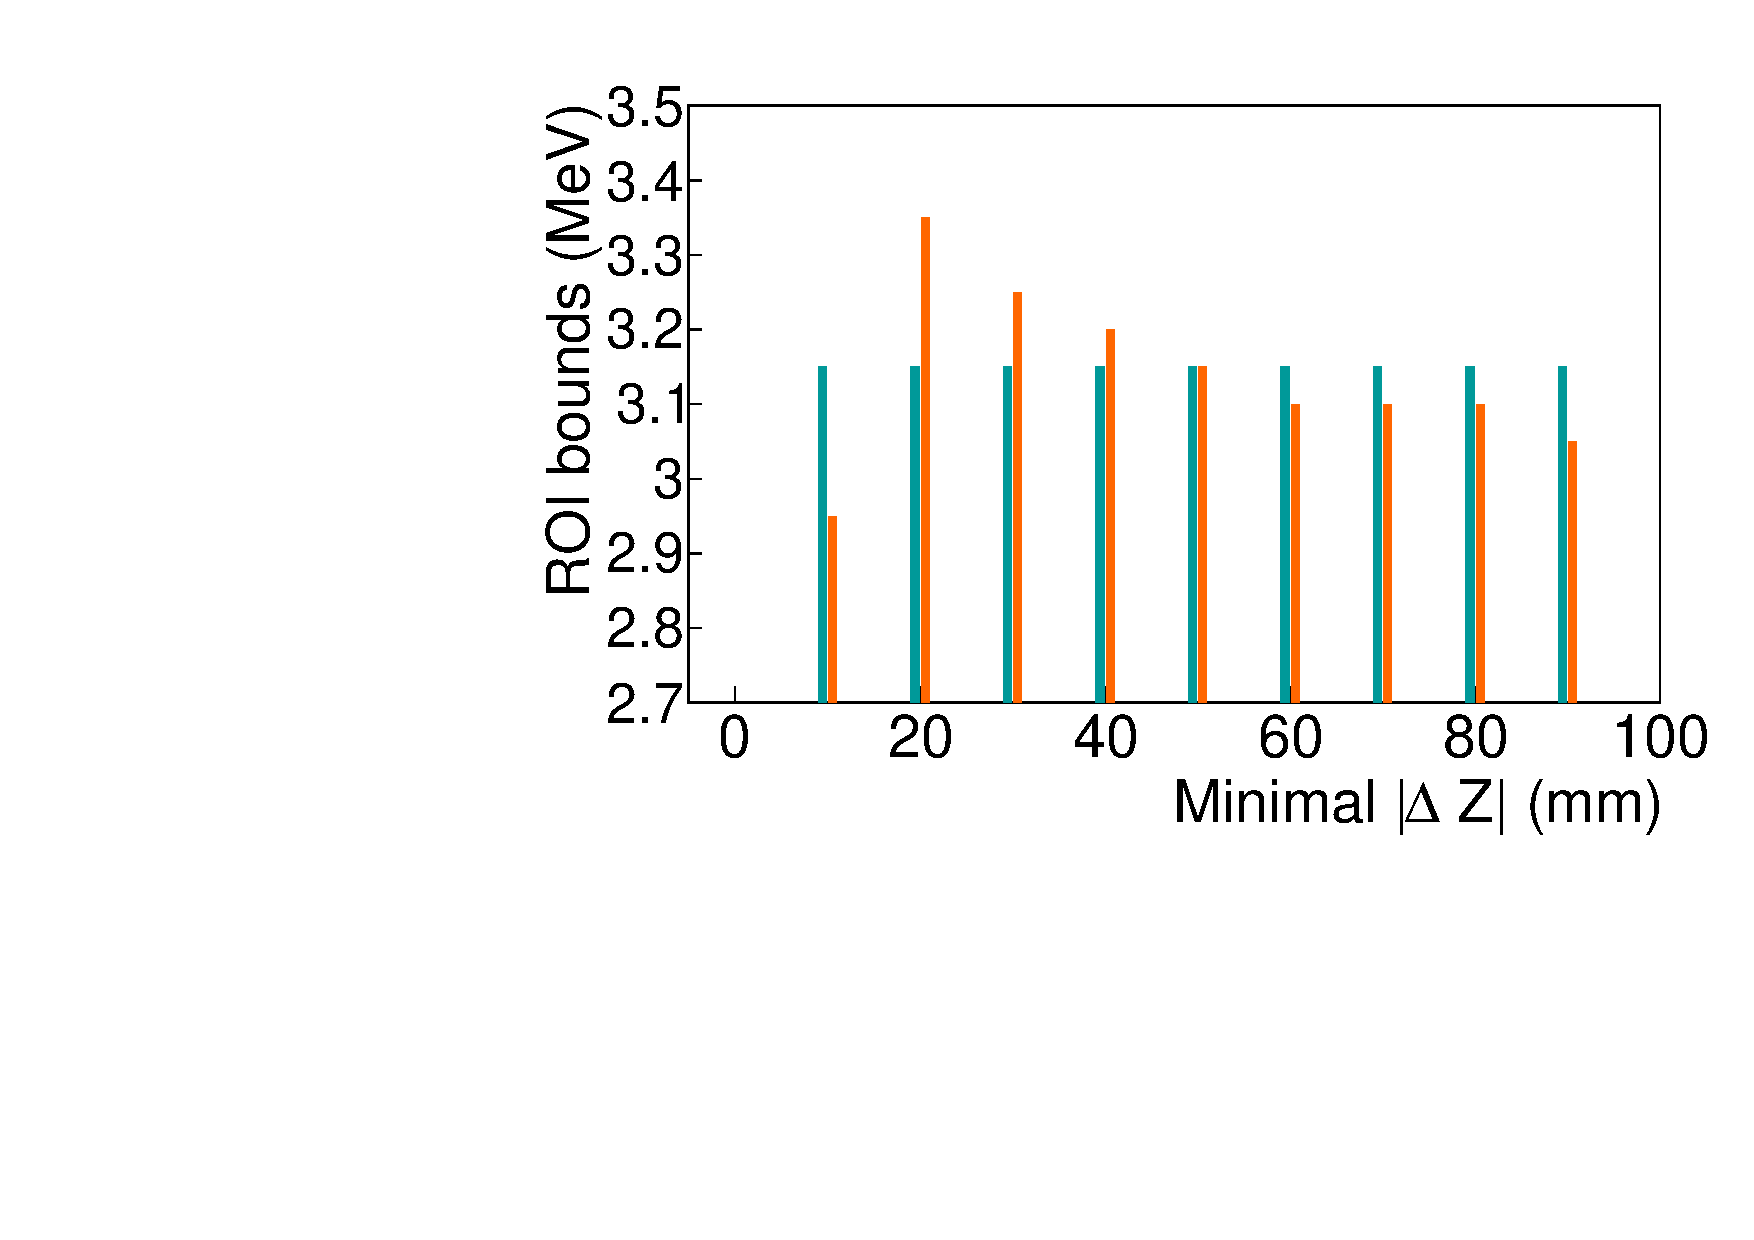
\includegraphics[width=0.9\textwidth]{Sensitivity/fig_sensitivity/82Se_ROI_cut_vertex_B.pdf}
  \captionsetup{justification=centering}
  \caption{ROI optimisation.
    \label{subfig:cont_vertex_ROI}}
\end{subfigure}
\vskip\baselineskip
\begin{subfigure}[t]{0.49\textwidth}
  \centering
  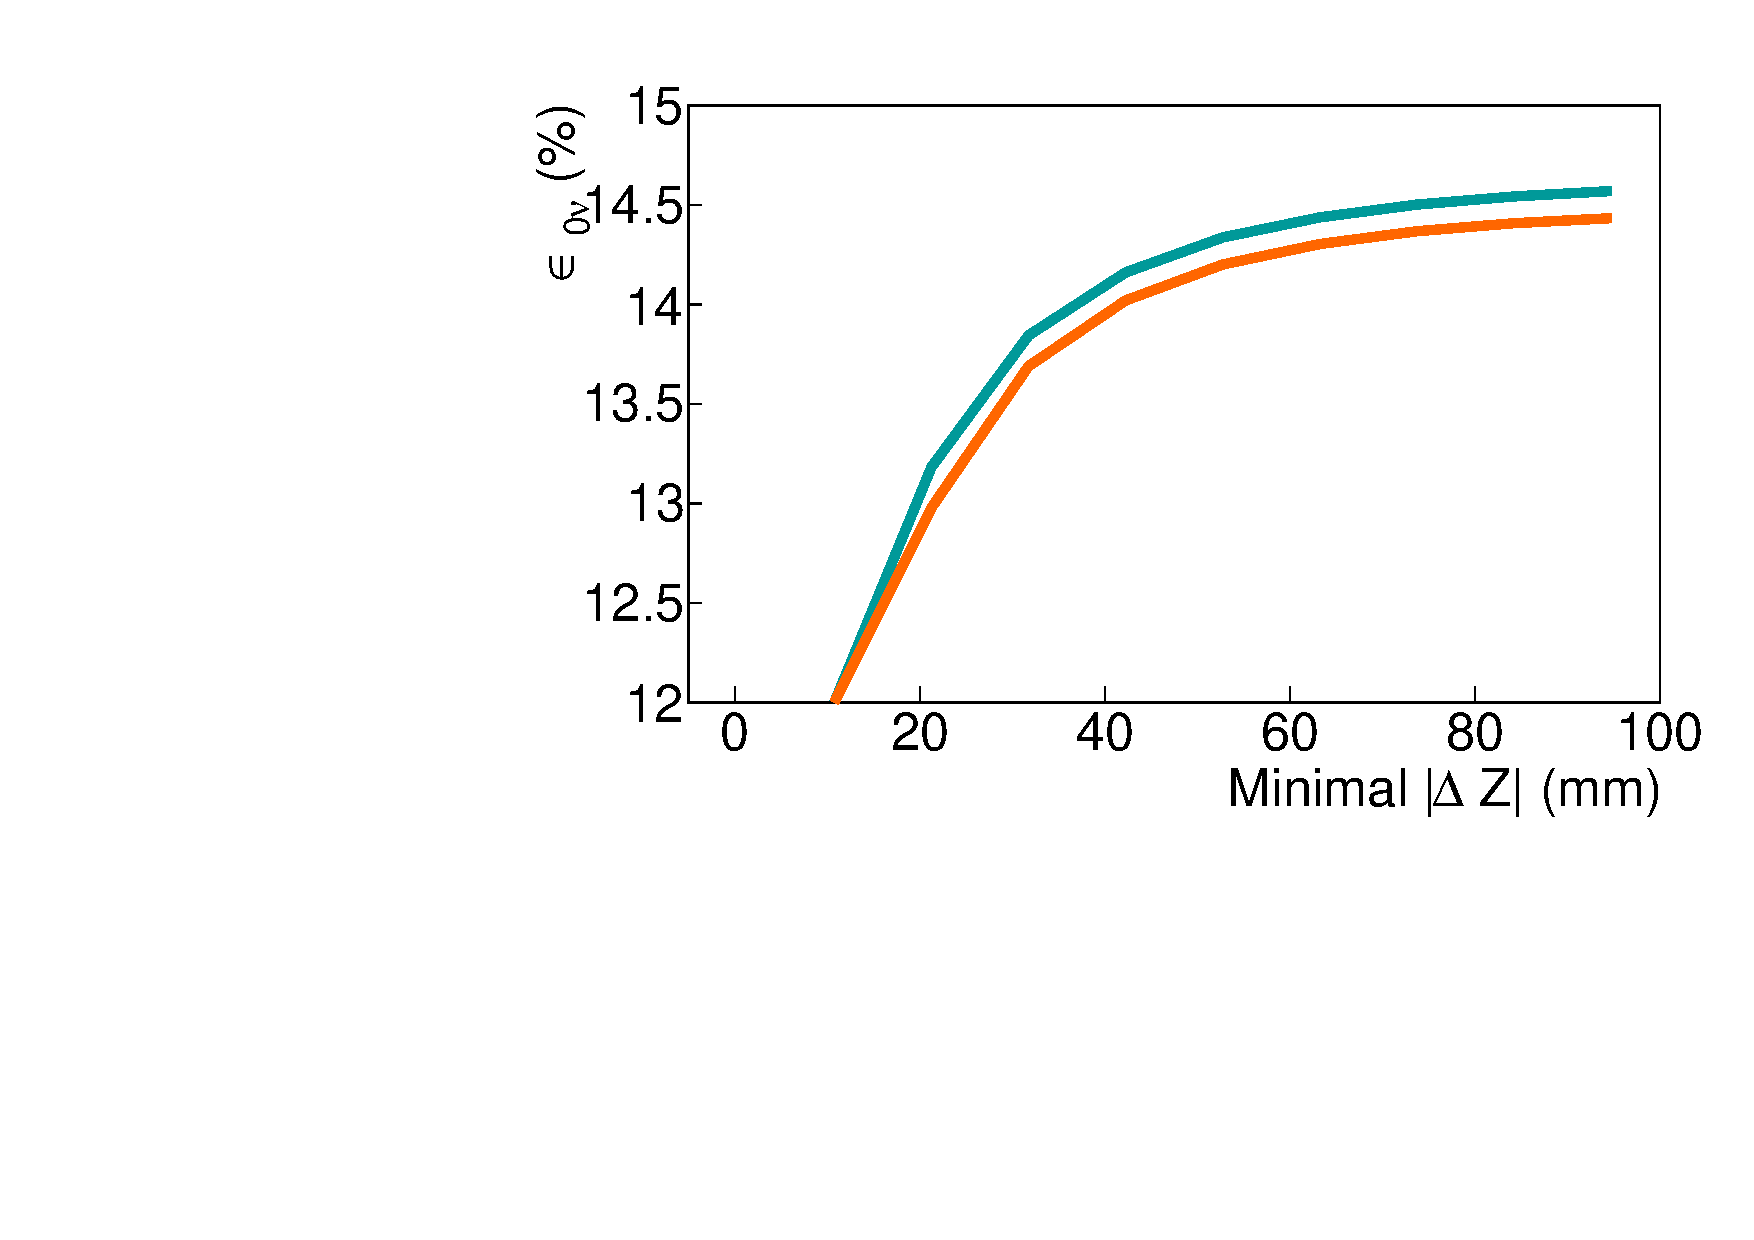
\includegraphics[width=0.9\textwidth]{Sensitivity/fig_sensitivity/82Se_cont_cut_vertex_eff_B.pdf}
  \captionsetup{justification=centering}
  \caption{$\zeronu$ selection efficiency.
    \label{subfig:cont_vertex_eff}}
\end{subfigure}
\hfill
\begin{subfigure}[t]{0.49\textwidth}
  \centering
  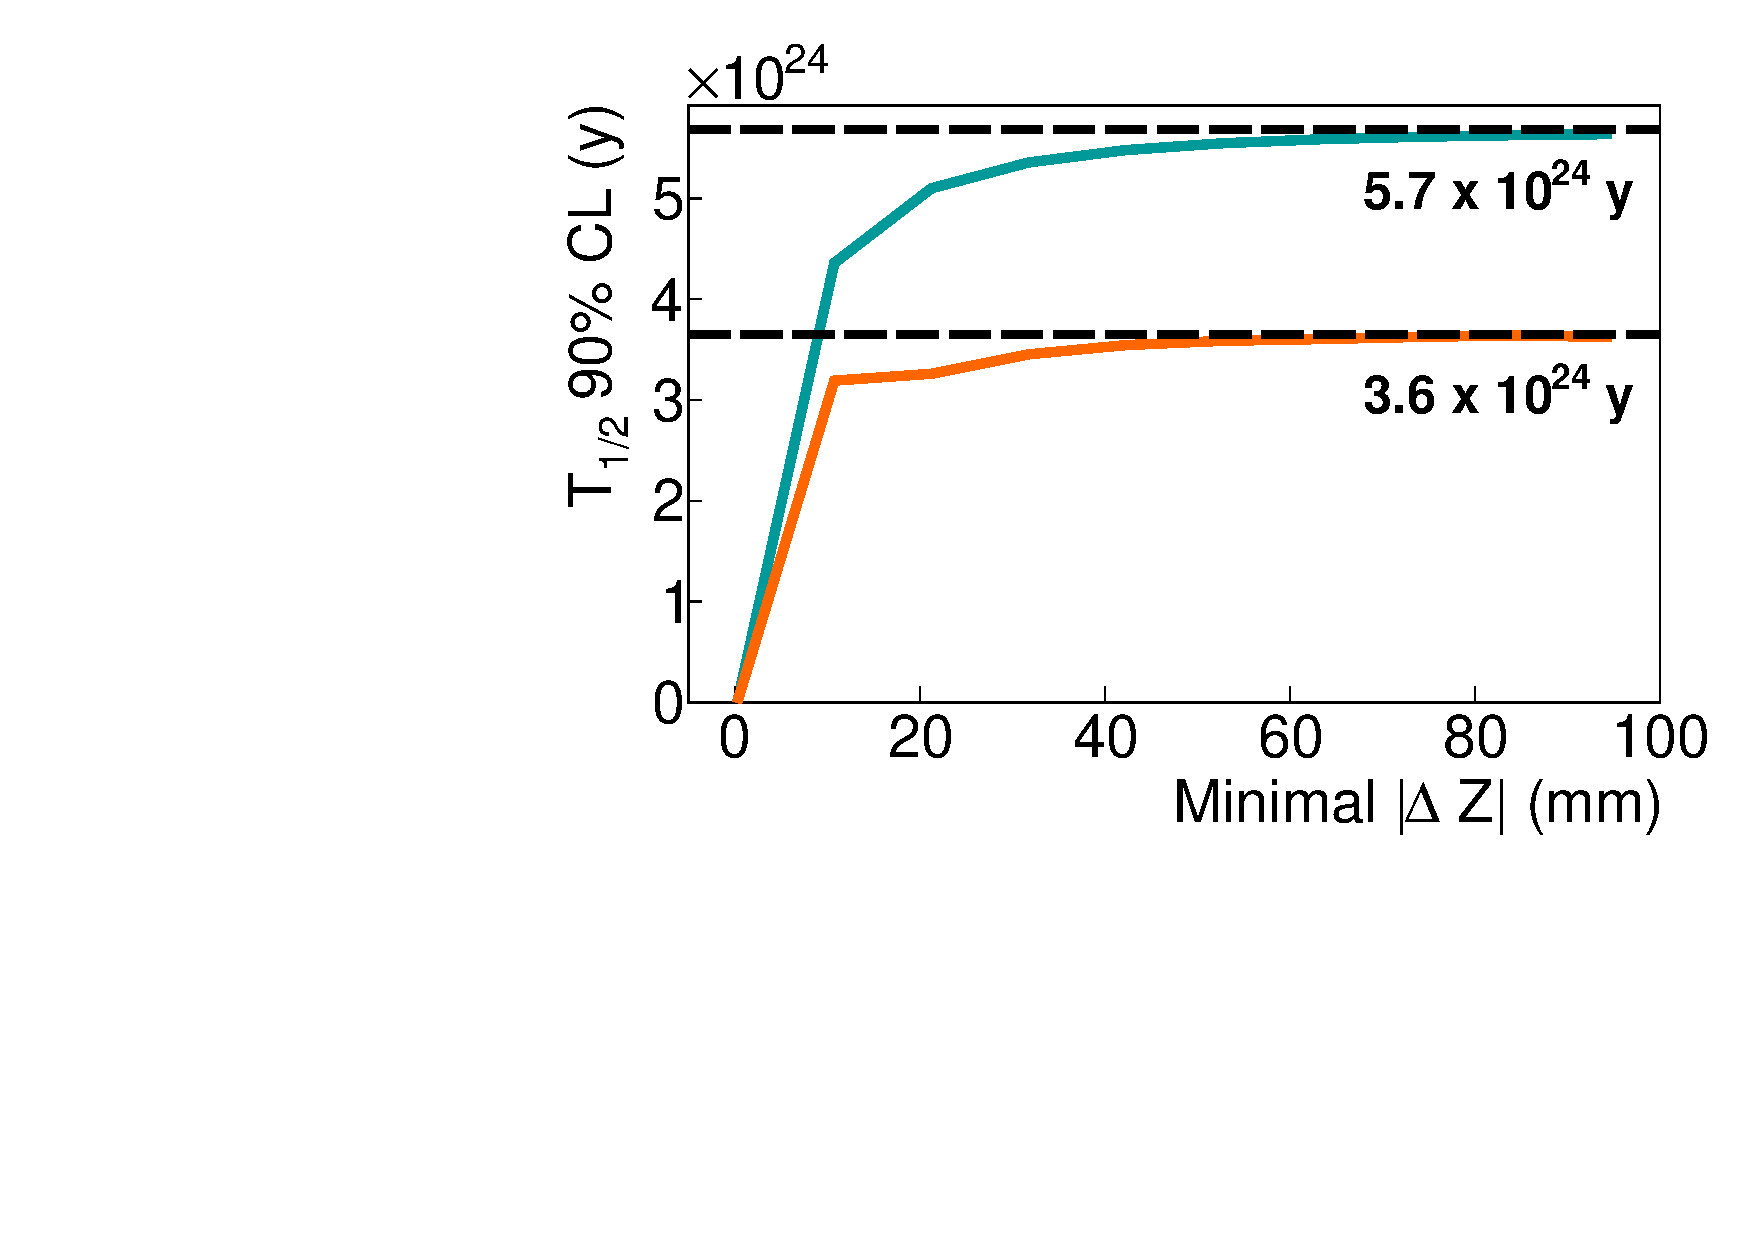
\includegraphics[width=0.9\textwidth]{Sensitivity/fig_sensitivity/82Se_cont_cut_vertex_T12_B.pdf}
  \captionsetup{justification=centering}
  \caption{Limit on $\Tbeta$.
    \label{subfig:cont_vertex_T12}}
\end{subfigure}
\vskip\baselineskip
\begin{subfigure}[t]{0.49\textwidth}
  \centering
  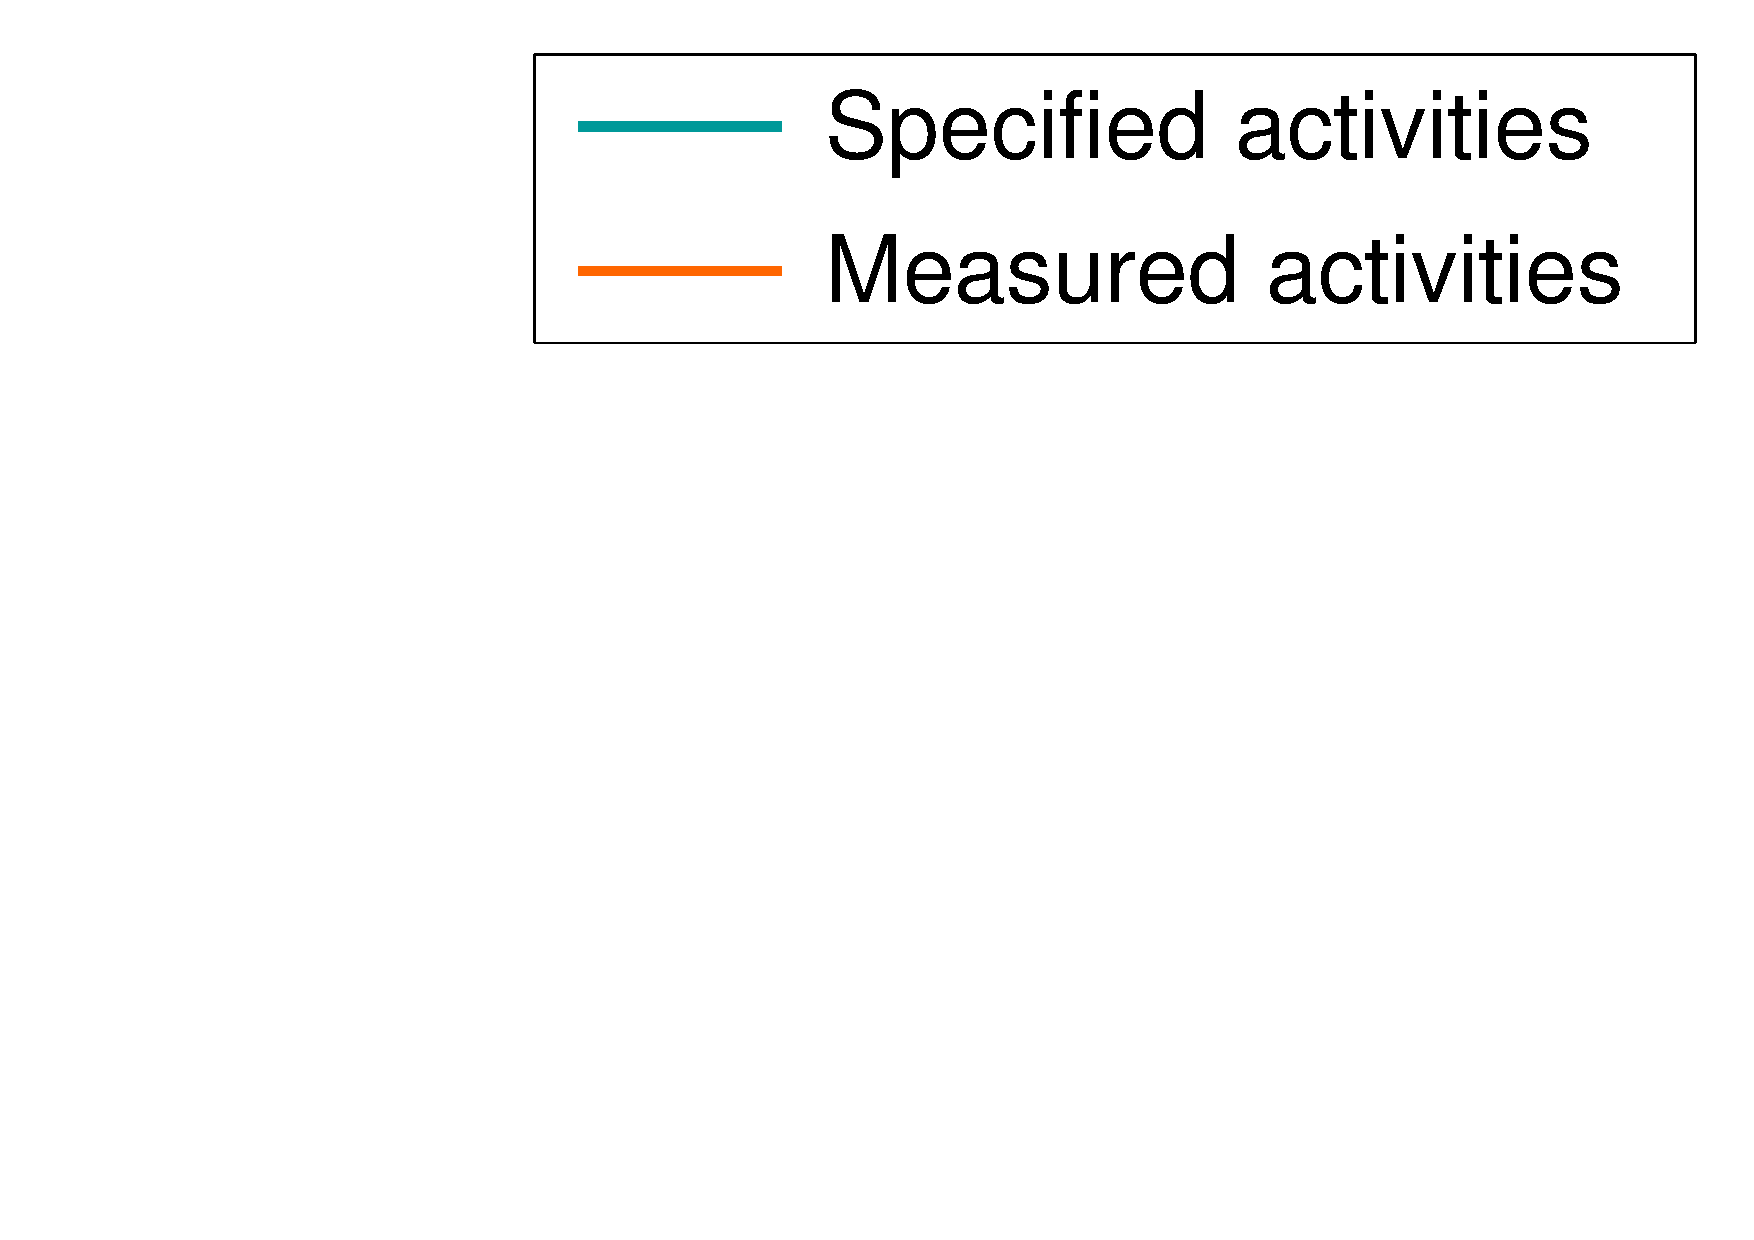
\includegraphics[width=0.5\textwidth]{Sensitivity/fig_sensitivity/legend_cut_Pint.pdf}
  \end{subfigure}
\caption{Total number of expected background in ROI (a),
  evolution of the regions of interest (b),
  $\zeronu$ selection efficiency in ROI (c),
  and limit set on $\Tbeta$ at $90\%$ CL (d),
  as a function of the cut-off applied on distance between vertices, $|~\Delta Z~|$.
  The ROI is optimised for each $|~\Delta Z~|$ cut.
  Results are displayed for two contamination levels: the specified (blue) and the measured (orange) activities (taking into account the upper limit provided for \Bi).
  An exposure of $17.5$~kg.y is considered.
  \label{fig:cont_vertex}}
\end{figure}


\paragraph{}The idea of having implemented these two selections (on the internal probability and on the distance between vertices) comes from a previous NEMO-$3$ analysis on the background rejection.
For the SuperNEMO demonstrator case, the levels of contaminations we are dealing with is remarkably low for most of the topological cut-offs to be worth applying.
However, in practice, applying loose topological selections on the data remains necessary, especially to reject external background events.
The minimal cut-off level to be applied is \Pint~$>~4~\%$ and $|~\Delta~Z~|~<~80$~mm (similarly for $|~\Delta~Y~|$), and can be optimised by taking into account the sources activity.

For future studies, it is useful to give the efficiencies of these loose selections, for the signal and for each background considered (Tab.~\ref{tab:Pint_eff}), as well as the expected number of background in the ROI (Tab.~\ref{tab:Nexp_topo_contamination}).
The selection efficiencies show topological cuts have a huge impact on Radon selection, as they are especially designed to reject non-internal events.
The \Pint\ cut-off is also efficient in rejecting Thallium internal events, because of the existence of a metastable exited state, described earlier.
A special technique to reject efficiently \Tl\ background is also addressed in Chapter~\ref{ch:timediff}.
\begin{table}[h]
  \begin{subtable}[h]{1.\textwidth}
    \centering
    \begin{tabular}{|c|c|c|c|}
      \hline
      Cut-off & First-order cuts (\%) & Internal probability (\%) & Vertex distance (\%) \\
      && \Pint$~>~4\%$ & $|~\Delta~Z~|~<~80$~mm \\
      \hline\hline
      $\zeronu$  & $26.9$ & $25.3$ & $24.7$ \\
      $\twonu$  & $9.15$ & $8.56$ & $8.21$ \\
      \Tl  & $0.106$ & $0.0889$ & $0.0846$ \\
      \Bi  & $0.168$ & $0.151$ & $0.144$ \\
      \Rn  & $0.0177$ & $7.91\times~10^{-3}$ & $5.34\times~10^{-3}$ \\
      \hline
    \end{tabular}
    \captionsetup{justification=justified}
    \caption{Selection efficiencies for the three levels of selection (first-order, \Pint\ and vertex distance), in the full energy range.
      \label{tab:Pint_eff}}
  \end{subtable}
  \vskip\baselineskip
  \begin{subtable}[h]{1.\textwidth}
    \begin{tabular}{|c|c|c|c|c|}
      \hline
      Activity & \multicolumn{2}{c|}{Specified} & \multicolumn{2}{c|}{Measured (w/ \Bi)} \\
      \hline
      Cut-off & \Pint~$>~4~$\% & $|~\Delta~Z~|~<~80$~mm & \Pint~$>~4~$\% & $|~\Delta~Z~|~<~80$~mm  \\
      ROI (MeV) & [$2.7$;$3.15$] & [$2.7$;$3.15$] & [$2.7$;$3.25$] & [$2.7$;$3.3$] \\
      \hline\hline
      $\epsilon_{0\nu}$ & $14.1$\% & $13.9$\% & $14.1$\% & $13.9$\% \\
      \hdashline
      $\twonu$  & $0.392$ & $0.383$ & $0.392$ & $0.383$ \\
      \Tl  & $0.0338$ & $0.0323$ & $1.08$ & $1.09$ \\
      \Bi  & $0.0491$ & $0.0491$ & $1.42$ & $1.42$ \\
      \Rn  & $0.115$ & $0.0782$ & $0.115$ & $0.0782$ \\
      Total & $0.590$ & $0.543$ & $3.01$ & $2.97$ \\
      \hline
    \end{tabular}
    \captionsetup{justification=justified}
    \caption{Selection efficiency of $\zeronu$ events and expected number of backgrounds events in the optimised ROI, for the exposure of the SuperNEMO demonstrator (17.5 kg.y), for successive application of topological selections.
      Specified and measured activities (taking into account the upper limit for \Bi\ contamination) are considered.
      \label{tab:Nexp_topo_contamination}}
  \end{subtable}
  \caption{The selection efficiencies and expected number of background events for the topological selections.}
\end{table}

After the topological cut-off optimisation, the SuperNEMO demonstrator would reach a sensitivity of $\Tbeta~>~5.4\times~10^{24}$~y if specified activities are reached, corresponding to the effective neutrino mass range $\langle\mbb\rangle~<~[0.25-0.48]$~eV.
For the measured activities, supposing \Bi\ activity reaches the measured upper limit, $\Tbeta~>~3.6\times~10^{24}$~y and $\langle\mbb\rangle~<~[0.31-0.59]$~eV.

In the following we review the influence of the $25$~Gauss magnetic field inside the detector on the sensitivity reachable by the SuperNEMO demonstrator, and evaluate the usefulness of the topological cut-offs in that case.

\section{Impact of the magnetic field on the sensitivity}
\label{subsec:field}

The SuperNEMO demonstrator was originally designed with a copper coil, similarly to NEMO-$3$, delivering a magnetic field inside the tracker volume.
This $25$~Gauss magnetic field is high enough to bend the trajectory of the few~MeV electrons and positrons of interest for SuperNEMO, without too strongly preventing them from reaching the calorimeter.
In practice, this magnetic field is mainly used to identify and reject the electron-positron pairs created by high energy $\gamma$’s, themselves emitted after a neutron capture.
However, as explained in sub-section~\ref{subsec:ext_bkg}, we choose to not consider the contribution of this external background for this study's background model.
We therefore focus on evaluating the influence of the presence of the magnetic field on the rejection of natural isotopes disintegrations and on the $\zeronu$ selection efficiency.
%% It is also very useful to better identify the crossing electron events, mostly coming from a 212 Bi contamination on the surface of the calorimeter, as explained in Section 3.2.4.
%% For instance, as shown in Figure 4.1, NEMO-3 observed three events in the [2.8;3.2]MeV region of interest in the one electron one positron channel and two events, induced by high energy $\gamma$’s from neutron capture, with energies higher than 4~MeV.


%% As described in Sec.~\ref{sec:magnetic_field}, the presence of a magnetic field of $25$ G could influence the optical modules performances.
%% In the simulated detector, such effects are not yet implemented, therefore can't be observed in the framework of this analysis.
%% However, possible degradation of the event reconstruction efficiency.



\subsection{Simulations of the magnetic field}

In order to study the influence of the magnetic field on the demonstrator sensitivity to the $\zeronu$ decay, the simulations and reconstructions of signal and backgrounds have been performed in two different conditions.
\begin{itemize}
\item Simulations with a uniform $25$ Gauss magnetic field (following recommendations \cite{CalvezThesis}).
  Results about the final sensitivity achieved in this condition have already been presented earlier in this chapter.
  The possible variations of the field intensity, mainly due to the calorimeter magnetic shields, are not taken into account for these simulations.
  This will be discussed in sub-section~\ref{subsec:mapped_field}.
\item Simulations where the magnetic field is turned off.
%\item simulations with a $25$ Gauss \emph{mapped} magnetic field, taking into account more realistic variations of the magnetic field inside the detector~\cite{docdb:map_magnetic_field2015}.
\end{itemize}
Each magnetic field condition has the same number of simulated events, as summed up in Tab.~\ref{tab:sensitivity_simulations}.

Depending on the case under consideration, the charged particles do not have the same trajectory curvature.
In the first uniform on-field case, they are bended.
The track fit algorithm then performs two distinct trajectory fittings: one with a helix and one with a line.
The most accurate fit is chosen and provides information on the charge of the detected particle.
In the second off-field case, the fitting algorithm is modified to fit only linear trajectories.
%Finally, the best tracking option (line or helix) for the third mapped on-field case is discussed in the next section.

\subsection{Impact of the magnetic field on signal and background selections}
\label{subsec:impact_field}
%%%

Among first-order event selection criteria considered in Sec.~\ref{sec:sensitivity_ev_selection}, the one on the trajectory curvature is of primary importance with regard to the influence of the magnetic field on the final sensitivity.
Indeed, when the magnetic field is switched on, a particle is identified as an electron when the trajectory fitting results in a negative curvature.
When the magnetic field is switched off, the trajectory of the charged particles takes place in a straight line\footnote{In saying this, we do not take into account possible deviations in the trajectory of the particles, due in particular to multiple scattering in the tracker.}.
This last selection criterion on the track curvature is then no longer applied.

Consequently, the number of identified $2e$ topologies selected by the first-order cuts is increased for the off-field case because the event selections are less strict.
To illustrate this effect, we give in Tab.~\ref{tab:eff_on_off} the selection efficiencies of signal and background in the total energy range [$0$;$4$]~MeV, for the two cases of magnetic field.
The $\zeronu$ efficiency increases, as well as the one of backgrounds.
In particular, the Radon efficiency increases very significantly.
Indeed, in some cases, the two electrons resulting from the decay of Bismuth on the tracker wires can be emitted back to back.
One of the two electrons can subsequently pass through the source in the direction of the opposite calorimeter.
%%%%In that case there is a kink between track going to sc. and part of track going to source
%%%%Therefore the ability to reconstruct an helix is less probable
When this decay takes place close to the source, it is arduous to reconstruct a helix in the presence of a magnetic field, and this type of event is easily rejected.
Whereas without a field there is no selection of curvature so these events are more likely to be selected.
\begin{table}[h!]
  \centering
  \begin{tabular}{|c|c|c|}
    \hline
    Field & On & Off \\
    \hline\hline
    $\zeronu$  & $26.9$ & $31.4$ \\
    $\twonu$  & $9.16$ & $10.6$ \\
    \Tl  & $0.106$ & $0.169$ \\
    \Bi  & $0.168$ & $0.252$ \\
    \Rn  & $0.0177$ & $0.0924$ \\
    \hline
  \end{tabular}
  \caption{Selection efficiencies (\%) in the full energy range [$0$;$4$]~MeV, for on and off-field cases.
    First-order cut-offs have been applied.
    \label{tab:eff_on_off}}
\end{table}

%% The field being turned-off, electrons and positrons are no more discriminated, enhancing the number of $2e$ topologies selected.
We compare the variations of selection efficiencies in the ROI these in Tab.~\ref{tab:eff_field} for the two field cases.
The selection efficiencies of $\beta\beta$ decays are disadvantaged by the lower bound of the ROI for the off-field case.
The slight variation of the ROI upper bound have a measurable impact on the expected number of \Tl\ events, as this background has a contribution at high energies.
The increase of \Rn\ events, despite the ROI lower bound variation, is directly explained by the phenomenon, described above, of selecting $2e$ events issued back to back close to the source.
These observations result in a decrease in sensitivity when the field is switched off, giving
%%%%the red. in 0nu eff and decrease of bkg leads globally to decrease sens.
\begin{equation}
\Tbeta > 4.8\times 10^{24}\,\text{y}\qquad (90\% \text{CL})\, (\text{off-field}).
\end{equation}
\begin{table}[h!]
  \centering
  \begin{tabular}{|c|c|c|}
    \hline
    Field & On & Off \\
    & [$2.7$;$3.15$]~MeV & [$2.75$;$3.2$]~MeV \\
    \hline\hline
    $\epsilon_{0\nu}$ & $14.7$\% & $12.4$\% \\
    \hdashline
    $\twonu$  & $0.418$ & $0.0353$ \\
    \Tl  & $0.0475$ & $0.0600$ \\
    \Bi  & $0.0546$ & $0.0452$ \\
    \Rn  & $0.292$ & $0.553$ \\
    Total & $0.812$ & $0.693$ \\
    \hline
  \end{tabular}
  \caption{Selection efficiency of $\zeronu$ events and expected number of backgrounds events in the optimised ROI, for the exposure of the SuperNEMO demonstrator (17.5 kg.y).
    Specified activities are considered.
    The two on- and off-field cases are compared.
    First-order cut-offs have been applied.
    \label{tab:eff_field}}
\end{table}

As concluded in Sec.~\ref{sec:demonstrator_sensitivity}, topological selections are especially efficient in rejecting the Radon background.
Therefore, the application of these additional cut-offs, for the off-field case, could be interesting, in order to increase the sensitivity.
Following the work presented in the previous section, we optimise these selections for the particular off-field case, both for the specified and measured contamination levels\footnote{As done in sub-section~\ref{subsec:opti_ev_selection}, for the Bismuth measured contamination, we consider here the upper limit where $\mathcal{A}^{\text{Bi}}=290~\mu$Bq/kg.}.
Fig.~\ref{fig:sensitivity_B} summarises the results obtained in sensitivity before and after application of these topological cut-offs.
The left part of the panel gives information on the evolution of sensitivity, when only the first-order cut-offs are applied.
We come back to the conclusions given above: when the magnetic field is switched-off, we lose sensitivity, regardless of the level of contamination considered.
On the right side of the figure, we present the results when the topological cuts are applied.
For the on-field case, the addition of these selections have almost no effect on the sensitivity, as concluded in sub-section~\ref{subsec:opti_ev_selection}.
However, as predicted, we are beginning to see the usefulness of these selections in the off-field case, as a higher number of \Tl\ and \Rn\ events passed the first-order selections.
For instance, for the specification case, $\Tbeta$ goes from $4.8\times 10^{24}\,\text{y}$ to $6.1\times 10^{24}\,\text{y}$, an improvement of~$\sim~30\%$.
\begin{figure}[h!]
  \centering
  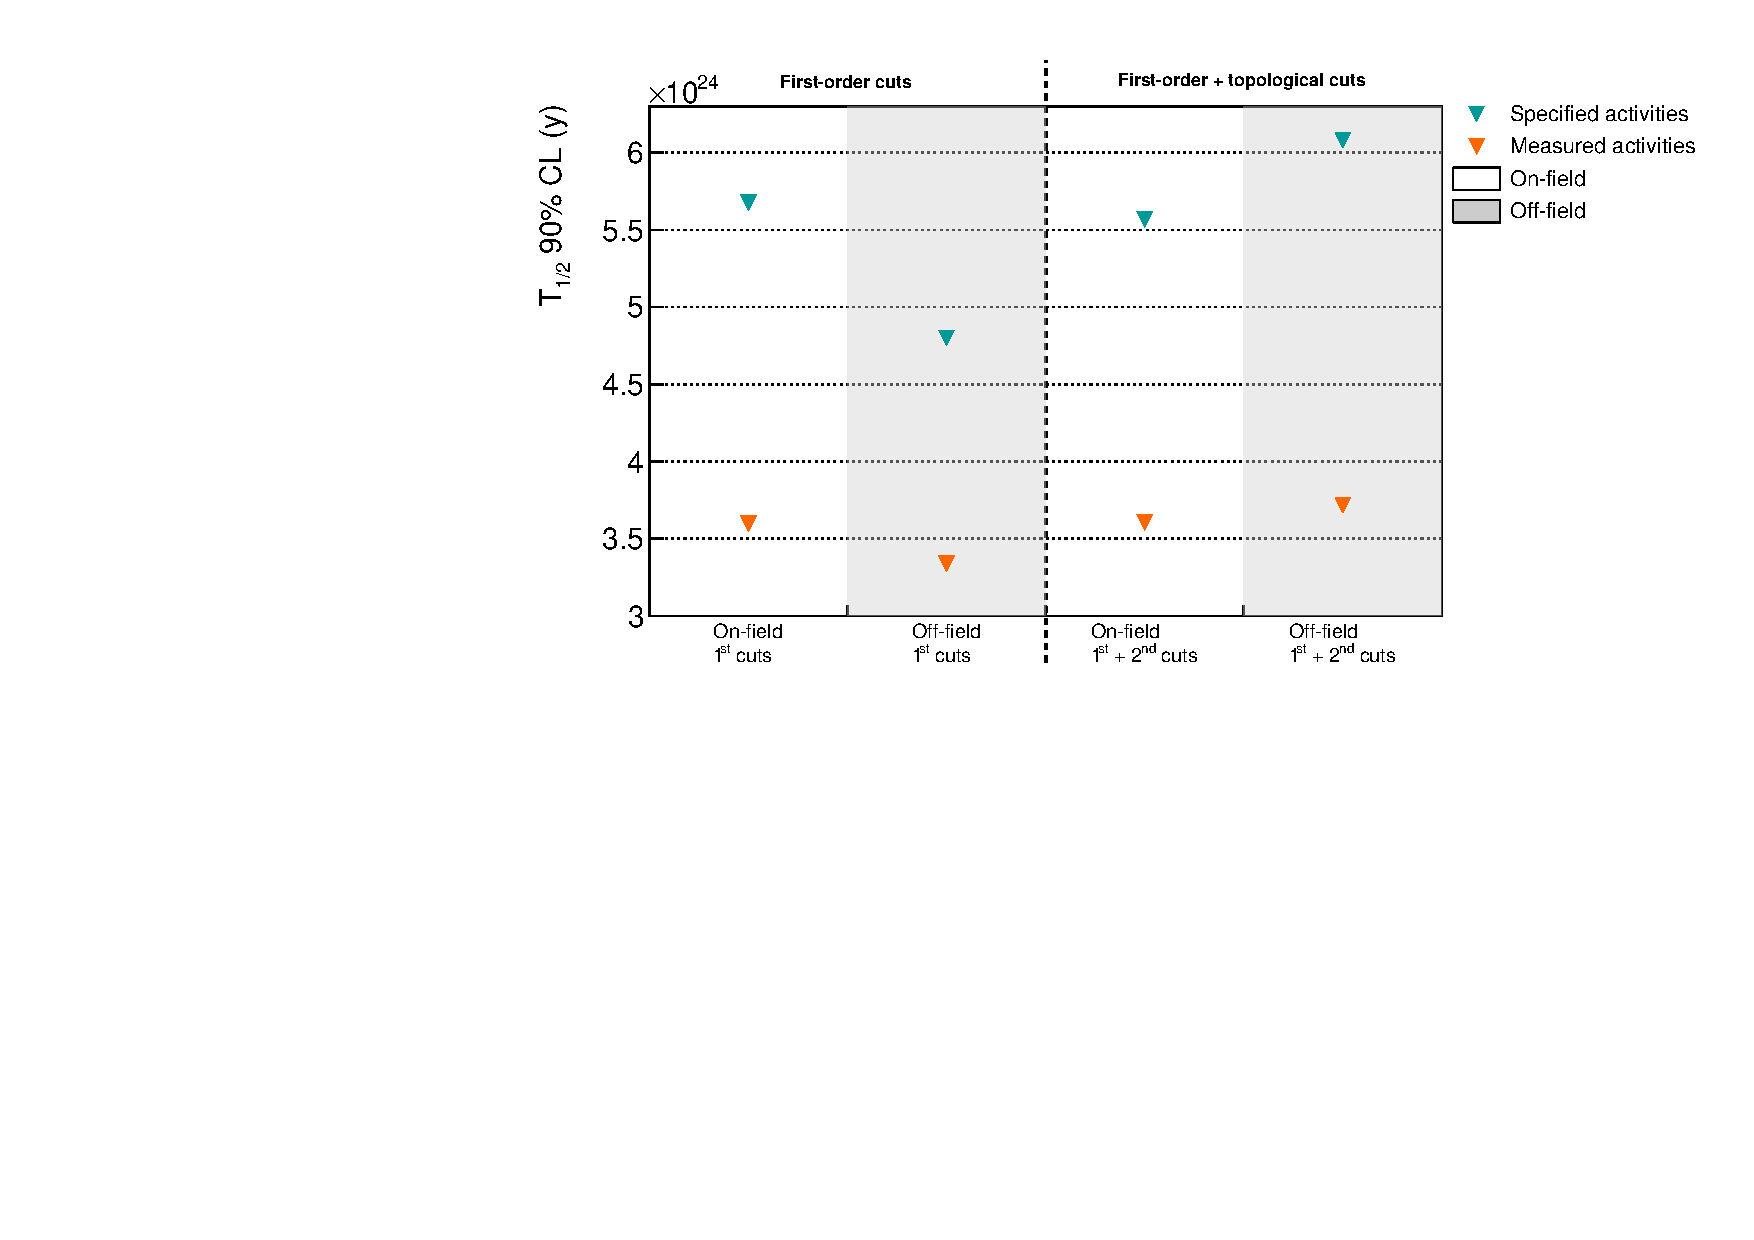
\includegraphics[width=1.\textwidth]{Sensitivity/fig_sensitivity/contamination_Se_w_woB.pdf}
  \caption{$\Tbeta$ ($90$\% CL) considering various conditions: on- and off-field (white and grey stripes), first-order and addition of topological cut-offs (left/right parts of the panel), specified and measured activities (blue and orange triangle markers).
    The measured activities are $\mathcal{A}^{\text{Tl}}=54~\mu$Bq/kg, $\mathcal{A}^{\text{Bi}}=290~\mu$Bq/kg and $\mathcal{A}^{\text{Rn}} = 0.15$~mBq/m$^{3}$.
    \label{fig:sensitivity_B}}
\end{figure}

In Tab.~\ref{tab:Nexp_noField} are presented the expected number of background events in the ROI for the off-field condition, before and after application of topological cut-offs, for the specified and measured activities (taking into account the upper limit for the \Bi\ contamination).
This selection allows to reject mainly \Rn\ background.
\begin{table}[h!]
  \centering
  \begin{tabular}{|c|c|c|c|c|}
    \hline
    Activity & \multicolumn{2}{c|}{Specified} & \multicolumn{2}{c|}{Measured (w/ \Bi)} \\
    \hline
    Cut-off & First-order & Topological & First-order & Topological  \\
    ROI (MeV) & [$2.75$;$3.2$] & [$2.7$;$3.2$] & [$2.65$;$2.9$] & [$2.7$;$2.9$] \\
    \hline\hline
    $\epsilon_{0\nu}$ & $12.4$\% & $15.7$\% & $19.1$\% & $14.8$\% \\
    \hdashline
    $\twonu$  & $0.0353$ & $0.453$ & $1.56$ & $0.440$ \\
    \Tl  & $0.0600$ & $0.0506$ & $1.01$ & $0.613$ \\
    \Bi  & $0.0452$ & $0.0706$ & $2.94$ & $1.84$ \\
    \Rn  & $0.553$ & $0.0894$ & $1.42$ & $0.0689$ \\
    Total & $0.693$ & $0.664$ & $6.93$ & $2.96$ \\
    \hline
  \end{tabular}
  \caption{Selection efficiency of $\zeronu$ events and expected number of backgrounds events in the optimised ROI, for the exposure of the SuperNEMO demonstrator (17.5 kg.y), with off-field condition.
    Specified and measured (with \Bi) activities are considered.
    Topological cut-offs are optimised: \Pint$>4$\% and $|\Delta Z|<80$mm (specified activities),  \Pint$>5$\% and $|\Delta Z|<80$mm (measured activities)
    \label{tab:Nexp_noField}}
\end{table}

Finally, even if the absence of the magnetic field has the effect of reducing the sensitivity to the $\zeronu$ decay, topological cuts allow this effect to be compensated for, making it possible to reach higher values of $\Tbeta$.

%% \begin{itemize}
%% \item pour la variation de la ROI dans la figure comparative des différents level en contaminations : la ROI bouge pour les cas measured. C'est étonnant à premièer vue car ça ne paraît pas optimal et ça rajoute du Bi. Mais en fait si on regarde  les biplots de sensibilité, on a des fluctuations. Mais ce ne sont pas de grosses fluctuations, ce qui est aussi rassurant car ça veut dire qu'on n'est pas trop sensible aux variations de Emin/Emax (même si j'ai dit qu'on y était pas mal sensible -> à regarder)
%% \end{itemize}

\subsection{Influence of the magnetic field on optical modules and reconstruction efficiency}

In the previous sub-section, a comparative study has been led to evaluate the influence of the presence of a magnetic field on the event selection, and thus on the final sensitivity.
However, as things stand now, some features of the demonstrator are not yet implemented in the simulation software, and could have a great impact on the results presented above.
In particular, studies have been led by the collaboration to evaluate the influence a $25$~Gauss magnetic field on the optical modules, as well as on the event reconstruction~\cite{CalvezThesis,internal:magnetic_field}.

SuperNEMO PMTs are protected from the external magnetic field by individual iron shields.
Unfortunately, the latter do not perfectly protect the PMTs, and a residual magnetic field is measured inside the shieldings, leading to losses in charge collected by PMTs close to $8\%$.
This study also revealed the energy resolution would be worsened with a relative decrease of $3\%$ of the initial value of $8\%$ at $1$~MeV.
Moreover, the PMTs shieldings could themselves severely impact the shape of the field lines, as well as its intensity.
In fact, with a $25$ Gauss magnetic field generated by the copper coil, the magnetic shields are responsible for the field strength decreasing, and barely $10$ G is expected near the source foils.
Worse, the magnetic field strength decreases very quickly as we get closer to the calorimeter walls, where nearly $0~$G could be expected.
The reconstruction efficiency could therefore be greatly impacted:
the magnetic field intensity varying from the source foils to the calorimeter wall, electrons trajectory curvatures are not constant, and the track-fitting algorithm is less performing.
An incorrect description of the distribution of the magnetic field would more strongly impact low-energy electrons.

In the light of these conclusions, it could be interesting to study the evolution of the sensitivity, considering field simulations with more realistic variations inside the detector.

%% Despite the fact that magnetic shields were designed and installed to protect the PMTs, this field can have a great impact on the calorimeter detection efficiency, and thus could degrade the detector's sensitivity to the $\zeronu$ decay.

\subsection{Simulations with a non-uniform magnetic field}
\label{subsec:mapped_field}

Simulations with a $25$~Gauss \emph{mapped} magnetic field have been performed, taking into account more realistic variations of the field inside the detector~\cite{docdb:map_magnetic_field2015}.
In this condition, the fitting algorithm follows the same steps as for on-field: a helix and linear fit are performed for each simulated event, and the most accurate is selected.
Unfortunately, Radon isotope decays could not be simulated with this magnetic field configuration.
Indeed, as it is present in the entire wire chamber, simulations would have required too many additional storing resources.
Thus, strong conclusions on the sensitivity can't be given.
However, it is possible to assess the selection efficiencies of the different processes, and then get an idea of the influence of realistic variations of the field on the final results.
%% Fig.~\ref{} displays
%% \begin{figure}[h!]
%%   \centering
%%   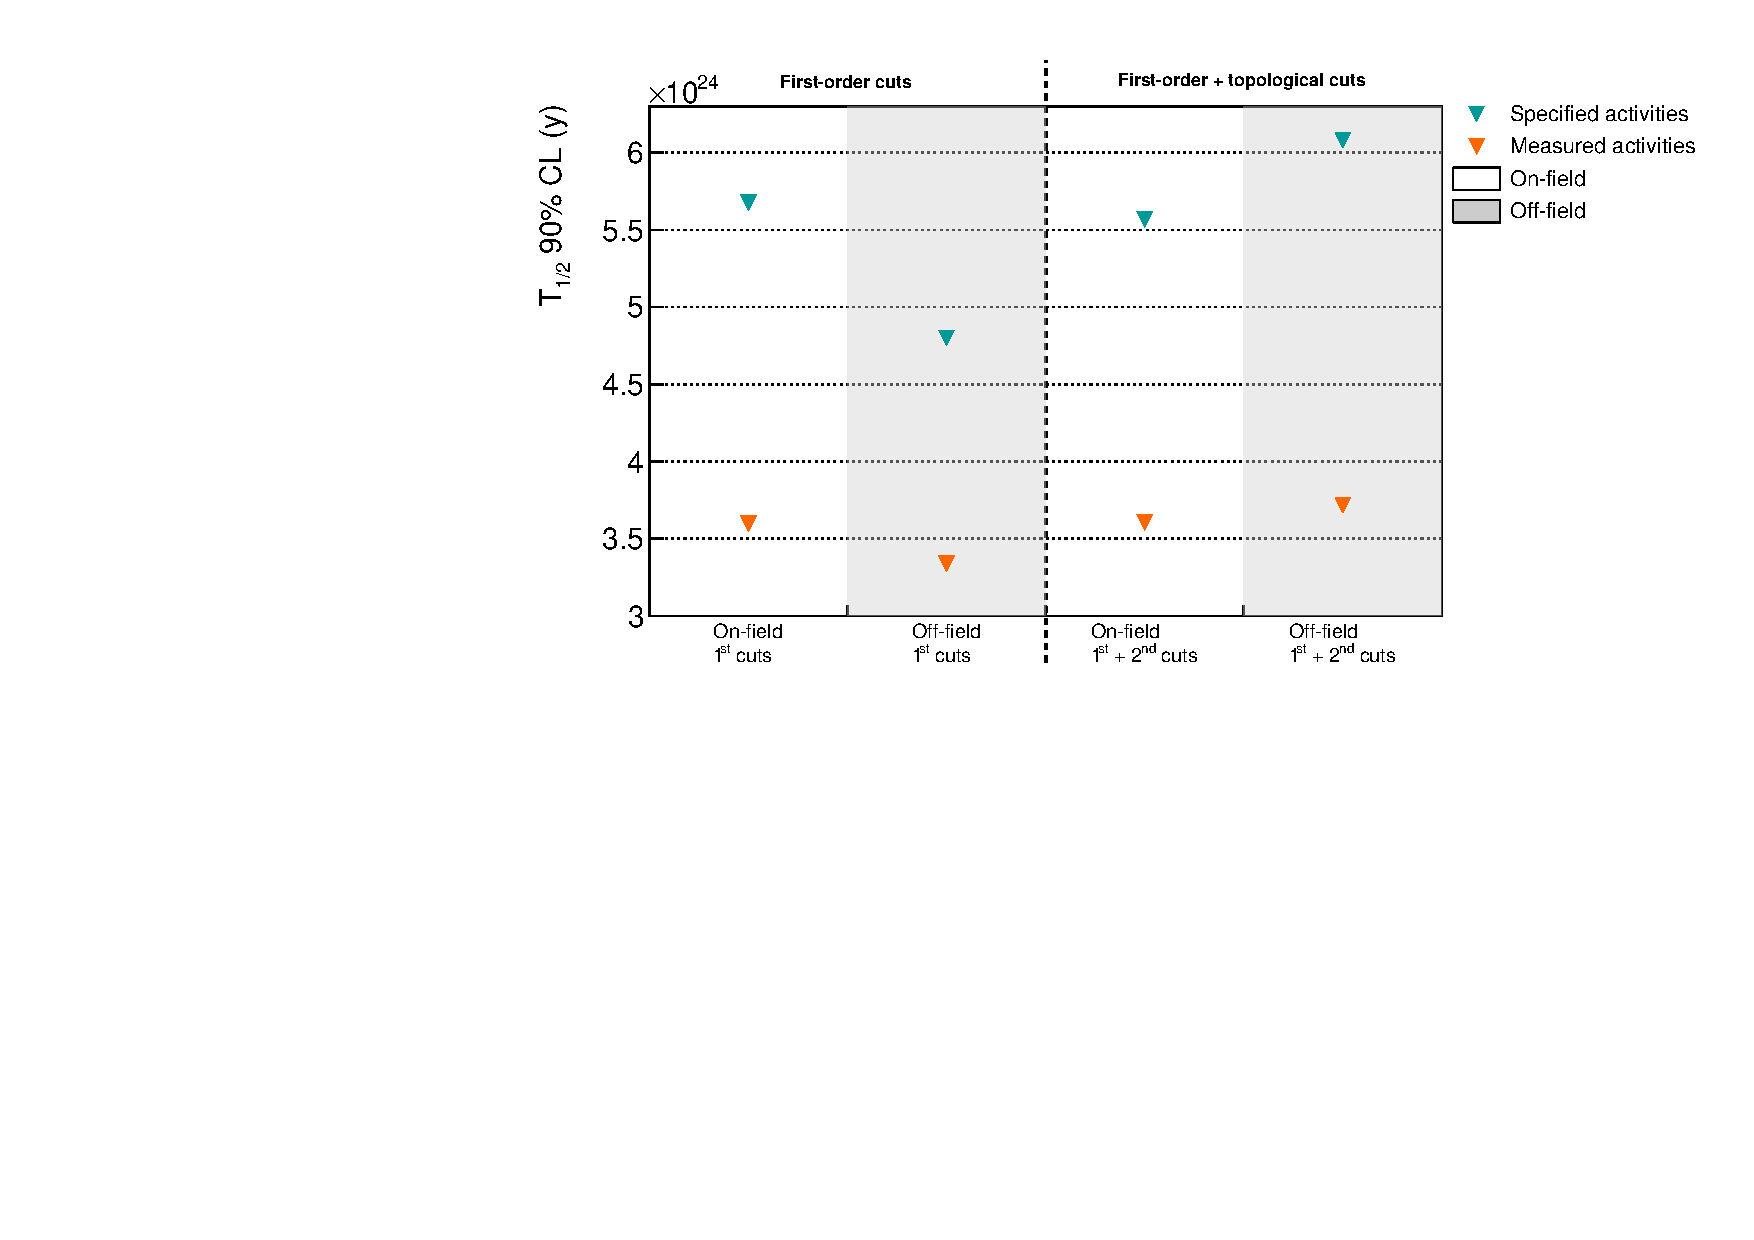
\includegraphics[width=1.1\textwidth]{Sensitivity/fig_sensitivity/contamination_Se_w_woB.pdf}
%%   \caption{Best limit set on $\zeronu$ half-life (top pad), and the corresponding ROI (bottom pad), as a function of the contamination level considered, for both on-field and off-field cases.
%%     \label{fig:}}
%% \end{figure}

Tab.~\ref{tab:mapped_eff} compares the selection efficiencies, for the three field cases (uniform on-field, mapped field and off-field), in the total energy range [$0$;$4$]~MeV.
The mapped field case has lower selection efficiencies, compared with uniform field simulations.
As announced in the previous sub-section, the magnetic shields distort the field intensity across the detector.
Therefore, the fitting algorithm is less efficient in identifying particles with a negative curvature inside the tracker, hence the number of selected $2e$ topologies is decreased.
\begin{table}[h!]
  \centering
  \begin{tabular}{|c|c|c|c|}
    \hline
    Field & On & Off & Mapped  \\
    \Pint & \Pint$>4$\% & \Pint$>1$\% & \Pint$>4$\% \\
    \hline\hline
    $\zeronu$ & $24.7$ & $29.3$ & $19.1$ \\
    $\twonu$ & $8.21$ & $9.93$ & $6.39$ \\
    \Tl & $0.0846$ & $0.140$ & $0.0774$ \\
    \Bi & $0.144$ & $0.211$ & $0.125$ \\
    \hline
  \end{tabular}
  \caption{Signal and background selection efficiencies (\%) for on-field, off-field and mapped-field cases, in the energy range [$0$;$4$]~MeV.
    The first-order and optimised topological cut-offs have been applied.
    Especially, for all field conditions, $|\Delta~Z|<80$~mm.
  \label{tab:mapped_eff}}
\end{table}

Tab.~\ref{tab:eff_mapped_ROI} presents the expected number of background events in the energy range [$2.7$;$3.2$]~MeV, for simulations using the realistic mapped field.
As expected, the $\zeronu$ selection efficiency is drastically decreased compared with the on-field case, as well as the expected number of background events.
As explained above, the selection on track curvature is still applied in this case, and the non-uniform magnetic field causes deviations in the particles trajectory, which are therefore more difficult to identify as electrons.
Even if Radon simulation with such field conditions are unavailable, it is interesting to provide an order of magnitude of the $\Tbeta$ limit set with these realistic variations of the field.
To do so, we extrapolate the expected number of Radon events in the [$2.7$;$3.2$]~MeV energy range, from the \Bi\ one.
Indeed, we postulate the ratio between these two numbers remains constant, and the on-field simulations give $N_{\text{Bi}}/N_{\text{Rn}}\sim5$.
Taking this into consideration, a limit of $\Tbeta~>~4\times~10^{24}$~y ($90$~\% CL) would be reached with the demonstrator, a $\sim 30$~\% decrease compared with the non-realistic uniform case.

This approximation should be examined with caution, however, as magnetic field conditions can greatly influence the selection of Radon and Bismuth events.
To be specific, we have seen in Sec.~\ref{subsec:impact_field} that between off-field and on-field conditions, the Radon and Bismuth efficiencies varied differently.
So, to ensure that our approximation is valid, a more proper study would have to be made.
In particular, it would be necessary to study how events where the two electrons are emitted back to back from a wire of the tracker when the field is no longer uniform are treated.
\begin{table}[h!]
  \centering
  \begin{tabular}{|c|c|}
    \hline
     & Mapped field  \\
    \hline\hline
    $\epsilon_{0\nu}$ & $10.4$\%  \\
    \hdashline
    $\twonu$  & $0.245$  \\
    \Tl  & $0.0279$  \\
    \Bi  & $0.0535$  \\
    Total & $0.326$ \\
    \hline
  \end{tabular}
  \caption{Selection efficiency of $\zeronu$ events and expected number of backgrounds events in the [$2.7$;$3.2$]~MeV optimised ROI, for the exposure of the SuperNEMO demonstrator (17.5 kg.y), for mapped field simulations.
    The specified background activities are considered.
    First-order and optimised topological cuts have been applied (\Pint$>4$\% and $|\Delta~Z|<80$~mm).
    \label{tab:eff_mapped_ROI}}
\end{table}

\section{Searching for the \Nd\ $\zeronu$ decay}
\label{sec:Nd}

This study was conducted jointly with the PhD student Axel Pin, from CENBG~\cite{AxelThesis}.
Although we mainly developed together the whole analysis, I presented in detail in the previous sections the results regarding the influence of the magnetic field.
Meanwhile, Axel Pin focuses on the possibility of changing the \Se\ material by other $\beta\beta$ isotopes.
Indeed, on the model of the NEMO-$3$ detector, which housed, among others, $6.914$~kg of \Mo\ and $0.932$~kg of \Se, the SuperNEMO detector possesses the technical possibility of exchanging the source material and study several $\beta\beta$ isotopes.
Notably, in the case SuperNEMO demonstrates the feasibility of a large-scale tracko-calo experiment, it would be natural to  evaluate the sensitivity of SuperNEMO to the $\zeronu$ decay of other isotopes than \Se.

\subsection{Searching for the $\zeronu$ of other isotopes}

One of the distinctive features of NEMO detectors is the gaseous detector, designed to track charged particles.
Unluckily, this advantage is also a great inconvenience when it comes to Radon contamination.
Indeed, Radon enters by diffusion or emanates from the detector materials.
It is then interesting to consider $\beta\beta$ candidates with an energy transition value above the $Q_{\beta}=3.27$~MeV of \Bi, a \Rn\ daughter.
Another useful criterion is the natural isotopic abundance: typically, considering only isotopic abundances greater than 2\% is a reliable basis when selecting potential $\beta\beta$ emitters.
Two nuclei satisfy these two criteria: $^{96}$Zr and \Nd\ (with respective $\Qbb$ values of $3.35$ and $3.36$~MeV, and respective isotopic abundances of $2.8$ and $5.6$~\%~\cite{art:atomic_mass}).
%% Given the availability of \Mo, much effort has been focused by the NEMO-$3$ collaboration on this isotope (it had already been studied by the NEMO-$2$ prototype~\cite{art:NEMO2}).
As the \Nd\ isotope has the highest $\Qbb$ value, the current section focuses on evaluating the SuperNEMO sensitivity to the $\zeronu$ decay of this isotope, supposing we have several kg at our disposal.
Moreover, the \Nd\ has a more favourable phase space than the \Se, on which the half-life limit directly depends.

\subsection{Sensitivity to the $\zeronu$ of \Nd}

Until recently, \Nd\ was not enrichable in large quantities.
Recent developments have resulted in the production of several grams, making this $\beta\beta$ isotope interesting for the search for $\zeronu$.
Thanks to that, NEMO-$3$ had available $36.6$~g of \Nd\ which were recovered by the collaboration, for a possible reuse for SuperNEMO.
The best limit for the search for neutrinoless double $\beta$ decay of \Nd\ was reached by the NEMO-$3$ detector with $5.25$~years of data acquisition.
The detector achieved $\Tbeta~>~2.0\times~10^{23}$~y~($90$~\%~CL), corresponding to a range on the effective neutrino mass of $\langle\mbb\rangle~<~[1.6-5.3]$~eV.
The collaboration also measured the $\twonu$ half-life, with $\Ttwonu~=~$[$9.34~\pm~0.22$~(stat.)~$\pm~^{0.62}_{0.60}$~(syst.)]$\times~10^{18}$~y~\cite{art:NEMO3_Nd}.

We wish to determine the limit on the $\zeronu$ of the \Nd\ that could be reached with the SuperNEMO demonstrator, with an exposure of $17.5$~kg.y.
We lead this study considering the activities specified for the \Se\ sources are reached.
We use simulations with the $25$~Gauss uniform magnetic field.
Fig.~\ref{fig:energy_Nd} depicts the normalised energy distributions for the $2e$ topologies selected after application of first-order and topological selections.

%%, considering that the impact of the $\beta\beta$ isotope proton number on electrons crossing the foils in negligible.

Signal and background selection efficiencies for \Nd\ sources, in the total energy range, are given in Tab.~\ref{tab:energy_spect_Nd}.
The selection efficiencies of backgrounds are lower for \Nd\ sources than for \Se\ sources.
In both cases, for the total energy range the background contribution is dominated by the $\twonu$ decay.
This is caused by the more elevated number of protons in the \Nd\ nucleus which induces a stronger Coulombian effect.
Indeed, the more the $\beta\beta$ emitter has a high atomic number $Z$, the more the electrons emitted from inside the source (or passing through it) are likely to interact electromagnetically with it.
Despite this, for reasons of limited storage resources, we choose to consider this effect to be negligible for events outside the source, such as \Bi\ disintegrations (from \Rn) from the tracker wires, and we choose to use the Radon simulations already generated for the \Se\ sources study.
Clearly, future studies would rather use a new set of simulations for \Rn\ events and evaluate its influence on the sensitivity.
\begin{figure}[h!]
  \centering
  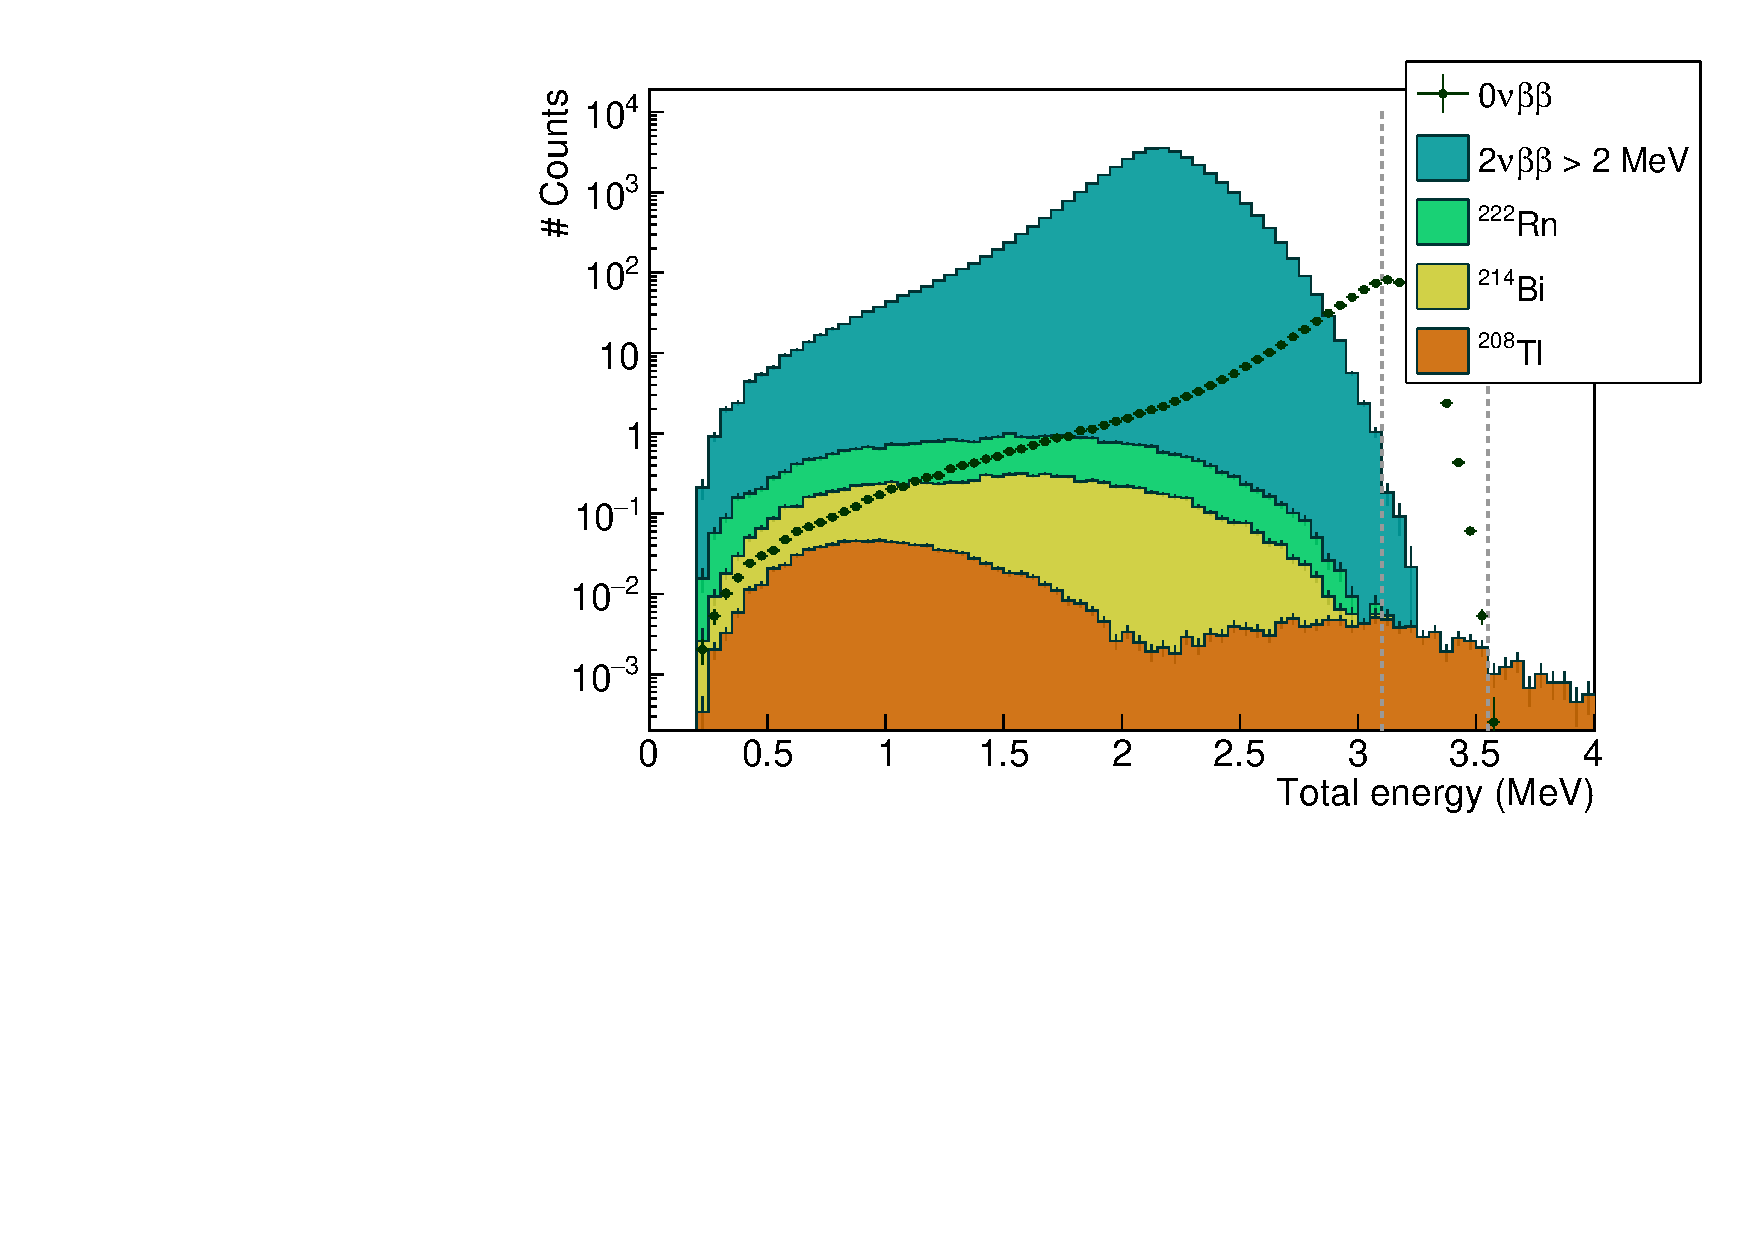
\includegraphics[width=0.8\textwidth]{Sensitivity/fig_sensitivity/energy_spectrum_with_B_150Nd.pdf}
  \caption{Total energy spectra for the $\zeronu$ signal and main backgrounds, for \Nd\ sources and for a $17.5$~kg.y exposure.
    The $\twonu$ spectrum is normalised to $\Ttwonu~=~9.34\times~10^{18}$~y, and \Tl, \Bi\ and \Rn\ backgrounds are normalised to the nominal activities.
    The amplitude of the $\zeronu$ is arbitrarily set at the limit obtained with NEMO-$3$ $\Tbeta~=~2.0\times~10^{23}$~y.
    First-order and optimised topological cuts have been applied.
    The ROI of [$3.1$;$3.55$]~MeV is depicted by to vertical dashed lines.
    \label{fig:energy_Nd}}
\end{figure}
\begin{table}[h!]
  \centering
  \begin{tabular}{|c|c|c|}
    \hline
    Isotope & \Se\ & \Nd\ \\
    \hline\hline
    $\zeronu$  & $25.8$ & $25.5$ \\
    $\twonu$  & $8.21$ & $8.11$ \\
    \Tl  & $0.0846$ & $0.0749$ \\
    \Bi  & $0.144$ & $0.138$ \\
    \Rn  & $5.34\times 10^{-3}$ & $5.34\times 10^{-3}$ \\
    \hline
  \end{tabular}
  \caption{Selection efficiencies in the full energy range [$0$;$4$]~MeV, for \Se\ and \Nd\ sources.
    First-order and optimised topological cuts have been applied.
    \label{tab:energy_spect_Nd}}
\end{table}

In Tab.~\ref{tab:Nexp_Nd_ROI} we give the expected number of background events in the optimised ROI [$3.1$;$3.55$]~MeV.
The selection efficiency of the $\zeronu$ decay in this energy range is also given.
Although the $\twonu$ half-life of the \Nd\ is lower than that of the \Se\ by a factor $\sim~10$, the number of $\twonu$ events in the ROI remains low.
Indeed, thanks to the Coulombian effects described above, this process has a limited contribution at high energy.
The high energy of transition $\Qbb~=~3.36$~MeV of \Nd\ implies that the contributions of \Bi\ and \Rn\ are very small, or even zero, because the ROI is optimised in a high energy range.
The $\twonu$ and \Tl\ events are therefore the major contributors to the background.
Consequently, if the choice of changing the source material with \Nd\ isotope was made, it would be conceivable to release the specifications on \Bi\ and \Rn\ backgrounds.
\begin{table}[h!]
  \centering
  \begin{tabular}{|c|c|c|}
    \hline
    Isotope & Selenium & Neodymium \\
    ROI & [$2.7$;$3.15$]~MeV & [$3.1$;$3.55$]~MeV \\
    \hline\hline
    $\epsilon_{0\nu}$ & $14.4$\% & $10.3$\% \\
    \hdashline
    $\twonu$  & $0.39$ & $0.28$ \\
    \Tl  & $0.044$ & $0.029$ \\
    \Bi  & $0.053$ & $5.6\times 10^{-4}$ \\
    \Rn  & $0.20$ & $0.0$ \\
    Total & $0.687$ & $0.309$ \\
    \hline
  \end{tabular}
  \caption{Selection efficiency of $\zeronu$ events and expected number of backgrounds events in the optimised ROI, for the exposure of the SuperNEMO demonstrator (17.5 kg.y), for \Se\ and \Nd\ sources.
    The specified background activities are considered.
    First-order and optimised topological cuts have been applied.
    \label{tab:Nexp_Nd_ROI}}
\end{table}

The SuperNEMO demonstrator, with $7$~kg of \Nd\ and $2.5$~years of data acquisition, would achieve a $\Tbeta~>~2.2\times~10^{24}$~y sensitivity, one order of magnitude higher than the best limit ever reached.
The corresponding limit on the effective neutrino mass is $\langle\mbb\rangle~=~[0.15-0.50]$~eV.
This is a better result than for \Se\ sources, as the \Nd\ has a more favourable phase space factor.


\section{The final detector sensitivity}

The ultimate goal of the SuperNEMO demonstrator is to show that the NEMO technology is scalable to probe unprecedented half-life on the $\zeronu$ decay.
The final detector would consist in building $20$ modules similar to the demonstrator.
In this context, we estimate the final detector sensitivity to the $\zeronu$ decay.

We suppose the specified activities of $\mathcal{A}^{\text{Tl}} = 2~\mu$Bq/kg, $\mathcal{A}^{\text{Bi}} = 10~\mu$Bq/kg and $\mathcal{A}^{\text{Rn}} = 0.15$ mBq/m$^{3}$ are reached.
The simulations with an uniform magnetic field are used.

Tab.~\ref{tab:Nexp_HN} shows the number of expected events in the optimised ROI for first-order and topological cut-offs.
The total expected number of background events is high enough for the optimised cut-offs to be worth it, with \Pint\ $>~4~\%$ and $|\Delta~Z|~<80$~mm (similarly for $|\Delta~Y|$).
They allow primarily to reduce the Radon background by a factor $3$.
Due to the optimisation of the ROI, especially to the raising of the upper bound, the \Tl\ background is a little increased, without important consequences, as the $\twonu$ and \Rn\ dominate the total number of background in this energy range.
\begin{table}[h!]
  \centering
  \begin{tabular}{|c|c|c|}
    \hline
    Cut & First-order & Topological  \\
    ROI & [$2.75$;$2.95$] MeV & [$2.75$;$3.1$] MeV \\
    \hline\hline
    $\epsilon_{0\nu}$ & $11.3$\% & $10.7$\%  \\
    \hdashline
    $\twonu$  & $3.48$ & $3.36$  \\
    \Tl  & $0.728$ & $0.756$  \\
    \Bi  & $0.945$ & $0.835$  \\
    \Rn  & $6.93$ & $2.16$  \\
    Total & $12.1$ & $7.11$ \\
    \hline
  \end{tabular}
  \caption{Selection efficiency of $\zeronu$ events and expected number of backgrounds events in the optimised ROI, for the exposure of the SuperNEMO final detector ($500$~kg.y).
    The specified background activities are considered.
    The topological selections have been optimised: \Pint$>4$\% and $|\Delta~Z|<80$~mm.
    \label{tab:Nexp_HN}}
\end{table}

With an exposure of $500$~kg.y, the SuperNEMO final detector would reach a sensitivity of $\Tbeta~>~5.4\times~10^{25}$~y, with \Se\ sources, corresponding to $\langle\mbb\rangle~=~[0.079-0.15]$~eV.
By comparison, with the same exposure and background specifications but with \Nd\ sources, the final detector would achieve a sensitivity of $\Tbeta~>~2.2\times~10^{25}$~y, in the [$3.1$;$3.75$]~MeV ROI, corresponding to $\langle\mbb\rangle~=~[0.046-0.15]$~eV.


\section{Conclusion}

Latest measurements of source activities by BiPo-$3$ show that the specified background level for Thallium isotope is not reached, although it is improved on average by a factor $2$, compared to NEMO-$3$.
An upper limit is given for the internal Bismuth isotope activity.
In addition, not all sources were measured and a precise measurement is expected to be provided by the SuperNEMO demontrator when data acquisition will begin.
C-sections measurements with a concentration line showed the Radon targeted activity can be achieved for the demonstrator, with an gas flow rate of $2$~m$^{3}$/h inside the chamber.
Topological selections, designed to reject non-internal and non-simultaneous $2e$ events, have been optimised, and allowed to reduce the Radon background by a factor $3$ for the final demonstrator.
Assuming the target background activities are reached, the SuperNEMO demonstrator, running for two and half years with $7$~kg of \Se, would be able to a set a limit on the $\zeronu$ process $\Tbeta~>~5.4\times~10^{24}$~years, translating into a limit on the neutrino effective mass $\langle\mbb\rangle~<~[0.25-0.48]$~eV\footnote{The real mass of isotope is $6.23$~kg, then to achieve a $17.5$~kg.y exposure, the demonstrator should run a little more than two years and a half.}.
Taking into account the measured activities (with $290~\mu$Bq/kg of \Bi), the limit on $\Tbeta$ would be decreased by a factor $33$\% with $\Tbeta~>~3.6\times~10^{24}$~years ($\langle\mbb\rangle~<~[0.31-0.59]$~eV).
This limit could be enhanced by using a multivariate analysis, similarly to what is done in other double beta decay experiments, taking advantage of the several topological variables offered by SuperNEMO.

Recent studies have shown that the $25$~Gauss magnetic field would be distorted by detector materials, especially the calorimeter magnetic shields.
In this context, we studied the influence of this field on the demonstrator sensitivity.
Switching-off the field would enhance the expected number of $2e$ topologies, especially for background processes, and decrease the sensitivity.
This effect is compensated by applying optimised topological cut-offs which are useful with such a level of background.
Finally, without magnetic field, the SuperNEMO demonstrator would set a limit on the sensitivity of $\Tbeta~>~6.1\times~10^{24}$~years ($\langle\mbb\rangle~<~[0.24-0.46]$~eV), taking into account the specified activities, a $13$\% increase on $\Tbeta$ compared with the on-field case.
With the measured activities, $\Tbeta~>~3.7\times~10^{24}$~years ($\langle\mbb\rangle~<~[0.30-0.58]$~eV), an improvement of $3$\% compared with the on-field case.
Simulations with a mapped field have shown that the signal and background selection efficiencies would be degraded by a non-uniform, more realistic magnetic field.

Like its predecessor, the SuperNEMO demonstrator was designed to study several isotopes, such as the \Nd.
Assuming the target background activities are reached for \Nd\ sources, the SuperNEMO demonstrator would achieve a $\Tbeta~>~2.2\times~10^{24}$~years ($\langle\mbb\rangle~<~[0.15-0.51]$~eV).

Finally, assuming we reach the target background levels, the SuperNEMO final detector would achieve an unprecedented limit of $\Tbeta~>~5.4\times~10^{25}$~years for \Se\ sources, corresponding to $\langle\mbb\rangle~=~[0.079-0.15]$~eV.
For \Nd\ sources, the half-life $\Tbeta~>~2.4\times~10^{25}$~years would be reached.
This corresponds to $\langle\mbb\rangle~=~[0.046-0.15]$~eV, better than for \Se\ sources, thanks to its higher phase-space factor.

To go further in this study, the SuperNEMO collaboration would study the influence on the sensitivity of external backgrounds, coming from detector materials as well as the laboratory.
Also, more realistic performances of the detector, as well as field variations have to be implemented in the software for the simulations to reproduce more accurately the demonstrator performances.

As the \Tl\ background is higher than specified, and topological cut-offs are not strongly efficient to reduce its contribution, the next chapter focuses on setting up a specific technique to reject this internal background.
%% \begin{itemize}
%% \item Plot général récap tous résultats

%% \item manque de stat pour le neodyme car ROI haute E
%% \item légères diff avec résultats axel car légères diff dans sélections d'ev car utilisation PID

%% \item cellules tracker dead-> refaire analyse
%% \item delayed cells->improvement, cf NEMO 3
%% \end{itemize}

%% \begin{figure}[h!]
%%   \centering
%%   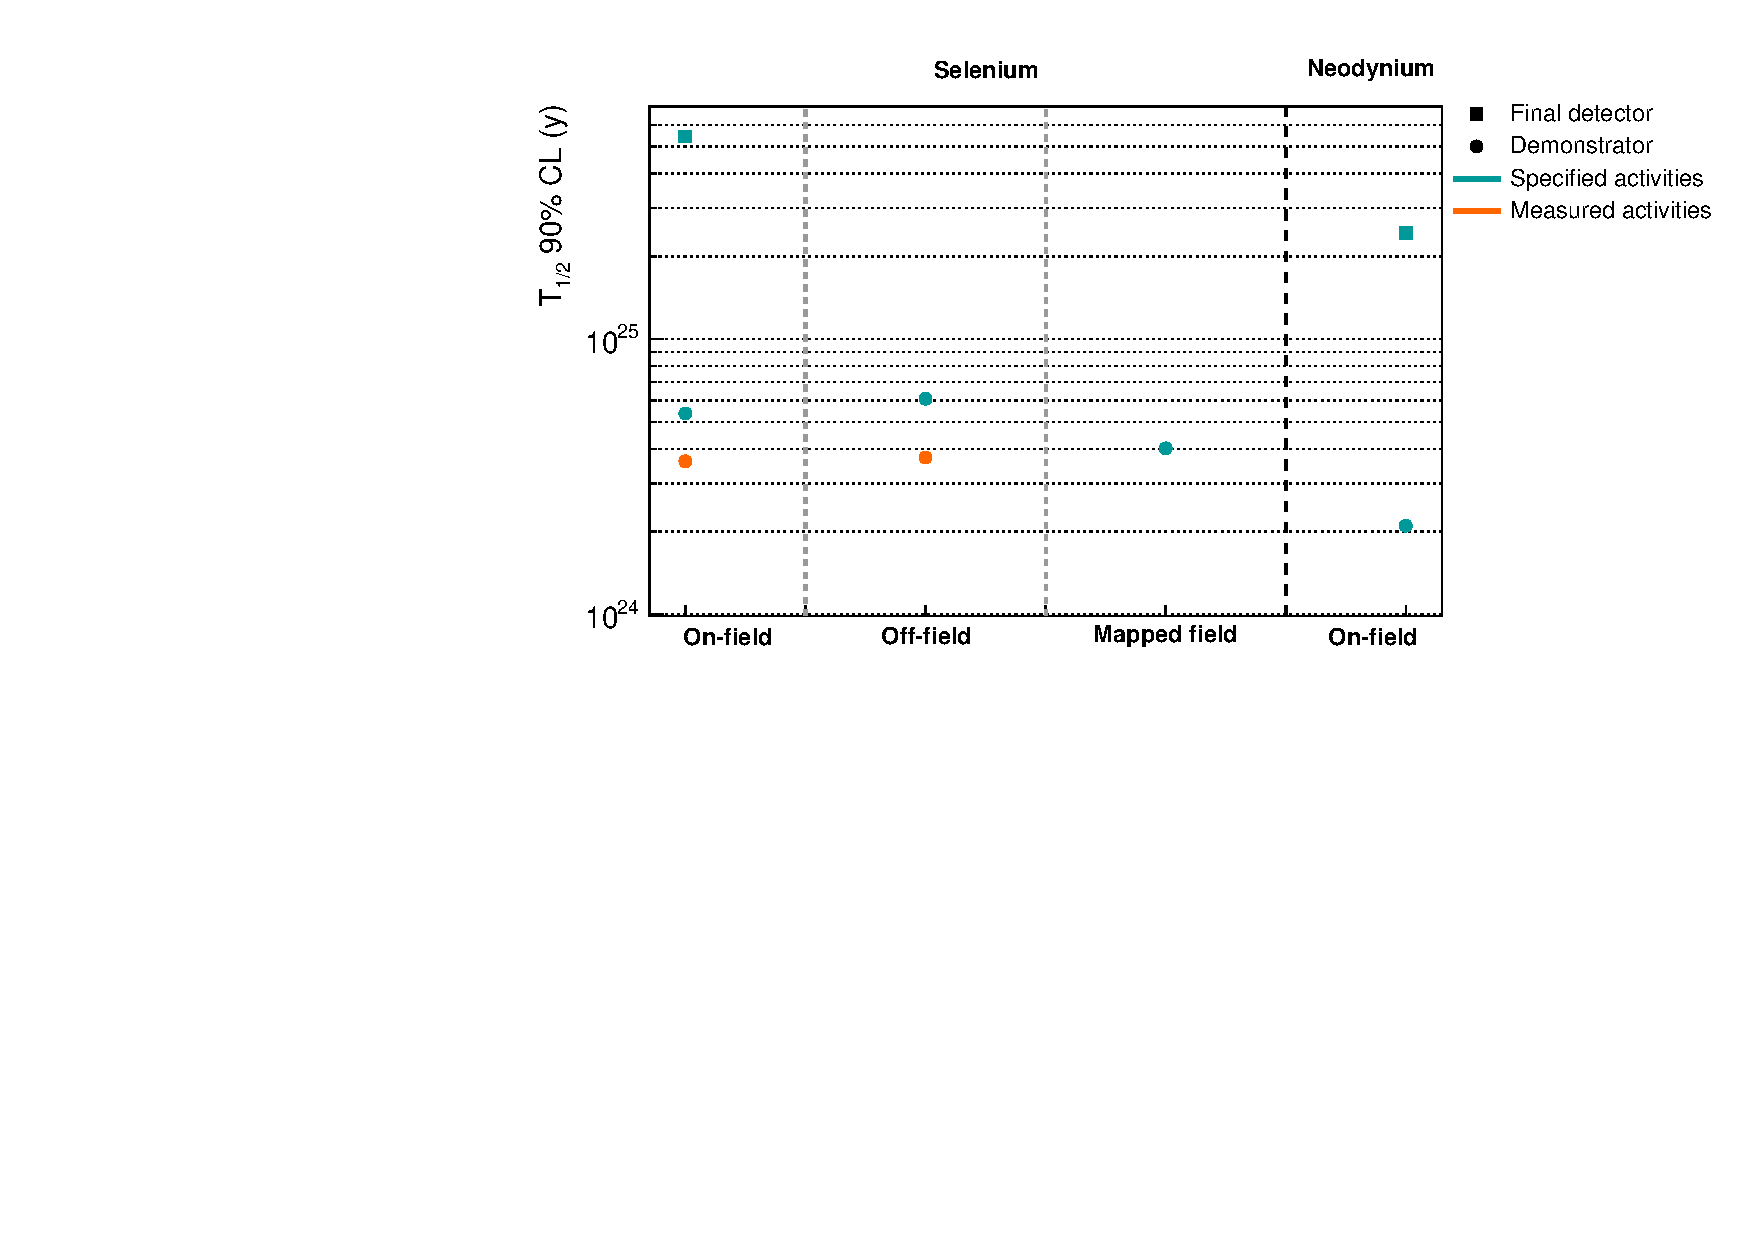
\includegraphics[width=1.1\textwidth]{Sensitivity/fig_sensitivity/final_t12.pdf}
%%   \caption{Summary of $\Tbeta$ $90$\% limits set.
%%     First-order and optimised topological cut-offs have been applied.
%%     Regions of interest have been optimised for each case.
%%     \label{fig:final_t12}}
%% \end{figure}
%% \begin{figure}[h!]
%%   \centering
%%   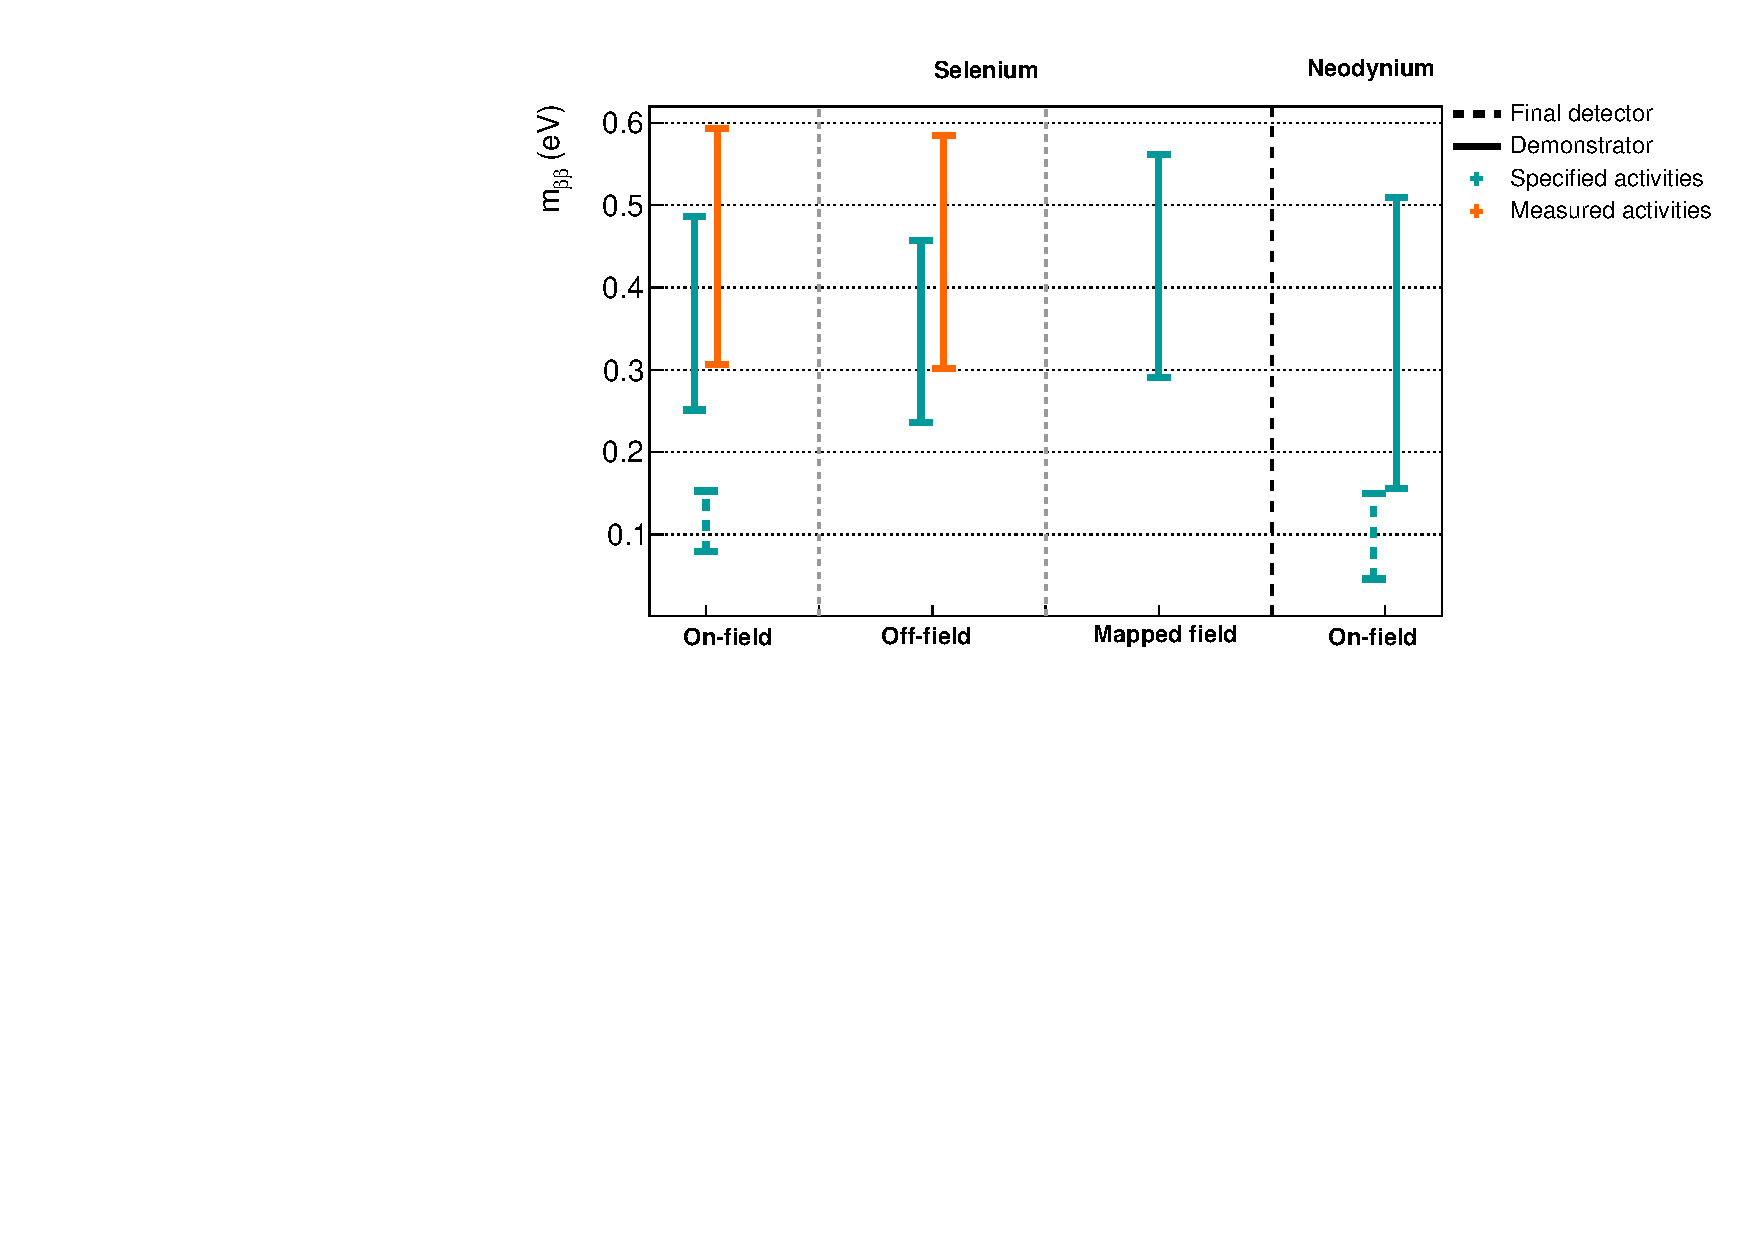
\includegraphics[width=1.1\textwidth]{Sensitivity/fig_sensitivity/final_mbb.pdf}
%%   \caption{Summary of $\mbb$ limits set.
%%     First-order and optimised topological cut-offs have been applied.
%%     Regions of interest have been optimised for each case.
%%     \label{fig:final_t12}}
%% \end{figure}

\begin{figure}[!h]
\centering
\begin{subfigure}[t]{1\textwidth}
  \centering
  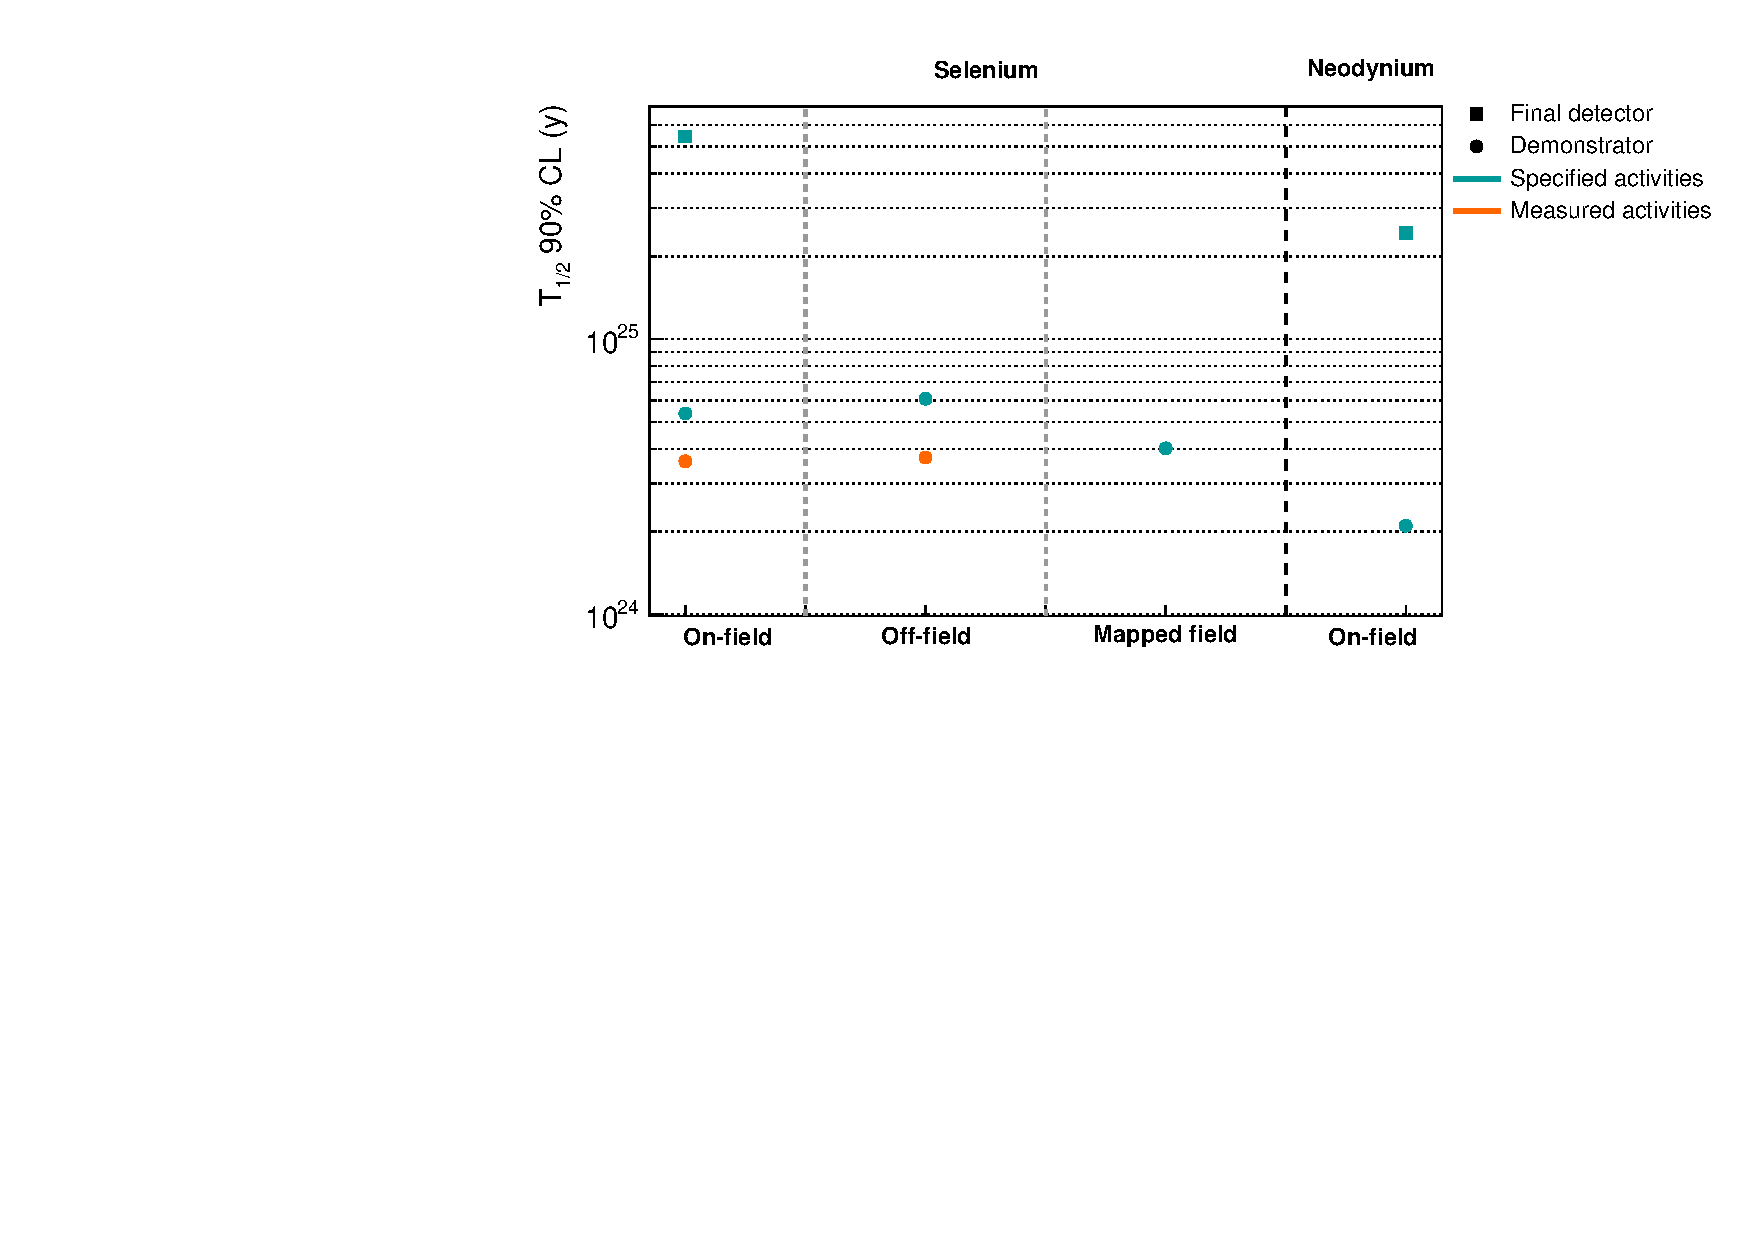
\includegraphics[width=1\textwidth]{Sensitivity/fig_sensitivity/final_t12.pdf}
  \captionsetup{justification=centering}
  \caption{$\Tbeta$ ($90$\% CL) limits.
    \label{subfig:summary_T12}}
\end{subfigure}
\vskip\baselineskip
\begin{subfigure}[t]{1\textwidth}
  \centering
  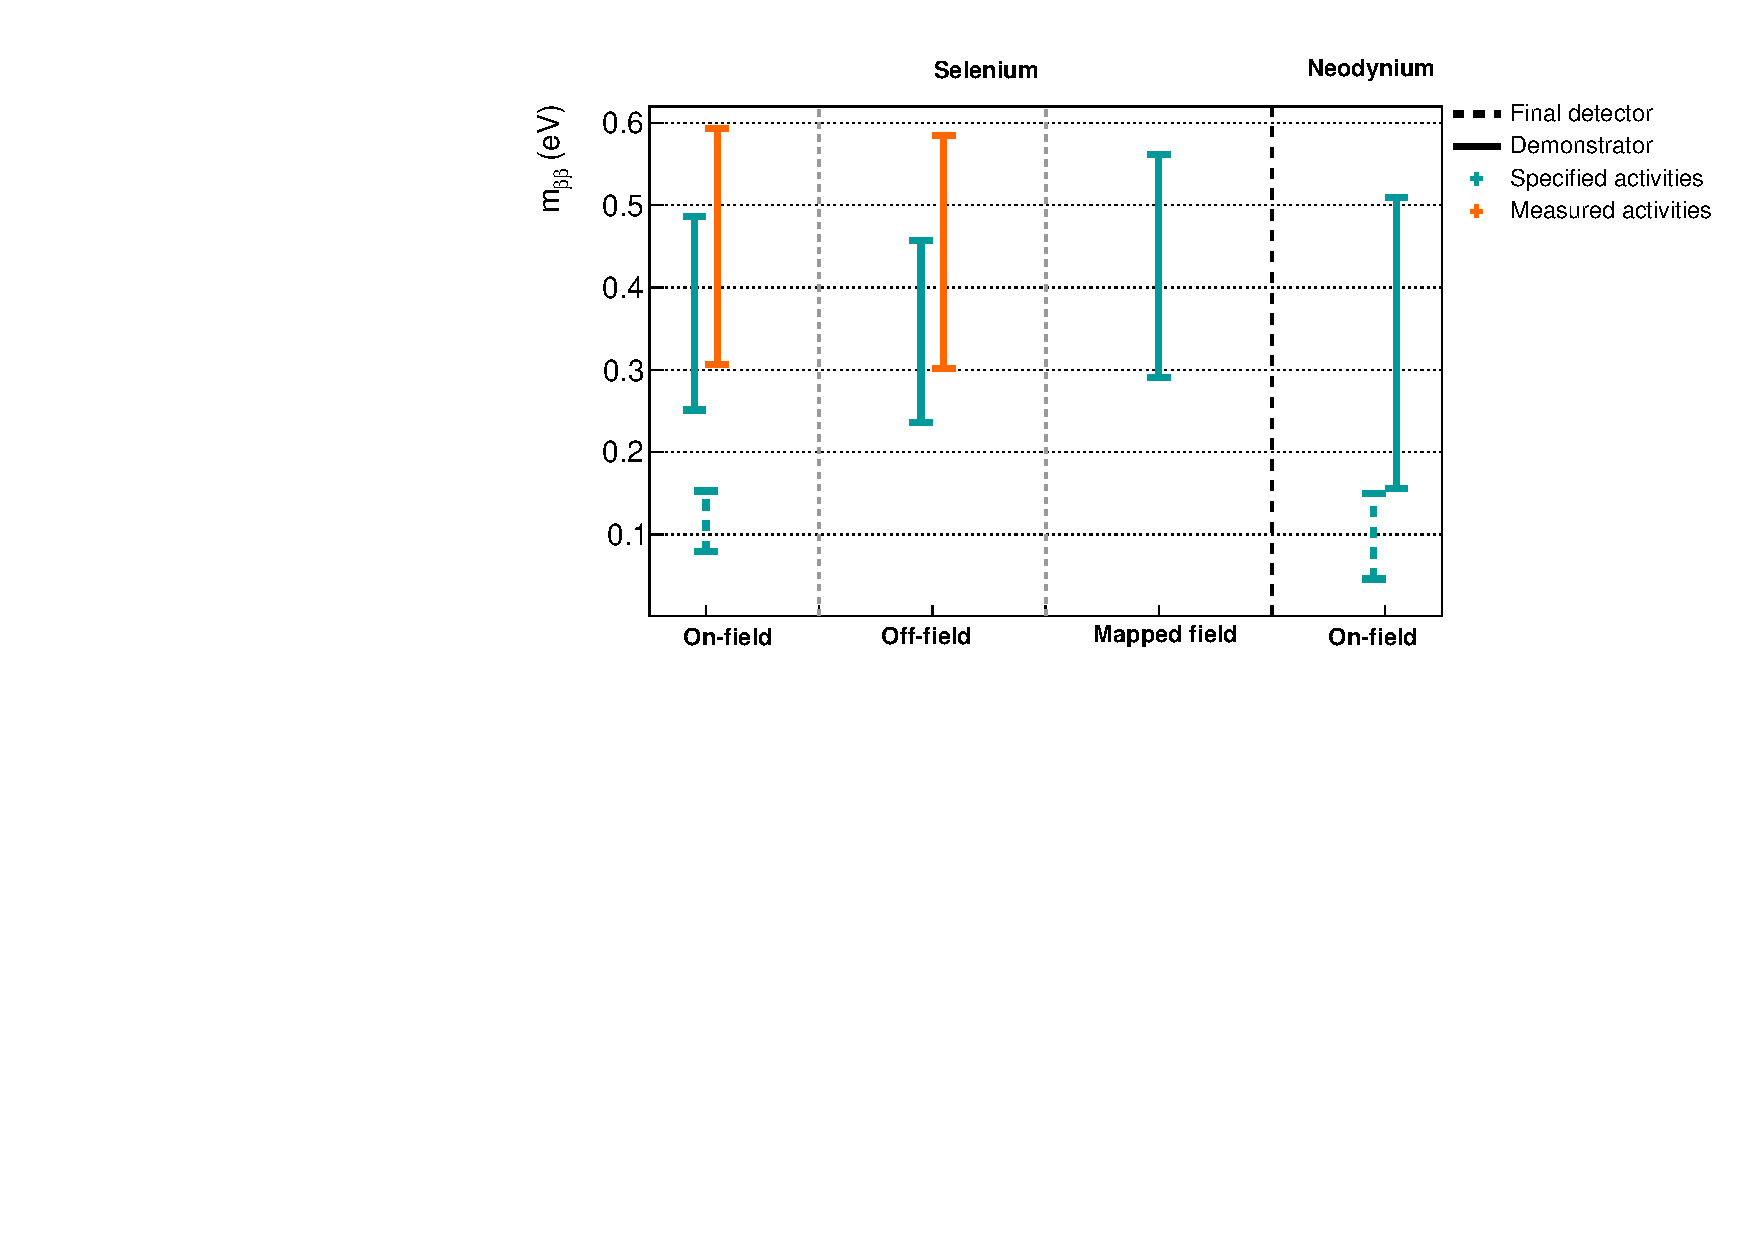
\includegraphics[width=1\textwidth]{Sensitivity/fig_sensitivity/final_mbb.pdf}
  \captionsetup{justification=centering}
  \caption{$\mbb$ limits.
    \label{subfig:summary_mbb}}
\end{subfigure}
\caption{Summary of limits set on $\Tbeta$ (a) and $\mbb$ (b) for each case dealt with in this chapter.
  First-order and optimised topological cut-offs have been applied.
  Regions of interest have been optimised for each case.
  \label{fig:final_t12}}
\end{figure}

               \chapter{Improvement of the rejection of the internal Thallium-$208$ background}
\label{ch:timediff}

At the end of September 2018, the Selenium-$82$ source foils were installed on the demonstrator.
At this time, the internal \Tl\ and \Bi\ activities had already been measured by the BiPo detector.
In this chapter, we focus on rejection techniques optimised to have a high efficiency on internal \Tl\ events.



\section{Motivations for this study}

We discussed in chapter~\ref{ch:sensitivity} about the specified levels of contamination inside the source foils.
These levels are embeded by the internal \Bi\ and \Tl\ activities, given in Tab.~\ref{tab:real_target_act}.
These specifications aimed at reaching the targeted \Se\ half-life limit of $\sim1\times10^{26}$~year for a $500$ kg/y exposure.
In the same table are also given the activities measured by the BiPo detector, after the sources production.
These measurements reveal a \Tl\ contamination, about $30$ times higher than expected.
As concluded in the previous chapter, this contamination impacts the sensitivity on the $\zeronu$ decay of the final detector, decreasing it.

In this section, we work to describe the specificities of Thallium-$208$ internal background.
We will see what the methods of rejecting this background already exist.
We will also detail the basic principle of a new method we have put in place, to meet the needs of rejections of Thallium, following the measurements of BiPo.

\subsection{The internal \Tl\ background}

Trace quantities of naturally-occurring radioactive isotopes inside the source foils can occasionally produce two-electron events, and thus can mimic $\beta\beta$-decay events.
The \Tl, a progeny of \U, is one of the largest contribution to the internal background.
In fact, two electrons can be produced via $\beta$-decay followed by a M\o{}ller scattering, $\beta$-decay to an excited state with the subsequent internal conversion, or due to Compton scattering of the de-excitation photon (Fig.~\ref{fig:internal_contamination}).
\begin{figure}
  \centering
  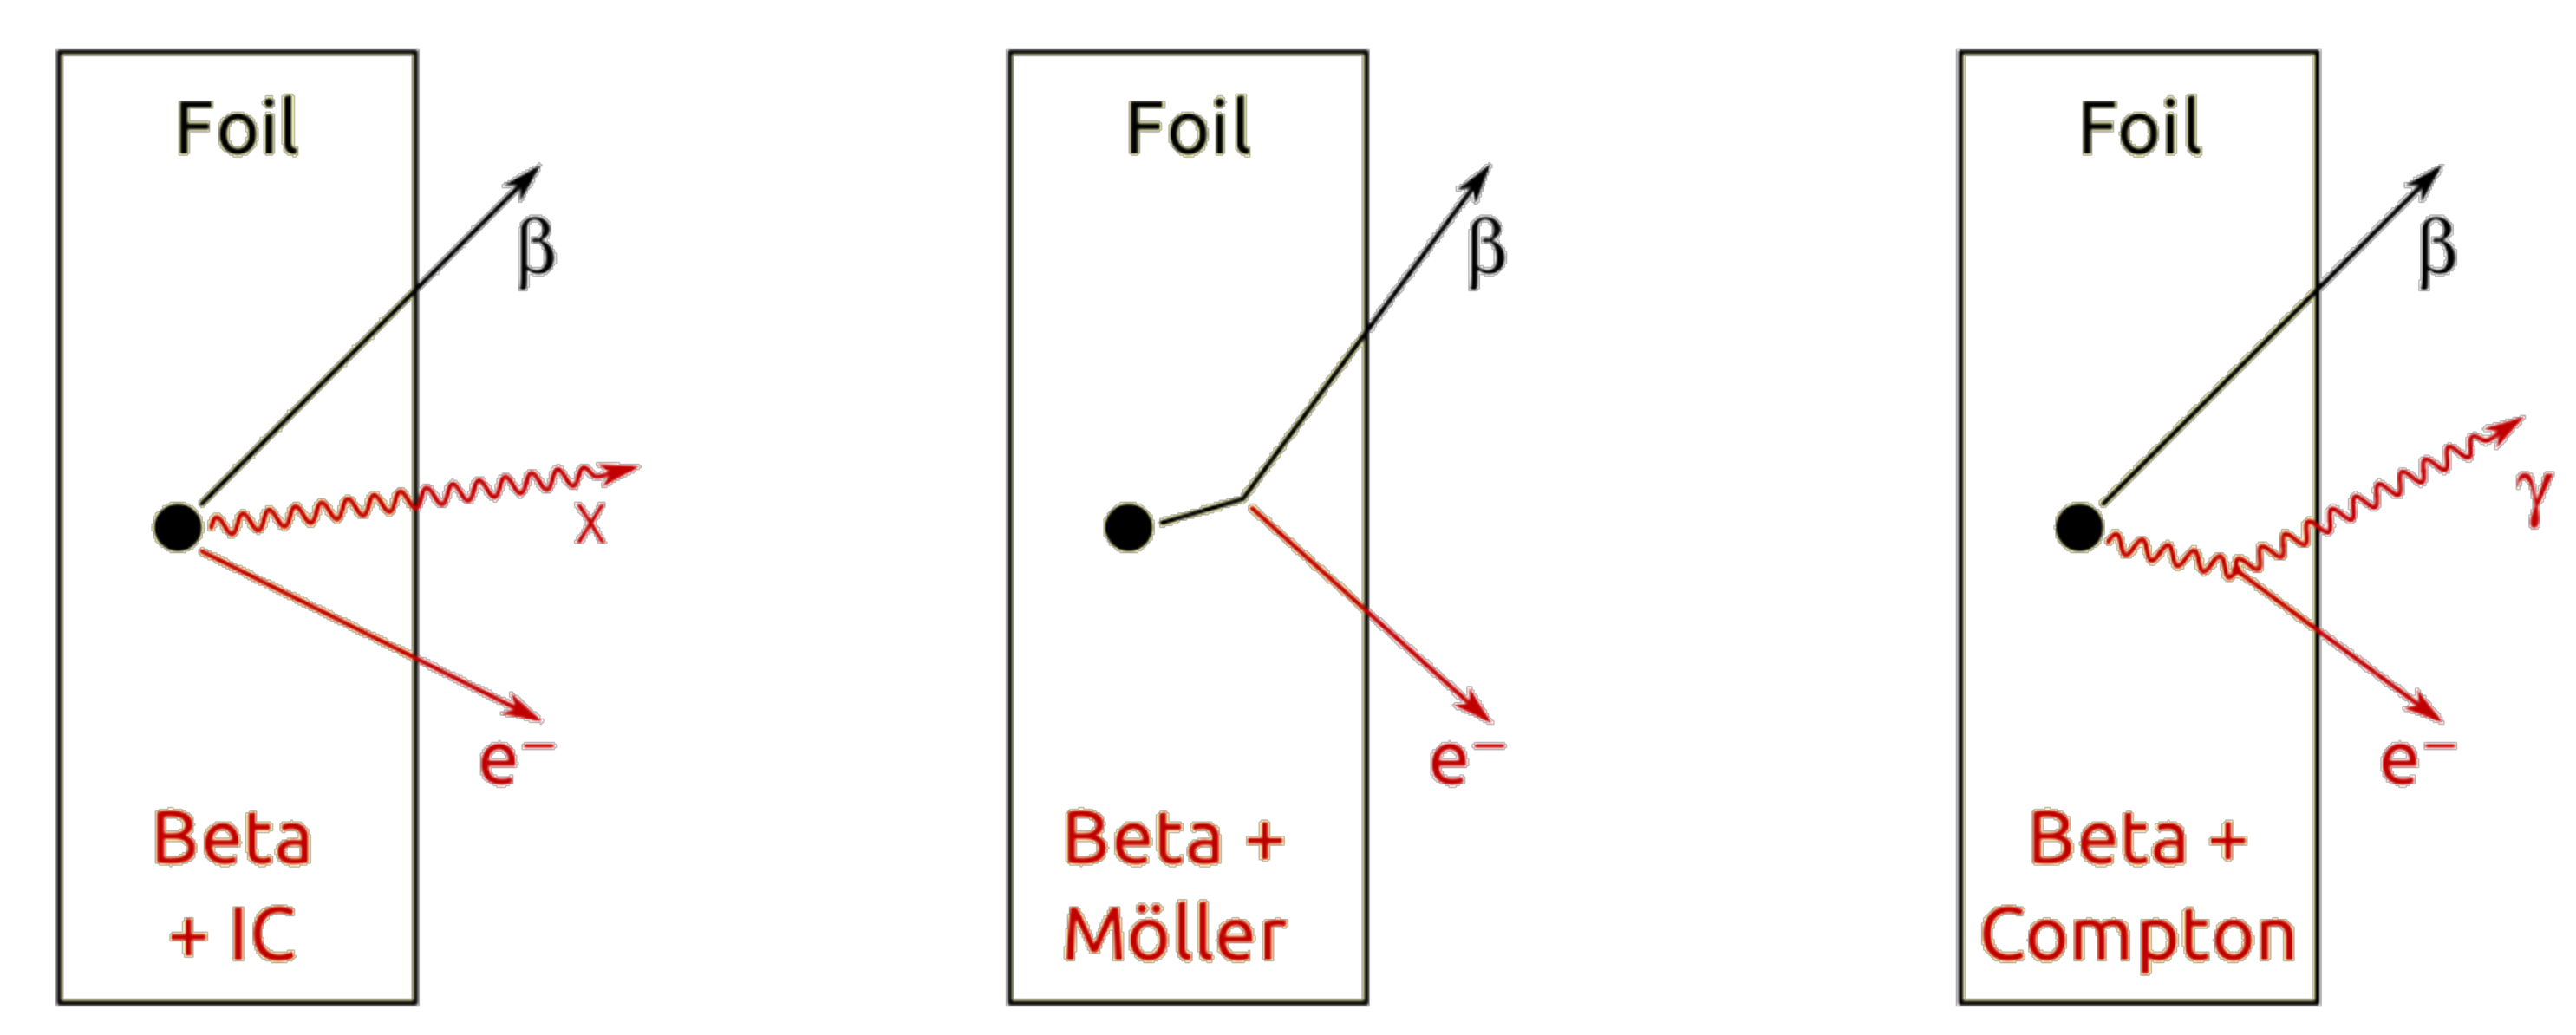
\includegraphics[width=10cm]{timedifference/fig_timediff/internal_contamination.pdf}
  \caption{(a) $\beta$ decay + internal convertion: \Tl\ nucleus performs a $\beta$ decay, then an electron is emitted after internal conversion of photon
    (b) $\beta$ decay + M\o{}ller:
    (c) $\beta$ decay + Compton diffusion: \Tl\ nucleus $\beta$ decays to an exited state, then the photon perfoms a Compton diffusion.
 \label{fig:internal_contamination}}
\end{figure}
%% The ultimate internal background for $\zeronu$ experiments is the $\twonu$ decay of the studied isotope.
%% When present in the source foils, \Tl\ and \Bi\ can mimic the $\zeronu$ signal by different processes (see Fig.~\ref{fig:internal_contamination}).

\subsection{Rejection of the \Tl\ background}
We present a simplified disintegration scheme of \Tl\ in Fig.~\ref{fig:Tl_scheme}.
\begin{figure}
  \centering
  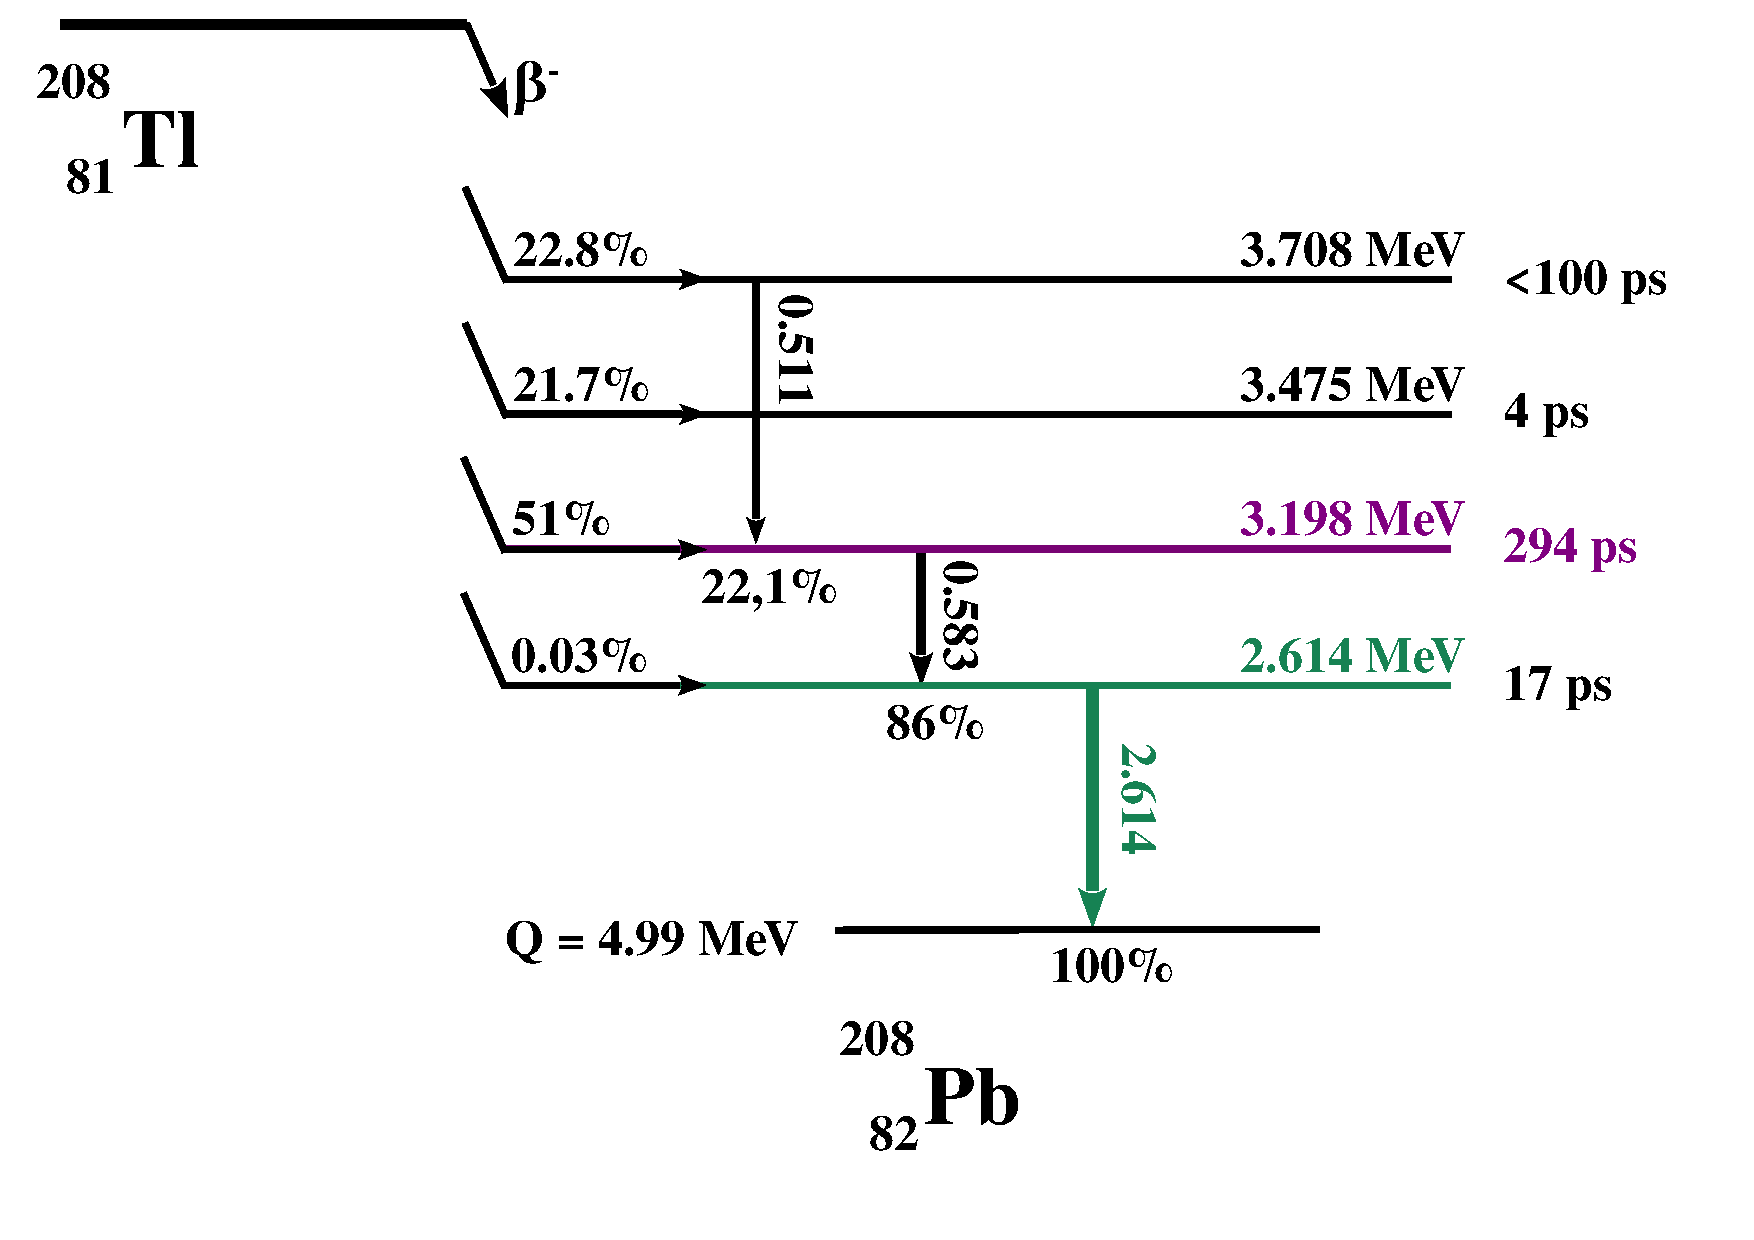
\includegraphics[width=13cm]{timedifference/fig_timediff/Tl_decay_scheme.pdf}
  \caption{Simplified desintegration scheme for \Tl\ isotope.
    The level in red has a significant life time of $294$ ps and can be useful in internal backgroung rejection.
  \label{fig:Tl_scheme}}
\end{figure}


For this study, we are focusing on the internal conversion process coming from the contamination of \Tl\ in the source foils.
Regarding the simplified desintegration scheme of the \Tl\ isotope (Fig.~\ref{fig:Tl_scheme}), we see that the $\beta$ desintegration has $51\%$ of probability to fall on the $294$ ps-life time exited level.
To decay to \Pb, the exited isotope has $100\%$ of probability to decay emmiting a $\gamma$ of $2.6$ keV.
In $0.2\%$ of cases, one of the orbital electron can interact with the exited nucleus and decay through internal conversion.
To summarise, decays where a \Tl\ nucleus emmits a $\beta$ particle and then an electron comming from internal conversion of the $2.6$ MeV-$\gamma$ represents $75\%$ of the total $\beta$ decays.
In this case, the internal conversion electron is time-delayed of $294$ ps compared with the $\beta$ particle.
We aim to use this delayed electron to discriminate \Tl\ internal background from signal and other internal backgrounds.





\begin{itemize}
\item trop de \Tl\ dans les sources par rapport aux spec
\item donc besoin d'une méthode de réjection spécifique pour \Tl\
\item pas gênant au niveau du démonstrateur (pour cela regarde le nombre d'événements de Tl208 attendus après l'optimisation des coupures avec le niveau de Tl208 mesuré par Bipo-3, je pense que c'est moins d'1 evt), mais cela peut être gênant pour une manip à 500 kg.y
\item avant de parler de la réjection avec le temps de vol, parler des autres réjections du Tl208 : bdf interne = 1 électron de conversion + 1 électron bêta -> l'électron de plus haute énergie a un pic en énergie (montrer une figure de simulation pour illustrer) et commenter avec le fait que la résolution en énergie s'améliore entre NEMO-3 et le démonstrateur. Donc normalement cette réjection sur l'énergie individuelle est plus efficace avec le démonstrateur.
\item Schema désintégration
\item Internal conversion -> reconnaître le Tl avec gamma $2.6$ MeV
\item Préciser l'énergie de l'électron de conversion associé (ou plutôt les énergies : raies K, L ...)
\item Un des deux gamma est retardé de 294 ps, puis conversion interne -> donner le proportion (nb d'ev attendus, dans la ROI)
\item Avant d'entrer dans le détail préciser le principe de la réjection par temps de vol.
L'électron de plus haute énergie est en retard, avec un retard en moyenne de 294 ps pour la plupart des niveaux (discuter un peu le schéma de désintégration, dans quel cas il sera en retard).
Ensuite dire que tu as quantifié le pourcentage d'électrons de haute énergie en retard avec une simulation "parfaite" i.e. avec une résolution en  temps  nulle.,
\end{itemize}

%% Internal conversion occurs after $\beta$ or $\alpha$ radioactive decays leaving the nucleus exited.
%% Then a $\gamma$ particle is emitted and transfers its energy to an atomic electron which results in ejection of this electron from the atom.
%% The emitted electron has an energy corresponding to the energy of previously exited nucleus reduced by the electron binding energy.
%% After the internal conversion, electrons reorganise.
%% The hole in internal layer is filled by an electron from an external layer (emitting an X ray).\\
%% The probability for an atomic electron to be ejected decreases with the initial binding energy.
%% Thus, electrons from K layers have a higher probability to be converted (see Fig.~\ref{fig:Tl_IC}).

\section{Describe mathematically internal events}

\subsection{The internal probability}
\begin{itemize}
\item outil déjà existant, déjà utilisé dans NEMO-$3$
\item identifier les ev venant de la source
\item détailler chaque terme
\item étudier l'influence du terme $\sigma_{l}$ dans la proba interne (on avait trouvé 0.03 ns pour avoir une Pint plate pour la 0nu)
\end{itemize}

\subsection{The exponential probability}
\begin{itemize}
\item besoin de décrire les ev conversion interne, avec une loi de probabilité
\item Avec un détecteur qui mesurerait parfaitement les temps et les énergies, la loi t(max) - t(min) serait une loi exponentielle, en pratique il faut la convoluer avec une gaussienne.
\item description de l'exponentially modified gaussian avec les paramètres des deux distrib (expo et gaus)
\item Ici montrer une distribution de Pexp pour des evts Tl208 (si possible aussi uniquement pour les evts Tl208 qui ont un Delta t(resolution parfaite) > 0
\item Decrire aussi comment on passe de la probabilité exponentielle modified gaussian à la probabilité cumulée, qui est celle sur laquelle tu vas couper.
\end{itemize}

\section{Event selection}
\begin{itemize}
\item cut Pint/Pexp
\item Montrer un biplot Pint/Pexp pour les evts Tl208 en représentant la coupure.
\item Optimisation of event selection: cut on delta t
\item 208Tl cut efficiency
\item cut efficiencies on 0nubb and other backgrounds
\item Donner le nb d'ev rejeté sur le nb d'ev total, puis sur le nb d'ev retardés
\end{itemize}

\section{Impact of \Tl\ rejection on the experiment's sensitivity}
Reprendre l'analyse de sensibilité faite avec Axel en rajoutant les cuts Pint/Pexp et delta t pour le final detector

\subsection{Influence of the calorimeter time resolution}
\begin{itemize}
\item Se servir des résultats de $\sigma_{t}$ trouvés au chap.~\ref{chap:Cobalt_study}
\item Mais dire que ces sigmas peuvent être améliorés
\item donc présenter l'évolution des résultats (efficacité de réjection et sensibilité) sur la réjection en fonction de la valeur de sigma t, à faire varier dans un certain range.
\item Tu pourrais avec une figure à 2D où tu montres l'efficacité relative 0nu (égale à 100\% avant cette coupure temporelle) en fonction de la réjection du Tl208 -> cela donne une courbe que tu parcoures et tu cherches à optimiser ton point de fonctionnement.
\end{itemize}


\section{Conclusions}




\begin{figure}
  \centering
  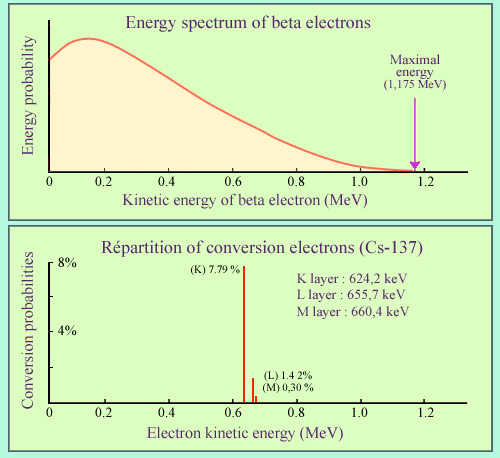
\includegraphics[width=9cm]{timedifference/fig_timediff/SpectreBeta_Cs137.jpg}
  \caption{\label{fig:Tl_IC}}

\end{figure}

               \chapter{Detector commissioning}
\label{ch:commissioning}

The commissioning of the SuperNEMO demonstrator has begun in $2019$ and first calorimeter data was taken.\\
The calorimeter of SuperNEMO is segmented in $712$ optical modules (OM), each composed by a coupling between a photomultiplier tube (PMT) and a polystyrene scintillator bloc (see Sec.~\ref{subsec:SN_calo} for more details).
The divider of a PMT is connected to $2$ cables, one providing the high voltage (HV), the other one, called signal cable, is a coaxial cable collecting and transporting the charge provided by the PMT.\\
By the summer $2020$, the SuperNEMO demonstrator will be encapsulated in an anti radon tent.
The so called \emph{patch panel} will insure passage of cables from the inside, to the outside of the anti radon tent, therefore doubling the amount of cables needed for the calorimeter.
We refer to the cables running from detector to patch panel as \emph{internal} cables, and the cables from patch panel to the electronic boards as \emph{external} cables.
Consequently, regarding only the calorimeter part, 2848 cables were cut, assembled, connector-mounted, transported and installed at LSM.
Then the check of every cable condition is mandatory to control and eventually fix them.

\section{Reflectometry analysis}
\label{sec:reflecto}

\subsection{Goal of the reflectometry analysis}

Taking into account the final demonstrator design, each coaxial length was determined, cables were cut and labelled in LAL, Orsay.
All external coaxial cables were designed to be $7$ meters-long -- the distance between electronic boards and patch panel being the same for all channels at electronic boards -- and internal cable lengths have been adapted to fit the distance from the patch panel to each optical module.
Then, cutting and labelling all cables lasted several weeks.
After all cables were transported and installed at LSM, we had to check each coaxial cable condition, for several reasons:
\begin{itemize*}
\item check if no cable was damaged during the transport and the installation;
\item control if no swap between cables has been made during cable labelling or calorimeter cabling,
\item check if the coaxial cable was cut at the right length,
\item more importantly estimate the signal time delay due to the cable lengths: knowing that the velocity of electrons in the coaxial cables has a known constant value, the longer is the cable, the more the signal takes time to travel from the PMT to the electronic channel.
  Therefore, each coaxial cable length has to be characterised, especially if we want to do time coincidences between two signals in two different channels.
\end{itemize*}
To do so, a pulse, called \emph{primary} pulse, is generated at the electronic board readout.
The signal will travel all along the coaxial cable, from the electronic board to the PMT divider.
Whether the cable is correctly connected to the PMT or not, the signal reflects at the other end.
\begin{figure}[h]
  \centering
  \begin{subfigure}[b]{0.3\textwidth}
    \centering
    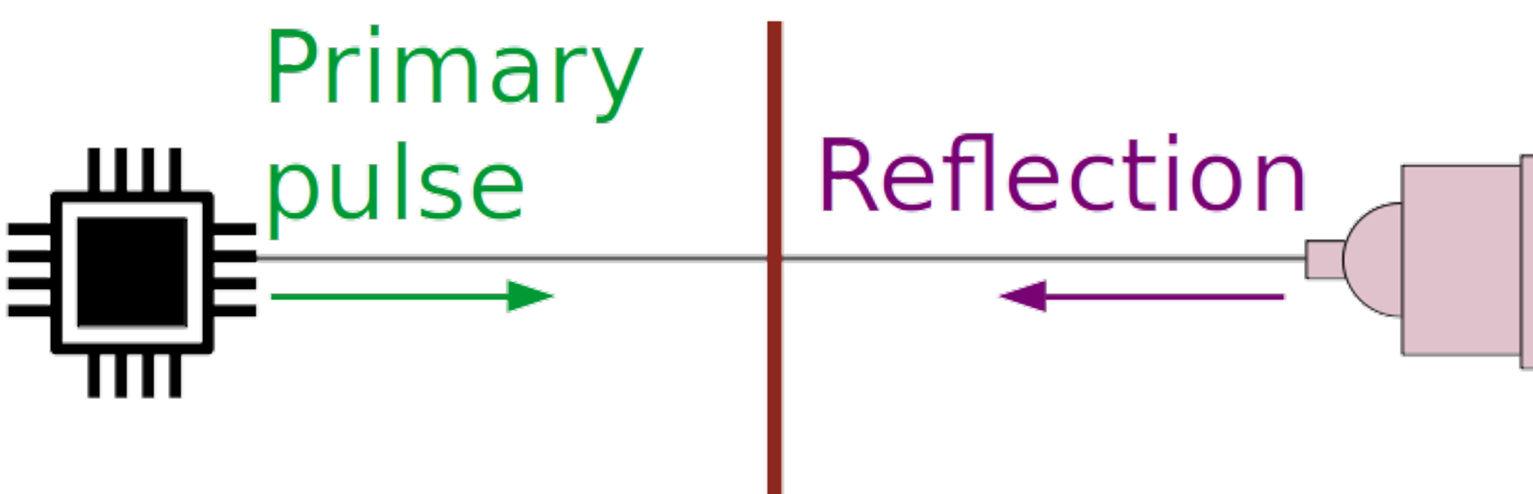
\includegraphics[width=1.1\textwidth]{commissioning/fig_commissioning/scheme_reflecto.pdf}
    \captionsetup{justification=centering}
    \caption{Normal reflection at PMT divider.
      \label{subfig:reflecto_normal}}

  \end{subfigure}
  \hfill
  \begin{subfigure}[b]{0.3\textwidth}
    \centering
    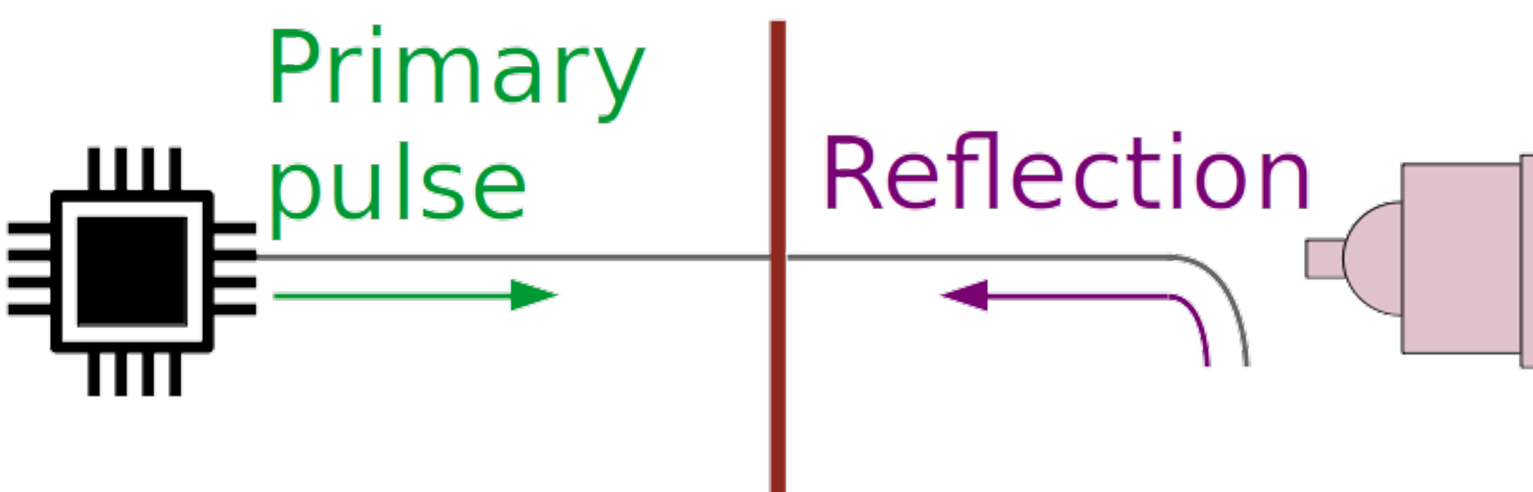
\includegraphics[width=1.1\textwidth]{commissioning/fig_commissioning/scheme_reflecto_1.pdf}
    \captionsetup{justification=centering}
    \caption{Cable not connected at PMT.
      \label{subfig:reflecto_pmt}}

  \end{subfigure}
  \hfill
  \begin{subfigure}[b]{0.3\textwidth}
    \centering
    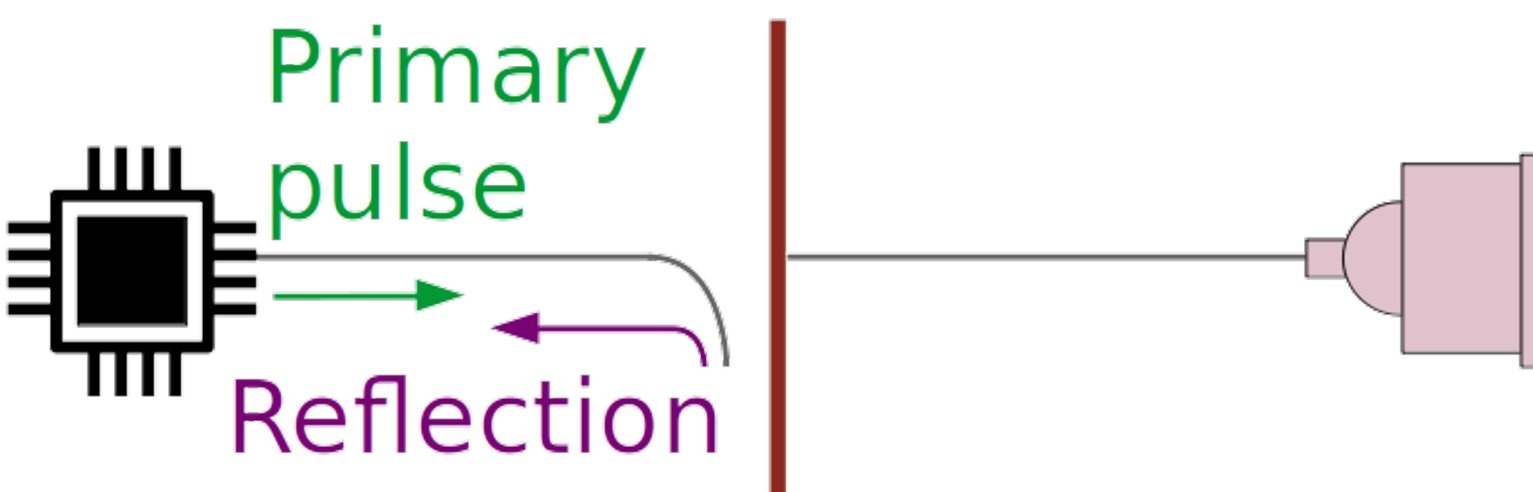
\includegraphics[width=1.1\textwidth]{commissioning/fig_commissioning/scheme_reflecto_2.pdf}
    \captionsetup{justification=centering}
    \caption{Cable not connected at patch panel.
      \label{subfig:reflecto_pp}}

  \end{subfigure}
  \caption{A representation of pulses sent in a cable for the reflectometry analysis is given.
    The electronic boards are symbolised by the black chip, and the patch panel by the red vertical bar.
    Three scenario where a primary pulse is sent in one cable (represented in grey), are represented.
    (a) The cable is well connected at the patch panel and at the PMT. The signal reflects at the PMT divider.
    (b) The cable is not connected at PMT and the signal is reflected at the end of the cable.
    (c) The cable is not connected at patch panel and the signal is reflected at the end of the external cable.\label{fig:reflecto_scheme}}

\end{figure}
Then the signal travels back from the PMT to the electronic board channel, where it is recorded by the acquisition.
We called this recorded reflected pulse \emph{secondary} pulse.
An example of the total recorded signal is displayed in Fig.~\ref{subfig:total_waveform}.
In order to accumulate enough statistics, we send thousands of pulses in each coaxial cable.
The analyses of the shape and of the arrival time of those secondary pulses for each channel is called \emph{reflectometry}, and allow us to check the coaxial cable conditions and to control their lengths.

\subsection{Pulse timing: controlling cable lengths}
\label{subsec:timing}

The first step of this analysis is to experimentally determine the length $l_{j}^{m}$ for all signal cables $j$ installed on the demonstrator.
This length is defined as
\begin{equation}
  l_{j}^{m}= 0.5\,t_{j}\,v_{p}\, ,
\end{equation}
where $t_{j}$ stands as the time made by the electrons to do a round trip between one electronic channel and one PMT, and $v_{p}$ is the velocity of electrons in the coaxial cables, which can be expressed as a fraction of light speed in vacuum, $c$.
The time difference $t_{j}$ between the primary pulse and the secondary pulse is written as
\begin{equation}
  t_{j} = \braket{t_{\text{secondary pulse}}-t_{\text{primary pulse}}}_{p} \, \text{,}
\end{equation}
$\braket{}_{p}$ being the average over all pulses sent in one single cable $j$.
The velocity $v_{p}$ is supplied by the cable manufacturer as
\begin{equation*}
  v_{p}=\frac{c}{\sqrt{\epsilon_{r}}}\,\text{,}
\end{equation*}
with $\epsilon_{r}$ the relative dielectric constant of the material.
Therefore, this celerity depends on the components.
For the coaxial cables chosen in the demonstrator design, the data sheet of the cable gives ${v_{p}=0.69\,c}$.
A study is performed to verify experimentally the value of $v_{p}$.
Three cables of different lengths are measured with a precision of $1$ cm.
A thousand of primary pulses are sent in each of the three cables, then the time for each secondary pulse is recorded.
At the end, we have three independent measures of the velocity $v_{p}$ in the used coaxial cables.
In Fig.~\ref{fig:celerity} is displayed the lengths $l_{j}$ as a function of the times $t_{j}$.
\begin{figure}[h]
  \centering
  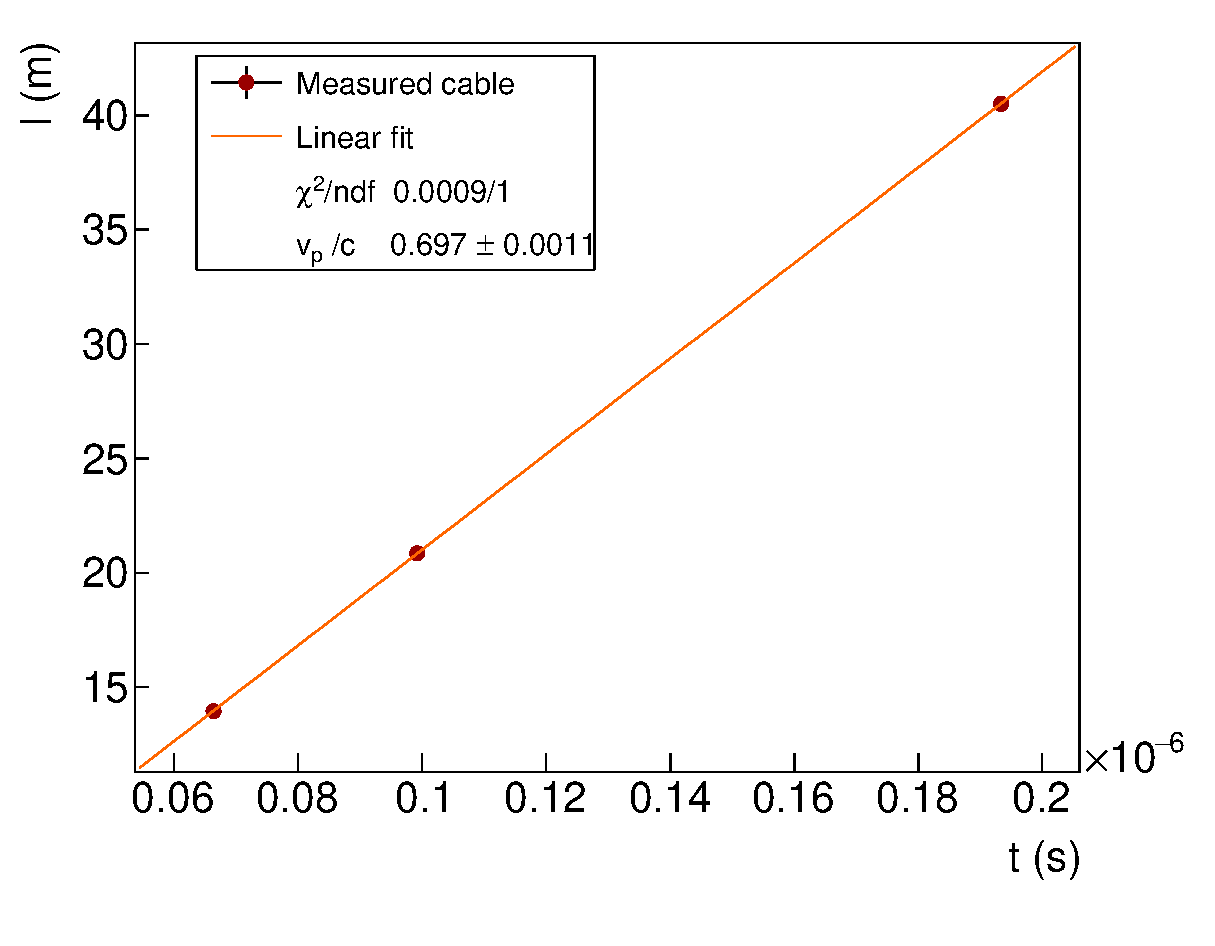
\includegraphics[width=15cm]{commissioning/fig_commissioning/celerity.eps}
  \caption{Three different lengths $l_{j}$ of cables are measured.
    Pulses are sent inside all cables.
    The lengths $l_{j}$ are plotted as a function of the time differences $t_{j}$ between primary and secondary pulses.
    The value of $v_{p}/c$ fitted from the data points is displayed.
    This value of $0.697\pm 0.0011$ shows the compatibility with the one supplied by the constructor, of $0.69$ c.
    \label{fig:celerity}}
\end{figure}
The fitted value of $v_{p}/c = 0.697\pm 0.0011$ is displayed and shows a compatibility up to $7\sigma$ with the data sheet.

As we want to determine the time interval $t_{j}$, we have to define what is the \emph{time} of a pulse.
In this analysis, we use a technique called Constant Fraction Discriminator (CFD), providing an amplitude-independent information about time of a pulse.
This algorithm aims at tracking a signal and defining its time arrival at a given fraction $f$ of its maximal amplitude.
The two main advantages of this technique is that it provides an efficient rejection of the noise in the acquisition window, and gives a good resolution on the measured time.
Nevertheless, the possible influence of the chosen value for the $f$ parameter on this time resolution has to be investigated.
We perform such a study in Sec.~\ref{subsec:CFD}.
We concluded that the highest precision on the time measurement arises for $f = 40\%$, and we adopt this value for the following analysis.
A graphic representation of the CFD time search is given in fig.~\ref{subfig:zoom_secondary}.
\begin{figure}[h]
  \centering
  \begin{subfigure}[t]{0.7\textwidth}
    \centering
    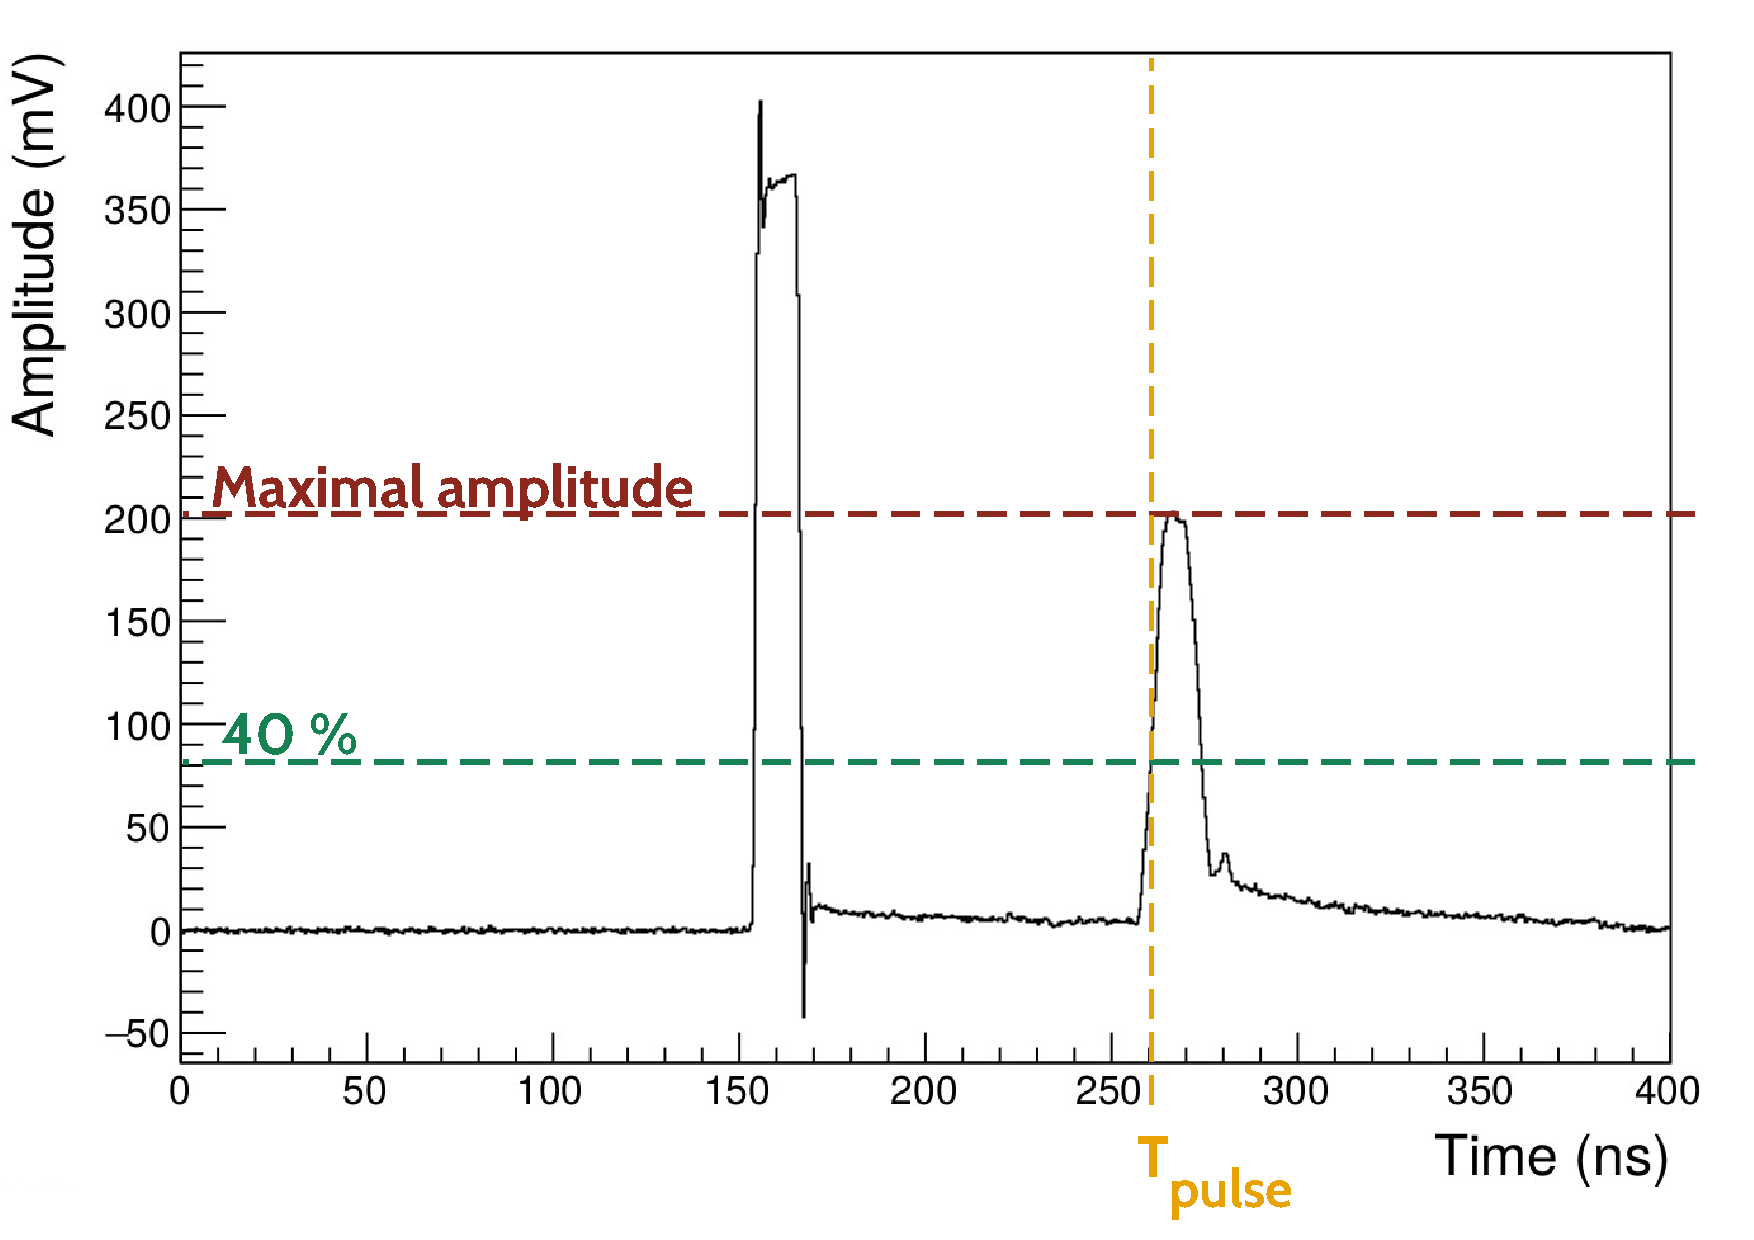
\includegraphics[trim={1.2cm 3.5cm 1.7cm 3.1cm},clip,width=1\textwidth]{commissioning/fig_commissioning/CFD_example.pdf}
    \captionsetup{justification=centering}
    \caption{Total recorded waveform
      \label{subfig:total_waveform}}
  \end{subfigure}
  \hfill
  \begin{subfigure}[t]{0.7\textwidth}
    \centering
    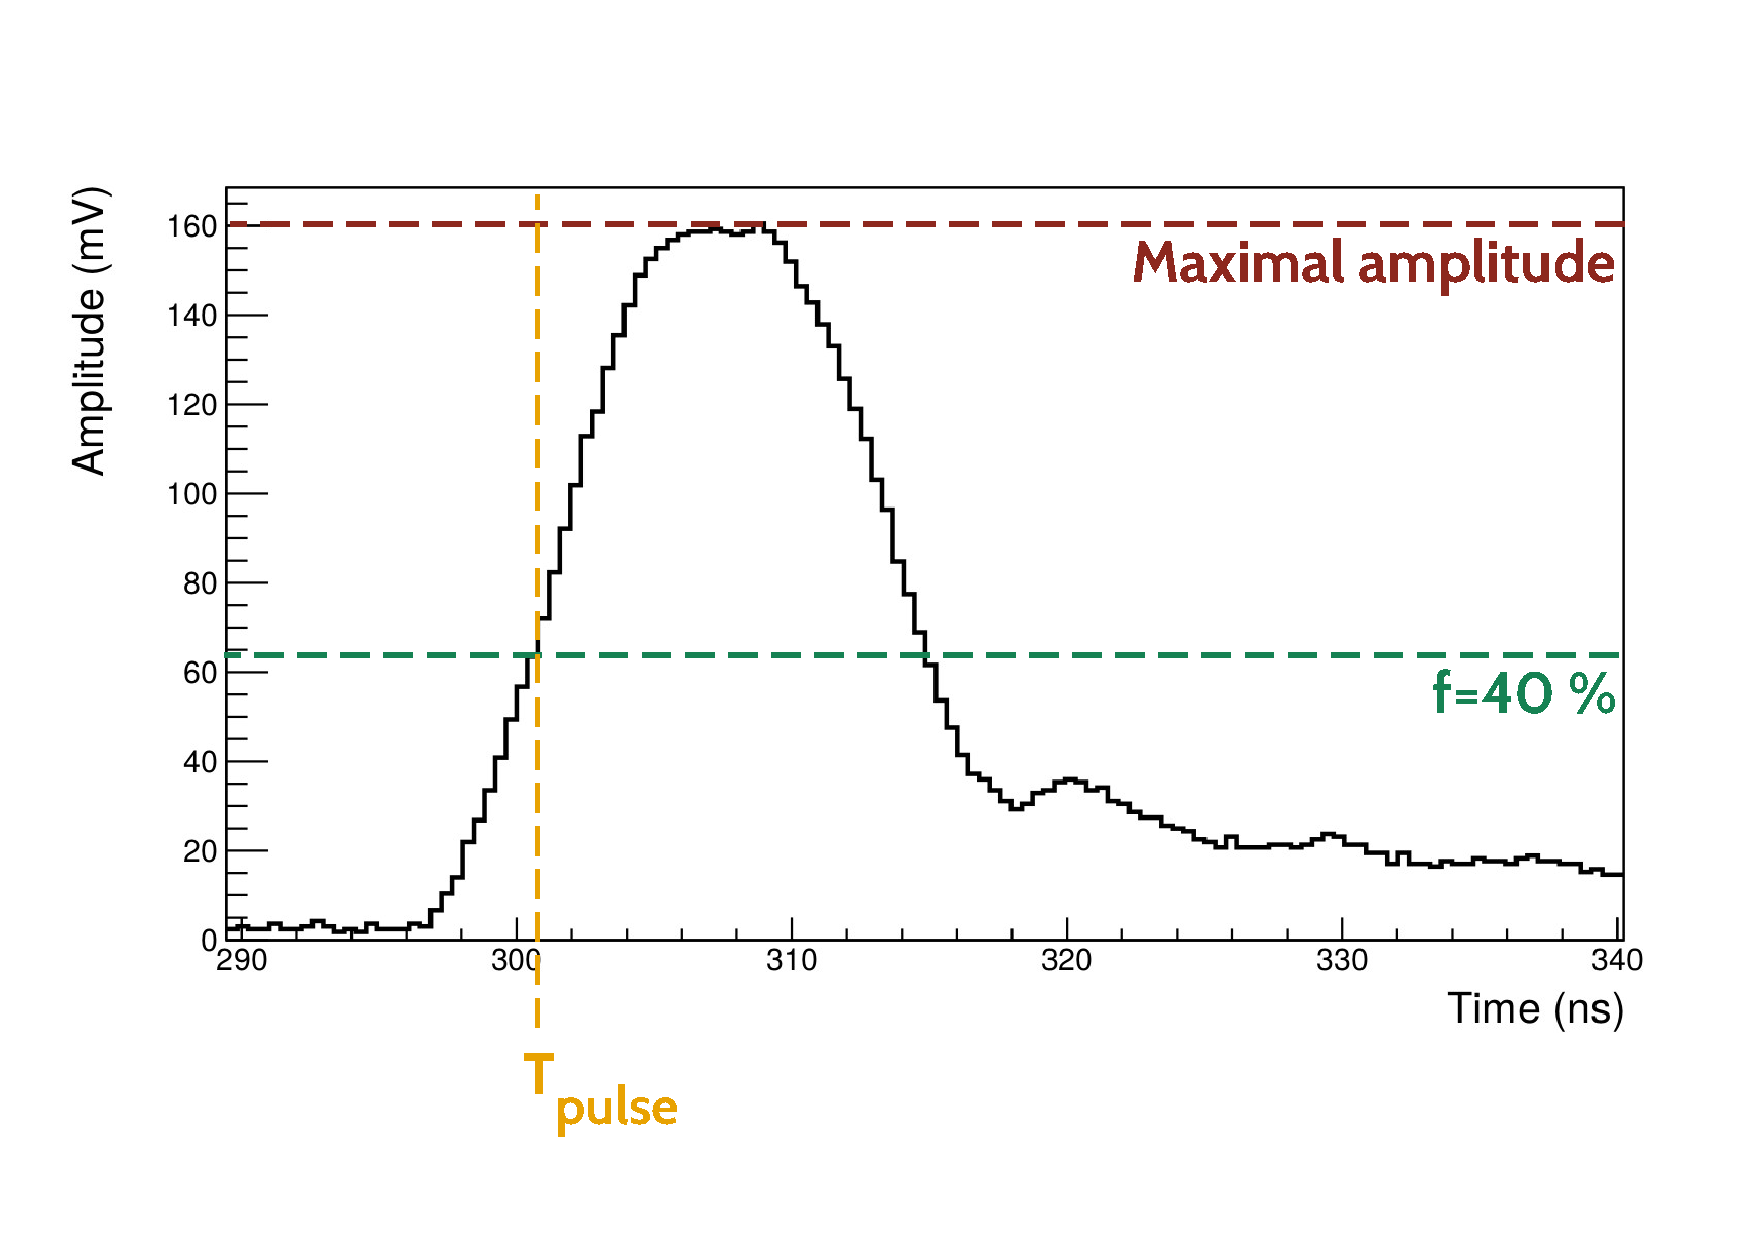
\includegraphics[trim={1.2cm 1.5cm 1.7cm 3.1cm},clip,width=1\textwidth]{commissioning/fig_commissioning/CFD_example_zoom.pdf}
    \captionsetup{justification=centering}
    \caption{Zoom on secondary pulse
      \label{subfig:zoom_secondary}}
  \end{subfigure}
  \caption{(a) Total recorded waveform: primary pulse (left) and secondary the pulse (right).
    (b) Zoom on the secondary pulse.
    A representation of time computed with a Constant Fraction Discriminator (CFD) is provided.
    Its maximal amplitude (red dotted line) and its fraction for $\text{f}=40\%$ (green dotted line) are displayed.
    The time $\text{T}_{\text{pulse}}$ (orange dotted line) represents the time of arrival of the secondary pulse computed with CFD, with the fraction $\text{f}=40\%$.
    \label{fig:CFD}}
\end{figure}
As we want to measure the installed cable lengths $l^{m}_{j}$, and compare them to the initially designed ones, $l^{d}_{j}$, we define the length difference $\Delta L_{j}$ as:
\begin{equation}
  \Delta L_{j} = l^{m}_{j}-l^{d}_{j}\, .
\end{equation}
In Fig.~\ref{fig:LengthDiff} is displayed the distribution $\Delta L$ for all the measured lengths.
\begin{figure}[h]
  \centering
  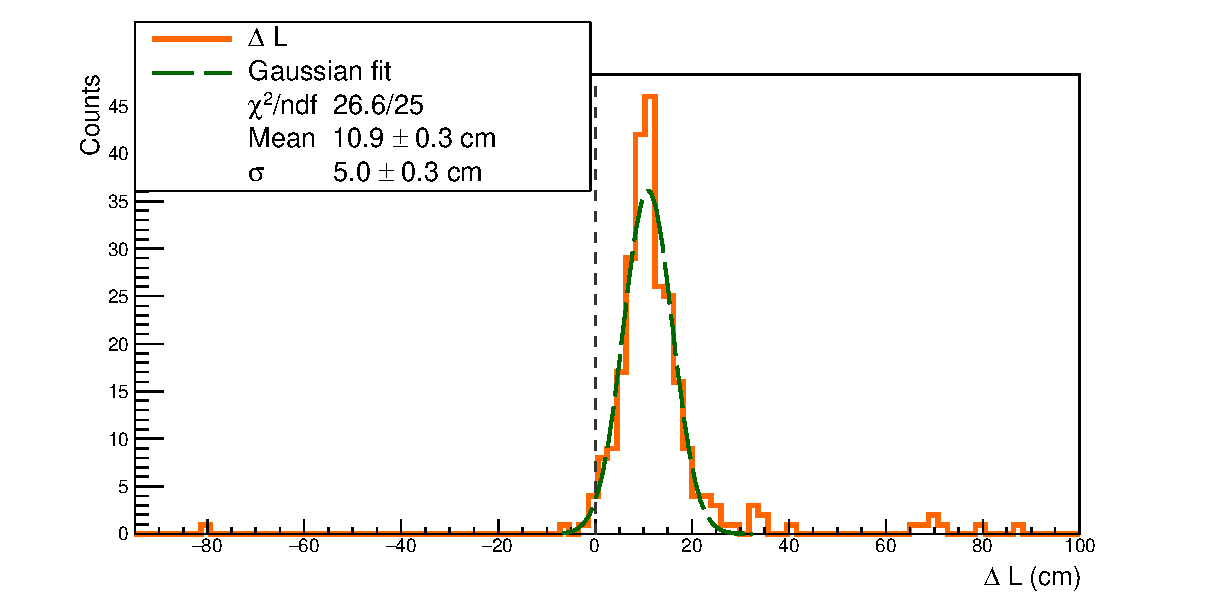
\includegraphics[width=15cm]{commissioning/fig_commissioning/length_diff.eps}

  \caption{The distribution of difference between the measured lengths $l^{m}$ and the expected lengths $l^{d}$ is displayed in orange solid line.
    The black dashed line represents the case where $l^{m}_{j} = l^{d}_{j} \;\forall j$.
    The Gaussian fit (green dashed line) presents a mean of $10.9 \pm 0.3$ cm.
    Some data points considered as outliers are beyond $3\sigma$.
    \label{fig:LengthDiff}}
\end{figure}
In hypothetical perfect conditions, all the cables should fit the design length, in other words, $l^{d}_{j} = l^{m}_{j}$.
Consequently the $\Delta L$ distribution should a peak at zero, as materialised by the black dashed line.
However, in real conditions, the measured length can be different from the designed one, leading the $\Delta L$ distribution plotted in orange solid line.
We conclude that the observed cable length $l^{m}$ differs from $l^{d}$ by $+10.9\pm 0.3$ cm, meaning that cables are longer than expected in average.
This may reveal a bias coming from the device used to cut the cables.
In fact, during cable cutting work, we noticed that the cutting device had a tendency to slip, probably leading to cables with extra lengths.
We assumed the cutting device has a given probability to slip for one meter of cable.
If this is the case, the probability for the device to give extra length should increase with the cable length.

To verify this assumption, we plot in Fig.~\ref{fig:CutBias} the length difference $\Delta L$ as a function of the initial design length $l^{d}$ (cyan).
From those data points, we compute a linear fit (orange solid line), parameterised as $y = \alpha x + \beta$, revealing that the cutting device presents two different biases.
\begin{figure}[h]
  \centering
  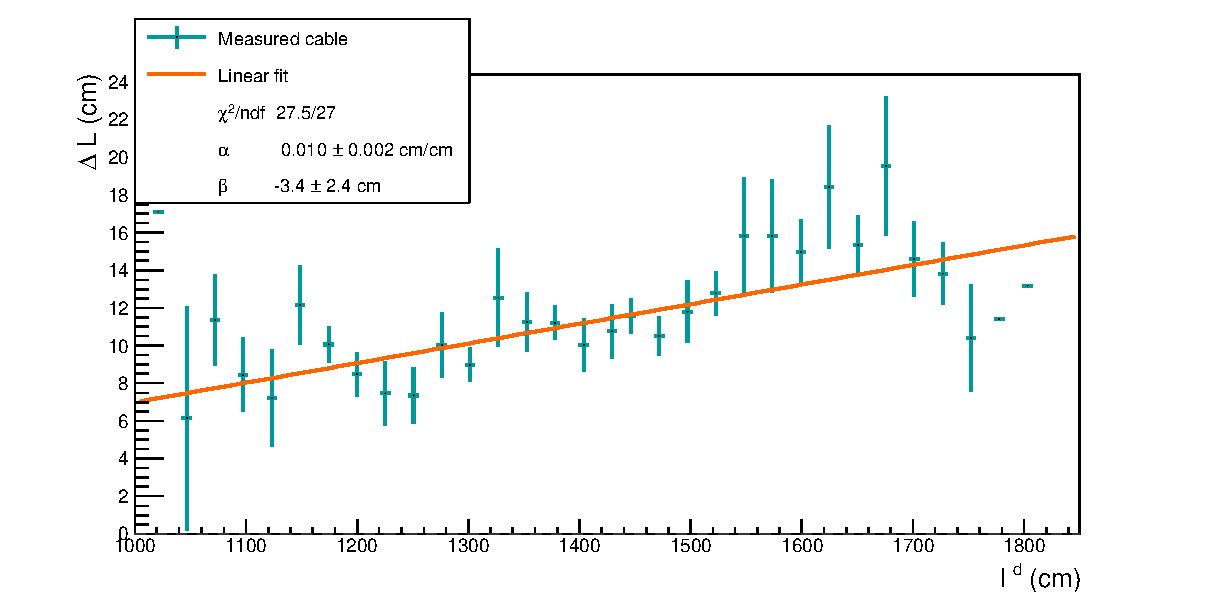
\includegraphics[width=15cm]{commissioning/fig_commissioning/cut_biais.eps}

  \caption{$\Delta L$ is plotted with $l^{d}$ (cyan), where $l^{d}$ is averaged for all the lengths designed to have the same value, being at the origin of vertical error bars.
    In black dashed line is represented the case where $l^{m} = l^{m}$.
    Data points are fitted by $\alpha x + \beta$, with $\alpha > 0$ and $\beta < 0$, revealing the two biases of the cutting device.
    \label{fig:CutBias}}
\end{figure}
The value of $\beta$ shows that the cutting device systematically took away $3.4$ cm of each cable.
Nevertheless, as the shortest cable was designed to be 10 meters long, there are no important consequences of this bias on the length difference $\Delta L$.
Besides, the slope $\alpha = 0.010\pm 0.002$ of the linear fit reveals that the cutting device adds one centimetre for every meter of cable, being compatible with the hypothesis on the cutting device sliding.
Hopefully this bias is not problematic as it makes most of the actual cable lengths longer than the design, while shorter lengths could have led to systematic connection issues to PMTs.
However, we notice that a few cables have been cut too short by mistake, the worse of them being $80$ centimetres shorter than expected.
Fortunately, this cable  was successfully connected to PMT despite this deficit.
On the contrary, few cables have a large extra length.
This probably is due to human punctual mistakes on top of the observed bias, but without any strong consequences for the calorimeter operation.
In conclusion, no important mistakes have been made when cutting cables, and we had no issue for connecting the only problematic cable.

If the main goal of this study is to check the lengths of coaxial cables, it also aims at correcting the time of recorded events, from the time made by the signal to travel from a PMT to an electronic channel.
taking into account the time for the signal to travel through cables.
This become possible with the reflectometry study we performed.
Knowing real lengths of cables and using the celerity of the signal, we deduce the time needed for the signal to travel from one given PMT divider to the electronic boards.
Then we can correct event times.

As explained previously, the time $t_{j}$ gives information about the length of the cable $j$.
We remind the coaxial cables are divided in two parts, one external and one internal, both linked by the so-called patch panel.
Thus we can use that travel time to detect possible disconnection of a cable at patch panel.
In fact, if one cable is not connected at the patch panel -- this case is illustrated in Fig.~\ref{subfig:reflecto_pp}, -- the pulse reflects at the end of the external cable part, going back to the electronic board.
This very short time, giving information about the location of the reflection, is used to tag a patch-panel disconnection.
Then, a simple check onsite can confirm this observation, and the external part of the cable can be connected to the patch panel.\\

This study allowed us to control and record the lengths of all coaxial cables installed on the SuperNEMO demonstrator at LSM, and gave information on the status of cable connections at patch panel.
We also have understood the main results on measured cable lengths and the functioning and biases of the cutting device that we used.

\subsection{Signal attenuation}
\label{subsec:attenuation}
The attenuation of an electric signal is a problem common to all electronic fields, and comes from the charge loss of an electromagnetic wave travelling in a medium.
%% Then, another test for controlling the cable condition is to check if this attenuation matches
%% the expectations (i.e. the attenuation per metre of cable given by constructor).
%% The signal attenuation car be define in two different ways:
%% \begin{itemize*}
%% \item using the signal amplitude ratio
%% \end{itemize*}
For a coaxial cable, this attenuation mainly depends on the signal frequency $f$ in MHz and on the cable characteristics.
For the coaxial cables, the theoretical linear attenuation $\alpha_{\text{att}}^{\text{th}}$, so be it the attenuation by metre of cable in dB/m, is supplied by the constructor as
\begin{equation}
  \alpha_{\text{att}}^{\text{th}} = f\sqrt{\epsilon}(\frac{a}{\sqrt{f}}+b)\,,
\end{equation}
where the factor $a$ depends on the diameter of the dielectric material on one side, and of the diameter of the conductor material on the other side, and where $b$ is function of the dielectric loss factor, characterising the material's dissipation of electromagnetic energy.
For the used coaxial cables, and with a frequency $f$ of few GHz for the signal pulses sent in cables, we calculate this attenuation as $\alpha_{\text{att}}^{\text{th}} = 1.22$ dB/m.
In a more general manner, the attenuation of a signal in dB is defined with the decimal logarithm of a power ratio.
We use this definition to determine the attenuation in the framework of the reflectometry analysis, defining the attenuation $\mathcal{A}$, for a given length of cable $l$, as
\begin{equation}
  \mathcal{A}=10\log_{10}\frac{V_{\text{primary pulse}}}{V_{\text{secondary pulse}}} \,\text{,}
\end{equation}
where $V_{i}$ is a quantity representing the intensity of the signal.
$V$ can correspond to the maximal amplitude of the pulse, as well as the \emph{integrated charge} of the pulse, defined as the amount of current received by the acquisition over a given time window.
As the provided data sheet does not specify the attenuation of which quantity (amplitude or charge) represents $\alpha_{\text{att}}^{\text{th}}$, we decide to investigate both in the following.
Then, we define the linear attenuation $\alpha_{\text{att}}^{\text{R}}$, measured by reflectometry in dB/m, with
\begin{equation}
  \mathcal{A} = f_{r}+\alpha_{\text{att}}^{\text{R}}\,l\,,
\end{equation}
with $f_{r} = -10\log_{10}R$, where $R$ is the reflection factor characterising the pulse reflection on the PMT divider.
In fact, as the circuit is opened, the pulse is reflected at the PMT divider, but only partially.
A part of the signal is not reflected but lost through the divider.
This reflection is characterised by $R$, which is function of the impedance $Z_{c}$ of the cable, and of the impedance $Z_{d}$ at the divider level, where the pulse is reflected.
It is written as
\begin{equation}
  R = \frac{Z_{d}-Z_{c}}{Z_{d}+Z_{c}}\,,
\end{equation}
where we have the limit
\begin{equation}
  \lim_{Z_{d} \to \infty} f_{r} = 0 \text{ and } R=1\,,
\end{equation}
expressing a total reflection occurring when the impedance at the PMT divider is infinite.
The main goal here is to determine the value of $\alpha_{\text{att}}^{\text{R}}$, using the reflectometry data, and to compare it with $\alpha_{\text{att}}^{\text{th}}$.
Moreover, the impedance $Z_{d}$ value at PMT divider can be estimated from the determination of $f_{r}$.
In Fig.~\ref{fig:attenuation} is shown the linear dependence between the attenuation $\mathcal{A}$ and the cable length $l$, and two data set are presented.
The cyan scattered markers represent the attenuation calculated from the amplitude ratio $A_{\text{primary pulse}}/A_{\text{secondary pulse}}$, and the magenta markers correspond to the attenuation calculated from the charge ratio $Q_{\text{primary pulse}}/Q_{\text{secondary pulse}}$.
The amplitude $A_{i}$ is given in mV and the charge $Q_{i}$ in mV.ns.
\begin{figure}[h]
  \centering
  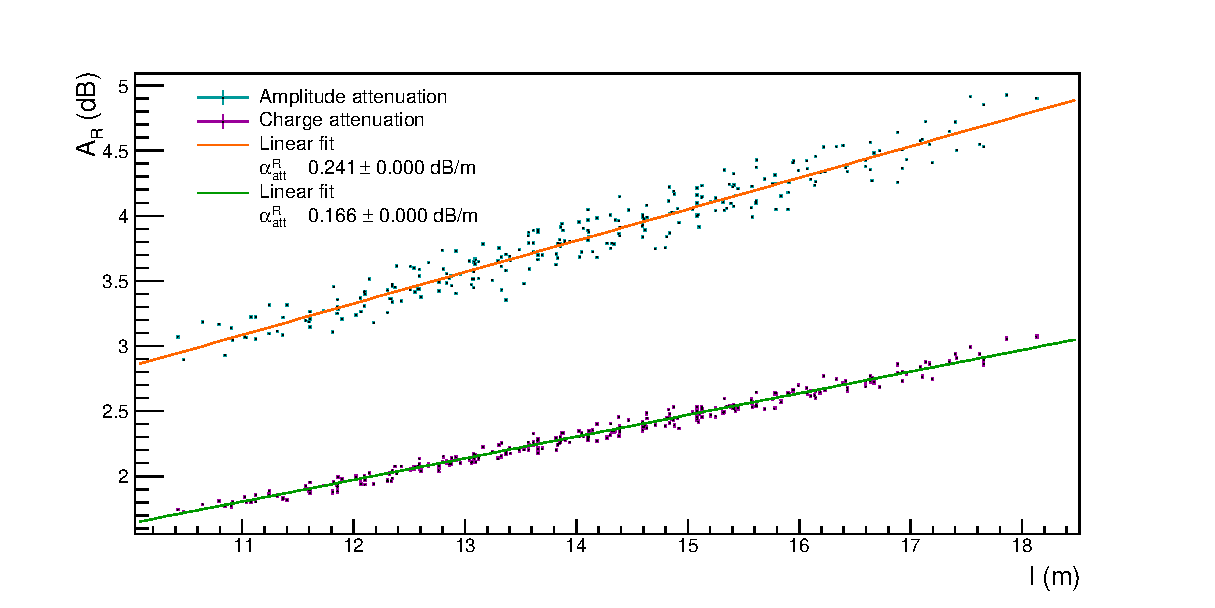
\includegraphics[width=15cm]{commissioning/fig_commissioning/attenuation_length.eps}
  \caption{The amplitude $\mathcal{A}$ is displayed as a function of the measured cable length $l$.
    The data set calculated with the amplitude (charge) is given in cyan (magenta) and fitted by a linear function in orange (green).
    The values of the slope, which represent the linear attenuation of the coaxial cables in dB/m, are respectively $\alpha_{\text{att}}^{\text{R, amp}} = 0.241\pm 0.000$dB/m and $\alpha_{\text{att}}^{\text{R, ch}} = 0.166\pm0.000$dB/m.
    The two $y$-intercept values, which represent the reflection of the pulse on the PMT divider, are $f_{r}^{amp} = 0.402\pm 0.032$ dB and $f_{r}^{ch} = -0.020\pm 0.013$ dB.
    \label{fig:attenuation}}
\end{figure}
The values of $\alpha_{\text{att}}^{\text{R}}$ and $f_{r}$, for both amplitude and charge cases, are displayed in the legend.
Firstly, the two linear fits reveal that, whether calculated with the amplitude, or with the charge, the linear attenuation $\alpha_{\text{att}}^{\text{R}}$ is smaller than the calculated one $\alpha_{\text{att}}^{\text{th}}$ (for the amplitude case, $\alpha_{\text{att}}^{\text{th}}\simeq 5\times \alpha_{\text{att}}^{\text{R, amp}}$, and for the charge case $\alpha_{\text{att}}^{\text{th}}\simeq 7\times \alpha_{\text{att}}^{\text{R, ch}}$).
That means the signal is less affected, when transmitted by the cable, than expected.
Secondly, the attenuation in charge is less important that the attenuation in amplitude.
This can be easily explained: as it is integrated over time, the charge is a quantity less affected by amplitude variations that the amplitude itself.
For the same reason, the charge data set points are less spread than the amplitude ones, meaning that we are less sensitive to cable length variations when using the charge quantity.


This work achieved, we want to verify if no cable was damaged after installation.
Reflectometry also aimed at checking cable conditions by performing waveform shape analysis on secondary pulses.

\subsection{Pulse shape analysis}
\label{subsec:pulse_shape}
In Fig.~\ref{fig:CFD} is displayed an example of \emph{normal} pulse, which corresponds to the case represented in Fig.~\ref{subfig:reflecto_normal}.
In this case, the pulse sent in the cable travels to the PMT, and goes back to the acquisition after reflection on the divider.


\subsection{Comparison with $^{60}$Co}

\subsection{Conclusion}
A faire : regarder le rising time en fonction de la longueur du cable\\
Regarder la différence de temps de montée du signal sur deux PMs très éloignés

\section{Calibrating the electronic boards}
\label{sec:TimeSynchroFEB}

\subsection{Principle}
\subsection{Measuring the time offset of front end boards}
\subsection{Results}


\section{Energy calibration of optical modules}
\label{sec:comm_energy_calibration}


*thèse Arnaud page 103*

As described in Sec.~\ref{subsec:OMtimeResponse}, the collected charge at PM voltage divider is proportional to the amount of incident photoelectrons, and then to the initially deposited energy inside the scintillator.
Once optical modules were assembled (optical coupling, packing, shielding integration), they were individually tested at Bordeaux laboratory, CENBG, with an electron spectrometer [ref].
Their energy resolutions for $1$ MeV-electrons at the centre of scintillator front face were determined.
High voltages were set to optimal values, to obtain an amplitude of $300$ mV for $1$ MeV electrons.
However, after calorimeter integration, due to different environment, amplitude spectra of each optical block have to be re-aligned.
This work was performed by Axel Pin, PhD student at CENBG.
We give in this section a summary of this energy calibration study.

*A finir\\




\section{Baseline studies}
\label{sec:comm_baseline}

\section{Light Injection System}
\label{sec:LI}

               \chapter{Characterisation of the calorimeter time resolution}
\label{ch:Cobalt_study}

The precise knowledge of the different particle interaction times in the optical modules of the SuperNEMO calorimeter is important to better understand and reject the background.
For example, the study of electron time-of-flight allows us to distinguish internal events (occurring within the source foils) from external events (radioactive decays occurring outside the source foils, for example in the PMTs or in the iron shielding).

During the commissioning phase, a lot of work, presented in the next chapter, was achieved to calibrate the detector.
Following on from this task and completing it, a great part of my PhD was allocated to determine the time resolution of the SuperNEMO calorimeter, and to provide tools to the collaboration to purchase this analysis.

In this chapter we present different studies conducted in order to characterise the time response of the SuperNEMO optical modules.
Although the goal of the presented studies is to characterise the time resolution of the SuperNEMO calorimeter, some detector adjustments were still ongoing at the time of the acquisition, that could influence the presented results.
Especially, the energy calibration described in Sec.~\ref{sec:comm_energy_calibration} was not complete, and the Light Injection System presented in Sec.~\ref{sec:LIS} was not yet fully operational.
However, all the work presented here is necessary in the framework of the first calorimeter calibration.
Moreover, I provide all the analysis tools for the collaboration, with a view to doing a possible update, once the whole demonstrator calibration will be achieved.

The first study presented in this chapter focuses on the characterisation of the time resolution of the SuperNEMO calorimeter, using a calibration source made of Cobalt $60$.
In the second part of this chapter, we study the possibility to gather informations on the calorimeter time resolution using the Light Injection System, a set-up initially designed to calibrate in energy the calorimeter.

%%%%%%%%%%%%%%%%%%%%%%%%%%%%%%%%%%%%%%%%%%%%%%%%%%%%%%%%%%%%%%%%%%%%%%%%%%%%%%%%%%%%%%%%%%%%%%%%%%%%%%%%%%%%%%%%%%%%%%%%%%%%%%%%
\section{Interaction of particles in the SuperNEMO scintillators}
\label{sec:scintillator_interactions}

Understanding how particles interact in the SuperNEMO scintillators is essential.
The calorimeter part of the demonstrator mainly aims to detect electrons and photons.
In this section, we review ***.


\subsection{Interaction of electrons}

Electrons interact with matter through one of two processes: elastic scattering on a nucleus, or inelastic scattering on an atomic electron.
Inelastic scatterings are dominant for polystyrene scintillators and occur through two different forms: coherent scattering with the electron cloud, and radiative energy losses (the so-called bremsstrahlung effect).
In Fig.~\ref{subfig:electron_attenuation} is displayed the stopping power of electrons in polystyrene for these two processes.
\begin{figure}[h]
  \centering
  \begin{subfigure}[t]{0.48\textwidth}
    \centering
    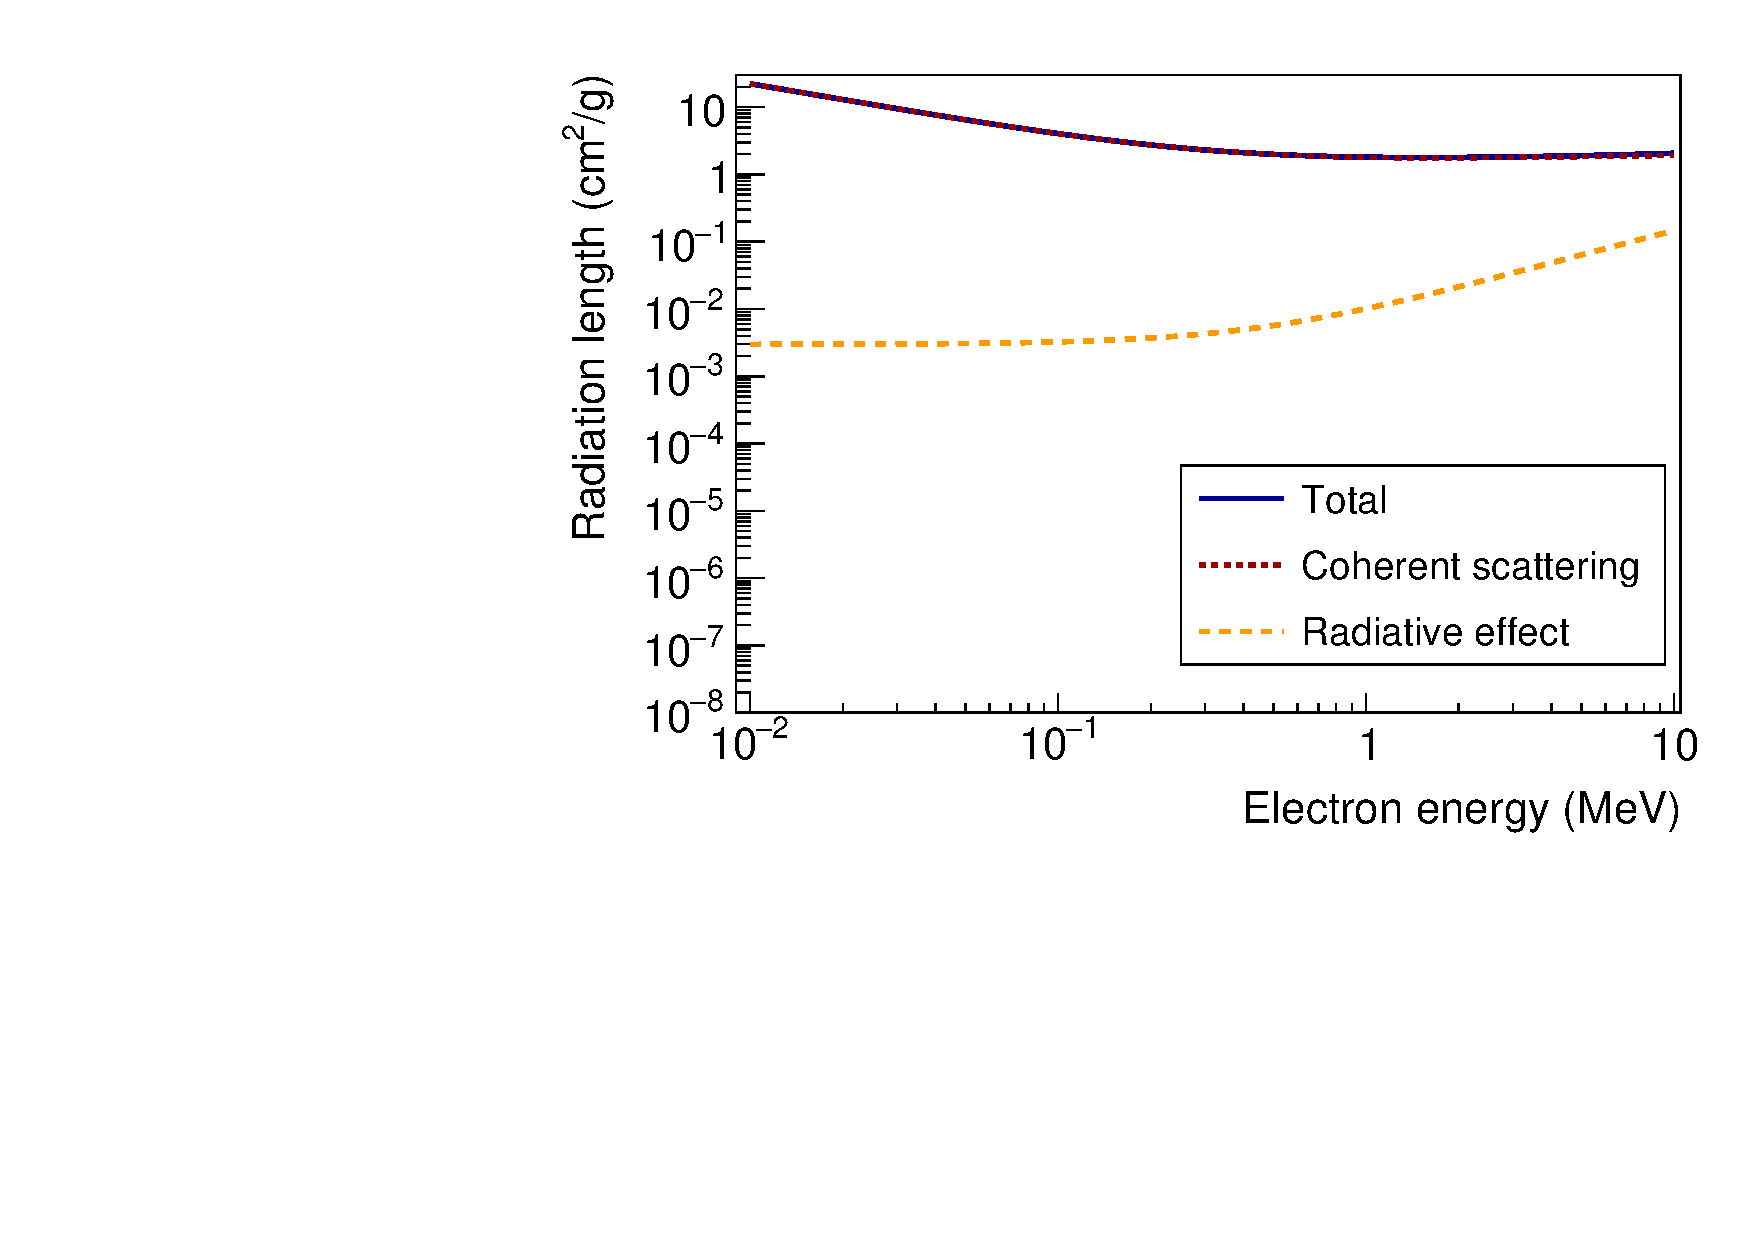
\includegraphics[width=1\textwidth]{commissioning/fig_commissioning/electron_energy_loss.pdf}
    \captionsetup{justification=centering}
    \caption{
      \label{subfig:electron_attenuation}}
  \end{subfigure}
  \hfill
  \begin{subfigure}[t]{0.48\textwidth}
    \centering
    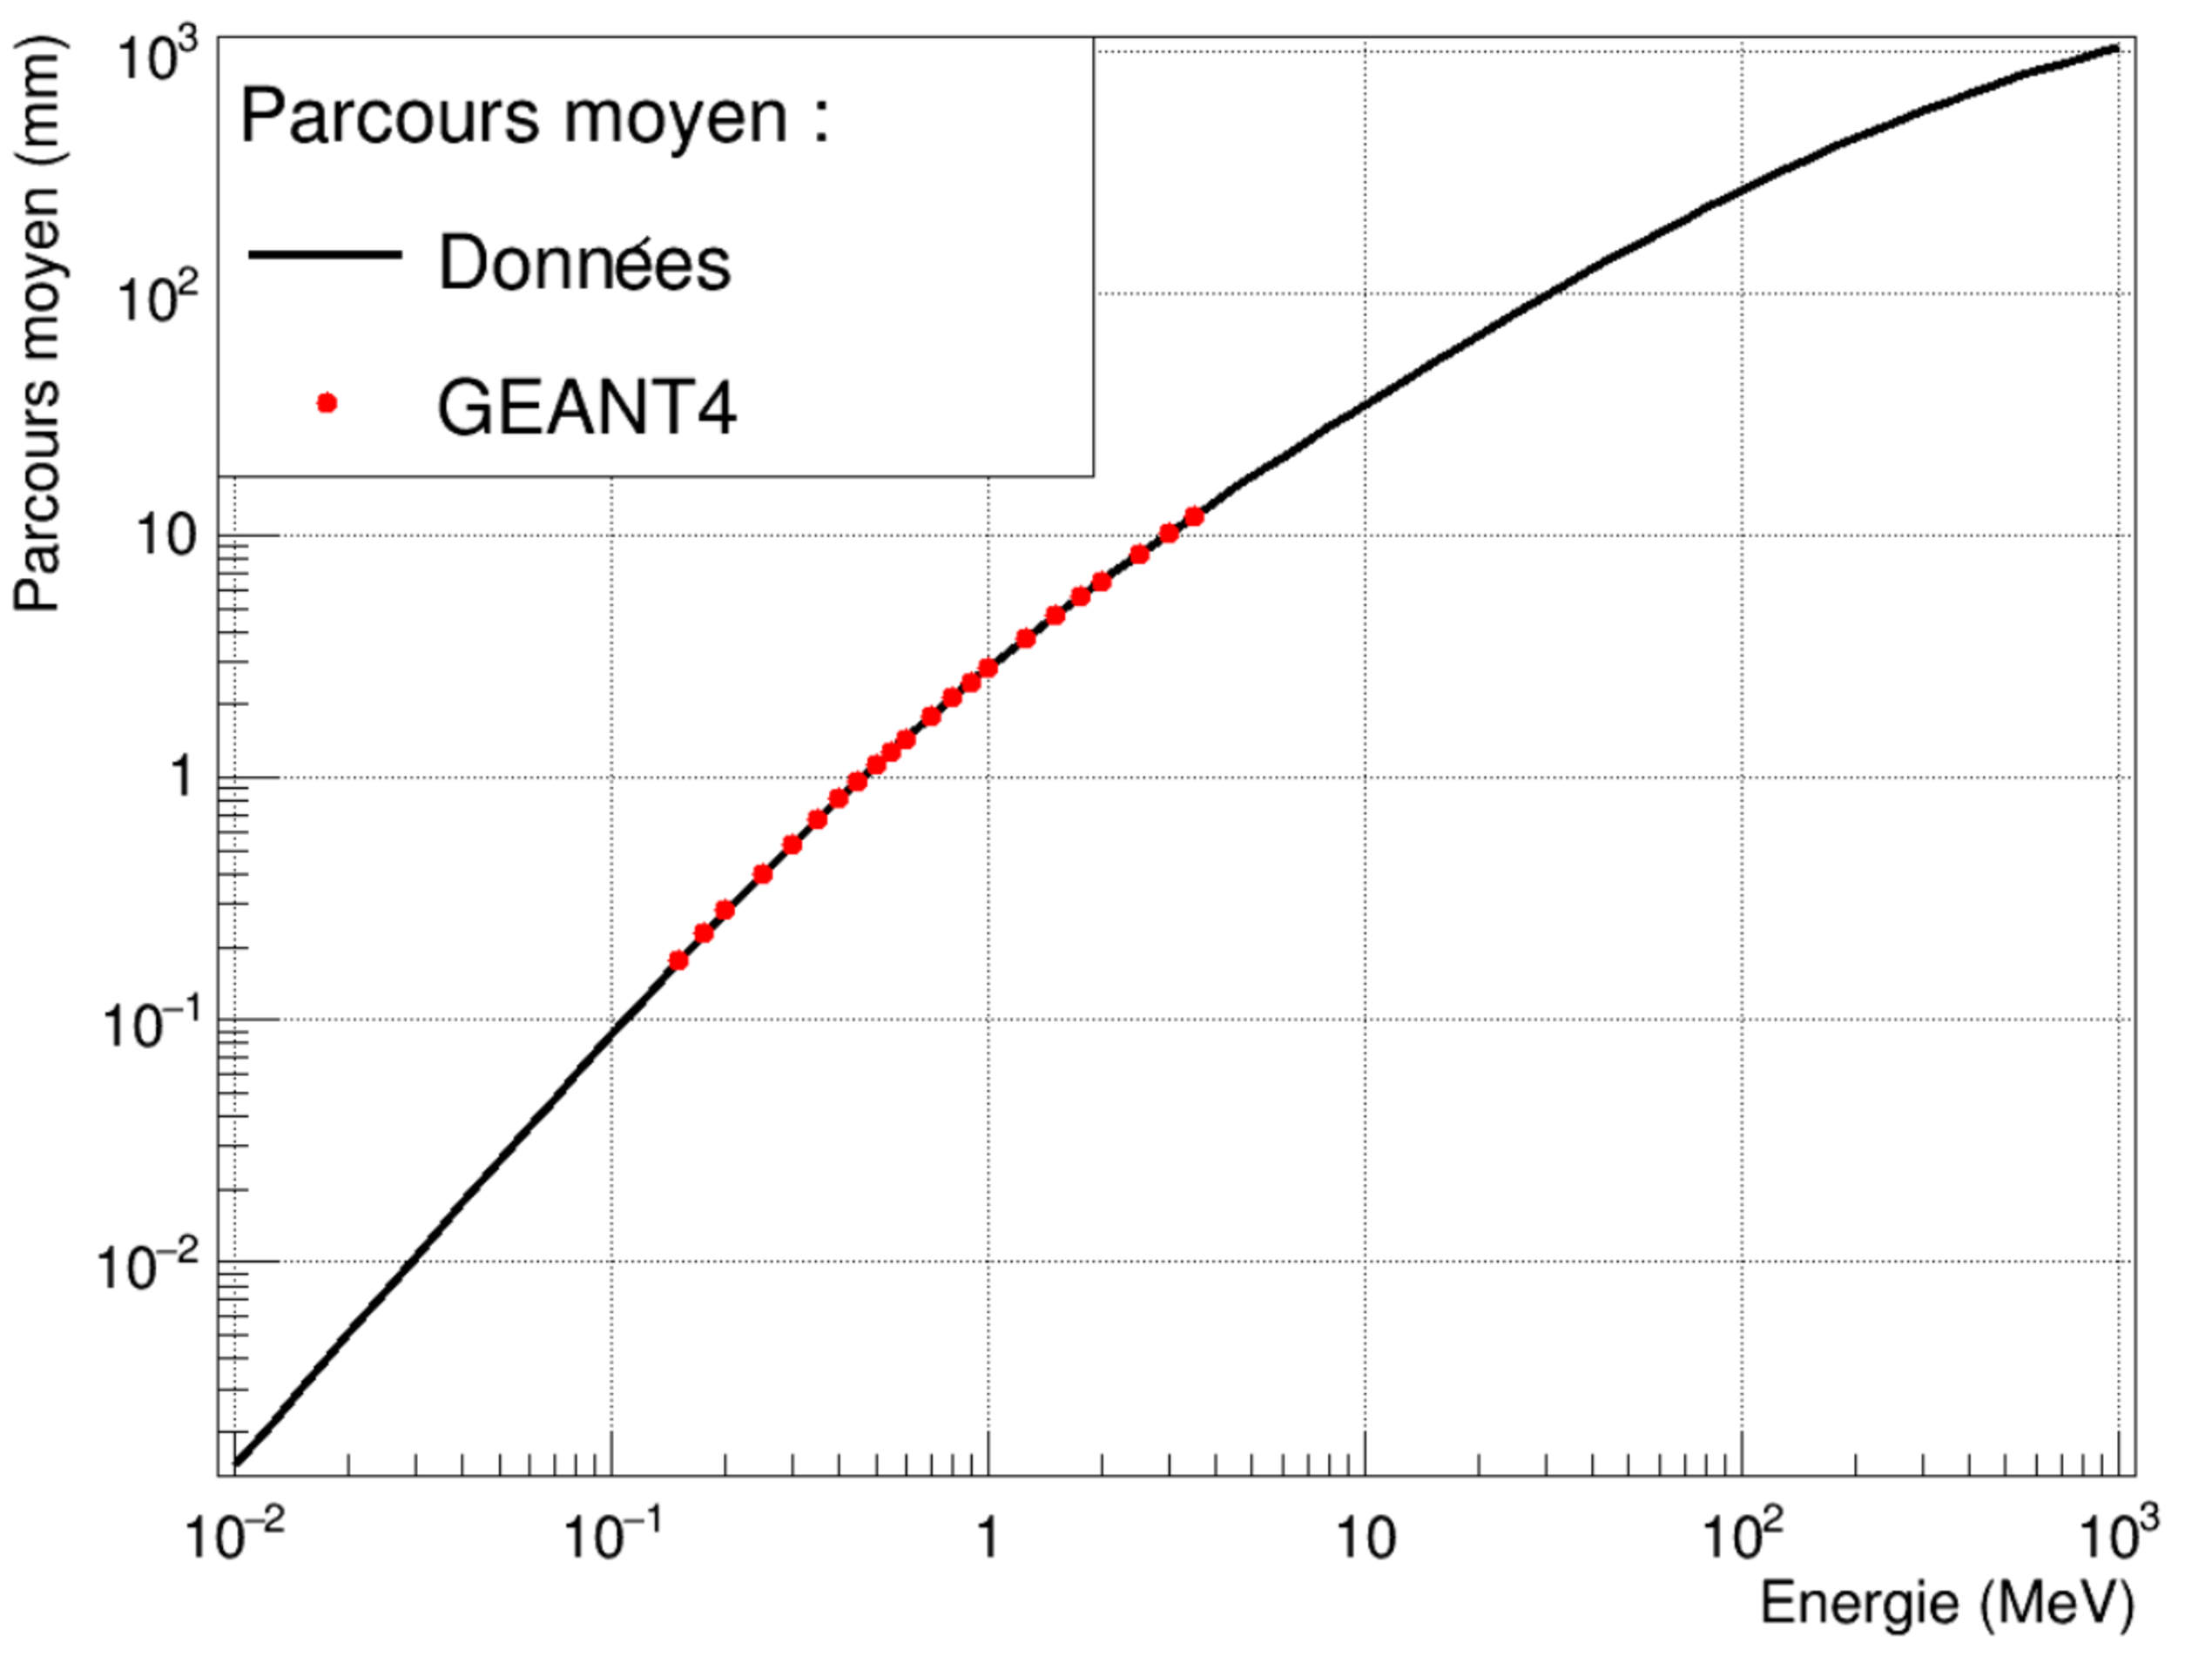
\includegraphics[width=1\textwidth]{commissioning/fig_commissioning/free_path_electrons.pdf}
    \captionsetup{justification=centering}
    \caption{\label{subfig:electron_free_path}}
  \end{subfigure}
  \caption{Stopping power (a) and mean free path (b) for electrons in polystyrene.
    (a) Energy losses through radiative effect (orange dashed line) and coherent scattering (red dashed line), which is the dominant process for the considered energy range~\cite{web:nist_estar}.
    %  operate mainly through coherent scattering.
    (b) At $1$ MeV, the mean free path of an electron is about $3$ mm.
    Adapted from~\cite{HuberThesis}.
  }
\end{figure}
Electrons detected in the SuperNEMO calorimeter should deposit a minimal energy of $50$ keV (the acquisition low energy threshold) and a maximal energy of few MeV (depending on the $\twonu$ isotope).
In this energy range, collisions with the electron cloud are preponderant compared with radiative energy losses.
In Fig.~\ref{subfig:electron_free_path}, we give informations about the mean free path of an electron in polystyrene.
In particular, we observe that an electron of $1$ MeV penetrates, in average, several millimetres into a polystyrene scintillator.


\subsection{Interaction of photons}

Photons travelling in  matter can interact with the electronic cloud, through three main processes, whose contributions are presented in fig.~\ref{subfig:photon_energy_loss}, depending on their energies.
\begin{figure}[h]
  \centering
  \begin{subfigure}[t]{0.48\textwidth}
    \centering
    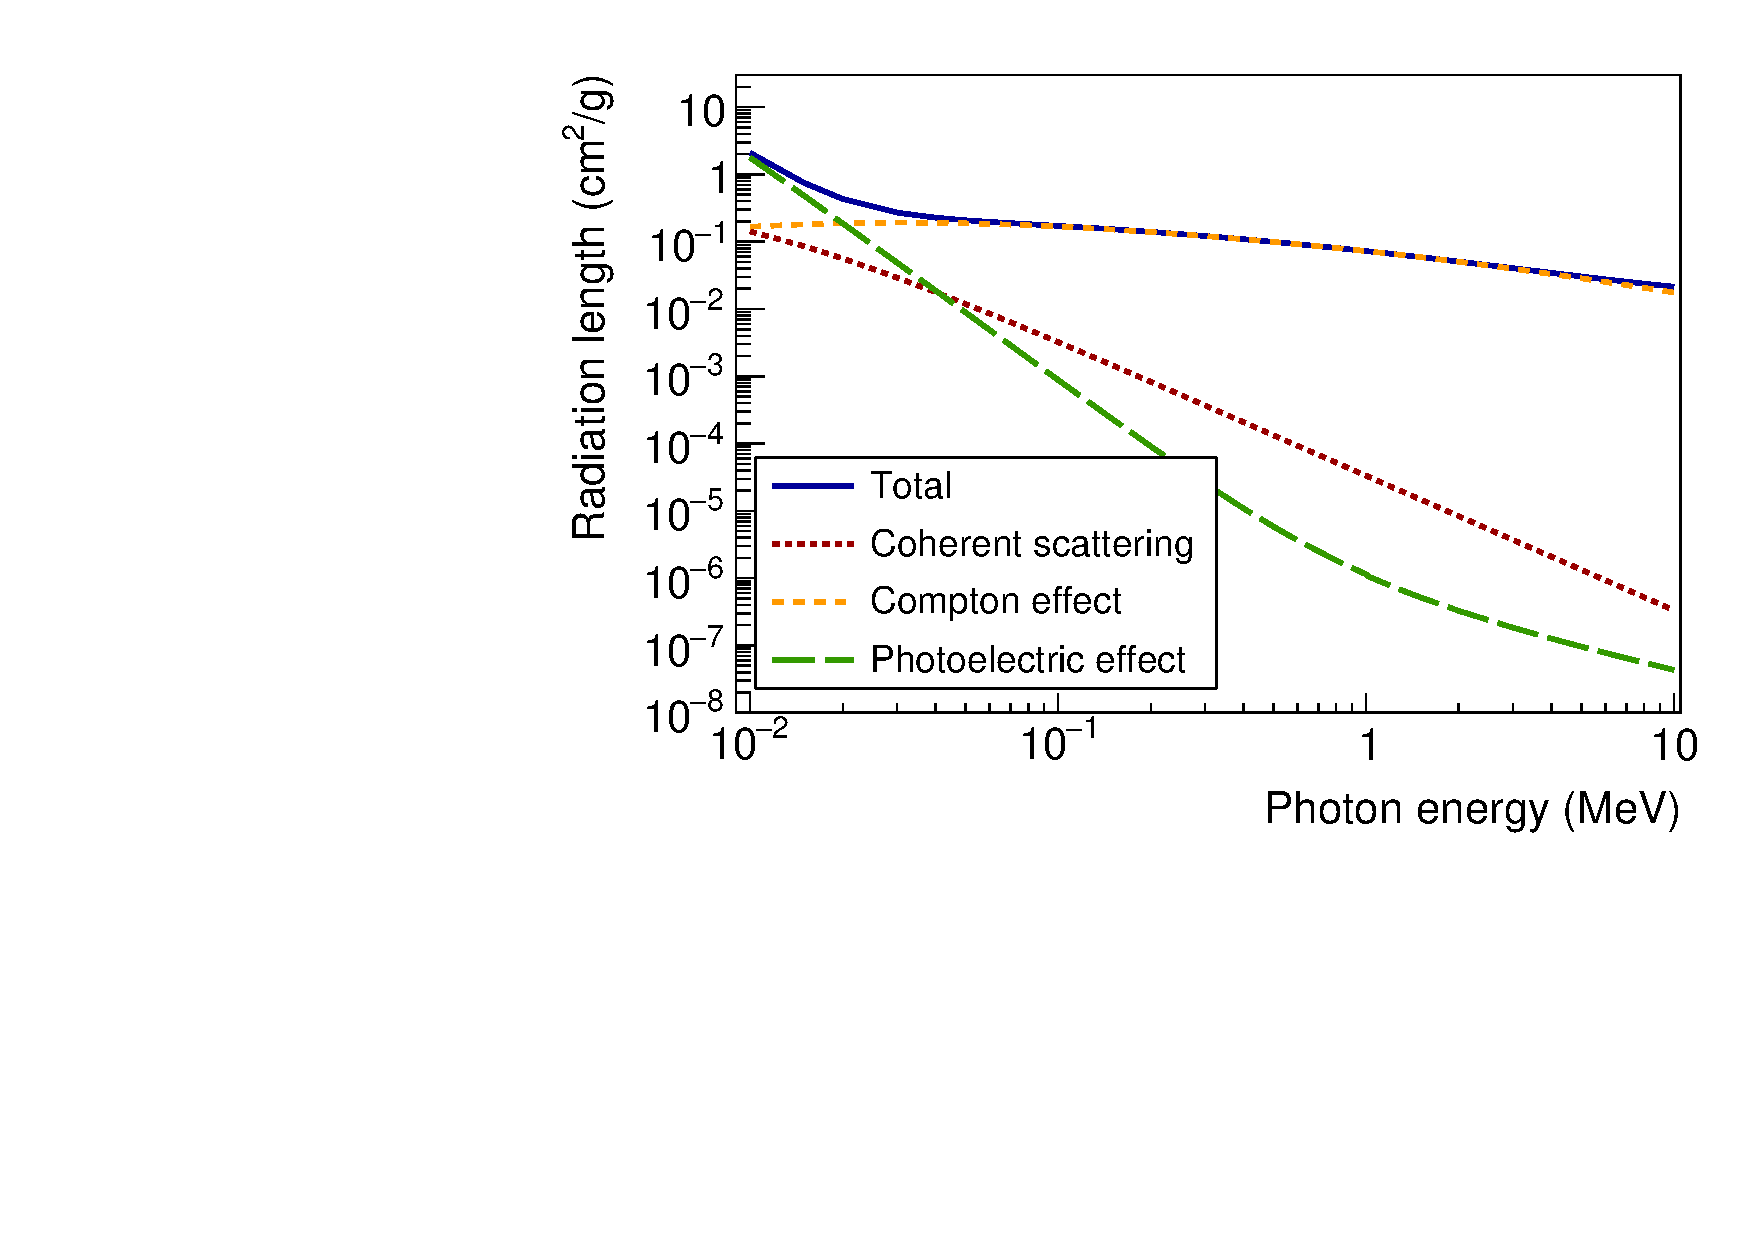
\includegraphics[width=1\textwidth]{commissioning/fig_commissioning/photon_energy_loss.pdf}
    \captionsetup{justification=centering}
    \caption{\label{subfig:photon_energy_loss}}
  \end{subfigure}
  \hfill
  \begin{subfigure}[t]{0.48\textwidth}
    \centering
    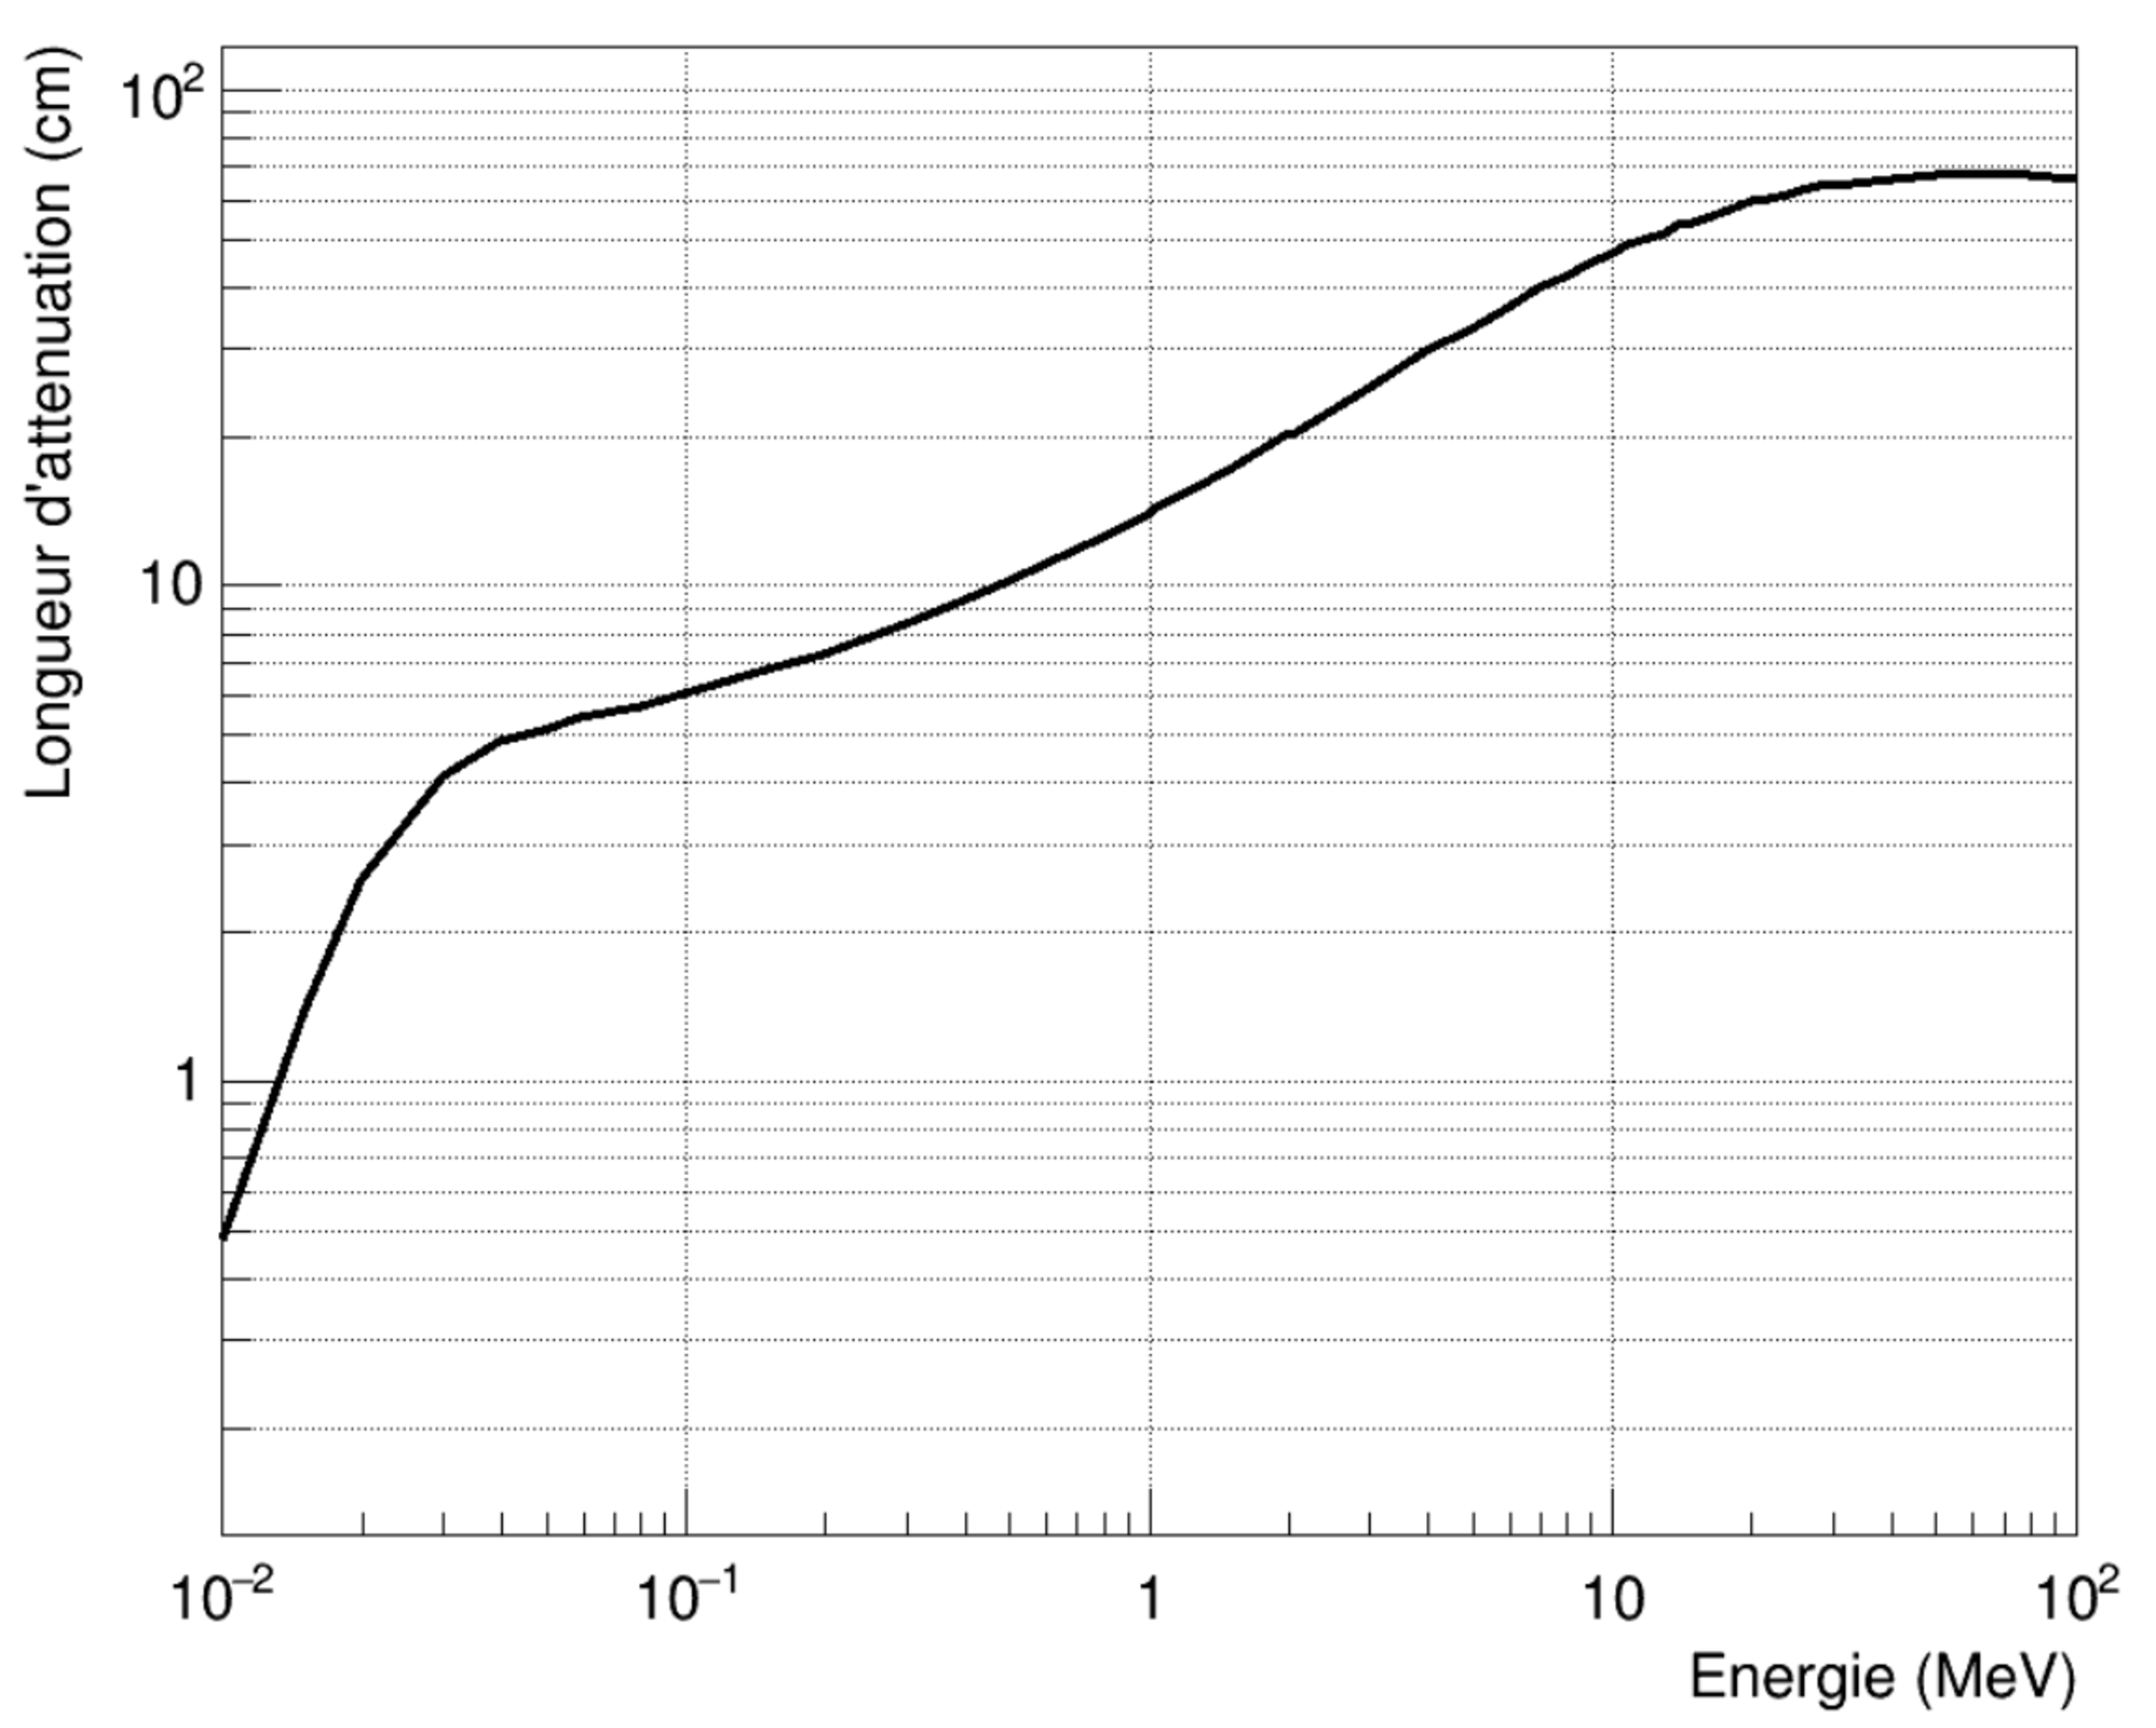
\includegraphics[width=1\textwidth]{commissioning/fig_commissioning/attenuation_length_photons.pdf}
    \captionsetup{justification=centering}
    \caption{\label{subfig:attenuation_length_photons}}
  \end{subfigure}
  \caption{Linear attenuation coefficient (a) and attenuation length (b) for $\gamma$ radiations in a plastic scintillator made of polystyrene.
    (a) In the considered energy range of $10$ keV $ -\; 10$ MeV, $\gamma$ radiations interact with matter mainly through Compton diffusion~\cite{web:nist_Xcom}.
    (b) The attenuation length of a $\gamma$ radiation is about $10$ cm at $1$ MeV.
    Adapted from~\cite{HuberThesis}.
  }
\end{figure}
Low-energy photons mainly interact with the electron cloud, either through photoelectric effect ($\gamma$ radiation is fully absorbed by an electron of the cloud), or through coherent (so-called Rayleigh) scattering.
But the dominant effect, for energies between $10$ keV and $10$ MeV, is the Compton inelastic scattering of a $\gamma$ with an atomic electron.
In Fig.~\ref{subfig:attenuation_length_photons}, we display the mean attenuation length of a $\gamma$ radiation in polystyrene scintillators, with energy.
Thus, most of $1$ MeV $\gamma$ radiations will interact around $10$ cm inside the scintillating material.

At the considered energy range ($10$ keV $ -\; 10$ MeV), the interaction of photons with matter is dominated by Compton effect, while the electrons interact mainly through coherent scattering.
The SuperNEMO scintillators are designed to detect such particles.
Photons have a high probability to interact inside the volume of the scintillator, while electrons are stopped in the first few millimetres.

The following section are devoted to the study of the time resolution of the SuperNEMO optical modules.



%%%%%%%%%%%%%%%%%%%%%%%%%%%%%%%%%%%%%%%%%%%%%%%%%%%%%%%%%%%%%%%%%%%%%%%%%%%%%%%%%%%%%%%%%%%%%%%%%%%%%%%%%%%%%%%%%%%%%%%%%%%%%%%%
\section{Measurement of the time resolution with a $^{60}$Co source}
\label{sec:Co_analysis}
This section is dedicated to detail the time resolution study performed using a Cobalt $60$ source, exploiting the time characteristic of two photons emitted during the radioactive disintegration process of this nucleus.
A great proportion of the whole SuperNEMO demonstrator was successfully characterised using this radioactive source.

\subsection{Description of Cobalt $60$ nucleus}
\label{subsec:CoSource}
The Cobalt $60$ is a man-made isotope, with a $5.27$ years half-life, of which we provide the main interesting properties in the simplified decay scheme of Fig.~\ref{fig:Co_decay_scheme}.
\begin{figure}[h]
  \centering
  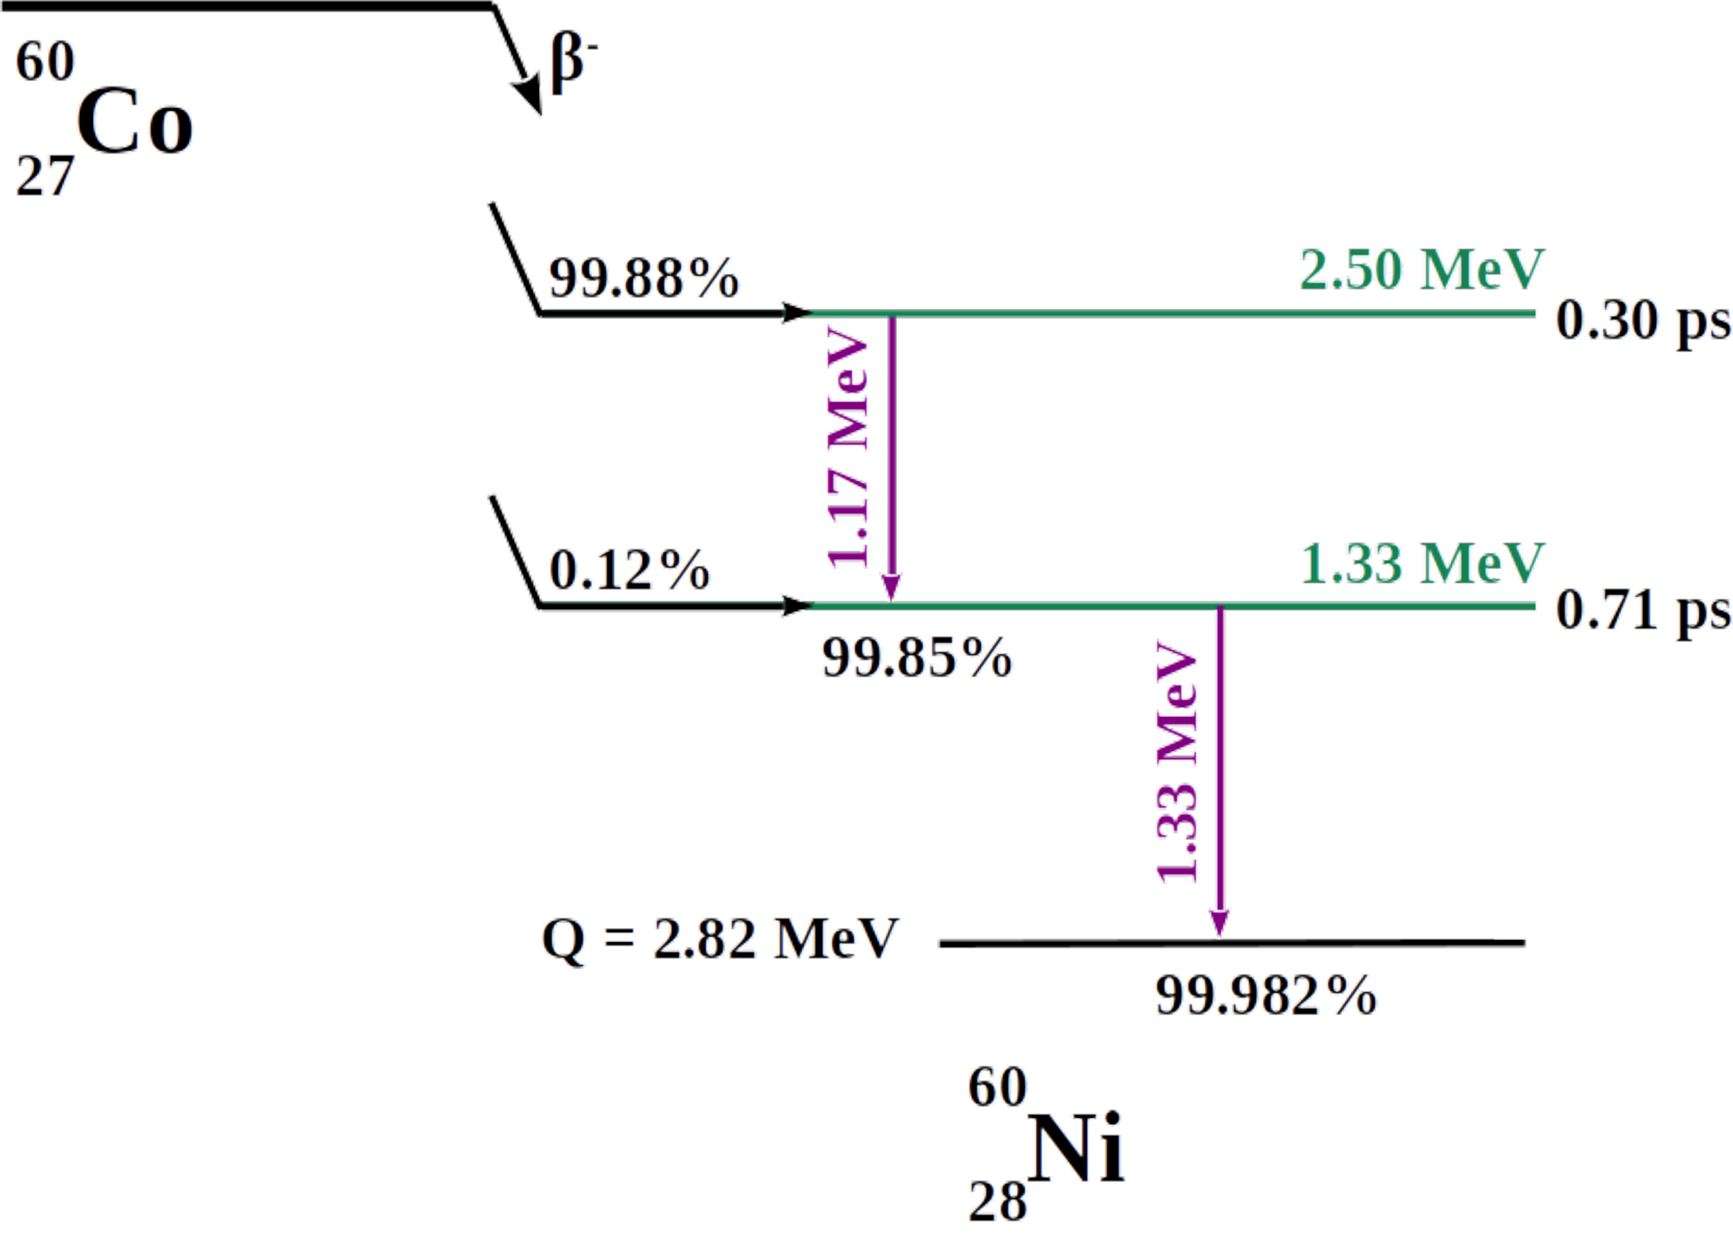
\includegraphics[width=9cm]{commissioning/fig_commissioning/Co_decay_scheme.pdf}
  \caption{A simplified decay scheme for Cobalt $60$ \cite{web:nucleide}.
    The Cobalt decays, through $\beta^{-}$, predominantly to the $2.50$ MeV state.
    Then, two succesive $\gamma$'s (whose energy levels are represented in green) are emitted in $99.83$\% of the cases.
    The two photons have an energy of $1.17$ MeV and $1.33$ MeV, respectively.
    As the life-time of the $1.33$ MeV energy level is short ($<1$ ps) with respect to the timing precision of the calorimeter, the two photons can be considered as emitted in coincidence.
    We use this property to calibrate in time the demonstrator optical modules.
    \label{fig:Co_decay_scheme}}
\end{figure}
This unstable nucleus spontaneously decays, through the $\beta^{-}$ process, into an excited state of Nickel $60$.
To reach the ground state of the Nickel $60$, the nucleus goes through two successive energy levels, emitting in $99.83$\% of the cases two photons of $1.17$ MeV and $1.33$ MeV, respectively.
The life-time of the second energy level is under the picosecond, thus very short with respect to the expected timing precision of the calorimeter.
Therefore, the two photons are considered as emitted in coincidence.

We aim to exploit these two photons emitted after the $\beta^{-}$ disintegration to determine the calorimeter time resolution.

\subsection{Time response of optical modules}
\label{subsec:OMtimeResponse}

In order to characterise the energy and time-of-flight of incoming particles (photons, electrons), each calorimeter block of SuperNEMO is composed of a scintillator and a photomultiplier.
As detailed in Chapter~\ref{ch:detector}, the purpose of the scintillator material is to stop the incoming particles, which will induce the production of the so-called optical photons.
The optical photons reaching the photomultiplier photocathode are then converted into electrons, with an efficiency called quantum efficiency.
After amplification, electrons are collected by the anode which delivers an electric signal whose charge proportional to the initial amount of incident photoelectrons.
This signal is then transmitted, via the PM voltage divider, to the electronic readout, where the signal is sampled.
The particle energy, as well as the time-of-flight, can be extracted from the signal waveform analysis.
Each step of the particle detection process, from the incident particle interaction inside the scintillator, to the signal sampling at the electronic readout, can have an impact on the precise time measurement of the charged particle.
In Chapter~\ref{ch:detector} and \ref{ch:timediff} we introduced the so-called calorimeter time resolution $\sigma_t$, which encapsulates the global uncertainty on the time-of-flight measurement of particles into the calorimeter (Eq.~\eqref{eq:sigma_t}).
The squared time-resolution can therefore be expressed as the sum of two contributions:
the scintillator resolution $\sigma_{t, \textrm{sc}}^{2}$, and the PMT resolution $\sigma_{t, \textrm{PM}}^{2}$,
\begin{equation}
  \sigma_{t}^{2}=\sigma_{t,\text{sc}}^{2}+\sigma_{t,\text{PM}}^{2}\,.
  \label{eq:Co_sigma_t}
\end{equation}
In the following, we detail in depth the physical origins of these terms.

\subsubsection*{Scintillator time dispersion}
The scintillator temporal dispersion $\sigma_{t,\text{sc}}$ in Eq.~\eqref{eq:Co_sigma_t} receives contributions mainly from two important characteristics of the scintillator operating principle.

\paragraph{Interaction point:}
The incoming particle's interaction point location inside the scintillator block highly contributes to the scintillator temporal uncertainty, and depends on the incident particle type.
In fact, this effect will not have the same impact on time dispersion, depending on whether the incident particle is a photon or an electron.
In Fig~\ref{fig:photon_scintilator} are schemed the interactions of a photon and that of an electron for the specific case of a SuperNEMO plastic scintillator.
\begin{figure}[h]
  \centering
  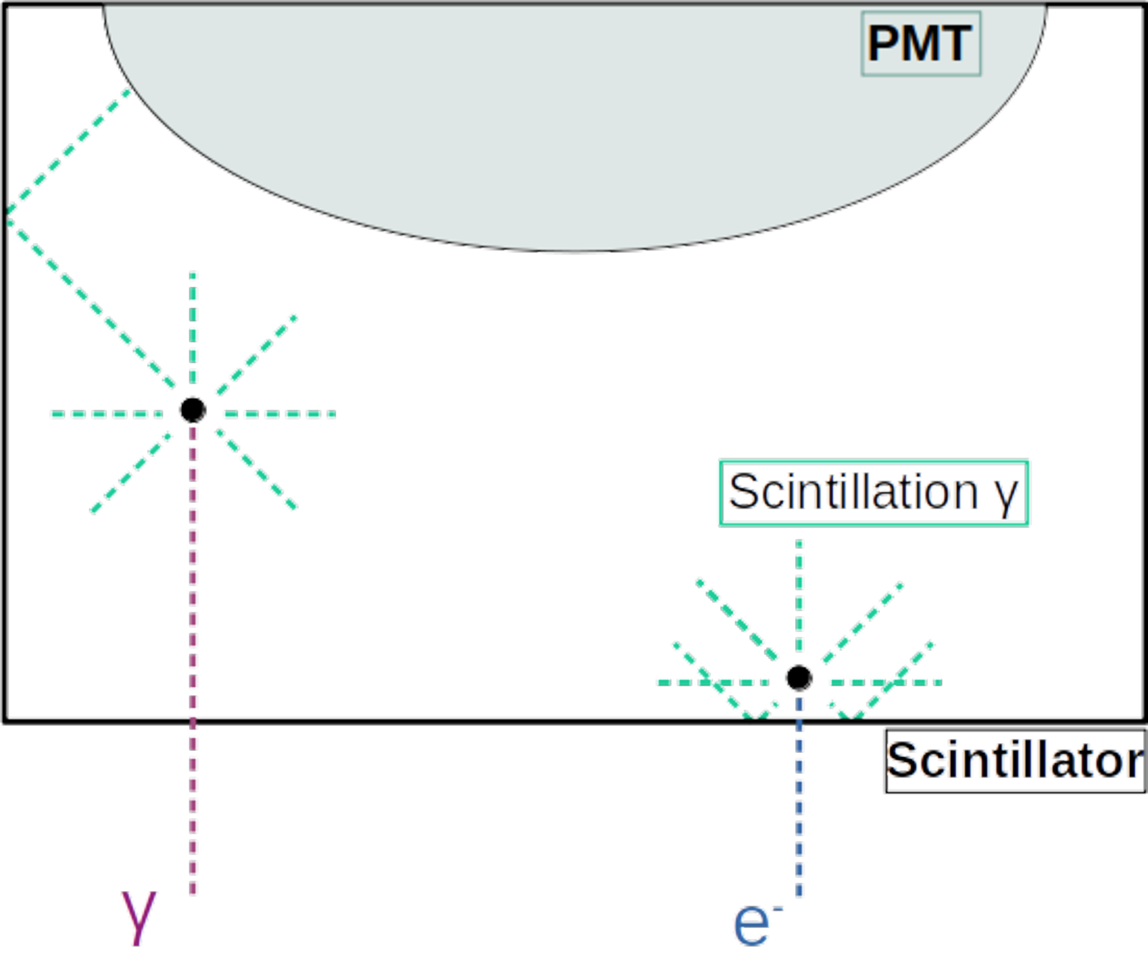
\includegraphics[width=8cm]{commissioning/fig_commissioning/Co_multi_reflection.pdf}
  \caption{A scheme of interaction of particles in a scintillator.
    The photon case is displayed on the left in pink dotted line, and the electron case is on the right in dark blue dotted line.
    Both particles enter in the scintillator through the front face.
    Examples of interaction points inside the scintillator are represented by the black dots.
    The photons of scintillation emitted isotropically after the interaction are materialised by the bright green dotted lines.
    Due to different interaction probabilities in matter, the two particles intercat at different depths inside the scintillator.
    The photon can interact deeply inside the volume, while the electron has a high probability to stop within the first few millimetres.
    \label{fig:photon_scintilator}}
\end{figure}
In Sec.~\ref{sec:scintillator_interactions}, we exposed the different interaction types of photons and electrons.
We have also explained the origin of the differences that exist in terms of interaction depth between these two types of particles.
To remain consistent with these conclusions, we represent the electron as interacting in the first millimetres, while the photon stops deep inside the scintillator.
When a particle (photon or electron) interacts in the scintillating material, the absorbed energy leads to the isotropic emission of scintillation photons:
they propagate inside the scintillator, in all directions from the interaction point, at the speed of $c/n_{sc}$, with $n_{sc}$ the optical index of polystyrene, and $c$ the light speed in vacuum.
Depending on their initial direction, some of those photons propagate straight to the PMT (we name them the \emph{direct} photons), while others are at least reflected once on the scintillator surface, before reaching the PM glass.
This mechanism leads to time delays between direct and reflected photons.

In order to illustrate, and give an order of magnitude of this delay, let us consider an example where an incoming electromagnetic particle enters a scintillator from the front face, and interacts right in the centre of the scintillator volume.
After the scintillation emission process, a direct photon will reach the PM glass surface at time
\begin{equation}
  t_{s} = \frac{L}{2c/n_{sc}}\,,
\end{equation}
$L$ being the scintillator width.
Now, let us consider another photon, that we name \emph{backward reflected}, emitted in the opposite direction.
It will propagate, reflect on the front scintillator surface, and finally reach the PM at
\begin{equation}
  t_{r} = \frac{3L}{2c/n_{sc}}\,.
\end{equation}
This reflected photon is therefore delayed compared to the direct photon, with a time-shift of
\begin{equation}
  \Delta t^{r,s} = t_{r} - t_{s} = \frac{L}{c/n_{sc}}\,.
\end{equation}
In the case of a SuperNEMO scintillator, the length $L$ has been designed to $25$ cm, and the optical index is the one of polystyrene with $n_{sc}=1.5$.
Finally, for an incoming particle interacting at the centre of a SuperNEMO scintillator volume, a backward reflected scintillation photon will reach the PM glass $1.25$ ns later than a direct photon.
And this delay is even more important as the incident particle interacts deep inside the scintillator.

In view of the conclusions given in Sec.~\ref{sec:scintillator_interactions}, we know that photons have a higher probability of interacting far into the scintillator block, compared with electrons.
Therefore, this time-shift effect is all the more important for incoming photons, while it is quite negligible for incoming electrons, for which reflected photoelectrons reach the PM glass almost as the same time as the direct ones.

This mechanism increases the signal collection rising time at the PM anode, and boosts the scintillator time dispersion $\sigma_{t,\text{sc}}$, with $\sigma_{t,\text{sc}}^{\gamma}>\sigma_{t,\text{sc}}^{\text{e}^{-}}$.

\paragraph{Scintillating light emission:}
When a particle interacts in a SuperNEMO scintillator, two successive mechanisms of light absorption/re-emission take place.
Firstly, the excitation of scintillator molecules leads to the creation of fluorescence photons.
Afterwards, those optical photons are absorbed, then re-emitted by the POPOP agent, at higher wavelengths.
The characteristic times of these two processes contribute to increase the scintillator time dispersion $\sigma_{t,\text{sc}}$.
%% These two processes follow the same temporal distribution
%% \begin{equation}
%%   \mathcal{N}_{\text{photons}} = A\times e^{-t/\tau}\,,
%%   \label{eq:fluorescence_photons_time}
%% \end{equation}
%% with $\mathcal{N}_{\text{photons}}$ the number of generated photons at time $t$, $A$ a normalisation constant and $\tau$ the fluorescence characteristic time of the considered process.

Now that two main contributions accounting for the uncertainty on time measurement taken by the scintillator had been developed, we detail the origin of the second term of Eq.~\eqref{eq:Co_sigma_t}, $\sigma_{t,\text{PM}}$.

\subsubsection*{Photomultiplier time dispersion}

A photomultiplier is a photodetector: after the light is collected and converted at the photocathode, the photoelectrons are multiplied.
The transit time for the photoelectrons emitted at the photocathode to reach the anode after being multiplied is not constant for every photoelectron, due to a varying path for electrons emitted by the different dynodes.
This results in a timing dispersion.
This fluctuation is called transit time spread (TTS).
It leads to an uncertainty on the time measurement and so has an influence on the photomultiplier time dispersion $\sigma_{t,\text{PM}}$.

In the following, we describe how we characterised the time dispersion brought by the optical module on the time measurement, using a Cobalt 60 source.


\subsection{Experimental design}
\label{subsec:Co_setup}


The idea to use a Cobalt $60$ source to characterise the time response of the calorimeter part of SuperNEMO had never been tested before the current analysis.
Therefore, all the experimental design had to be implemented.


\subsubsection*{Setting up the experimental design}


The initial activity of the Cobalt source we used for this experimental set-up was $447.4$ kBq in February $2014$.
Given the half-life of this isotope, it was reduced to $232$ kBq at the time of the data-taking.
In order to determine the best design, and later to monitor and compare the results obtained in the framework of this analysis, I performed simulations of \Co\ disintegrations for the demonstrator configuration.
The characteristics of those simulations are detailed later in this section.

As described in Chapter~\ref{ch:detector}, the SuperNEMO calorimeter is composed of two main walls (called \emph{French} and \emph{Italian} sides), as well as the so-called X-Walls (on the detector sides) and $\gamma$-Vetos (on top and below the detector).
At the time of the data-taking, X-Walls and $\gamma$-Vetos were not yet operational, hence the current analysis only applies on the French and Italian main calorimeter walls.
As the demonstrator was closed at this time, it was impossible to set the Cobalt source inside the detector, at the source foils level.
Hence, the calibration source was placed behind the calorimeter, as displayed in Fig.~\ref{fig:Co_exp_design}, where sketches of side and back views of the calorimeter are drawn.
\begin{figure}[h]
  \centering
  \begin{subfigure}[t]{0.48\textwidth}
    \centering
    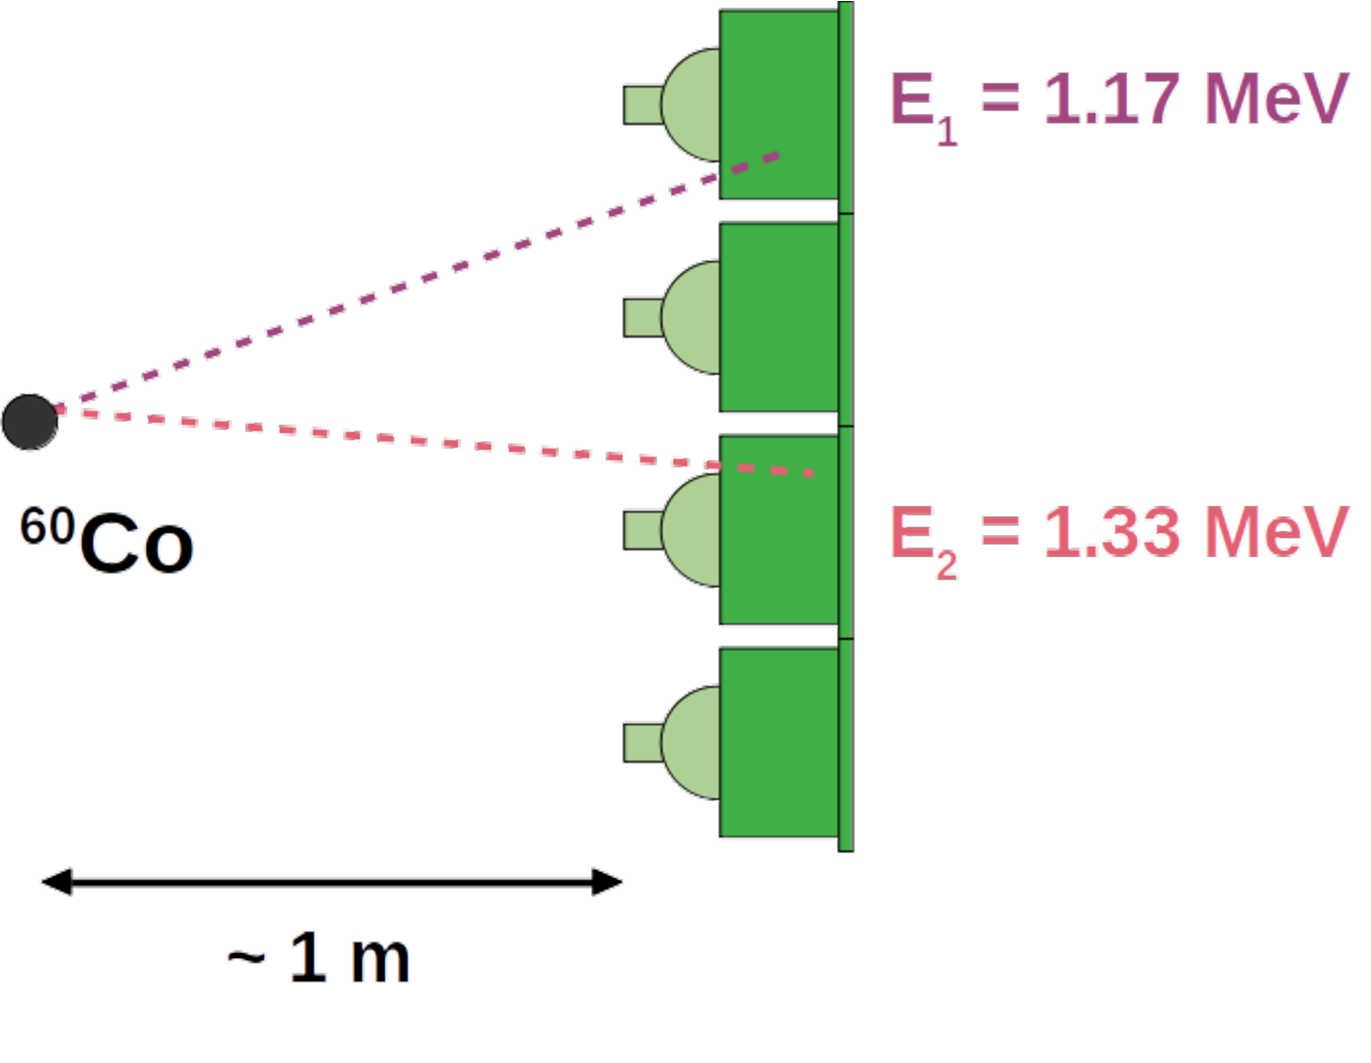
\includegraphics[height=0.5\textwidth]{commissioning/fig_commissioning/Co_setup.pdf}
    \captionsetup{justification=justified}
    \caption{
      \label{subfig:Co_setup}}
  \end{subfigure}
  \hfill
  \begin{subfigure}[t]{0.48\textwidth}
    \centering
    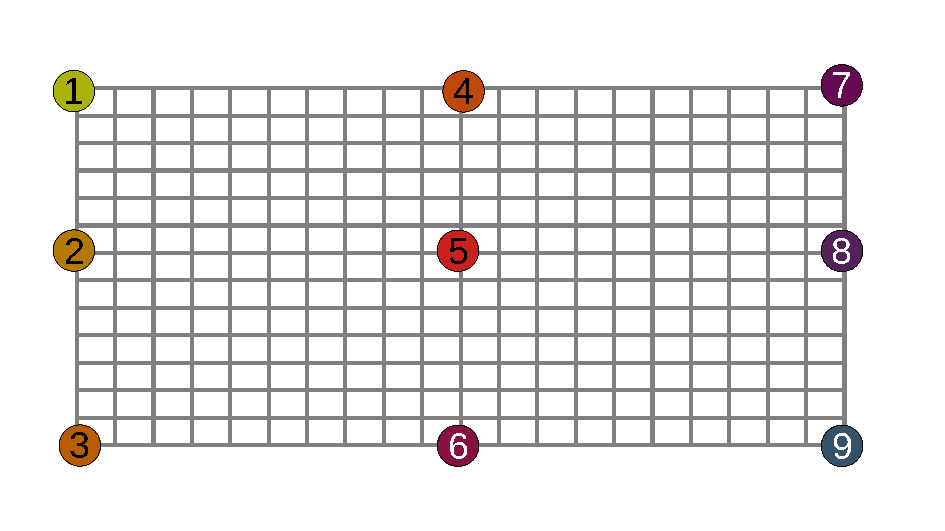
\includegraphics[height=0.5\textwidth]{commissioning/fig_commissioning/Co_setup_wall.pdf}
    \captionsetup{justification=justified}
    \caption{
      \label{subfig:Co_setup_wall}}
  \end{subfigure}
  \caption{(a) Side view example of the Cobalt source positioning behind a calorimeter main wall, schemed by $4$ optical modules (green).
    The emissions of the $2$ $\gamma$'s of interest are displayed in coloured dotted lines.
    (b) Back view of the nine source positions behind a main wall.
    Each grey box represents an optical module.
    \label{fig:Co_exp_design}
  }
\end{figure}
In order for all PMs to detect $\gamma$'s from Cobalt decays, several bunches of data acquisitions were taken:
the source was placed at $9$ different positions on each of the $2$ main calorimeter walls, approximately one meter behind.
Therefore, in total, $19$ data acquisitions have been taken, of which:
\begin{itemize}
\item $18$ with the Cobalt source set behind the wall. The $9$ different positions for one wall are represented in Fig.~\ref{subfig:Co_setup_wall}.
\item $1$ acquisition have been taken without the Cobalt source, with the Italian main wall, to characterise the background detected with the current calorimeter settings.
\end{itemize}
Each data acquisition lasted about $25$ minutes, for a total of $10$ hours of on-site activities, taking into account the time needed to move the Cobalt source from spot to spot.

Currently, the demonstrator is not protected from the laboratory lights by the anti-radon tent.
As laboratory lights would damage the SuperNEMO photomultipliers under tension, two removable black curtains are deployed on top of the detector (that do not interfere with data collection), and acquisitions are taken in dark laboratory.
With this way of doing, all data acquisitions can be performed, while eventual necessary repairs remain possible during the detector commissioning.

Taking acquisitions in the dark is a big constraint.
Moreover, the Cobalt source, initially used for teaching purposes, was loan by IPN laboratory (Orsay), for only two weeks, mainly because of legal constraints.
Therefore, to not disturb LSM on-site activities by plunging the whole laboratory into darkness, and to make the loan time profitable, a SuperNEMO team and I performed night shifts to take data.
The acquisition took place during two weeks, at the summer break $2019$.

\subsubsection*{Simulations and analysis pipelines}

The same way as for the Thallium study discussed in Chapter~\ref{ch:timediff}, all simulations were performed with an ideal calorimeter, setting up the uncertainty on optical modules to zero.
The same Root code was also used to adjust this parameter to the desired value.

As for the data acquisition, the simulated source has been placed behind the calorimeter walls.
Hopefully, there was no need to simulate all the $18$ positions.
In fact, at this time, the detector implemented in simulations is symmetrical in terms of detection performances.
Therefore, simulations of \Co\ events behind the two main walls are equivalent, and we only need to simulate events from $4$ locations (positions $1$, $2$, $4$ and $5$, according to the Fig.~\ref{subfig:Co_setup_wall} numbering system), other being obtained by symmetry operations.
Four bunches, for a total of $10^{9}$ Cobalt events, were simulated with the official Falaise pipeline and stored at the IN$2$P$3$ computing centre platform, making them available to the collaboration.
%% A visualisation, provided by the Falaise Software, of a simulated Cobalt event behind the Italian calorimeter main wall, is shown in Fig.~\ref{fig:Co_visu}.
%% \begin{figure}[h]
%%   \centering
%%   
\includegraphics[width=6cm]{commissioning/fig_commissioning/Co_visu.pdf}
%%   \caption{Visualisation of a simulated Cobalt event.
%%     \label{fig:Co_visu}}
%% \end{figure}

%% \paragraph{Background events simulations:}
%% As already discussed in Chapter~\ref{ch:sensitivity}, currently the collaboration does not supply a complete set of external background simulations for the demonstrator design.
%% This will be implemented as soon as the final demonstrator performances has been determined.
%% Thus, we did not have at our disposal background events simulations for this analysis.

The entire experimental set-up was designed and carried out by me and a group of physicists from LAL, Orsay and LPC, Caen.
I developed a complete set of ROOT codes for data processing and analysis, available on the GitHub platform~\cite{myGit}.
As the tracker is not yet operational for data collection at Modane, we are only interested in the part of the simulations with the calorimeter.
The PID module was therefore not used in the reconstruction pipeline, and other criteria, described in the following sub-section, were used to select the Cobalt events of interest.
A single off-line analysis pipeline has been developed to handle the different output data models of the simulations and real data, in order to ensure the consistency of the analysis.

\subsection{Signal events selection}
\label{subsec:Co_datacut}

We aim to use the two $\gamma$'s of $1.17$ MeV and $1.33$ MeV from Cobalt $60$ $\beta^{-}$ decay, to characterise the time resolutions of individual optical modules.
Thus, the signal we are looking for is two particles detected in coincidence in distinct optical modules.
In order to maximise the signal to background ratio, some selections have been applied on data.
\begin{itemize}
\item Trigger criteria:\\ in the two calorimeter hits channel, the trigger condition is defined so as one of the two hit has to trigger the low energy (or amplitude) threshold, of $50$~keV for the data acquisition.
  As we look for two calorimeter hits, we set an additional off-line selection events whose two hits passed both the high amplitude threshold, corresponding to approximately $150$ keV.
\item Coincidence time criterion:\\ we define the coincidence time-window by events occurring in a $62.5$ ns-long time interval.
  This allows to avoid accidental coincidence events (interactions of two gammas, produced by different sources, in two optical modules), while keeping events where two $\gamma$ particles interact at both ends of the wall.
  This time-window was set for the data-taking and can be improved for eventual future acquisitions.
\item Individual energy selection:\\ in Fig.~\ref{fig:Co_energy_cut} is displayed the hit of highest energy as a function of the one of lowest energy, for simulations with the \Co\ source in position $5$.
  \begin{figure}[h]
    \centering
    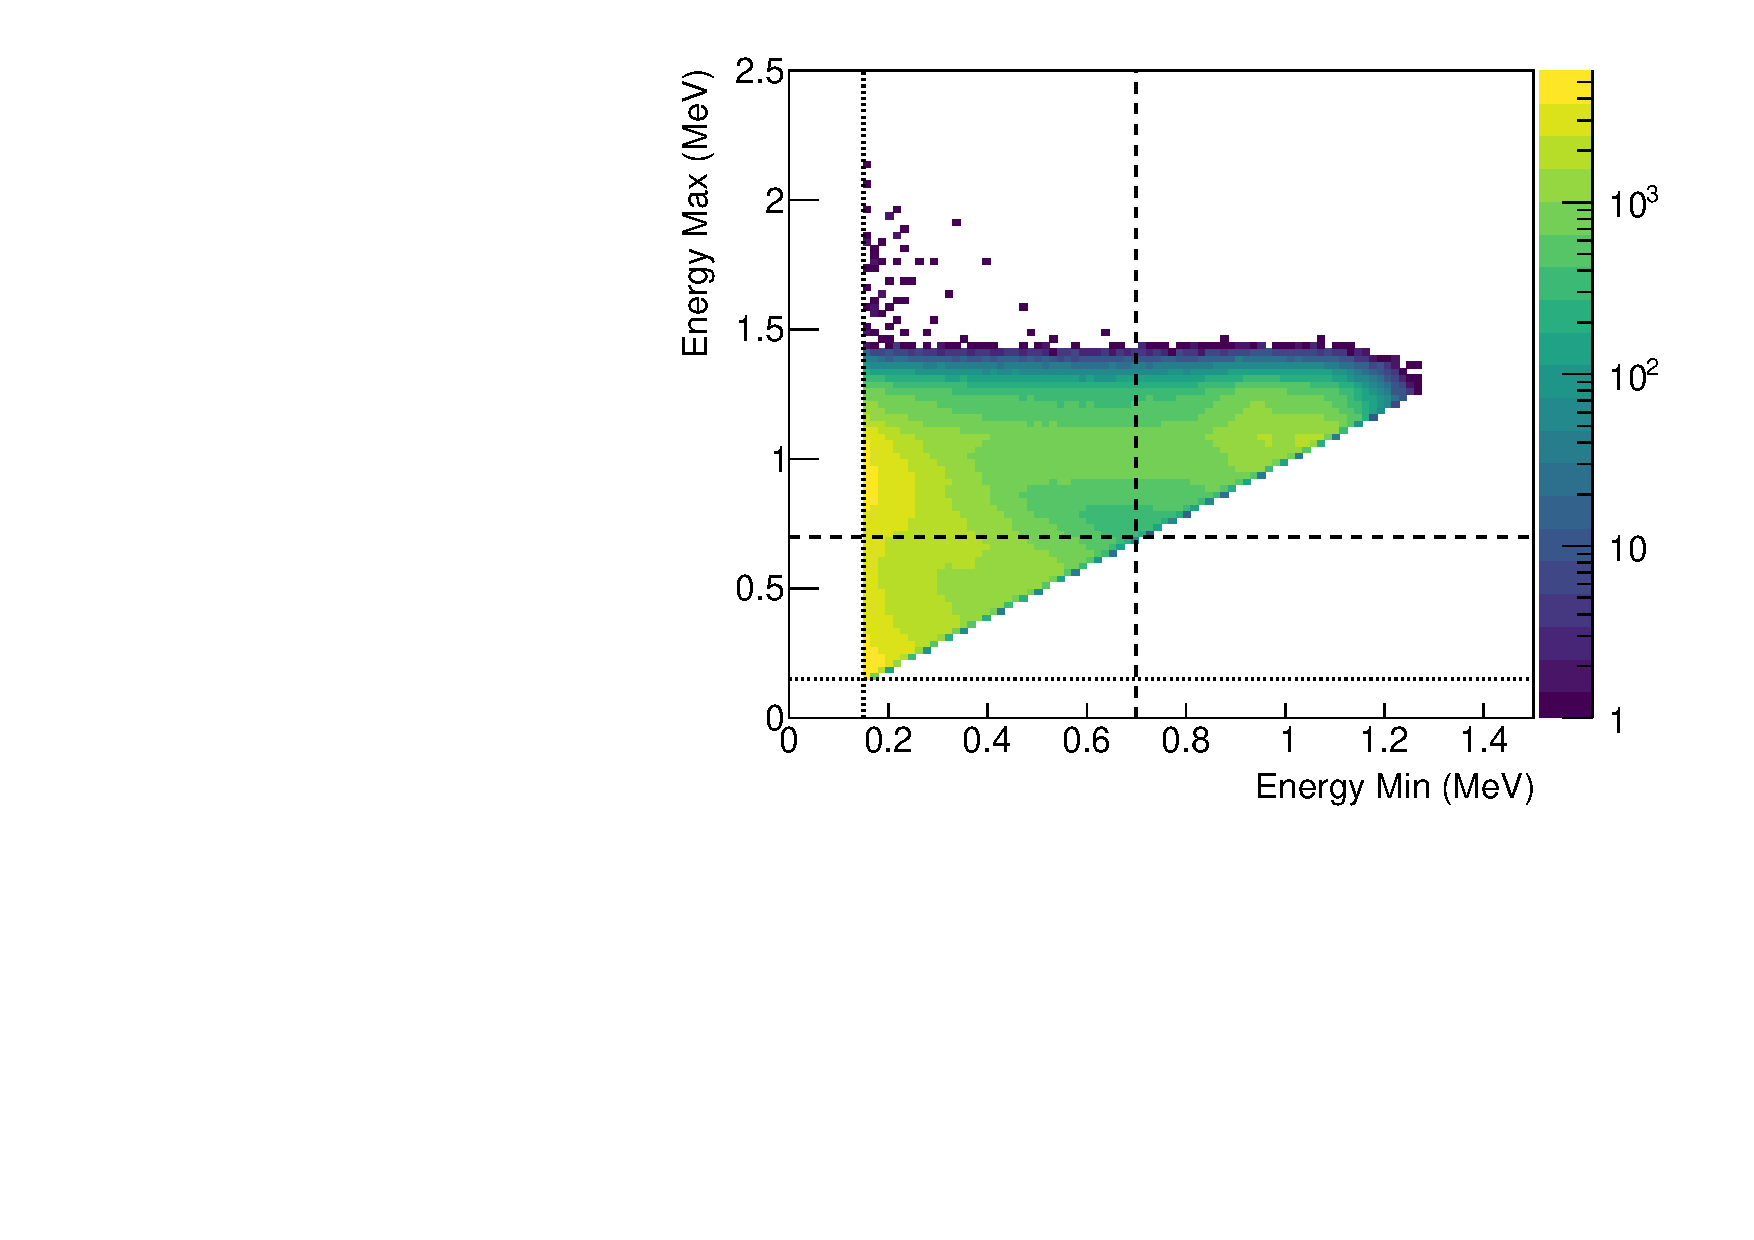
\includegraphics[width=14cm]{commissioning/fig_commissioning/Co_energy_cut.pdf}
    \caption{Maximal energy with minimal energy, for simulated Cobalt events, with source in position $5$ (see Fig.~\ref{subfig:Co_setup_wall}).
      High threshold is represented in black dotted line.
      Dashed lines materialise the individual energy selection.
      \label{fig:Co_energy_cut}}
  \end{figure}
  The high energy threshold is represented by two black dotted lines.
  The topology of interest is observable with two hits around $1$~MeV.
  Also, events where two successive Compton interactions of a single photon from Cobalt occur in two different optical modules are characterised by a high energy hit ($\sim 0.8$ MeV), and a low energy hit ($\sim 0.2$ MeV).
  This topology constitutes a background for this analysis.
  In order to reject them, given the energies of the two interesting Cobalt photons, we only select individual calorimeter hit energies greater than $0.7$ MeV.
  This individual energy selection is pictured by two black dashed lines.
  It naturally highly depends on the calorimeter energy calibration.
  %% If this energy selection is aims to reject \Co\ $\gamma$ particles, but not for background such as \Tl.
\item Geometrical selection:
  with a detector well calibrated in energy, the previous selection is sufficient to prevent double Compton interactions to be selected.
  But, at the time of the data-taking, the detector was not fully calibrated.
  The energy of some reconstructed particle hits then might be badly estimated and some background events could pass this energy selection.
  As such intercations occur predominantly in two close scintillators, we reject topologies where two neighbouring optical modules detect signal in the coincidence window.
  The detector energy calibration is discussed in Sec.~\ref{subsec:Co_energy_calib}.
\end{itemize}
These four selections are intended to improve the Cobalt signal to background ratio.
The coincidence time selection is only applied to real data, while others are applied both to simulations and real data.
Indeed, what we call an \emph{event} does not have the same meaning depending on whether we are talking about simulation or real data.
We simulate a given amount of disintegrations at given location(s) of the detector, so the definition of a Monte Carlo event is straightforward, and concepts such as the pile up has no sense.
For real data acquisitions, a set of criteria have to be established in order to define what an event is, as the time coincidence window for example.

We remind the signification of selection efficiency $\epsilon$ which is
\begin{equation}
  \epsilon = \frac{\text{Number of selected events}}{\text{Total number of events}}\,.
\end{equation}
Selection efficiencies are presented in table~\ref{tab:Co_cut_eff}.
\begin{table}[h]
  \centering
  \begin{tabular}{|c|c|c|c|}
    \hline
    & Simulations & Data \\
    \hline\hline
    High thresold & $35.7$\% & $98.0$\% \\
    Individual energy & $17.0$\% & $70.2$\% \\
    Geometrical & $16.5$\% & $61.0$\% \\
    \hline
  \end{tabular}
  \caption{Selection efficiencies for simulations and real data.
    \label{tab:Co_cut_eff}}
\end{table}
Significant differences are observed between simulations are real data, mainly due to the energy calibration.
Indeed, at the time of the data taking, the gain equalisation and energy calibration were preliminary and had to be improved.
Therefore, this statement directly affect the reconstructed energies of calorimeter hits.
We address this question in Sec.~\ref{subsec:Co_energy_calib}.

%% simus
%% before = 1000001 side = 917239 main = 907700 mult = 35061 event_deltat = 35061


\subsection{Background estimation}
\label{subsec:bkg_estimation}

The signal for this analysis is composed two $\gamma$'s of $1.17$ MeV and $1.33$ MeV, emitted after Cobalt disintegrations.
After application of the four selections, it is primordial to estimate and characterise the remaining background in the selected topology, detected by the calorimeter during the data acquisition.

\subsubsection*{Types of background}

Mainly three different types of background can be harmful for this analysis, all pictured in Fig.~\ref{fig:Co_bkg}.
\begin{figure}[h]
  \centering
  \begin{subfigure}[t]{0.30\textwidth}
    \centering
    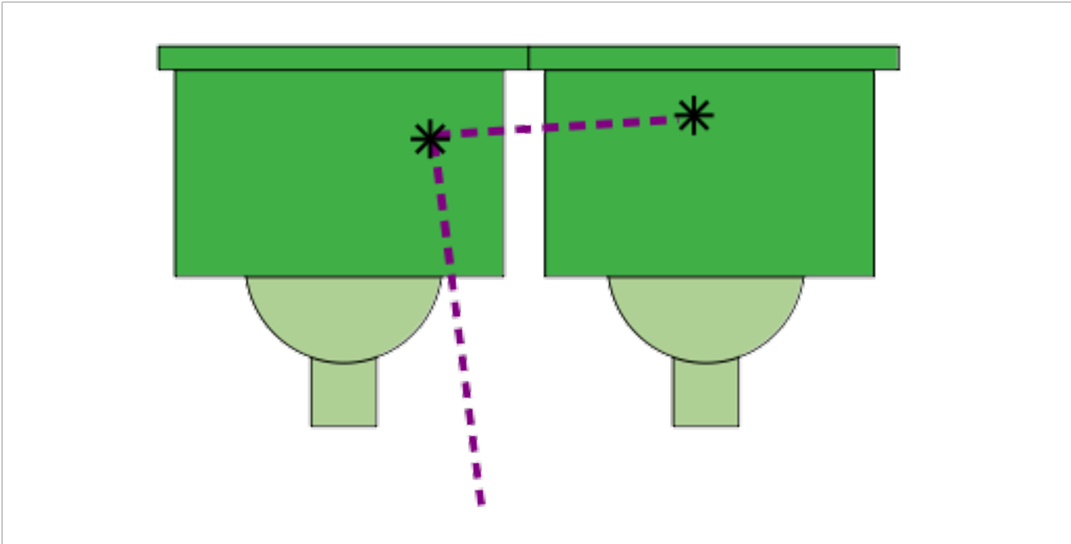
\includegraphics[height=0.50\textwidth]{commissioning/fig_commissioning/Co_bkg_1.pdf}
    \captionsetup{justification=justified}
    \caption{
      \label{subfig:Co_bkg_1}}
  \end{subfigure}
  \hfill
  \begin{subfigure}[t]{0.30\textwidth}
    \centering
    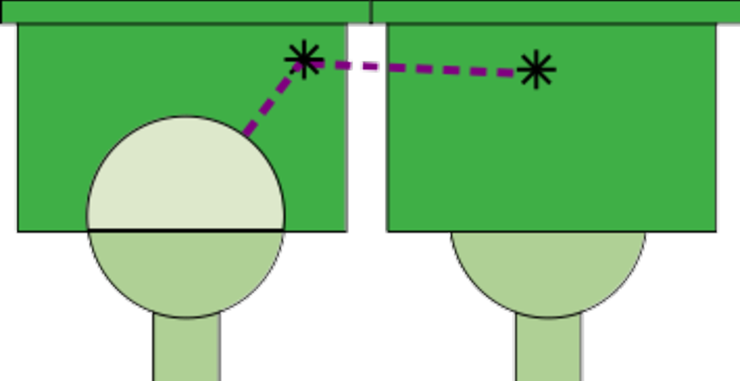
\includegraphics[height=0.50\textwidth]{commissioning/fig_commissioning/Co_bkg_2.pdf}
    \captionsetup{justification=justified}
    \caption{
      \label{subfig:Co_bkg_2}}
  \end{subfigure}
  \hfill
  \begin{subfigure}[t]{0.30\textwidth}
    \centering
    \includegraphics[height=0.50\textwidth]{commissioning/fig_commissioning/Co_bkg_3.pdf}
    \captionsetup{justification=justified}
    \caption{
      \label{subfig:Co_bkg_3}}
  \end{subfigure}
  \caption{Background types for the Cobalt study.
    Interactions of photons in scintillators are represented by black stars.
    (a) Interaction of a single Cobalt photon in two scintillators through double Compton scattering.
    (b) Interaction of a photon coming from natural radioactive isotopes contamination (PM glass...), through double Compton scattering.
    (c) Interactions of two uncorrelated photons, coming from the demonstrator outside (natural radioactivity of laboratory rock...), in two scintillator blocks
    \label{fig:Co_bkg}}
\end{figure}
\begin{itemize}
\item Through a double Compton interaction, a single Cobalt $\gamma$ particle can deposit energy in two scintillator blocks (see Fig.~\ref{subfig:Co_bkg_2}).
As described in Sec.~\ref{subsec:Co_datacut}, the geometrical and individual energy selections have been set up to reject these background events.
\item Photons coming from the natural radioactive decay chains of $^{238}$U, $^{232}$Th and $^{40}$K isotopes.
Typically, the $2.61$ MeV-$\gamma$, from \Tl\ decay, can interact successively in two scintillators through Compton scatterings and produce high energy events (see Fig.~\ref{subfig:Co_bkg_1}).
These disintegration can occur in the source foils or in the detector's components (mainly PM glass).
\item At the time of the data acquisition, the calorimeter was in commissioning phase, and the iron shielding was not yet installed.
Therefore, the calorimeter was not properly protected from external particles, coming from outside the detector (radioactive isotope contamination of laboratory rock).
Accidental events where two decorrelated $\gamma$ particles, can be detected in two scintillator blocks (see Fig.~\ref{subfig:Co_bkg_3}).
The coincidence time window should avoid these accidental to be selected.
\end{itemize}
All these three topologies can mimic the Cobalt two-$\gamma$'s signal.

Estimating the amount of background received by optical blocks during the acquisition is essential to assess our results.
In order to characterise the two last types of background (decorrelated from the Cobalt source), an acquisition without the Cobalt calibration source has been performed (see Sec.\ref{subsec:Co_setup}).
Unfortunately, be owing to optical modules gain issues, these data are not usable.
Therefore, we use the data acquisition taken with the Cobalt source set behind the wall to estimate this background.

\subsubsection*{Background characterisation}

When the Cobalt source is set behind the wall, collected data may contain signal events coming from it as well as background events.
Let us assume these background events are dominated by radiocative decays and external $\gamma$'s, by considering the background coming from double Compton intercations of Cobalt $\gamma$'s have been efficiently removed by application of the individual energy cut.
We choose to modelise the Cobalt data as a linear combination of signal events $s$ and background events $b$
\begin{equation}
  \hat{d}=s+b\,,
  \label{eq:estimation_data}
\end{equation}
where $s$ and $b$ are thus considered as uncorrelated.
The question is how to extract informations about background, using the Cobalt data acquisitions?
We remind the Cobalt source was placed at different positions behind the calorimeter wall (Fig.~\ref{subfig:Co_setup_wall}, Sec.~\ref{subsec:Co_setup}).
We aim to take advantage of those different configurations to reach our goal.
In the following, we make use of the positions $2$ and $8$ for the Cobalt source.
Therefore, depending on whether the source is in one of the two positions, some optical modules are \emph{close} to it, others are \emph{far}.
More precisely, we consider as \emph{close}, the optical modules that are separated from the source by less than 10 OMs (i.e. less than half the wall-lenght), the others being \emph{far} from it\footnote{For example, an optical module located on the left (right) of the calorimeter wall, is considered as far from (close to) the source, if the source is in position $8$.}.
Considering that, we distinguish two categories of data, $\hat{d}^{\,\text{close}}$ and $\hat{d}^{\,\text{far}}$, defined as the estimations of data events detected by an optical module when the source is close to, or far from it, respectively.
Then, we precise our data modelisation with
\begin{equation}
  \hat{d}^{\,\text{close}} = b + s^{\,\text{close}}\,,
  \label{eq:estimation_data_close}
\end{equation}
where $s^{\,\text{close}}$ is naturally the number of signal Cobalt events detected by a given optical module for which the distance from the source, $D_{\,\text{source}}$, is lower than $10$.
In the same way, considering $s^{\,\text{far}}$ as signal events detected by an optical module from which the source is far, we have
\begin{equation}
  \hat{d}^{\,\text{far}} = b + s^{\,\text{far}}\,.
  \label{eq:estimation_data_far}
\end{equation}
Estimations of $s^{\,\text{close}}$ and $s^{\,\text{far}}$ (respectively noted $\tilde{s}^{\,\text{close}}$ and $\tilde{s}^{\,\text{far}}$) are provided using simulations of \Co\ events in positions $2$ or $8$.
Indeed, as we consider the double Compton interaction background as negligible, the amount of signal events received for optical modules far or close from the source can be established with Cobalt simulations.
Then, the coefficient $\alpha$ defined as
\begin{equation}
  \alpha = \tilde{s}^{\,\text{far}}/\tilde{s}^{\,\text{close}}\,.
\end{equation}
It depends on the distance $D_{\,\text{source}}$ and is found to be $0.05 \% < \alpha < 5 \%$, meaning that the number of simulated signal events detected by optical modules distant from the source is greatly lower than for close optical modules, for a given source position.

In order to provide a non-biased estimation of $b$, given the data model in Eq.~\eqref{eq:estimation_data_far}, we would remove $\tilde{s}^{\,\text{far}}$ (estimated through simulations) from $\hat{d}^{\,\text{far}}$ (estimated with Cobalt data acquisition).
However, qualitatively comparing data and simulations is not straightforward, especially due to detector efficiency considerations, discussed in Sec.~\ref{subsec:detector_efficiency}.
%%on voudrait avoir b=dfar, mais c'est biaisé pcq il reste signal. On pourrait enlever sfar, mais
%%c'est la merde de faire ça avec les simus
Nevertheless, we can give an order of magnitude of the amount of background events detected.
To do so, we display in Fig.~\ref{fig:Co_data_bkg} the number of calorimeter hits, after data selection, counted by each optical module, as a function of the distance to the Cobalt source.
\begin{figure}[h]
  \centering
  \includegraphics[width=1.1\textwidth]{commissioning/fig_commissioning/Co_data_bkg.eps}
  \caption{Number of events for pairs of OMs on the source side and on the opposite source side, for real data (green) and simulated data (red), as a function the distance to the source (in units of number of OM).
    The vertical dotted line materialises the distance limit of $10$ OMs from the source.
    \label{fig:Co_data_bkg}}
\end{figure}
The $10$ OMs limit is materialised by a vertical dashed line.
Calorimeter hits that occurred in coincidence above and below this limit are displayed both for simulated and real data.
Therefore, events where the two hits occur in two optical modules, each located in one half of the calorimeter, are not represented.
This explains the observable gap at the $10$ OMs limit level.

We first focus on simulation results.
Calorimeter hits for which $D_{\,\text{source}}<10$, represent the estimation of the amount of signal events detected close to the source, $\tilde{s}^{\,\text{close}}$.
Similarly, hits for which $D_{\,\text{source}}>10$ embed for $\tilde{s}^{\,\text{far}}$, the amount of signal events remaining for optical modules far from the calibration source site.
As expected, the number of signal Cobalt events decreases with the distance to the source.

We then compare data events with simulations.
Calorimeter hits for which $D_{\,\text{source}}<10$ materialise the number of data events estimation $\hat{d}^{\,\text{close}}$.
Apart from slight differences, discussed in Sec.~\ref{subsec:detector_efficiency}, these data events follow the same evolution as signal events with the distance to the source.
This leads us to conclude that optical modules close to the source are dominated by Cobalt signal events.
Similarly, $D_{\,\text{source}}>10$ events stand for $\hat{d}^{\,\text{far}}$.
We observe that $\tilde{s}^{\,\text{far}}/\hat{d}^{\,\text{far}} \ll 1$, which is compatible with the $\alpha$ coefficient values, being $5\%$ in the worse case, explaining the few amount of $\tilde{s}^{\,\text{far}}$ events remaining for optical modules far from the source.
Moreover, we find that the amount of $\hat{d}^{\,\text{far}}$ events is globally stable with the distance to the source.
Therefore, we assume that optical modules away from the \Co\ source by more than $10$ OMs are background dominated.
As this amount of background is comparable for all optical modules, regardless of their distance to the source, we conclude that these events are decorrelated from the Cobalt source, and come from other sources (as external $\gamma$'s).
%% donc bkg qui ne vient pas de la source
Therefore, for a $25$ minutes run, each optical module detects around $10^{2}$ external background events.
%% différence data/simus dans close : gain equalization ptetre pas dégueu sinon on verrait une diff
%% à ce niveau là. gain equalisation of optical modules, discussed in Sec.~\ref{sec:comm_energy_calibration}, could impact greatly the .

To sum up these results, calorimeter hits for optical modules close to the Cobalt calibration source are, for the most part, signal events.
Besides, hits occurring far from the source are predominantly background events.
As we moved the source in different positions, we have access to the estimation of background rate $\hat{b}$ for each optical module (when the source is far), and to the estimation of $\hat{s}$ (when the source is close).
Therefore, we can compute the signal to background ratio, as a function of the distance to the Cobalt source, displayed in Fig.~\ref{fig:Co_ratioSB}.
\begin{figure}[h]
  \centering
  \includegraphics[width=1.1\textwidth]{commissioning/fig_commissioning/Co_ratioSB_distance.pdf}
  \caption{Signal to background ratio for each optical module, as a function of the distance to the Cobalt source.
    \label{fig:Co_ratioSB}}
\end{figure}
The number of signal events in each optical module depends on the distance to the source, which is not the case for the number of background events, explaining the decreasing of $S/B$ with $D_{\,\text{source}}$.
%% on mesure alpha et il est petit donc on peut négliger sfar dans la modélisation

To summarise, in this subsection, we gave informations on background events for the whole French wall, using data taken with the Cobalt source set at different positions.
We confirmed our assumption that the more one optical block is far from the source, the less it detects $\gamma$ particles emitted after Cobalt disintegrations, then the more the signal to background ratio decreases.
In the following, in order to properly compare simulated and real data, we give an order of magnitude of the detector efficiency during the data-taking with the Cobalt source.

%% faut dire que du coup on peut croire nos résultats quand la source est proche pour l'analyse time reso
%% aussi : Remarque : dans la suite (mesure des sigma_t), tu pourrais faire l'analyse pour les blocs
%% qui vérifient S/B > 10

%% dire qu'on peut faire ça avec d'autres runs mais que c'était pour avoir un ordre d'idée

%%Remarque : le bruit de fond peut décroitre sur les bords - ex : 2-3 dernières colonnes de PM (et
%%c'est un peu ce que tu vois sur la figure 7.8)

%% *Dire que ç'aurait été mieux de prendre un OM de ref pcq là on moyenne mais pas poss car pas de stat*
%% * finir: l'idée c'est de dire sortir un spectre en énergie data+estimation du bdf avec ce qu'on vient de faire.
%% Je vais prendre toutes les paires d'OMs possibles pour les OMs loin de la source, et tracer leur spectre en énergie en coincidence.
%% ça va me donner un histogramme binné sur l'énergie, et chaque bin aura une certaine dispersion, qui vient des différences des spectres en énergie des OMs\\



\subsection{Detector efficiency}
\label{subsec:detector_efficiency}

%% parler de la baisse d'eff du à la saturation de l'acqu
%% *A mettre quelque part:
%% the energy calibration discussed in Sec.~\ref{sec:comm_energy_calibration} was not completed, and optical modules' gains were not all aligned.*

The last step before going into detail in optical modules' timing resolution study is to determine the detector efficiency of the SuperNEMO demonstrator, during the Cobalt acquisition week.

Standing as an example, we compare real and simulated energy spectra for a given pair of optical modules detecting events in coincidence.
We provide these spectra in Fig.~\ref{fig:detector_efficiency}, where events satisfy to the four criteria described in Sec.~\ref{subsec:Co_datacut}, for the Cobalt source in position $5$.
\begin{figure}[h]
  \centering
  \includegraphics[width=17cm]{commissioning/fig_commissioning/Co_efficiency_detector.pdf}
  \caption{Top pad: energy spectra for simulated data (orange solid line) and real data (purple solid line) in logarithmic scale.
    Bottom pad: ratio of real data over simulated data for each bin in logarithmic scale.
    \label{fig:detector_efficiency}}
\end{figure}
The simulated data are normalised to the source activity and acquisition time.


Firstly, the energy resolution of the calorimeter blocks.
Secondly, at the time of the data taking, optical modules where not equalised in gain.
The real data energy spectrum is also characterised by a high energy part.
This may be due to external background events, which are not taken into account in the simulated data.
In Sec.~\ref{subsec:bkg_estimation} is presented a background analysis to investigate the high energy part of the energy spectrum, and better understand the data.


%% Given the amount of real and simulated events, we conclude that the detection efficiency is $29$\%.
%% Numerous parameters can affect the detection efficiency.
%% \begin{itemize}
%% \item Read out efficiency is mainly driven by
%% \end{itemize}



%% Efficiency is going to be improved.


* a finir *

\subsection{Energy calibration}
\label{subsec:Co_energy_calib}



\subsection{Determination of the individual timing resolution of each optical module}

%% Optical modules have been characterised before installation.
%% Performing simulations of \Co\ disintegration

\subsubsection*{Time difference distributions}

The final goal of this analysis is to determine the time resolution of optical modules, due to the scintillator time dispersion.
As displayed in Fig.~\ref{fig:Co_decay_scheme}, the two photons of Cobalt $60$ are emitted in coincidence.
The selections described in Sec.~\ref{subsec:detector_efficiency} aim to maximise the signal to background ratio, the signal being the detection of two $\gamma$'s interacting in two different optical modules.
The two $\gamma$'s, travelling at speed of light in air, reach the two optical modules at two different times.
The time of a calorimeter hit $t^{\gamma}_{i}$, describes in Fig.~\ref{fig:CFD} in Chapter~\ref{ch:commissioning}, is defined from the collected charge sampling at PM anode and received by the electronic readout.
%% We are interested in event topologies where the two $\gamma$'s of Cobalt $60$ hit two different calorimeter blocks.
We then look for topologies where two calorimeter hits occurred in a given time window of $62.5$ ns.
This coincidence time window where chosen to select the two Cobalt $\gamma$'s coincidence events, avoiding accidentals.
A first event occur in one of the scintillator of the wall, meaning the amount of charge is high enough to pass the high amplitude threshold.
In the considered coincidence time window, a second particle interacts in another scintillator.
This topologies are likely to happen for all combinations of pairs of PMs (given the distance between the two optical modules).
Therefore, we can construct a $\Delta t^{\text{pair}}$ distribution for each pair of OM, defined as the time difference between two calorimeter hits $\Delta t^{\text{pair}} = t^{\gamma}_{A} - t^{\gamma}_{B}$.
Here, one of the two optical modules, namely the $A$, is chosen as reference.

In Fig.~\ref{fig:Co_deltat} is presented an example of a $\Delta t^{\text{pair}}$ distribution, for a given pair of optical modules, both for the simulated and real data, with the Cobalt source placed at the central position behind the calorimeter wall.
%% on ne regarde des coincidences que pour paires OM sur un même mur
\begin{figure}[h]
  \centering
  \includegraphics[width=15cm]{commissioning/fig_commissioning/Co_deltat_distrib_ex.eps}
  \caption{$\Delta t^{\text{pair}}$ distributions for real data (green solid line) and simulated data (dark red solid line).
    Two Gaussian fits (orange and blue dotted line) are displayed and fit parameters are given in the legend.
    The two distributions do not have the same mean because optical modules are not aligned in time.
    However, this does not disturb the time resolution measurements.
    \label{fig:Co_deltat}}
\end{figure}
The two distributions present different behaviours in terms of means and standard deviations.
This can be explained by two distinct reasons.

Firstly, as exposed in Sec.~\ref{subsec:OMtimeResponse}, in the framework of this study, the calorimeter part of the SuperNEMO demonstrator was considered as perfect in terms of time reconstruction, in the simulation processed.
All optical modules' time resolutions, whose main contributions are presented in Sec.~\ref{subsec:OMtimeResponse}, were set to $0$ ns.
We retrieve such a setting in the $\Delta t^{\text{pair}}$ distribution for simulated data.
As a consequence, the standard deviation, for this pair of optical module, is higher for real data than for simulated data.
Even though the case presented is just an example for a given pair of OM, we will see this is a general result for all pairs of optical modules.

Secondly, at this time, some differences remain between what is simulated and the real demonstrator performances.
In fact, as the demonstrator is in commissioning phase, some calorimeter detection characteristics are not yet included in the Falaise simulations, and affect the real data results (characterisation of optical modules' energy resolution, implementation of particle time-of-flight shifting due to coaxial cables...).
We observe such differences in the two distributions means: the data distribution is shifted by $3.7$ ns compared to the simulation distribution.
This result was expected: for the moment, the Falaise software does not take into account, in the reconstruction process, the time made by the electric signal to travel from a PM divider to the electronic readout, discussed in Sec.~\ref{sec:reflecto} of Chapter \ref{ch:commissioning}.
In other words, the time difference distribution for a given pair of optical module is affected by the difference of lengths of the two coaxial cables.
This is an important parameter directly affecting the mean time difference between two distinct optical modules detecting particles in coincidence.
Although simulations do not perfectly picture the full detector performances, real data and simulation can be compared, since we understand these differences.
Moreover, both the real and simulated data are affected by parameters such as the distance from the Cobalt source to the wall, or the distance between the two considered optical modules.

A $\Delta t^{\text{pair}}$ distribution exists for each pair of optical modules detecting two events in the time coincidence window.
The least square method is used to fit the distributions, which minimises the difference between the measured value and the fitted value.
A mean and a standard deviation is then defined for each pair of optical module whose fitted data has $\chi^{2}/\text{dof}<4$.
Therefore, each pair of optical module is characterised by the mean and standard deviation of its corresponding $\Delta t^{\text{pair}}$ distribution.
The standard deviation, noted as $\sigma_{t}^{\text{pair}}$ in the figure legend, corresponds to the uncertainty on time measurement for this peculiar pair of OM.
Therefore, a value of the time uncertainty $\sigma_{t}^{\text{pair}}$ can only be given for a proportion of total optical modules.

As the detector in commissioning phase, the acquisition was taken with $254$ optical modules\footnote{Three OMs are damaged on the French wall (*ref commissioning*) and three photomultipliers were not well aligned in gain at this time, and had to be removed from the analysis.}.
In this study, we only consider $8$ inches PMs, hence this analysis aims to characterise the time resolution of $214$ OMs, representing $22791$ different possible combinations of pairs.
In Fig.\ref{fig:Co_corr_sigma} are presented the $\sigma_{t}^{\text{pair}}$ values, both for simulated and real data.
\begin{figure}[h]
  \centering
  \includegraphics[width=15cm]{commissioning/fig_commissioning/Co_corr_sigma.eps}
  \caption{$\sigma_{t}^{\text{pair}}$ distribution for pairs of optical modules.
    \label{fig:Co_corr_sigma}}
\end{figure}
In the first place, we notice the mean $\sigma_{t}^{\text{pair}}$ value for simulations is lower than for real data.
As explained above, this difference is caused by the perfect calorimeter time resolution for simulations on one side, and by the detector characteristics not yet implemented in the simulation software on the other side.
This second statement is also behind the larger value of the real data distribution's standard deviation.
In fact, for the simulated case, $\Delta{t}$ distributions, of which an example is given in Fig.~\ref{fig:Co_deltat}, have comparable $\sigma_{t}^{\text{pair}}$ values, for all pairs of optical modules.
This is not the case for the real data: the $\sigma_{t}^{\text{pair}}$ value for a given pair of OM depends on the difference between the two coaxial cable lengths.
And this length difference being specific for each pair of optical module.

Moreover, we succeeded characterising $\sigma_{t}^{\text{pair}}$ values for $26$\% of pairs of optical blocks for real data, against $87$\% for simulations.
In fact, the more one optical module is from the source, the more it is background dominated.
As we explained, such a value is provided for a OM pair only if the fit of the corresponding $\Delta t^{\text{pair}}$ distribution is of high-quality.
Therefore, the optical modules for which the fit successes are the ones around the source.
This is not valid for simulations are we only have Cobalt events, and no background is simulated.

In Fig.\ref{fig:Co_sigma_distance} is displayed the number of characterised optical blocks, with the distance between the reference block and the Cobalt $60$ source, in units of block width.
\begin{figure}[h]
  \centering
  \includegraphics[width=15cm]{commissioning/fig_commissioning/Co_sigma_distance.eps}
  \caption{Number of characterised OM pairs, as a function of the distance between reference OM and source.
    \label{fig:Co_sigma_distance}}
\end{figure}
For a given distance from the source, the amount of characterised OM is lower for the real data case than for the simulated one.
This explains the different amount of characterised OMs for real and simulated data.

We presented results on the uncertainty on time measurement for pairs of optical module, $\sigma_{t}^{\text{pair}}$.
However, we are interesting in providing such values, independently for each optical modules.
Therefore, in the following, we present the algorithm we used to provide $\sigma_{t}^{\text{indep}}$ values.



%%fig distrib mean and sigma

\subsubsection*{Decoupling of $\sigma_{t}^{\text{pair}}$ values}

We have determined $\sigma_{t}^{\text{pair}}$ for some of the pairs of OMs on the French wall.
For example, if we take the source closest OM (OM located at the centre of the French main calorimeter wall), it has coincidence events with a certain number of other optical blocks.
Among them, $119$ different $\Delta t^{\text{pair}}$ distributions are fitted, therefore $119$ values of $\sigma_{t}^{\text{pair}}$ are stored.
And this work is done for each counting optical module taken as reference.
All following steps aim to determine the individual $\sigma_{t}^{\text{indep}}$.

We want to evaluate this value for the closest OM from the source, let us number it $0$.
We have access to the number of coincidence events this OM has with each other OMs.
We pick up the two OM that have the larger number of coincidence events with this reference OM, with their associated $\sigma_{t}^{\text{indep}}$ and mean energies.
We number them as $1$ and $2$.
Therefore, to find the value of $\sigma_{t}^{\text{indep}}$, we have to solve a set of $3$ linear equations:
\begin{align}
  (\sigma_{t}^{0,1})^{2} &= \frac{(\sigma_{t}^{0})^{2}}{\bar{E_{0}}} + \frac{(\sigma_{t}^{1})^{2}}{\bar{E_{1}}}\nonumber \\
  (\sigma_{t}^{0,2})^{2} &= \frac{(\sigma_{t}^{0})^{2}}{\bar{E_{0}}} + \frac{(\sigma_{t}^{2})^{2}}{\bar{E_{2}}}\\
  (\sigma_{t}^{1,2})^{2} &= \frac{(\sigma_{t}^{1})^{2}}{\bar{E_{1}}} + \frac{(\sigma_{t}^{2})^{2}}{\bar{E_{2}}} \nonumber\,,
  \label{eq:Co_sigma}
\end{align}
where $\sigma_{t}^{i}$ is the individual uncertainty on time measurement for the block $i$.
Solving simultaneously these equations comes down to diagonalise the matrix $S$ defined as
\begin{equation}
  S =
  \begin{pmatrix}
    1/\bar{E_{0}} & 1/\bar{E_{1}} & 0 \\
    1/\bar{E_{0}} & 0 & 1/\bar{E_{2}} \\
    0 & 1/\bar{E_{1}} & 1/\bar{E_{2}}
  \end{pmatrix}
  .
\end{equation}

We now generalise this method to all possible combinations of OM pairs for which we have informations on $\sigma_{t}^{\text{pair}}$.

\subsubsection*{Estimating the variance}



\subsection{Conclusion}
\begin{itemize}
\item il fauddrait au moins tenir compte du bdf qui est les decays de la source
\item il nous faut des simus bkg
\item il nous faut un run bkg
\item ça marche bien
\item il faudrait refaire une manip avec PMs alignés
  \item On aurait pu décorréler les sigmas en utilisant toutes les combinaisons possibles, mais il aurait fallu faire masse de simus pour déterminer les covariances
\end{itemize}


%%%%%%%%%%%%%%%%%%%%%%%%%%%%%%%%%%%%%%%%%%%%%%%%%%%%%%%%%%%%%%%%%%%%%%%%%%%%%%%%%%%%%%%%%%%%%%%%%%%%%%%%%%%%%%%%%%%%%%%%%%%%%%%%
\section{The Light Injection System}
\label{sec:LIS}



\subsection{Light injection system commissioning}


In the LI system design, the SuperNEMO demonstrator has been segmented in $10$ areas.
Each area receives light from one given LED

Primary/secondary
Each LED lights
Group LEDs/area



\subsection{Time resolution of optical modules}



%% \begin{figure}[h]
%%   \centering
%%   \includegraphics[width=10cm]{commissioning/fig_commissioning/}
%%   \caption{
%% \label{fig:}}
%% \end{figure}



%% \begin{figure}[h]
%% \centering
%% \begin{subfigure}[t]{0.48\textwidth}
%%   \centering
%%   \includegraphics[width=1.1\textwidth]{commissioning/fig_commissioning/}
%%   \captionsetup{justification=centering}
%%   \caption{
%%     \label{subfig:}}
%% \end{subfigure}
%% \hfill
%% \begin{subfigure}[t]{0.48\textwidth}
%%   \centering
%%   \includegraphics[width=1.1\textwidth]{commissioning/fig_commissioning/}
%%   \captionsetup{justification=centering}
%%   \caption{
%%     \label{subfig:}}
%% \end{subfigure}
%% \caption{
%%   \label{fig:}}
%% \end{figure}


               \begingroup
               \setlength{\beforechapskip}{-35pt} % or any other dimension
               \chapter*{Conclusion}
\addcontentsline{toc}{chapter}{Conclusion}

               \endgroup

               \chapter*{Résumé}
\addcontentsline{toc}{chapter}{Résumé}


               \bibliographystyle{unsrt}
               \bibliography{bibliography_thesis}

               \end{document}
